\documentclass[11pt,aspectratio=169]{beamer}

% --- Tema og fonte ---
\usetheme{Madrid}
\usefonttheme{serif}
% --- Farver ---
\definecolor{myteal}{RGB}{14,71,57}
\setbeamercolor{title}{fg=white}
\setbeamercolor{frametitle}{fg=white,bg=myteal}
\setbeamercolor{block title}{fg=white,bg=myteal}
\setbeamercolor{block body}{bg=myteal!10}
\setbeamercolor{normal text}{fg=myteal}
\setbeamercolor{background canvas}{bg=white}
\setbeamercolor{structure}{fg=myteal}
\setbeamercolor{palette primary}{fg=white,bg=myteal}
\setbeamercolor{palette secondary}{fg=white,bg=myteal!80}
\setbeamercolor{palette tertiary}{fg=white,bg=myteal!60}
\setbeamercolor{author in head/foot}{fg=white,bg=myteal}
\setbeamercolor{title in head/foot}{fg=white,bg=myteal!80}
\setbeamercolor{date in head/foot}{fg=white,bg=myteal!60}
\setbeamercolor{titlelike}{fg=myteal}
\setbeamercolor{section in toc}{fg=myteal}
\setbeamercolor{item}{fg=myteal}
% --- Sprog og encoding ---
\usepackage[utf8]{inputenc}
\usepackage[danish]{babel}
\usepackage[T1]{fontenc}
\usepackage{lmodern}
% --- Matematik ---
\usepackage{amsmath,amsfonts,amssymb}
% --- Grafik og layout ---
\usepackage{graphicx}
\usepackage{ragged2e}
\usepackage{booktabs}
\usepackage{arydshln}
\usepackage[most]{tcolorbox}
% --- Ikoner og figurer ---
\usepackage{fontawesome5}
\usepackage{tikz}
\usetikzlibrary{positioning,arrows.meta,shapes.geometric,calc}
\usepackage{circuitikz}
% --- Positionering ---
\usepackage[absolute,overlay]{textpos}
% --- CSV ---
\usepackage{csvsimple}
% --- Kildehenvisning nederst på slides ---
\setbeamercolor{framesource}{fg=gray,bg=white}
\setbeamerfont{framesource}{size=\scriptsize}
\newcommand{\framesource}[1]{%
  \begin{textblock*}{12cm}(0.5cm,8.6cm)
    \raggedleft
    \beamercolorbox[wd=\textwidth,rightskip=0.5cm]{framesource}{#1}
  \end{textblock*}
}
% --- Automatisk billedattribution ---
\csvreader[
  head to column names,
  no head
]{Billeder/billedkilder.csv}{}{}
\newcommand{\billedkilde}[1]{%
  \csvreader[
    head to column names,
    full filter=\ifcsvstrcmp{\filnavn}{#1}{\csvfilteraccept}{\csvfilterreject},
    no head
  ]{Billeder/billedkilder.csv}{}%
  {%
    \tiny\forfatter\ / Wikimedia Commons (\licens)%
  }%
}
% --- Boksstile til jagttid-sliden ---
\tcbset{
  gruppe/.style={
    enhanced,
    colback=white,
    colframe=myteal,
    coltitle=myteal,
    boxrule=0.8pt,
    dashed,
    sharp corners,
    fonttitle=\bfseries\large,
    attach boxed title to top left={yshift=-2mm,xshift=3mm},
    boxed title style={colback=white,colframe=white,boxrule=0pt,sharp corners},
    top=1mm,left=1mm,right=1mm,bottom=1mm
  },
  felt/.style={
    enhanced,
    colback=white,
    colframe=myteal,
    boxrule=0.6pt,
    sharp corners,
    halign=center,
    valign=center,
    width=\linewidth,
    height=1.55cm,
    fit,
    fit algorithm=fontsize,
    fit basedim=7pt,
    boxsep=0.3mm,
    left=0.5mm, right=0.5mm, top=0.3mm, bottom=0.3mm
  },
  feltfri/.style={
    enhanced,
    colback=white,
    colframe=myteal,
    boxrule=0.6pt,
    sharp corners,
    halign=center,
    valign=center,
    width=\linewidth,
    boxsep=0.3mm,
    left=0.5mm, right=0.5mm, top=0.3mm, bottom=0.3mm,
    fontupper=\scriptsize
  }
}
% --- Matematiske operatorer ---
\DeclareMathOperator{\sen}{sen}
\DeclareMathOperator{\tg}{tg}
% --- Beamer-indstillinger ---
\setbeamertemplate{caption}[numbered]
\setbeamertemplate{navigation symbols}{}
% --- Forfatter ---
\author[Østerbro Jagttegn]{Østerbro Jagttegn \\ \textbf{Aleksander Sønder}}
% --- Hyperref (altid sidst) ---
\usepackage{hyperref}
\hypersetup{
  colorlinks=true,
  linkcolor=myteal,
  urlcolor=myteal,
  citecolor=myteal
}

\title{Obligatorisk Teori 3 \\
Hold: ss26}
\date{\today}

\begin{document}

% Titelside
\begin{frame}
  \titlepage
\end{frame}

% Indholdsfortegnelse (valgfri)
\begin{frame}{Program}
  \tableofcontents
\end{frame}

\section{Jagttermer - Del 1}

\begin{frame}
  \vspace{3em}
  \begin{center}
    {\LARGE \textbf{Jagttermer - Del 1}
    }
    \\
    \vspace{1em}
  \end{center}
\end{frame}


\begin{frame}{Jagttermer - Del 1 (A-F)}

\vspace{0.3em} % Mindre top-afstand

\begin{columns}[T]
    % --- Venstre kolonne: A-C ---
    \column{0.48\textwidth}
    \textbf{\large A, B, C}
    \setlength{\parskip}{0.1em} % Mindre afstand mellem punkter
    \scriptsize % Mindre skriftstørrelse
    \RaggedRight
    \begin{itemize}
        \item \textbf{Anskudssted:} Stedet, hvor vildtet blev ramt.
        \item \textbf{Anskyde:} Ramme vildt uden at skuddet er dræbende.
        \item \textbf{Afskydning:} Mængden af vildt skudt på et terræn.
        \item \textbf{Apport:} Kommando til hund om at hente nedlagt vildt.
        \item \textbf{Anstandsjagt:} Ventejagt fra et udvalgt sted.
        \item \textbf{Bagskud:} Skud til vildt, der løber/flyver direkte væk.
        \item \textbf{Bladet:} Primært træfområde på hårvildt (hjerte/lunger).
        \item \textbf{Brunsttid:} Tidsrummet, hvor parring foregår.
        \item \textbf{Brække op:} Åbne klovbærende vildt og tage indvoldene ud.
    \end{itemize}

    % --- Højre kolonne: D-F ---
    \column{0.48\textwidth}
    \textbf{\large D, E, F}
    \setlength{\parskip}{0.1em} % Mindre afstand mellem punkter
    \scriptsize % Mindre skriftstørrelse
    \RaggedRight
    \begin{itemize}
        \item \textbf{Doublé:} Nedlægge to stykker vildt i to skud i træk.
        \item \textbf{Esser:} Fødesøgning for hjortevildt og hare.
        \item \textbf{Fald:} 1) Ekskrementer 2) Stor ankomst af trækfugle.
        \item \textbf{Fangstskud:} Skud, der aflives anskudt vildt med.
        \item \textbf{Forende:} Dø (om vildt).
        \item \textbf{Forlægge:} Partere vildt (især klovbærende).
        \item \textbf{Fouragere:} Vildtets fødesøgning (andet end hjortevildt/hare).
        \item \textbf{Fællesjagt:} Organiseret jagt med et større antal deltagere.
    \end{itemize}
\end{columns}

\end{frame}

\section{Jagt fra kunstige skjul}

\begin{frame}
  \vspace{3em}
  \begin{center}
    {\LARGE \textbf{Jagt fra kunstige skjul}
    }
    \\
    \vspace{1em}
    Bekendtgørelse om udsætning af vildt, jagtmåder og jagtredskaber
    \\
    \vspace{1em}
    BEK nr 1652 af 19/12/2017, Kapitel 1
  \end{center}
\end{frame}

\begin{frame}
    \frametitle{Forbud mod jagt på pattedyr fra kunstige skjul (§ 1)}

    \vspace{1.5cm}

    § 1

    \vspace{0.5cm}

    Der må ikke drives jagt på pattedyr fra

    \vspace{0.5cm}

    1) kunstigt skjul, herunder hus, hytte, jordhul, eller

    \vspace{0.5cm}

    2) platform eller sæde, der er hævet mere end 50 cm over det omgivende terræn.

    \vspace{0.5cm}

    Med to undtagelser

    \vspace{2.5cm}
\end{frame}

\begin{frame}
    \frametitle{Varianter af kunstige skjul}

    \begin{columns}
        \column{0.5\textwidth}
        \centering
        \begin{figure}
            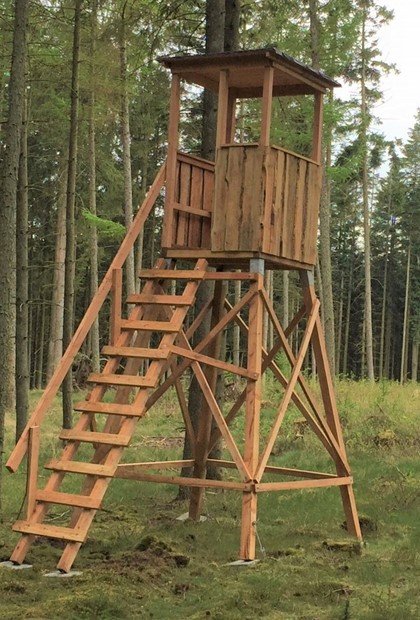
\includegraphics[width=0.5\textwidth]{Billeder/Redskaber/jagttårn.jpg}
            \caption{\textbf{Jagttårn} (jægeren kan skyde stående)}
        \end{figure}
        
        \column{0.5\textwidth}
        \centering
        \begin{figure}
            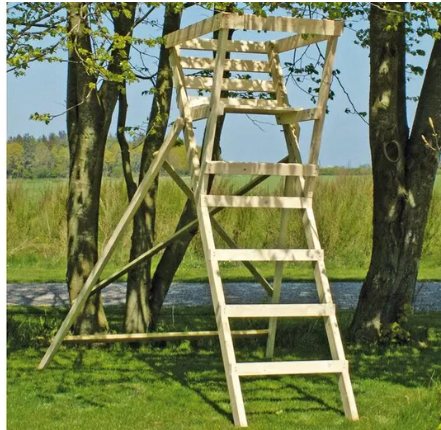
\includegraphics[width=0.5\textwidth]{Billeder/Redskaber/jagtstige.png}
            \caption{\textbf{Jagtstige} (jægeren kan skyde siddende)}
        \end{figure}
    \end{columns}

    \vspace{1cm}  % Plads til tekst under

    \centering
\end{frame}

\begin{frame}
    \frametitle{Regler for skydetårne (§ 1)}

    \begin{columns}[T]  % T for top-alignment
        \column{0.6\textwidth}
        \begin{itemize}
            \item Højere end 50 cm over omkringliggende areal
            \item Min 130 m til skel med mindre andet er aftalt skriftligt
            \item Udført i træ eller metal
            \item Opsættes i min 0,5 hektar skov eller ydre/inde skovbryn
            \item Må ikke skæmme (samme højde som øvrig bevoksning)
            \item Højde til plateau max 5m
            \item Sider max 110cm høje
            \item Plateau max 2 $m^2$
            \item Tag i et plan, ikke-reflekterende, max 10 cm udhæng
        \end{itemize}
        
        \column{0.4\textwidth}
        \centering
        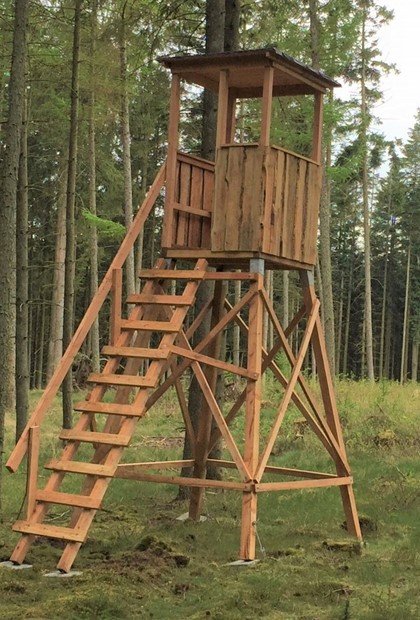
\includegraphics[width=0.7\textwidth]{Billeder/Redskaber/jagttårn.jpg}  % Mindre billede nu
        \vspace{0.5cm}
        \small 
    \end{columns}

\end{frame}

\begin{frame}
    \frametitle{Regler for skydestiger (§ 1)}

    \begin{columns}[T]  % T for top-alignment
        \column{0.6\textwidth}
        \begin{itemize}
            \item Højere end 50 cm over omkringliggende areal
            \item Min 130 m til skel med mindre andet er aftalt skriftligt
            \item De skal være mobile eller midlertidige konstruktioner
            \item Opsættes i hegn eller bevoksninger (ikke 0,5 hektar regel)
            \item Må ikke skæmme (samme højde som øvrig bevoksning)
            \item Højde til plateau max 5 m
        \end{itemize}
        
        \column{0.4\textwidth}
        \centering
        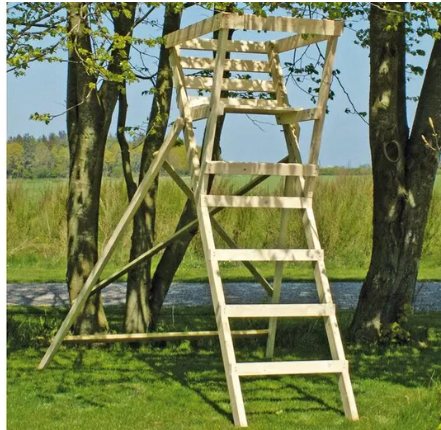
\includegraphics[width=0.7\textwidth]{Billeder/Redskaber/jagtstige.png}  % Mindre billede nu
        \vspace{0.5cm}
        \small 
    \end{columns}

    \end{frame}

\begin{frame}
    \frametitle{Regler for kunstige skjul på fugle (§ 3)}

    \begin{columns}[T]  % T for top-alignment
        \column{0.6\textwidth}
        \begin{itemize}
            \item Gulvet/ståstedet må højest være hævet 50 cm over terrænnet
            \item Ellers er kreativiteten ubegrænset – brug camouflage, net, siv, grene osv.
            \item Skjulet kan være midlertidigt (flytbart) eller mere fast (f.eks. ramme med net)
            \item Ofte brugt til andejagt, duejagt eller kragejagt med lokkefugle
            \item Husk at våbentype skal passe til skjulet (typisk haglgevær til fugle) (§ 2)
            \item Skjulet skal camouflages godt for ikke at skræmme vildtet
        \end{itemize}
        
        \column{0.4\textwidth}
        \centering
        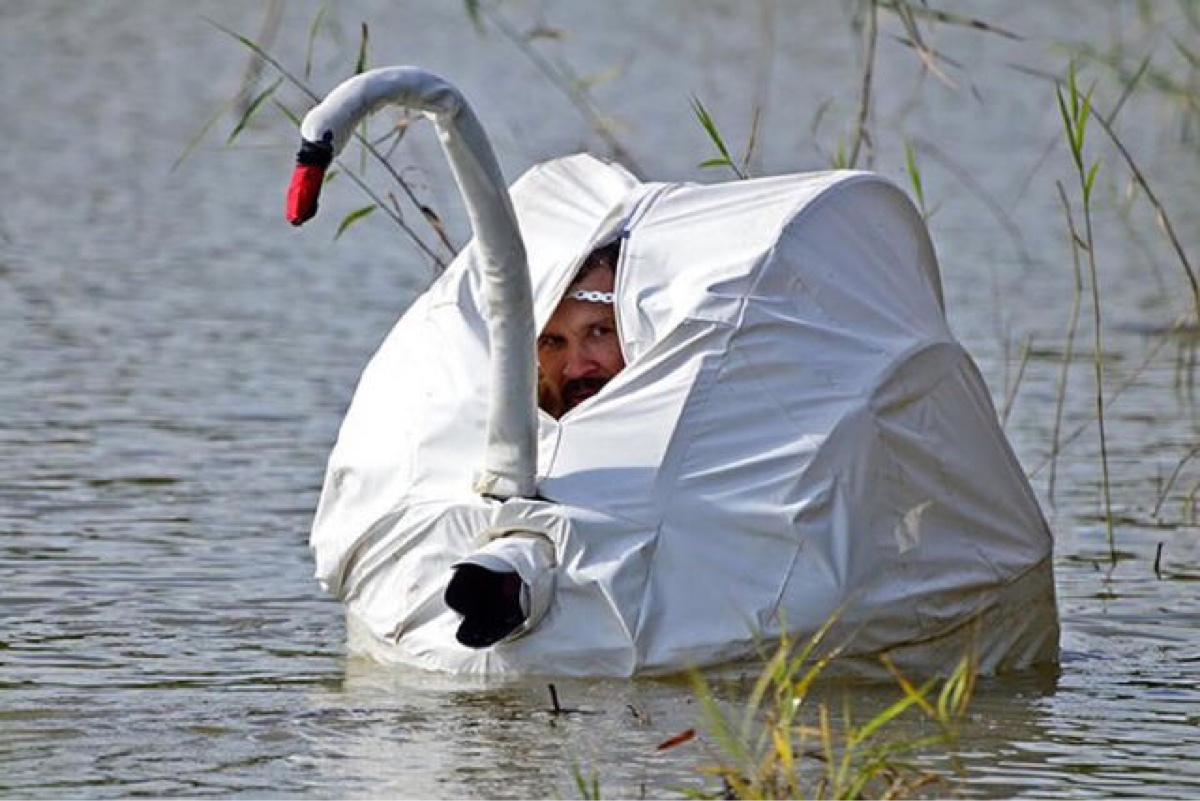
\includegraphics[width=0.9\textwidth]{Billeder/Redskaber/kunstigtskjul.jpg}
        \vspace{0.5cm}
        
    \end{columns}

\end{frame}


\section{Rovfugle (vildtkending og biologi)}

\begin{frame}
  \vspace{1.5em}
  \begin{center}
    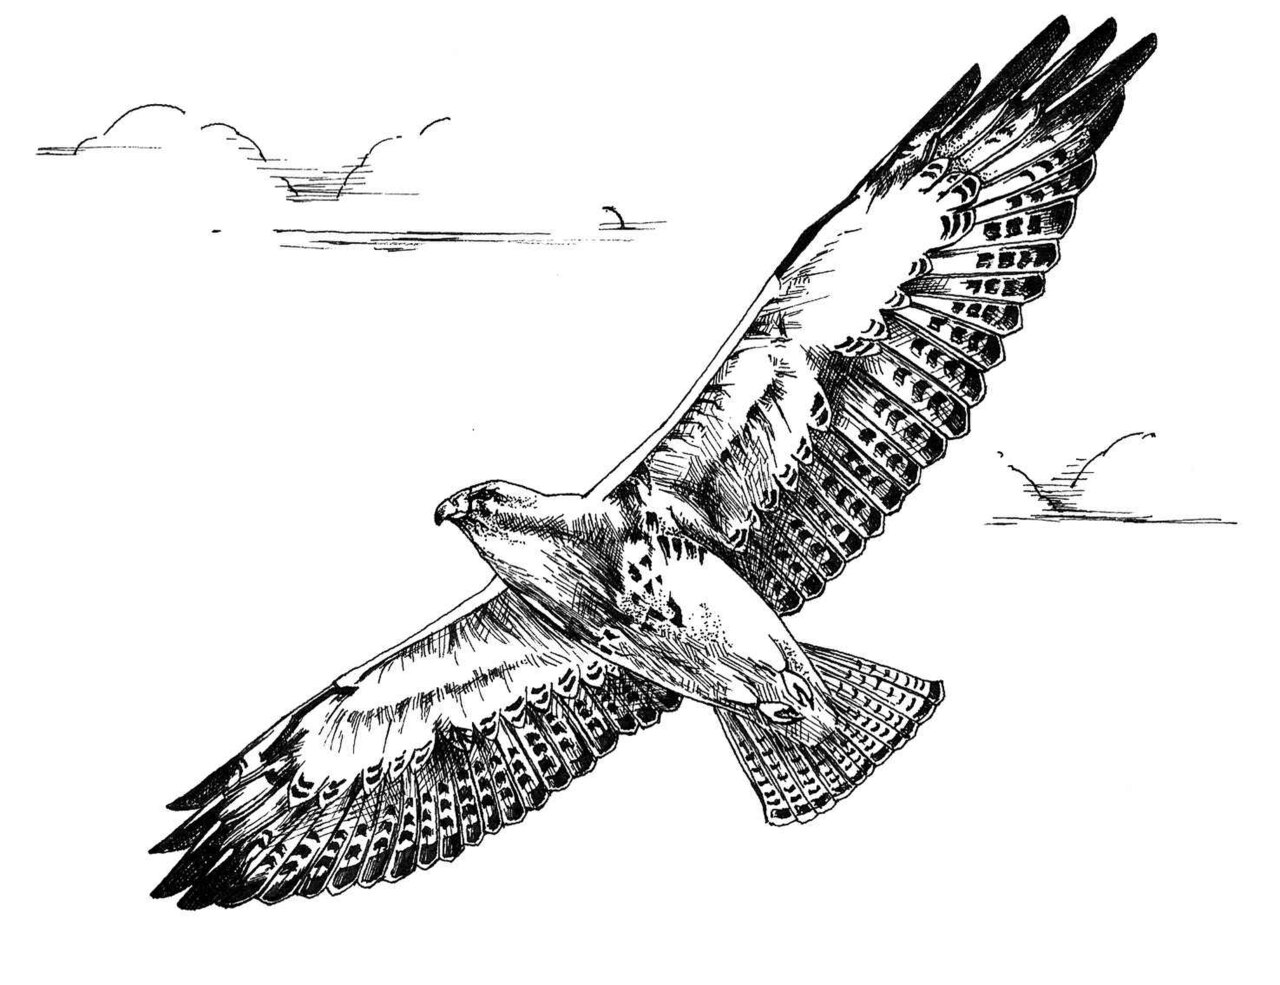
\includegraphics[width=12cm, height=4cm, keepaspectratio]{Billeder/Dyr/Fugle/Rovfugle/rovfugle.jpg}\\[1.2em]
    {\LARGE \textbf{Rovfugle}}
    \vspace{1em}
    \\ Artsbestemmelse og vildtbiologi
    \\[0.9em]
    {\tiny\color{gray}
    CC BY 4.0 – kan frit anvendes, også kommercielt. Rettighederne må ikke skærpes.\\[0.05em]
    Udviklet af Aleksander Sønder, OSJAGTTEGN.DK}
  \end{center}
\end{frame}

% ========== MUSVÅGE ==========
\begin{frame}{%
  \begin{minipage}[c]{0.30\textwidth}
    Musvåge
  \end{minipage}%
  \hfill
  \begin{minipage}[c]{0.45\textwidth}
    \footnotesize
    \textbf{Jagttid:} Ingen jagttid
  \end{minipage}%
  \hfill
  \begin{minipage}[c]{0.15\textwidth}
    \noindent\raggedleft
    
\includegraphics[width=0.5cm, height=0.5cm, keepaspectratio]{Billeder/Ikoner/star.png}%
    \hspace{0.2em}%
    
\includegraphics[width=0.5cm, height=0.5cm, keepaspectratio]{Billeder/Ikoner/star.png}
  \end{minipage}%
}
  \vspace{0.25em}
  \begin{columns}[T]
    % --- Venstre kolonne: Tekst ---
    \column{0.45\textwidth}
    \setlength{\parskip}{0.5em}
    \tiny
    \RaggedRight
    \textbf{\textit{Buteo buteo}} – kraftig bredskuldret rovfugl med musende kald \par
    \textbf{Udseende:}\\
    \quad – Brun men kan variere fra mørk til lys. Spraglet bryst. \par
    \textbf{Levesteder:} Det åbne land. \par
    \textbf{Føde:} Mus, gnavere, orme, frøer, harekillinger. \par
    \textbf{Udbredelse:} Hele Danmark. \par
    \textbf{Træk/standfugl:} Begge
    % --- Højre kolonne: Større billede ---
    \column{0.52\textwidth}
    \centering
    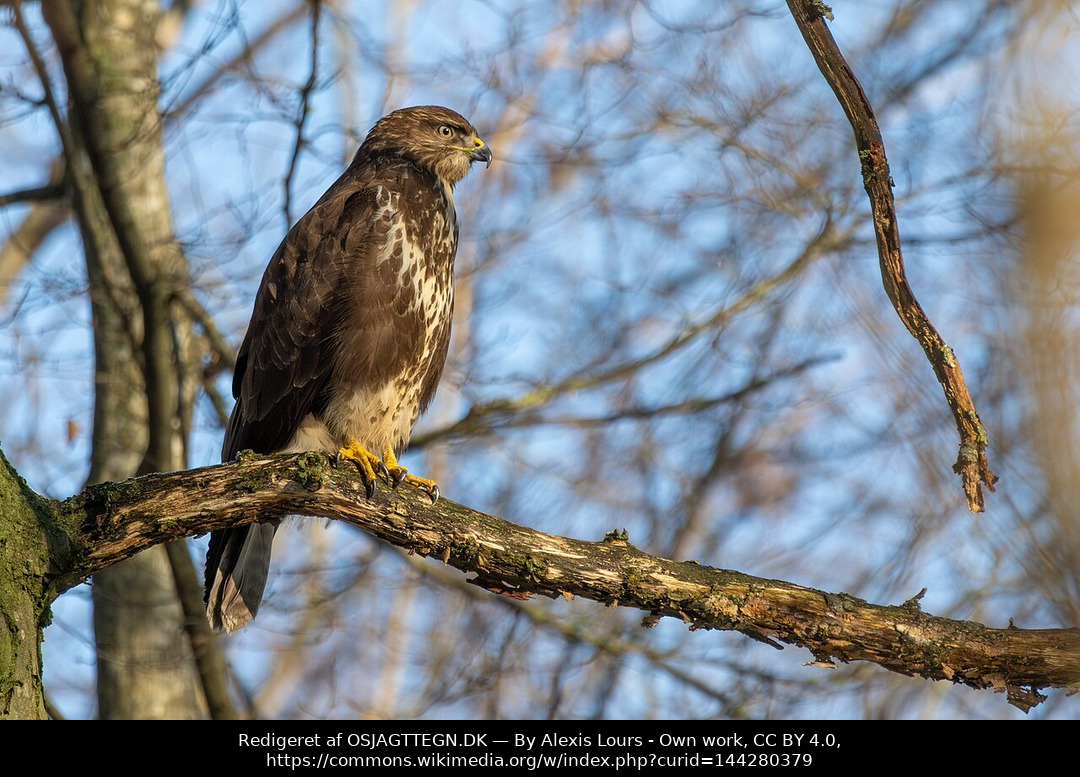
\includegraphics[width=\linewidth, height=7.2cm, keepaspectratio]{Billeder/Dyr/Fugle/Rovfugle/musvåge.jpg}
  \end{columns}
\end{frame}
% ========== SPURVEHØG ==========
\begin{frame}{%
  \begin{minipage}[c]{0.30\textwidth}
    Spurvehøg
  \end{minipage}%
  \hfill
  \begin{minipage}[c]{0.45\textwidth}
    \footnotesize
    \textbf{Jagttid:} Ingen jagttid
  \end{minipage}%
  \hfill
  \begin{minipage}[c]{0.15\textwidth}
    \noindent\raggedleft
    
\includegraphics[width=0.5cm, height=0.5cm, keepaspectratio]{Billeder/Ikoner/star.png}%
    \hspace{0.2em}%
    
\includegraphics[width=0.5cm, height=0.5cm, keepaspectratio]{Billeder/Ikoner/star.png}
  \end{minipage}%
}
  \vspace{0.25em}
  \begin{columns}[T]
    % --- Venstre kolonne: Tekst ---
    \column{0.45\textwidth}
    \setlength{\parskip}{0.5em}
    \tiny
    \RaggedRight
    \textbf{\textit{Accipiter nisus}} – relativt lille rovfugl \par
    \textbf{Udseende:}\\
    \quad – Tynde gule tændstiksben, rustrøde tværstriber på bryst \par
    \textbf{Levesteder:} Skovområder men forefindes også i byområder. \par
    \textbf{Føde:} Spurve og drosler som fanges ved overraskelse. \par
    \textbf{Udbredelse:} Hele Danmark. \par
    \textbf{Træk/standfugl:} Begge
    % --- Højre kolonne: Større billede ---
    \column{0.52\textwidth}
    \centering
    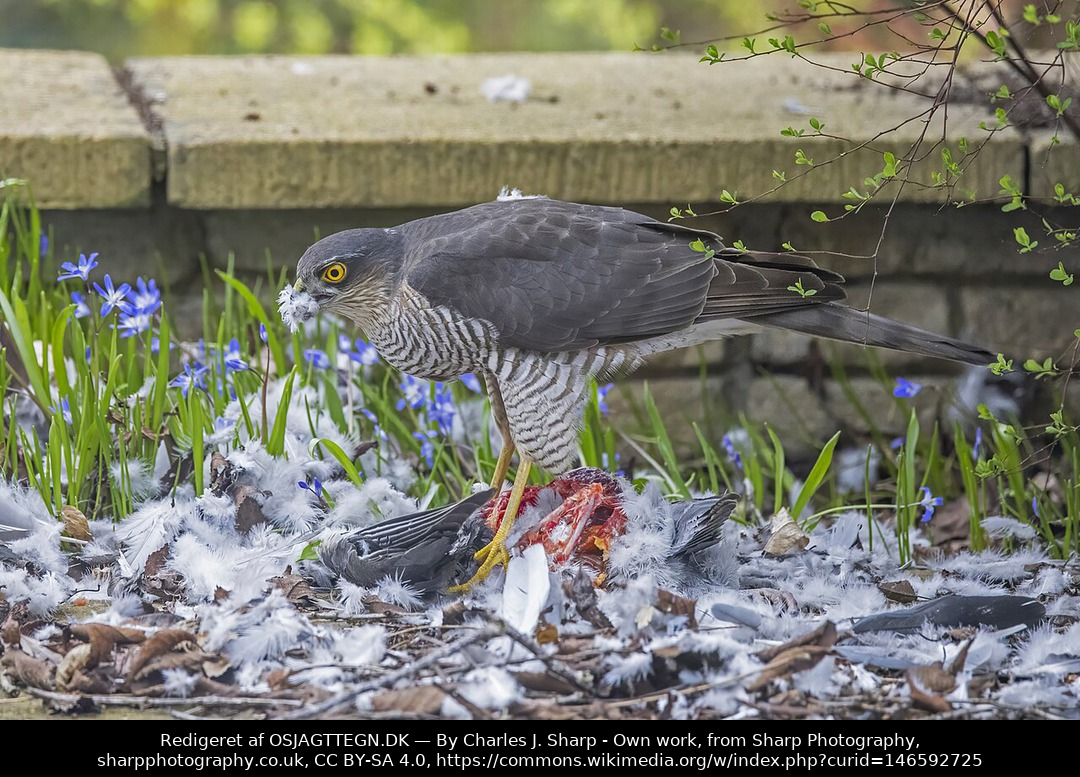
\includegraphics[width=\linewidth, height=7.2cm, keepaspectratio]{Billeder/Dyr/Fugle/Rovfugle/spurvehøg.jpg}
  \end{columns}
\end{frame}
% ========== TÅRNFALK ==========
\begin{frame}{%
  \begin{minipage}[c]{0.30\textwidth}
    Tårnfalk
  \end{minipage}%
  \hfill
  \begin{minipage}[c]{0.45\textwidth}
    \footnotesize
    \textbf{Jagttid:} Ingen jagttid
  \end{minipage}%
  \hfill
  \begin{minipage}[c]{0.15\textwidth}
    \noindent\raggedleft
    
\includegraphics[width=0.5cm, height=0.5cm, keepaspectratio]{Billeder/Ikoner/star.png}%
    \hspace{0.2em}%
    
\includegraphics[width=0.5cm, height=0.5cm, keepaspectratio]{Billeder/Ikoner/star.png}
  \end{minipage}%
}
  \vspace{0.25em}
  \begin{columns}[T]
    % --- Venstre kolonne: Tekst ---
    \column{0.45\textwidth}
    \setlength{\parskip}{0.5em}
    \tiny
    \RaggedRight
    \textbf{\textit{Falco tinnunculus}} – en af de mest udbredte rovfugle i Danmark \par
    \textbf{Udseende:}\\
    \quad – Teglrød overside med pletter, mørke tværbånd på halen \par
    \textbf{Levesteder:} Åbne arealer, også i byer og langs veje. \par
    \textbf{Føde:} Mus, gnavere og insekter. \par
    \textbf{Udbredelse:} Hele Danmark. \par
    \textbf{Træk/standfugl:} Begge
    % --- Højre kolonne: Større billede ---
    \column{0.52\textwidth}
    \centering
    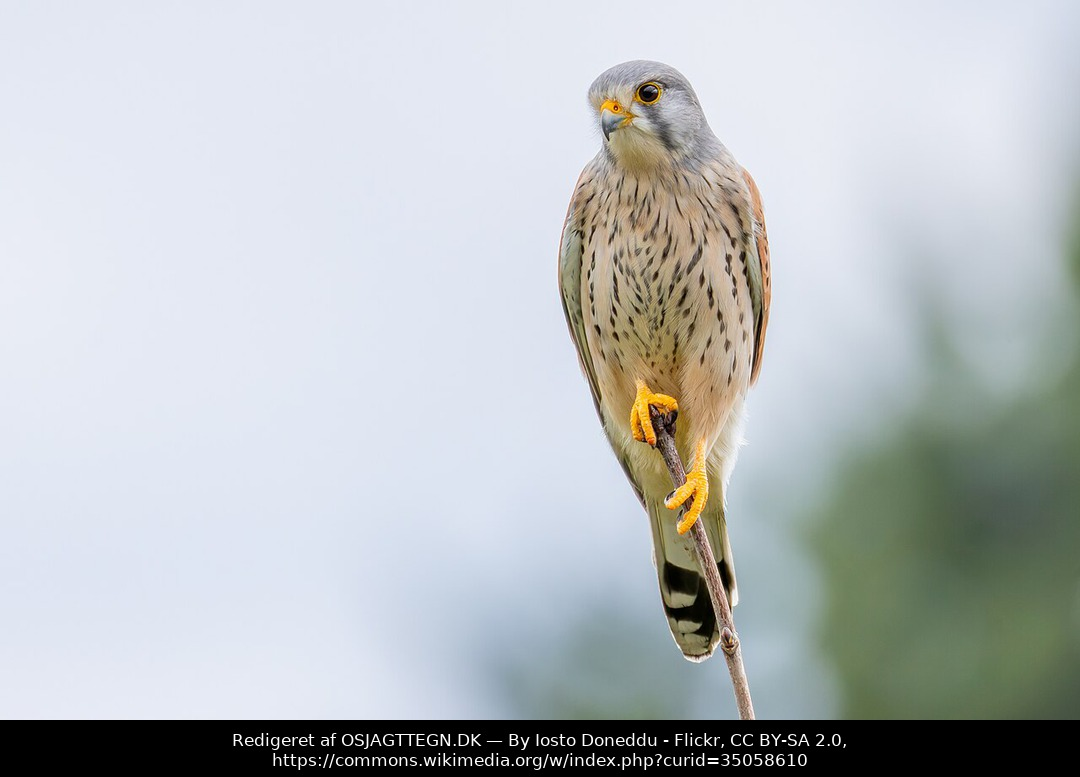
\includegraphics[width=\linewidth, height=7.2cm, keepaspectratio]{Billeder/Dyr/Fugle/Rovfugle/tårnfalk.jpg}
  \end{columns}
\end{frame}
% ========== DUEHØG ==========
\begin{frame}{%
  \begin{minipage}[c]{0.30\textwidth}
    Duehøg
  \end{minipage}%
  \hfill
  \begin{minipage}[c]{0.45\textwidth}
    \footnotesize
    \textbf{Jagttid:} Ingen jagttid
  \end{minipage}%
  \hfill
  \begin{minipage}[c]{0.15\textwidth}
    \noindent\raggedleft
    
\includegraphics[width=0.5cm, height=0.5cm, keepaspectratio]{Billeder/Ikoner/star.png}
  \end{minipage}%
}
  \vspace{0.25em}
  \begin{columns}[T]
    % --- Venstre kolonne: Tekst ---
    \column{0.45\textwidth}
    \setlength{\parskip}{0.5em}
    \tiny
    \RaggedRight
    \textbf{\textit{Accipiter gentilis}} – stor høg \par
    \textbf{Udseende:}\\
    \quad – Grå, med tværtstriber på bryst, lys øjenstribe
    % --- Højre kolonne: Større billede ---
    \column{0.52\textwidth}
    \centering
    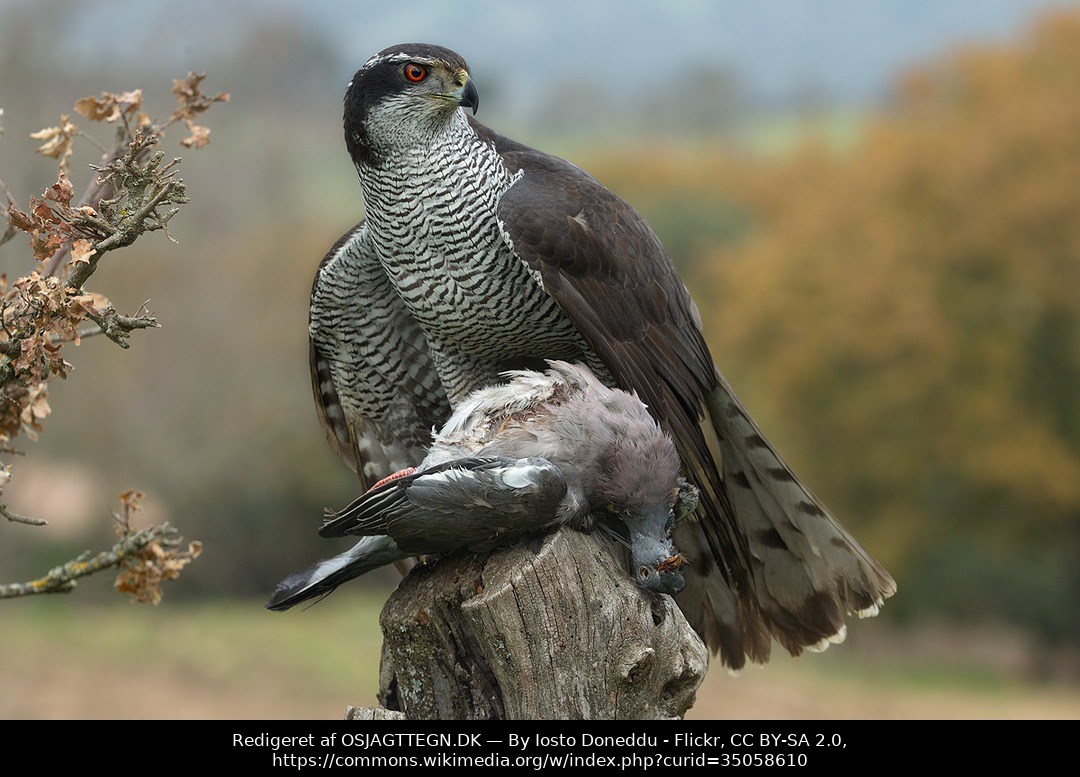
\includegraphics[width=\linewidth, height=7.2cm, keepaspectratio]{Billeder/Dyr/Fugle/Rovfugle/duehoeg.jpg}
  \end{columns}
\end{frame}
% ========== VANDREFALK ==========
\begin{frame}{%
  \begin{minipage}[c]{0.30\textwidth}
    Vandrefalk
  \end{minipage}%
  \hfill
  \begin{minipage}[c]{0.45\textwidth}
    \footnotesize
    \textbf{Jagttid:} Ingen jagttid
  \end{minipage}%
  \hfill
  \begin{minipage}[c]{0.15\textwidth}
    \noindent\raggedleft
    
\includegraphics[width=0.5cm, height=0.5cm, keepaspectratio]{Billeder/Ikoner/star.png}
  \end{minipage}%
}
  \vspace{0.25em}
  \begin{columns}[T]
    % --- Venstre kolonne: Tekst ---
    \column{0.45\textwidth}
    \setlength{\parskip}{0.5em}
    \tiny
    \RaggedRight
    \textbf{\textit{Falco peregrinus}} – mellemstor falk – kan flyve 150 km/t \par
    \textbf{Udseende:}\\
    \quad – Tynde tværstriber med sort pilothjelm. Bemærk skægstriben
    % --- Højre kolonne: Større billede ---
    \column{0.52\textwidth}
    \centering
    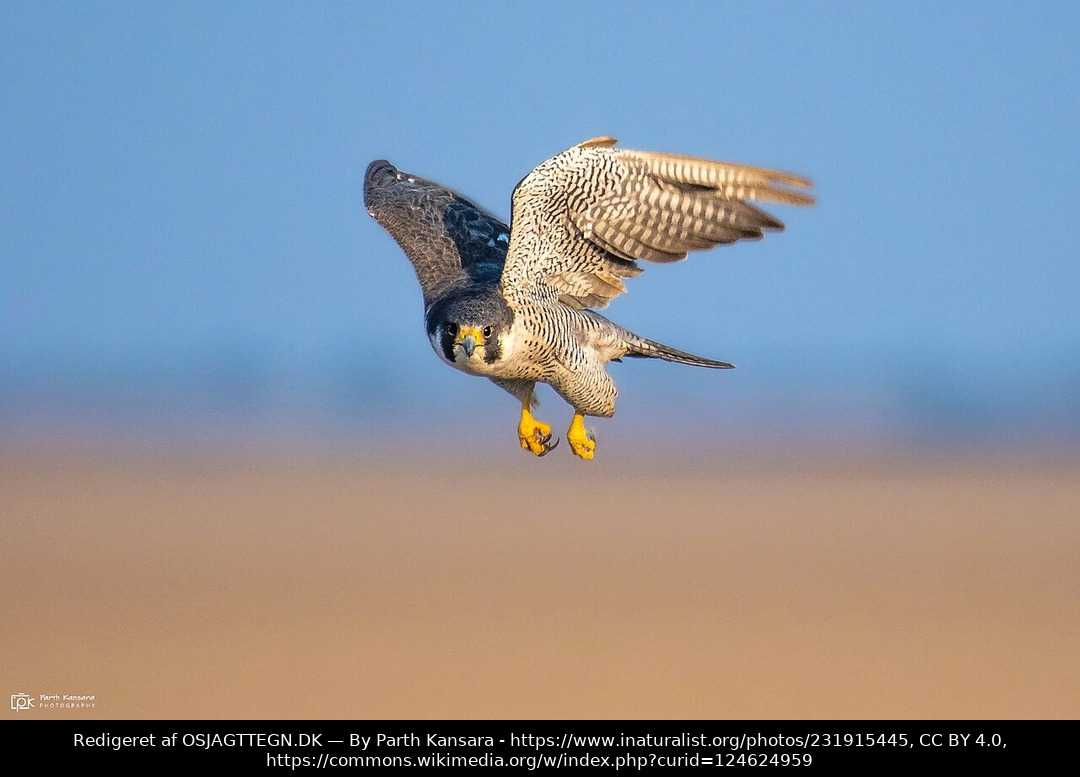
\includegraphics[width=\linewidth, height=7.2cm, keepaspectratio]{Billeder/Dyr/Fugle/Rovfugle/vandrefalk.jpg}
  \end{columns}
\end{frame}
% ========== RØRHØG ==========
\begin{frame}{%
  \begin{minipage}[c]{0.30\textwidth}
    Rørhøg
  \end{minipage}%
  \hfill
  \begin{minipage}[c]{0.45\textwidth}
    \footnotesize
    \textbf{Jagttid:} Ingen jagttid
  \end{minipage}%
  \hfill
  \begin{minipage}[c]{0.15\textwidth}
    \noindent\raggedleft
    
\includegraphics[width=0.5cm, height=0.5cm, keepaspectratio]{Billeder/Ikoner/star.png}
  \end{minipage}%
}
  \vspace{0.25em}
  \begin{columns}[T]
    % --- Venstre kolonne: Tekst ---
    \column{0.45\textwidth}
    \setlength{\parskip}{0.5em}
    \tiny
    \RaggedRight
    \textbf{\textit{Circus aeruginosus}} – i familien kærhøge som er kendetegnet ved v-formen i vingerne \par
    \textbf{Udseende:}\\
    \quad – Flødegult hovede og bryst, lange ben
    % --- Højre kolonne: Større billede ---
    \column{0.52\textwidth}
    \centering
    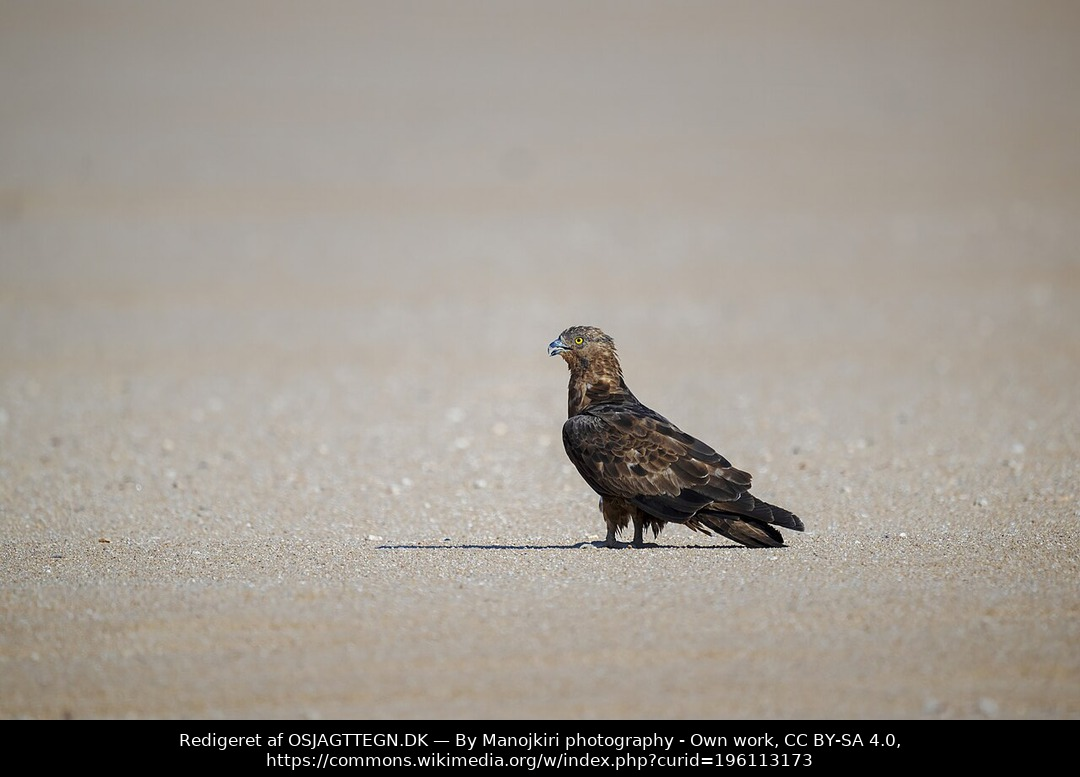
\includegraphics[width=\linewidth, height=7.2cm, keepaspectratio]{Billeder/Dyr/Fugle/Rovfugle/rørhøg.jpg}
  \end{columns}
\end{frame}
% ========== FISKEØRN ==========
\begin{frame}{%
  \begin{minipage}[c]{0.30\textwidth}
    Fiskeørn
  \end{minipage}%
  \hfill
  \begin{minipage}[c]{0.45\textwidth}
    \footnotesize
    \textbf{Jagttid:} Ingen jagttid
  \end{minipage}%
  \hfill
  \begin{minipage}[c]{0.15\textwidth}
    \noindent\raggedleft
    
\includegraphics[width=0.5cm, height=0.5cm, keepaspectratio]{Billeder/Ikoner/star.png}
  \end{minipage}%
}
  \vspace{0.25em}
  \begin{columns}[T]
    % --- Venstre kolonne: Tekst ---
    \column{0.45\textwidth}
    \setlength{\parskip}{0.5em}
    \tiny
    \RaggedRight
    \textbf{\textit{Pandion haliaetus}} – mellemstor rovfugl med lange smalle vinger \par
    \textbf{Udseende:}\\
    \quad – Grå overside, hvid underside. Hvidt hoved med sort stribe langsgående med halsen. Blå ben
    % --- Højre kolonne: Større billede ---
    \column{0.52\textwidth}
    \centering
    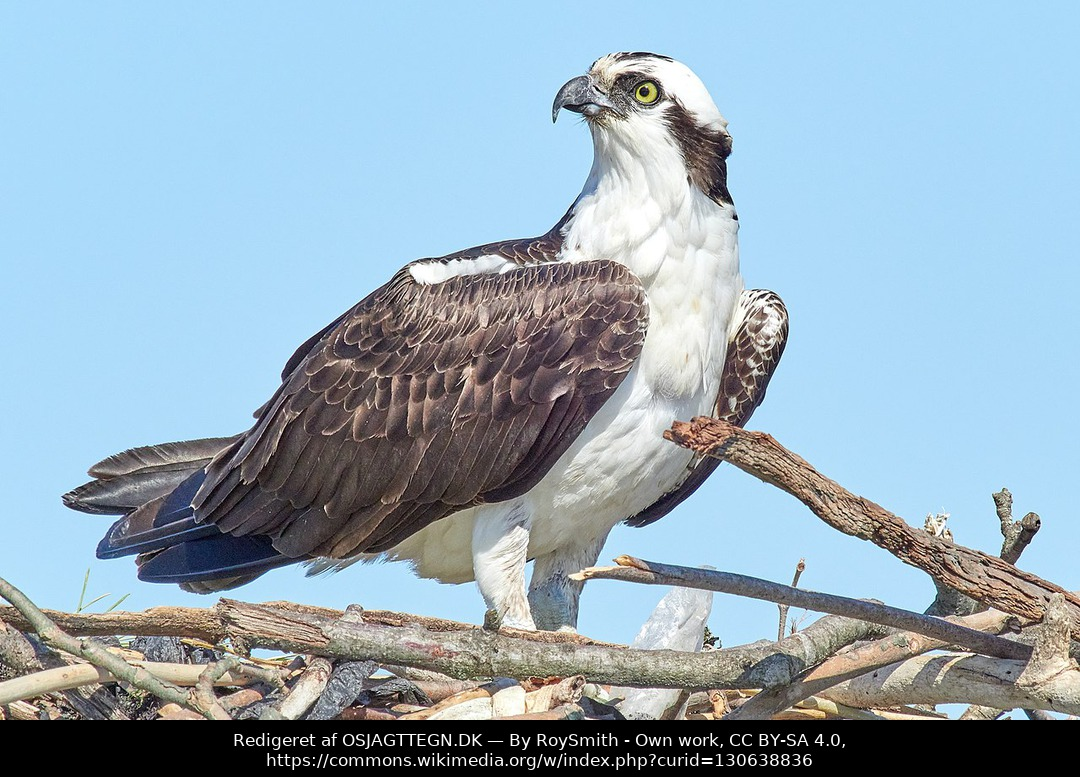
\includegraphics[width=\linewidth, height=7.2cm, keepaspectratio]{Billeder/Dyr/Fugle/Rovfugle/fiskeørn.jpg}
  \end{columns}
\end{frame}

\section{Afstandsbedømmelse - Praktisk del af jagtprøven)}

\begin{frame}
  \vspace{1.5em}
  \begin{center}
    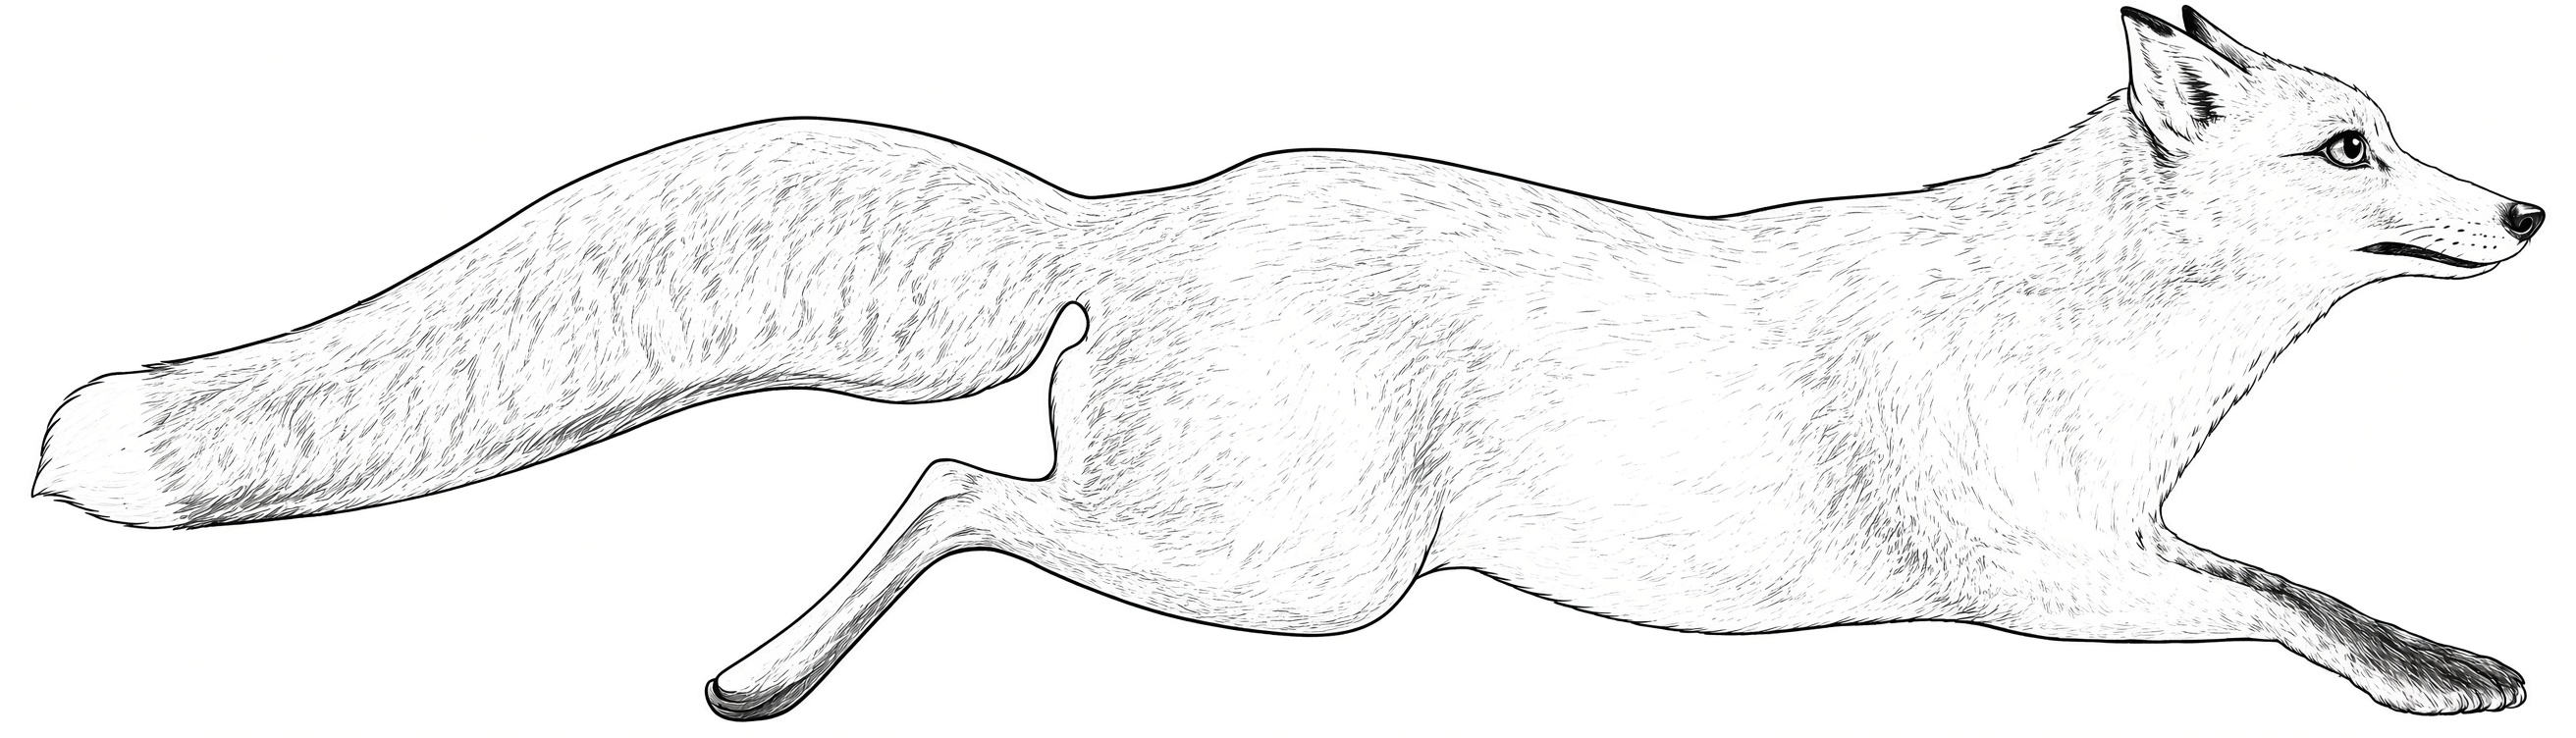
\includegraphics[width=12cm, height=2cm, keepaspectratio]{Billeder/Andet/Afstandsbedømmelse/afstandsbedømmelse.jpg}\\[1.2em]
    {\LARGE \textbf{Afstandsbedømmelse}}
    \vspace{1em}
    \\ En del af jagtprøven
    \\[0.9em]
    {\tiny\color{gray}
    CC BY 4.0 – kan frit anvendes, også kommercielt. Rettighederne må ikke skærpes.\\[0.05em]
    Udviklet af Aleksander Sønder, OSJAGTTEGN.DK}
  \end{center}
\end{frame}

% ========== AFSTANDSVURDERING ==========
\begin{frame}{Afstandsbedømmelse struktur}
  \tiny
  \setlength{\parskip}{0.35em}
  \RaggedRight

  \textbf{Sådan foregår afstandsbedømmelse}
  \begin{itemize}
    \itemsep0.15em
    \item Aspiranten skal vurdere afstanden ved \textbf{4 forskellige punkter}.
    \item Ved hvert punkt står \textbf{1 eller 2 vildtfigurer} efter den valgte afstandsserie.
    \item Der spørges om \textbf{1 figur ad gangen}.
    \item Figuren udpeges, og der spørges: \textit{``Er skudafstanden forsvarlig til \ldots?''}
    \item Herefter starter tidtagningen. Svarfristen er \textbf{5 sekunder}.
    \item Klart svar: enten JA el. NEJ \textbf{fejl}.
    \item Svar efter tiden tæller som \textbf{fejl}.
    \item Efter hvert punkt får aspiranten at vide, om svaret var korrekt.
  \end{itemize}

  \textbf{Krav til opstilling}
  \begin{itemize}
    \itemsep0.15em
    \item Punkterne placeres hensigtsmæssigt på den enkelte bane.
    \item Der må \textbf{ikke} bruges faste baner, så forløbet kan forudses.
    \item Mindst \textbf{1 fuglefigur} skal være hævet \textbf{2--4 m} over aspirantens niveau og så vidt muligt med himlen som baggrund.
    \item Samme afstandsserie bruges til samme prøvehold.
    \item Ved mistanke om snyd sættes en \textbf{ny serie} op.
    \item Afstandene skal måles før hver prøvedag med båndmål, målehjul eller laser.
  \end{itemize}

  \vspace{0.3em}
  \textbf{Beståkrav:} 5 ud af 6 afstande skal besvares korrekt.
\end{frame}

% ========== VILDTFIGURER: MAX OG PLACERING ==========
\begin{frame}{Vildtfigurer system, 3 klasser og 5 afstande}
  \vspace{-0.3em}
  \centering
  \scriptsize
  \setlength{\tabcolsep}{5pt}
  \renewcommand{\arraystretch}{1.25}

  \begin{tabular}{l c c l l}
    \toprule
    \textbf{Art} & \textbf{Billede} & \textbf{Max} & \textbf{Korrekt} & \textbf{Forkert} \\
    \midrule
    Gråand
      & 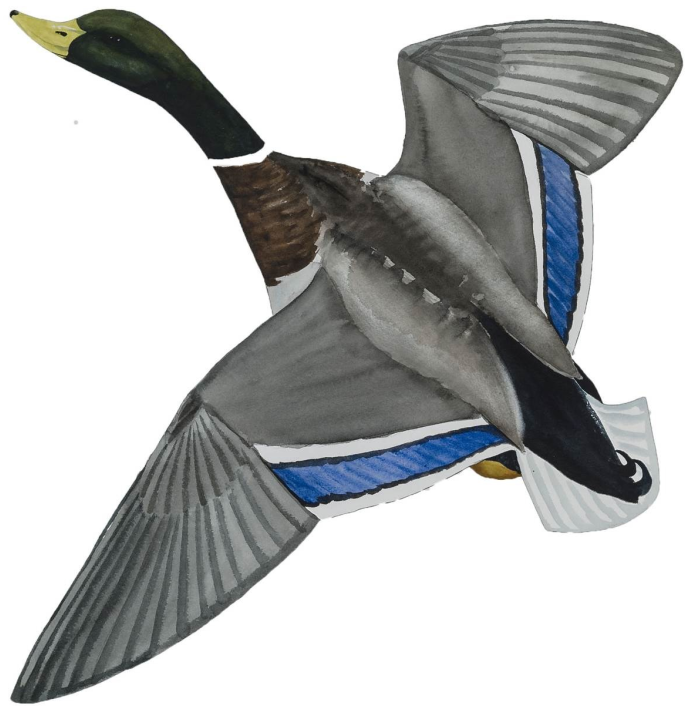
\includegraphics[height=0.9cm]{Billeder/Andet/Afstandsbedømmelse/gråand.png}
      & 30 m
      & 26 m (JA)
      & 38 m (NEJ) \\
    Hare
      & 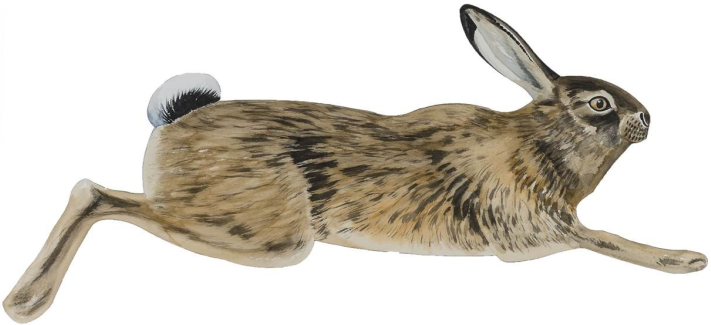
\includegraphics[height=0.9cm]{Billeder/Andet/Afstandsbedømmelse/hare.png}
      & 30 m
      & 26 m (JA)
      & 38 m (NEJ) \\
    Fasan
      & 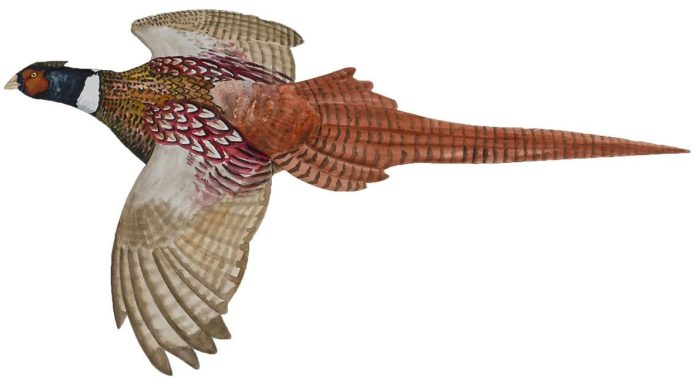
\includegraphics[height=0.9cm]{Billeder/Andet/Afstandsbedømmelse/fasan.png}
      & 30 m
      & 26 m (JA)
      & 38 m (NEJ) \\
    Ræv
      & 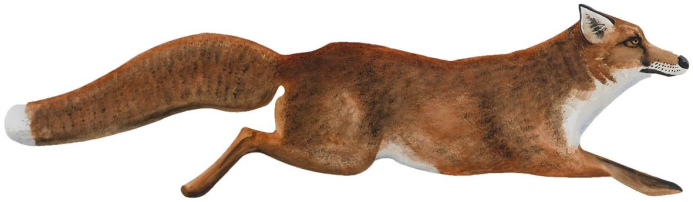
\includegraphics[height=0.9cm]{Billeder/Andet/Afstandsbedømmelse/ræv.png}
      & 25 m
      & 22 m (JA)
      & 32 m (NEJ) \\
    Grågås
      & 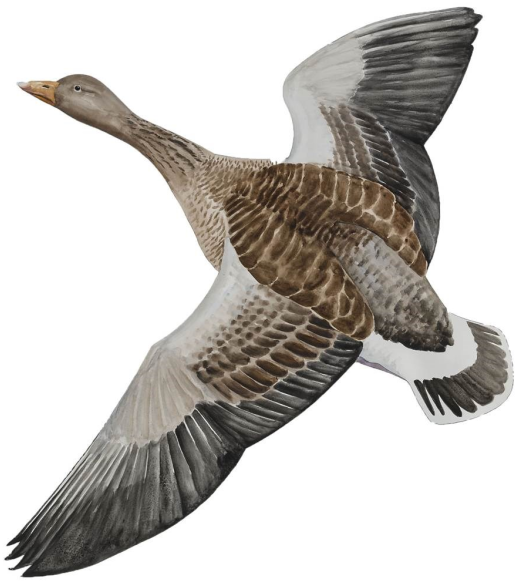
\includegraphics[height=0.9cm]{Billeder/Andet/Afstandsbedømmelse/grågås.png}
      & 25 m
      & 22 m (JA)
      & 32 m (NEJ) \\
    Råvildt
      & 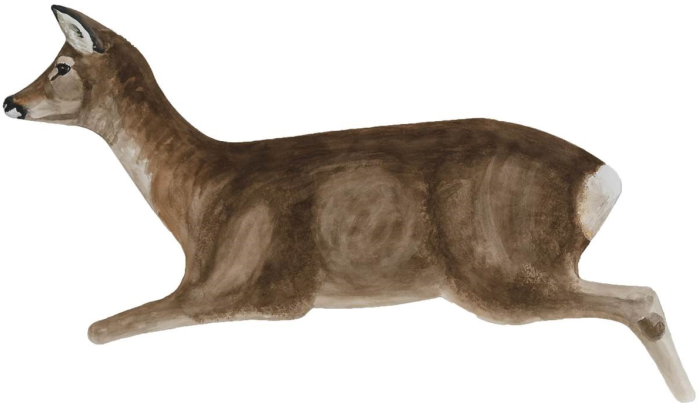
\includegraphics[height=0.9cm]{Billeder/Andet/Afstandsbedømmelse/råvildt.png}
      & 20 m
      & 17 m (JA)
      & 26 m (NEJ) \\
    \bottomrule
  \end{tabular}

  \vspace{0.8em}
  \tiny
  \textbf{JA} = inden for teoretisk max-skydeafstand \quad
  \textbf{NEJ} = længere end teoretisk max-skydeafstand
\end{frame}



% ========== SERIEPUNKTER ==========
\begin{frame}{Forskellige serier}
  \vspace{0.3em}
  \centering
  \footnotesize
  \begin{tabular}{lcccccccc}
    \toprule
    \textbf{Serie} & \textbf{1} & \textbf{2} & \textbf{3} & \textbf{4} & \textbf{5} & \textbf{6} & \textbf{7} & \textbf{8} \\
    \midrule
    Gråand (max.\ 30)   & 26 & 38 & 26 & 38 & 26 & 38 & 26 & 38 \\
    Ræv (max.\ 25)      & 22 & 32 & 22 & 32 & 22 & 32 & 22 & 32 \\
    Hare (max.\ 30)     & 26 & 26 & 26 & 26 & 38 & 38 & 38 & 38 \\
    Råvildt (max.\ 20)  & 17 & 17 & 26 & 26 & 17 & 17 & 26 & 17 \\
    Fasan (max.\ 30)    & 38 & 26 & 38 & 38 & 38 & 26 & 38 & 26 \\
    Grågås (max.\ 25)   & 32 & 22 & 32 & 22 & 22 & 32 & 32 & 22 \\
    \bottomrule
  \end{tabular}
\end{frame}

\section{Jagtudøvelse}

\begin{frame}
  \vspace{3em}
  \begin{center}
    {\LARGE \textbf{Bekendtgørelse af lov om jagt og vildtforvaltning}} \\
    \vspace{1em}
    LBK nr 639 af 26/05/2023, §§ 13-32
  \end{center}
\end{frame}

\begin{frame}{Jagtretten – grundregler (§13–§15)}
    \begin{itemize}
        \item \textbf{§13}: Ingen må jage uden jagtret – medmindre samtykke fra jagtberettiget
        \item \textbf{§14}: Jagtretten tilkommer ejendommens ejer
          \begin{itemize}
            \item På ferske vande (uden særlig ejendomsret): Ejerne af tilstødende ejendomme (nærmeste del)
            \item Gælder ikke hvis ældre rettigheder giver retten til andre
          \end{itemize}
        \item \textbf{§15}: Fast bopæl i DK → ret til ikke-erhvervsmæssig jagt på fiskeriterritoriet (fra højeste vandstandslinje)
          \begin{itemize}
            \item Gælder ikke hvis ældre ret til tilgrænsende landarealer
            \item Undtagelse: EU/EØS-borgere med tilknytning til DK
          \end{itemize}
    \end{itemize}
\end{frame}

\begin{frame}{Jagtretten – offentlig vej og tilegnelse (§16–§17)}
    \begin{itemize}
        \item \textbf{§16}: Forbud mod jagt på/fra offentlig vej eller sti
          \begin{itemize}
            \item Tilladt at tilegne sig beskudt vildt, der falder på vej/sti fra egen grund
          \end{itemize}
        \item \textbf{§17}: Beskudt vildt på egen grund → må ikke tilegnes hvis det falder på anden grund
          \begin{itemize}
            \item Underret snarest ejer/jagtberettiget
          \end{itemize}
    \end{itemize}
\end{frame}

\begin{frame}{Arealgrænser og minimumskrav (§18)}
    \begin{itemize}
        \item \textbf{§18}: Minimum 1 ha sammenhængende areal til jagt (vej/jernbane krydses OK)
          \begin{itemize}
            \item Fra 1 - 5 ha: Kun ejer + husstand (eller brugsret-indehaver + husstand)
            \item Aftale med tilgrænsende arealer → kan overstige grænser (naboaftale)
            \item Øer mindre end 1 ha: OK hvis jagt tilladt på omgivende fiskeriterritorium
            \item Fælleseje (flere end 4 ejere): Skriftlig aftale + 3/4 tilslutning
          \end{itemize}
    \end{itemize}
\end{frame}


\begin{frame}{Afstande, overdragelse og ældre rettigheder (§19–§21)}
    \begin{itemize}
        \item \textbf{§19}: Ingen skud inden for 50 m fra beboelsesbygninger (uden samtykke)
          \begin{itemize}
            \item På fiskeriterritoriet: 100 m fra sommerhusområde / 500 m fra byzone
          \end{itemize}
        \item \textbf{§20}: Jagtretten kan ikke afhændes særskilt/varigt fra ejendomsretten
          \begin{itemize}
            \item Overdragelse: Max 30 år ad gangen
            \item Ved brugsret-overdragelse: Jagtretten følger med (medmindre aftalt andet)
          \end{itemize}
        \item \textbf{§21}: Ældre rettigheder → ejer kan kræve afløsning (kapitaliseret jagtleje)
    \end{itemize}
\end{frame}



\begin{frame}{Jagtetik, sikkerhed og unge jægere (§22–§23)}
    \begin{itemize}
        \item \textbf{§22}: Ingen må jage på en måde, der
          \begin{itemize}
            \item udsætter vildtet for unødige lidelser
            \item skader personer, husdyr eller genstande eller udsætter personer for nærliggende fare
            \item medfører haglnedfald på anden persons bolig, have eller gårdsplads
          \end{itemize}
        \item \textbf{Stk. 2}: Personer under 18 år (med gyldigt jagttegn) må kun jage i følge med en person over 18 år (med gyldigt jagttegn)
        \item \textbf{§23}: Nedlæggelse/ombringelse af vildt må kun ske med skydevåben
          \begin{itemize}
            \item Rovfugle og ugler må ikke anvendes til jagt
            \item Jagt må ikke ske med levende lokkedyr
          \end{itemize}
    \end{itemize}
\end{frame}

\begin{frame}{Våbenkrav, hunde og jagt fra køretøj/fartøj (§24–§26)}
    \begin{itemize}
        \item \textbf{§24}: Ved jagt med glatløbet haglgevær på ikkeklovbærende vildt (på/fra landarealer, rør- og sivbevoksninger) skal egnet apporterende hund medbringes
        \item \textbf{§25}: Jagt må ikke finde sted fra motordrevet køretøj eller luftfartøj
        \item \textbf{§26}: Jagt fra motordrevet fartøj må ikke finde sted på søer og andre ferske vande
        \item \textbf{§23 stk. 4–6}: Ministeren fastsætter regler om
          \begin{itemize}
            \item tilladte våben/ammunition
            \item salg/medtagelse af visse ammunitionstyper
            \item brug af rovfugle, hjælpemidler, lokkemidler mv.
          \end{itemize}
    \end{itemize}
\end{frame}

\begin{frame}{Fodring, skjul, hegn og færdsel med våben (§28–§31)}
    \begin{itemize}
        \item \textbf{§28}: Udfodring af vildt med jagt for øje må ikke finde sted – vildt må ikke beskydes nær foderplads
          \begin{itemize}
            \item Ministeren kan fastsætte regler om fodring, foderpladser og placering
          \end{itemize}
        \item \textbf{§29}: Ministeren kan fastsætte regler om jagt fra platforme/kunstige skjul (inkl. forbud mod at medtage våben)
        \item \textbf{§30}: Hegn skal tillade ens passage af vildt fra begge sider (undtaget udsætningspladser, skovkulturer, veje/jernbaner)
        \item \textbf{§31}: Uvedkommende må ikke færdes med skydevåben/fangstredskaber på anden persons jagtgrund (undt. offentlige veje/stier)
          \begin{itemize}
            \item Gælder også i skove – kun på offentlige veje gennem skoven
            \item Naturbeskyttelseslovens adgangsregler giver ikke ret til at medbringe skydevåben/fangstredskaber
          \end{itemize}
    \end{itemize}
\end{frame}

\begin{frame}{Særlige jagtformer og anholdelsesbeføjelser (§27, §32)}
    \begin{itemize}
        \item \textbf{§27}: Ministeren kan fastsætte regler om jagtformer (herunder forbyde særlige former i bestemte områder)
        \item \textbf{§32}: Den jagtberettigede (eller dennes folk) må anholde enhver, der overtræder §13 (ulovlig jagt uden ret)
          \begin{itemize}
            \item Må føre den anholdte til politiet
            \item Samme beføjelse til arealet brugeren (selv uden jagtret) – skal underrette jagtberettiget
            \item Anholdte kan fratages skydevåben, redskaber og skudt/fanget vildt – afleveres straks til politiet (beslaglæggelse vurderes)
          \end{itemize}
    \end{itemize}
\end{frame}

\begin{frame}
  \vspace{3em}
  \begin{center}
    {\LARGE \textbf{Jagtudøvelse}
    }
    \\
    \vspace{1em}
    Bekendtgørelse om udsætning af vildt, jagtmåder og jagtredskaber
    \\
    \vspace{1em}
    BEK nr 1652 af 19/12/2017, Kapitel 2-5
  \end{center}
\end{frame}

\begin{frame}{Jagt i nærheden af indhegninger med hjorte (§4–§5)}
    \begin{itemize}
        \item \textbf{§4}: På ejendom med indhegnet hold af hjortedyr (jf. lov om hold af dyr)
          \begin{itemize}
            \item Vildtlevende individer af de opdrættede arter må \textbf{ikke} jages
            \item Gælder \textbf{i indhegningen} eller inden for \textbf{300 m} fra indhegningen
            \item Gælder også indhegninger, der er undtaget helt/delvist fra lov om hold af dyr (§19)
          \end{itemize}
        \item \textbf{§5}: På ejendom, hvor der \textbf{tidligere} har været holdt hjortedyr i indhegninger
          \begin{itemize}
            \item Hjortedyr må \textbf{ikke} jages \textbf{i indhegningen}
            \item Gælder hvis indhegningen (eller væsentlige dele) fortsat findes
          \end{itemize}
    \end{itemize}
\end{frame}



\begin{frame}{Jagt på fiskeriterritoriet – grundregler (§6)}
    \begin{itemize}
        \item \textbf{§6 stk. 1}: Den frie jagtret (jf. lovens §15) må kun udøves
          \begin{itemize}
            \item Fra flydende båd eller pram
            \item Fra areal, der grænser op til fiskeriterritoriet, hvor man har jagtret
          \end{itemize}
        \item \textbf{Stk. 2}: Færdsel med skydevåben under vadning på fiskeriterritoriet er \textbf{ikke tilladt}
        \item \textbf{Stk. 3} – Undtagelser (uanset stk. 1):
          \begin{itemize}
            \item Lovligt nedlagt vildt må indsamles ved vadning
            \item Rør- og sivbevoksninger må afdrives for vildt af den, der har jagtret på nærmeste tilgrænsende areal
          \end{itemize}
        \item \textbf{Stk. 4} – Vadning med skydevåben tilladt hvis:
          \begin{itemize}
            \item Skydevåbnet er \textbf{uladt}
            \item Vadning sker til/fra fartøj, ø eller holm med jagtret
            \item Ad korteste vej til sted, hvor våben lovligt kan medbringes (jf. §31)
          \end{itemize}
    \end{itemize}
\end{frame}

\begin{frame}{Fiskeriterritoriet}
    \begin{center}
        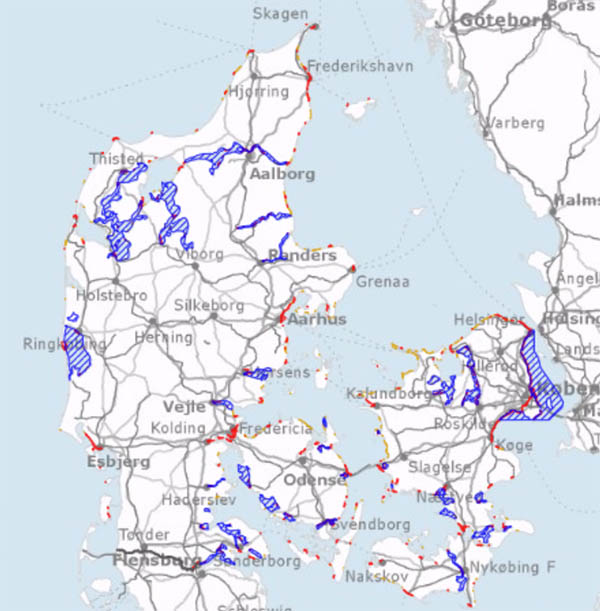
\includegraphics[width=0.45\textwidth]{Billeder/Andet/reservatkort.jpg}
        % Eller: [height=0.6\textheight] for højde-baseret skalering
    \end{center}
    
    % Her kan du tilføje tekst under billedet
    \vspace{1em}
    
\end{frame}

\begin{frame}{Jagt på fiskeriterritoriet – is og særlige begrænsninger (§7)}
    \begin{itemize}
        \item \textbf{§7 stk. 1}: På fiskeriterritoriet må der \textbf{ikke} drives jagt
          \begin{itemize}
            \item Fra is
            \item Inden for 100 m fra iskant
          \end{itemize}
        \item \textbf{Stk. 2}: Reglen i stk. 1 gælder \textbf{ikke} for jagt på \textbf{ræv}
    \end{itemize}
\end{frame}



\begin{frame}{Jagt fra båd – forbud og begrænsninger (§8)}
    \begin{itemize}
        \item \textbf{§8 stk. 1}: Der må \textbf{ikke} drives jagt fra motordrevet fartøj \textbf{i september måned}
        \item \textbf{Stk. 2}: Der må \textbf{ikke} drives jagt fra motordrevet fartøj
          \begin{itemize}
            \item på søer og andre ferske vande
            \item på de dele af fiskeriterritoriet, der er nævnt i \textbf{bilag 1} til bekendtgørelsen (vist på kortbilag)
          \end{itemize}
        \item \textbf{Stk. 3}: Der må \textbf{ikke} sejles med \textbf{ladt} skydevåben på tidspunkter/områder, hvor jagt ikke er tilladt
        \item \textbf{Stk. 4}: Miljøstyrelsen kan i særlige tilfælde dispensere fra stk. 2 (under iagttagelse af habitat- og fuglebeskyttelsesdirektivets artikel 16/9)
    \end{itemize}
\end{frame}

\begin{frame}{Jagt fra båd – hastighedsregler (§9)}
    \begin{itemize}
        \item \textbf{§9}: Til jagt må \textbf{ikke} benyttes motordrevet fartøj, der kan fremføres med mere end \textbf{18 km/t} (ca. 9,7 knob)
        \item Under selve jagtudøvelsen må fartøjet kun fremføres med højst \textbf{5 km/t} (ca. 2,7 knob)
        \item Husk kontekst:
          \begin{itemize}
            \item Generelt forbud mod jagt fra motordrevet fartøj på ferskvand (§26 i jagtloven)
            \item Begrænsede områder på fiskeriterritoriet (bilag 1-kort – ofte kystnære zoner, fjorde mv.)
            \item Ladt våben-forbud gælder uden for tilladte tidspunkter/områder
          \end{itemize}
    \end{itemize}
\end{frame}

\begin{frame}{Jagtmetoder – forbud på fiskeriterritoriet og ferske vande (§10)}
    \begin{itemize}
        \item \textbf{§10}: På fiskeriterritoriet og ferske vande må der \textbf{ikke} jages
          \begin{itemize}
            \item Kronvildt
            \item Dåvildt
            \item Sikavildt
            \item Råvildt
            \item Harer
            \item Mufloner
            \item Vildsvin
          \end{itemize}
        \item \textbf{Formål}: Beskytte store pattedyr og undgå ulovlig jagt i vandnære områder (supplerer generelle jagttider)
    \end{itemize}
\end{frame}

\begin{frame}{Forbudte hjælpemidler og jagtformer (§11–§12)}
    \begin{itemize}
        \item \textbf{§11}: Til jagt må \textbf{ikke} anvendes
          \begin{itemize}
            \item Mynder eller hunde af mynderacen
            \item Elektronisk udstyr til gengivelse af lyd (elektroniske lokkekald)
            \item Elektronisk udstyr til lokalisering af vildt (varmesøgende/termisk, lysforstærkende/natsigte)
            \item Kunstigt lys, spejle eller andre indretninger til belysning af målet
          \end{itemize}
        \item \textbf{§12}: På kronvildt er \textbf{tryk- og drivjagt} forbudt i perioderne
          \begin{itemize}
            \item 1. september – 15. oktober
            \item 1. februar – 29. februar
          \end{itemize}
        \item \textbf{Definition} (§12 stk. 2): Jagt hvor personer (med/uden hund) bevæger sig rundt og trykker/driver vildtet frem mod posterede skytter
    \end{itemize}
\end{frame}

\begin{frame}{Fodring af kronvildt (§13)}
    \begin{itemize}
        \item \textbf{§13 stk. 1}: Kronvildt må \textbf{ikke} fodres med valset korn eller kraftfoder
        \item \textbf{Stk. 2}: Øvrig fodring af kronvildt skal ske i mindst \textbf{130 m} afstand fra
          \begin{itemize}
            \item Platforme og skydestiger (jf. §1 stk. 2)
            \item Anden ejendom
          \end{itemize}
        \item \textbf{Stk. 3} – Undtagelse: Fodring nærmere end 130 m fra anden ejendom tilladt på ejendomme, hvor ejeren \textbf{ikke} har overdraget jagtretten på kronvildt til andre
        \item Husk: Generelt forbud mod udfodring med jagt for øje (§28 i bekendtgørelsen)
    \end{itemize}
\end{frame}

\begin{frame}
  \vspace{3em}
  \begin{center}
    {\LARGE \textbf{Vadefugle}}
  \end{center}
\end{frame}

\section{Vadefugle (vildtkending og biologi)}

\begin{frame}{%
\begin{minipage}[t]{0.85\textwidth}
Strandskade
\end{minipage}%
\hfill
\begin{minipage}[t]{0.1\textwidth}
\raggedleft

\includegraphics[width=0.55cm, height=0.55cm, keepaspectratio]{Billeder/Ikoner/star.png}%
\end{minipage}%
}
\vspace{0.25em}
\begin{columns}[T]
% --- Venstre kolonne: Tekst ---
\column{0.55\textwidth}
\setlength{\parskip}{0.5em}
\small
\RaggedRight\textbf{\textit{Haematopus ostralegus}} – karakteristisk sort hvid vadefugl\par

\textbf{Udseende:} \\
\quad –  Sort/hvid fjerdragt, røde øjne, langt rødt næb og røde ben.  

% --- Højre kolonne: Et billede ---
\column{0.40\textwidth}
\centering
\fbox{%
\begin{minipage}{\linewidth}
\centering
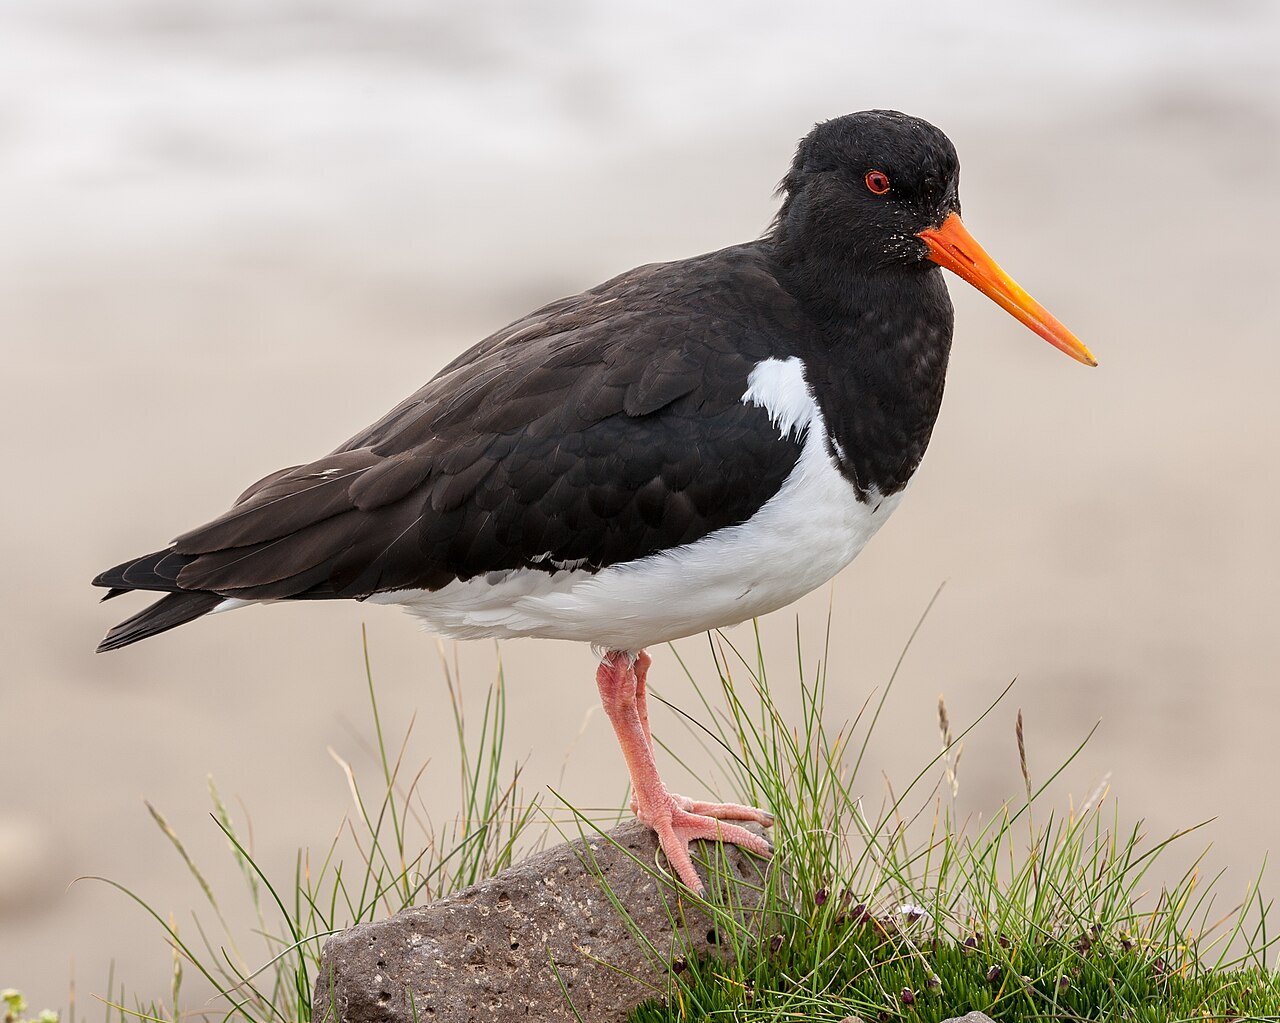
\includegraphics[width=0.8\linewidth, height=10cm, keepaspectratio]{Billeder/Dyr/Fugle/Vadefugle/strandskade.jpg}
\end{minipage}
}%
\end{columns}
\end{frame}
\begin{frame}{%
\begin{minipage}[t]{0.85\textwidth}
Vibe
\end{minipage}%
\hfill
\begin{minipage}[t]{0.1\textwidth}
\raggedleft

\includegraphics[width=0.55cm, height=0.55cm, keepaspectratio]{Billeder/Ikoner/star.png}%
\end{minipage}%
}
\vspace{0.25em}
\begin{columns}[T]
% --- Venstre kolonne: Tekst ---
\column{0.55\textwidth}
\setlength{\parskip}{0.5em}
\small
\RaggedRight\textbf{\textit{Vanellus vanellus}} – karakteristisk med fjertoppen på hvoedet\par

\textbf{Udseende:} \\
\quad –  Metalgrøn ryg, hvid bug, sort bryst og pande. Lang nakketop på hovedet.   

% --- Højre kolonne: Et billede ---
\column{0.40\textwidth}
\centering
\fbox{%
\begin{minipage}{\linewidth}
\centering
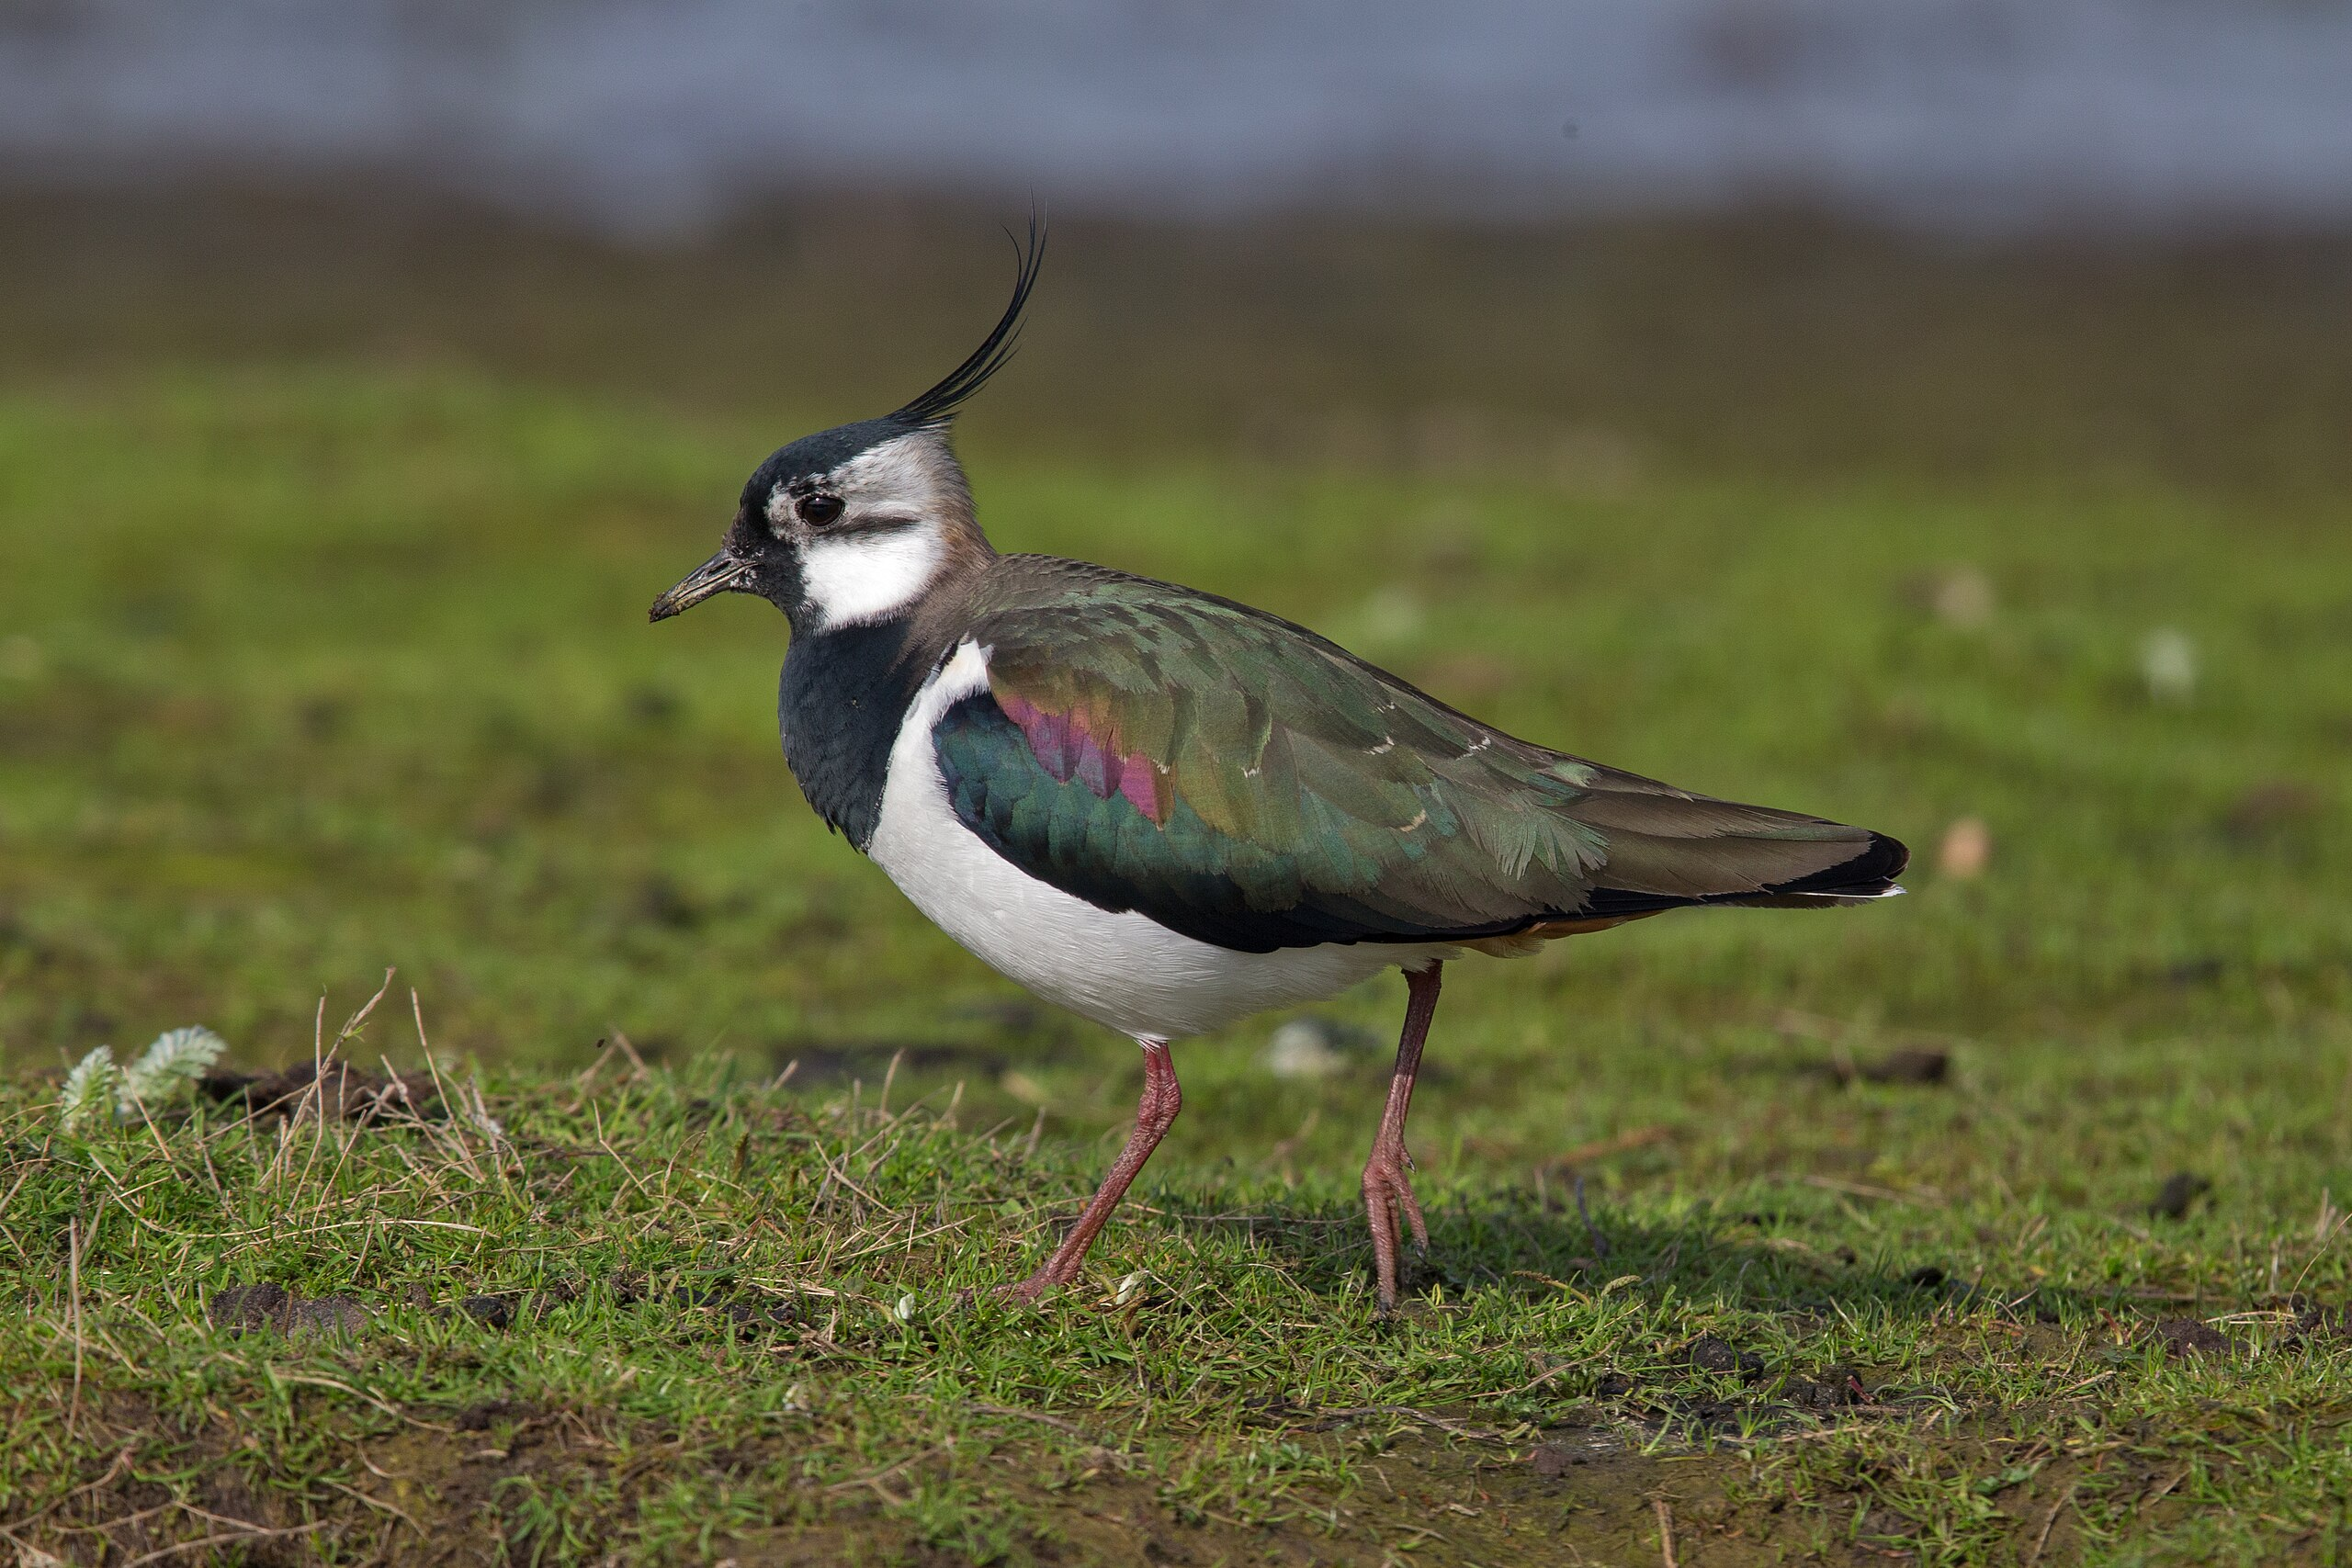
\includegraphics[width=0.8\linewidth, height=10cm, keepaspectratio]{Billeder/Dyr/Fugle/Vadefugle/vibe.jpg}
\end{minipage}
}%
\end{columns}
\end{frame}
\begin{frame}{%
\begin{minipage}[t]{0.85\textwidth}
Hjejle
\end{minipage}%
\hfill
\begin{minipage}[t]{0.1\textwidth}
\raggedleft

\includegraphics[width=0.5cm, height=0.5cm, keepaspectratio]{Billeder/Ikoner/star.png}%
\hspace{0.2em}%

\includegraphics[width=0.5cm, height=0.5cm, keepaspectratio]{Billeder/Ikoner/star.png}
\end{minipage}%
}
\vspace{0.25em}
\begin{columns}[T]
% --- Venstre kolonne: Tekst ---
\column{0.55\textwidth}
\setlength{\parskip}{0.5em}
\small
\RaggedRight\textbf{\textit{Pluvialis apricaria}} – Mellemstor vadefugl som kan forveksles med strandhjejle\par 

\textbf{Udseende:} \\
\quad – Buttet krop, store øjne, rundt hoved og kort næb. Spraglet ryg med sort, grøn og hvide nuancer.  \par

\textbf{Levesteder:} \\
\quad – Marker og enge, primært Vestjylland

\textbf{Føde:} \\
\quad – Primært animals: orme, insekter, snegle  \par

\textbf{Udbredelse:} \\
\quad – Sjælden ynglefugl. Ses primært som trækfugl \par

\textbf{Træk/standfugl} \\
\quad – Trækfugl \par

% --- Højre kolonne: Kun ét billede (Hannen) ---
\column{0.40\textwidth}
\centering
\fbox{%
\begin{minipage}{\linewidth}
\centering
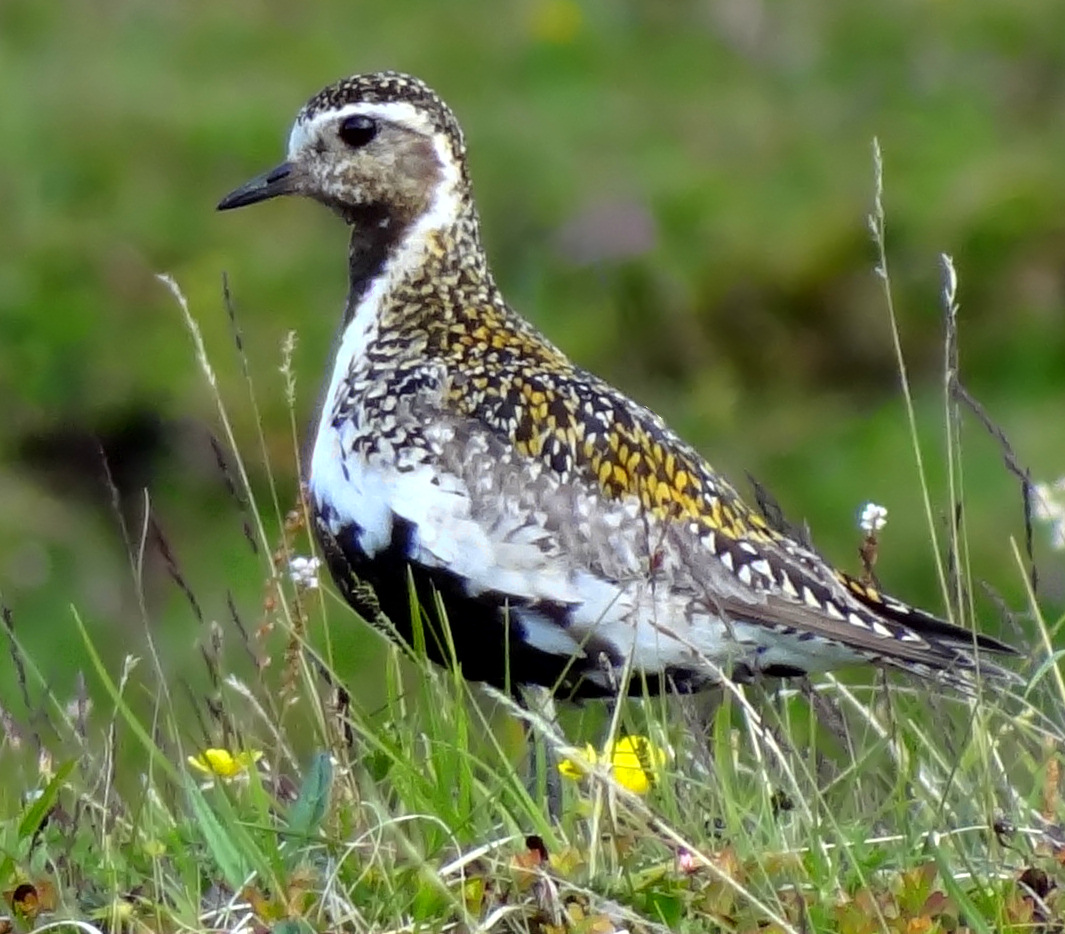
\includegraphics[width=0.8\linewidth, height=6.5cm, keepaspectratio]{Billeder/Dyr/Fugle/Vadefugle/hjejle.jpg}%
\end{minipage}
}%
\end{columns}
\end{frame}
\begin{frame}{%
\begin{minipage}[t]{0.85\textwidth}
Strandhjejle
\end{minipage}%
\hfill
\begin{minipage}[t]{0.1\textwidth}
\raggedleft

\includegraphics[width=0.55cm, height=0.55cm, keepaspectratio]{Billeder/Ikoner/star.png}%
\end{minipage}%
}
\vspace{0.25em}
\begin{columns}[T]
% --- Venstre kolonne: Tekst ---
\column{0.55\textwidth}
\setlength{\parskip}{0.5em}
\small
\RaggedRight\textbf{\textit{Pluvialis squatarola}} – Ligner hjeljlen men har hvid isse\par

\textbf{Udseende:} \\
\quad –  Sort hvid ryg som adskiller den fra hjejlen same den hvide isse  

% --- Højre kolonne: Et billede ---
\column{0.40\textwidth}
\centering
\fbox{%
\begin{minipage}{\linewidth}
\centering
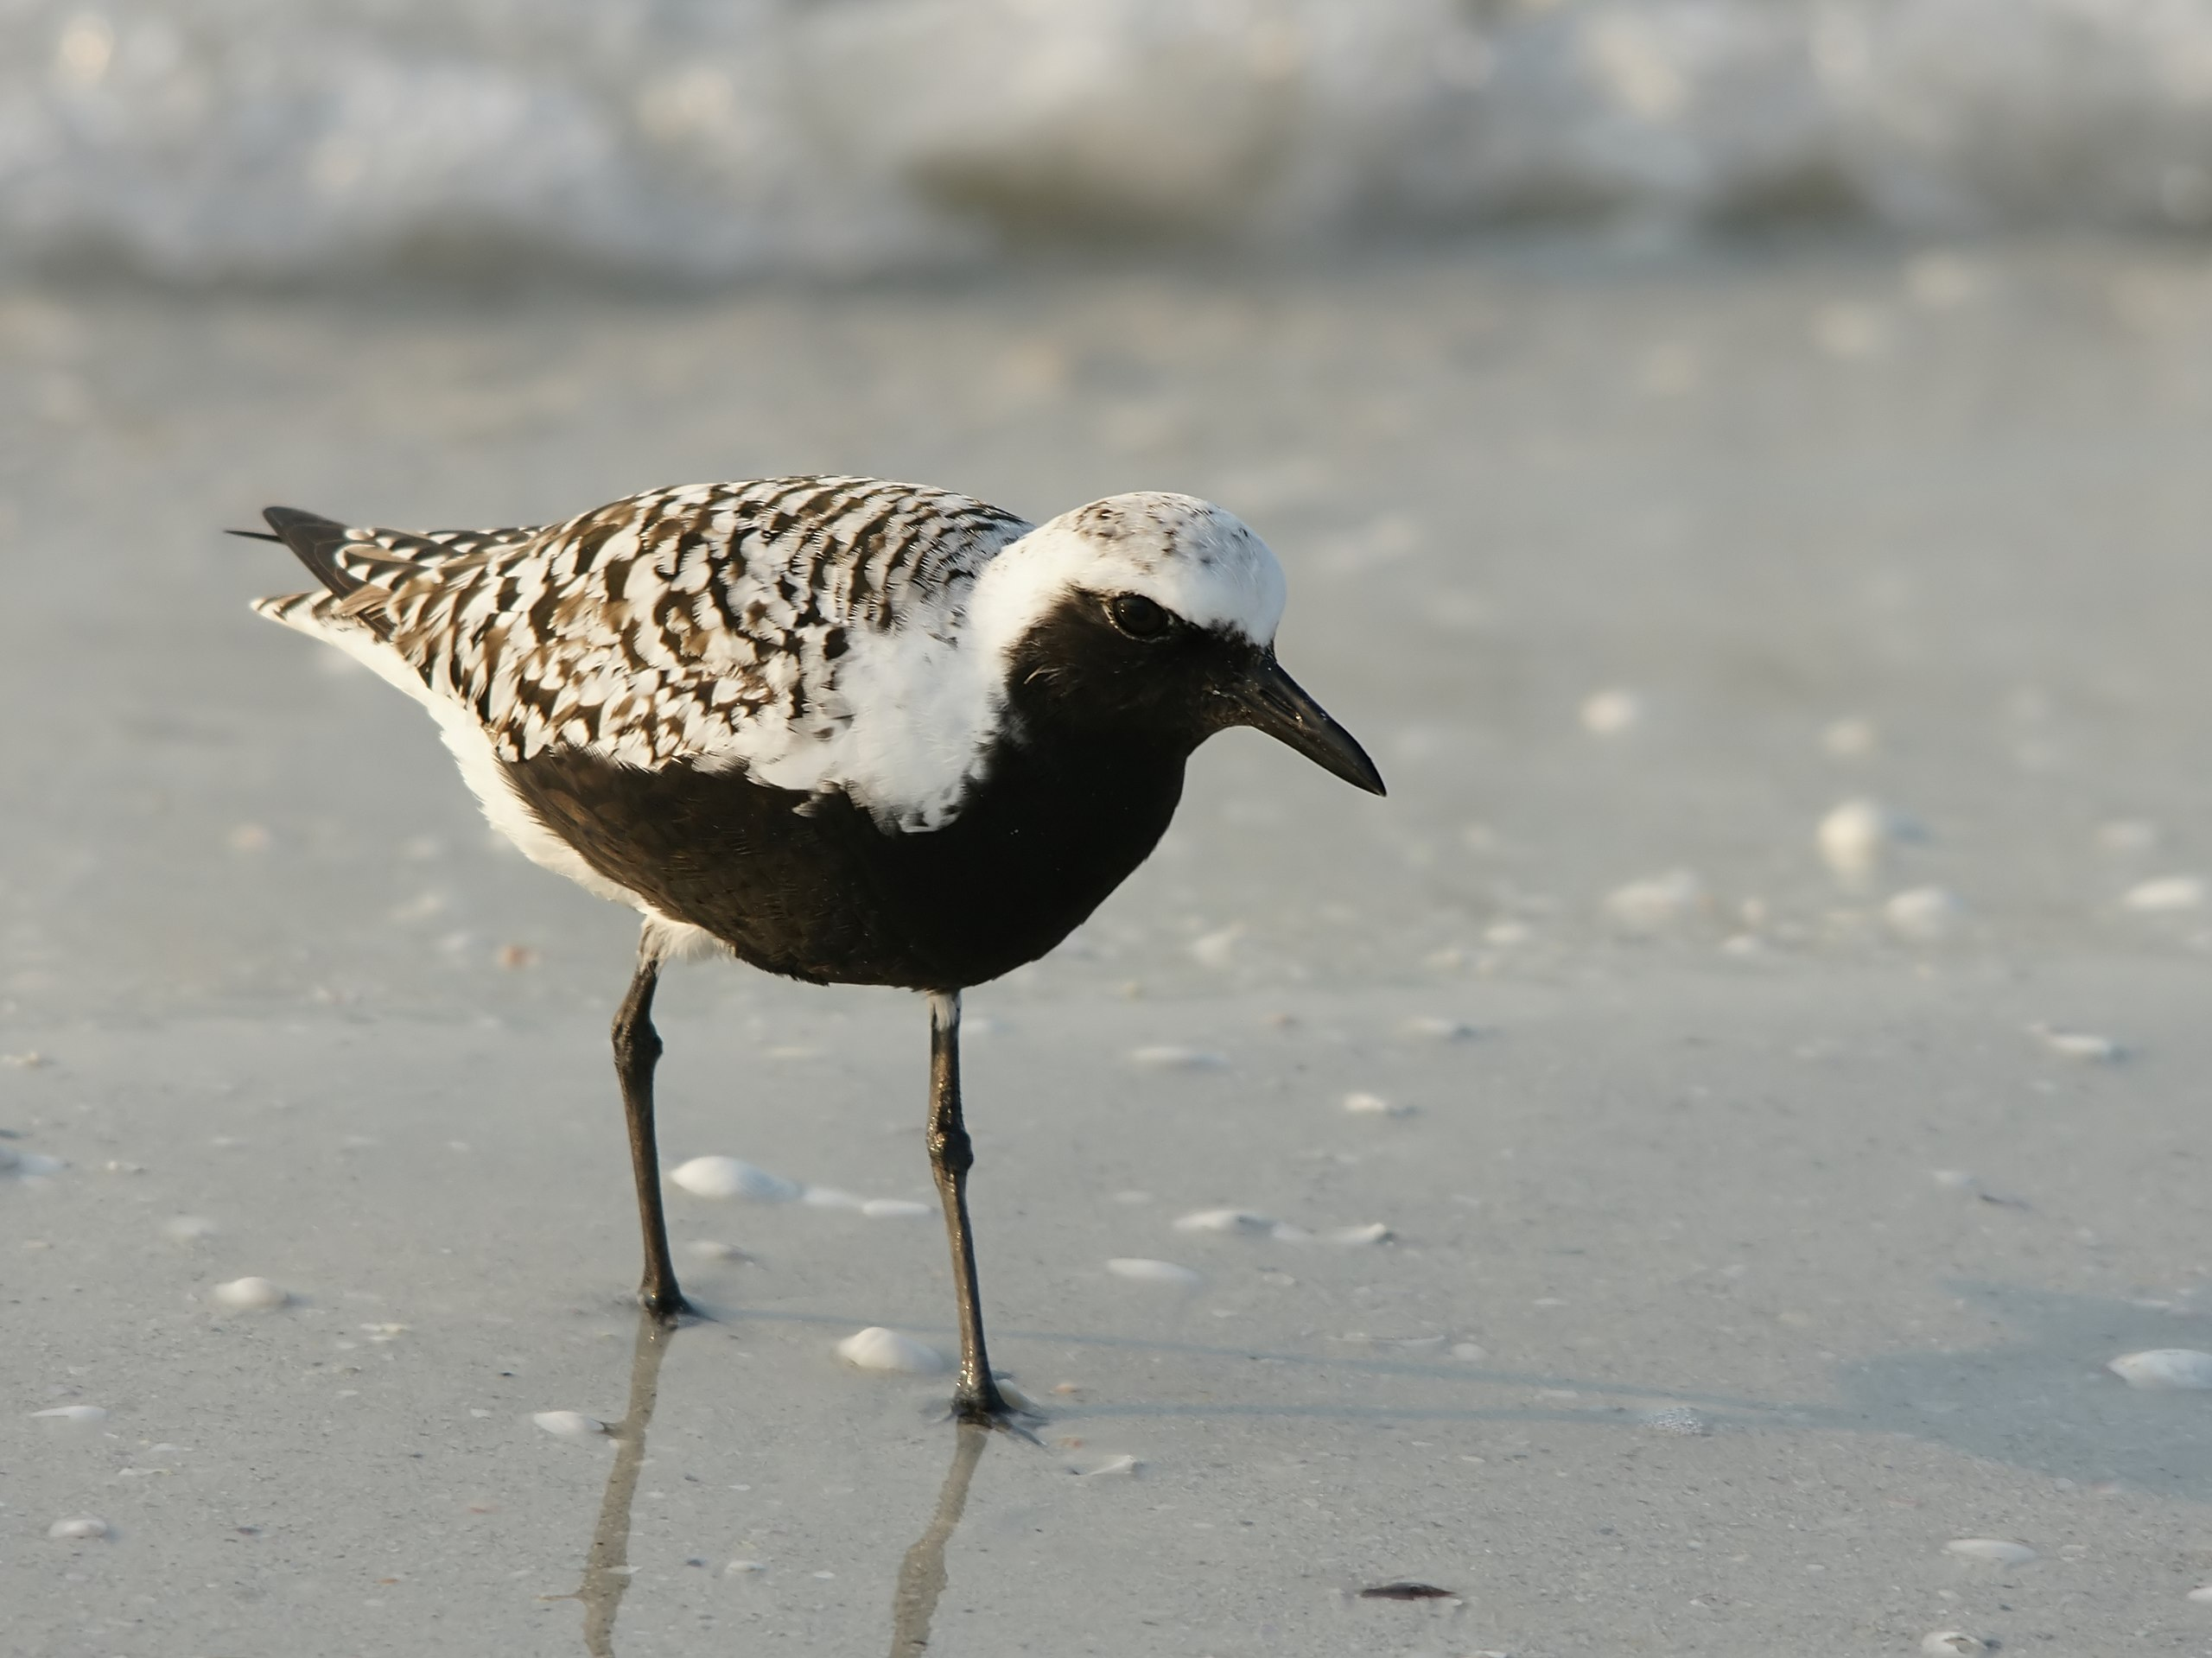
\includegraphics[width=0.8\linewidth, height=10cm, keepaspectratio]{Billeder/Dyr/Fugle/Vadefugle/strandhjejle.jpg}
\end{minipage}
}%
\end{columns}
\end{frame}
\begin{frame}{%
\begin{minipage}[t]{0.85\textwidth}
Stor regnspove
\end{minipage}%
\hfill
\begin{minipage}[t]{0.1\textwidth}
\raggedleft

\includegraphics[width=0.5cm, height=0.5cm, keepaspectratio]{Billeder/Ikoner/star.png}%
\hspace{0.2em}%

\includegraphics[width=0.5cm, height=0.5cm, keepaspectratio]{Billeder/Ikoner/star.png}
\end{minipage}%
}
\vspace{0.25em}
\begin{columns}[T]
% --- Venstre kolonne: Tekst ---
\column{0.55\textwidth}
\setlength{\parskip}{0.5em}
\small
\RaggedRight\textbf{\textit{Numenius arquata}} – Kendes på det lange nedadbøjet næb isse\par 

\textbf{Udseende:} \\
\quad – Kroppen er gråbrun med længdestriber. Næbbet er meget langt og nedadbøjet. Lange ben.  \par

\textbf{Levesteder:} \\
\quad – Kyster, lavvandede søer, enge og heder

\textbf{Føde:} \\
\quad – Børste- og sandorm, snegle, regnorm, insektlarver, krebsydr muslinger og bær \par

\textbf{Udbredelse:} \\
\quad – Primært Jylland \par

\textbf{Træk/standfugl} \\
\quad – Få yngler, alm trækfugl \par

% --- Højre kolonne: Kun ét billede (Hannen) ---
\column{0.40\textwidth}
\centering
\fbox{%
\begin{minipage}{\linewidth}
\centering
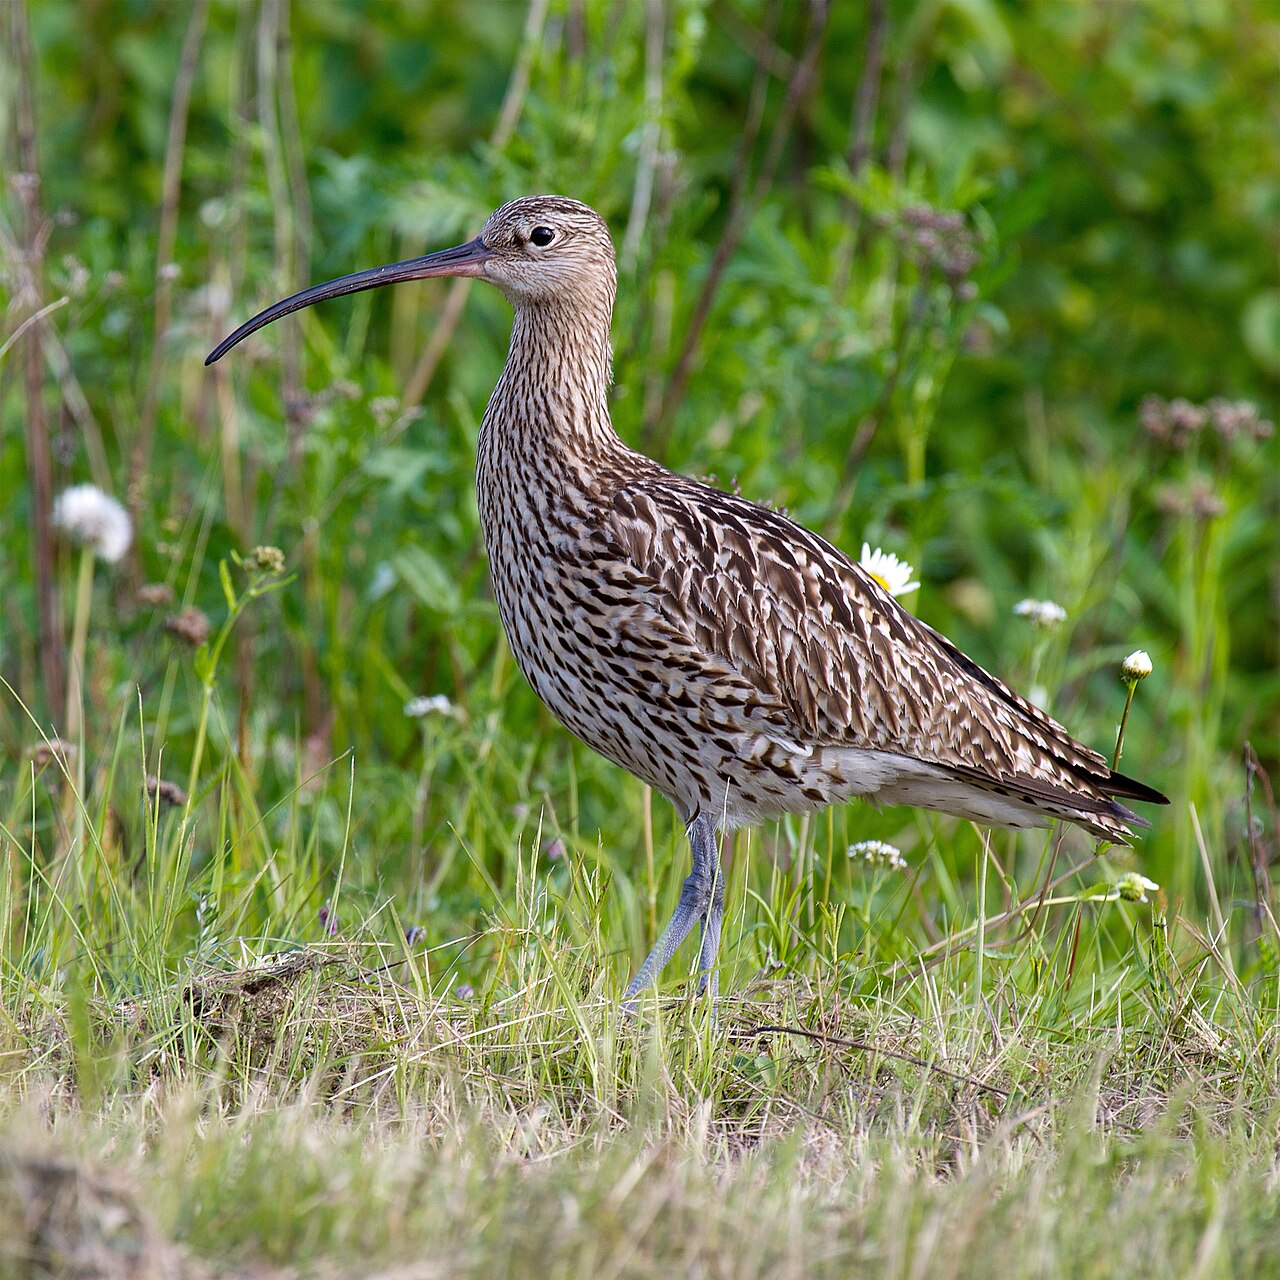
\includegraphics[width=0.8\linewidth, height=6.5cm, keepaspectratio]{Billeder/Dyr/Fugle/Vadefugle/stor_regnspove.jpg}%
\end{minipage}
}%
\end{columns}
\end{frame}
\begin{frame}{%
\begin{minipage}[t]{0.85\textwidth}
Lille regnspove
\end{minipage}%
\hfill
\begin{minipage}[t]{0.1\textwidth}
\raggedleft

\includegraphics[width=0.55cm, height=0.55cm, keepaspectratio]{Billeder/Ikoner/star.png}%
\end{minipage}%
}
\vspace{0.25em}
\begin{columns}[T]
% --- Venstre kolonne: Tekst ---
\column{0.55\textwidth}
\setlength{\parskip}{0.5em}
\small
\RaggedRight\textbf{\textit{Numenius phaeopus}} – også kaldet Småspove, langt nedadbøjet næb \par

\textbf{Udseende:} \\
\quad –  Mørk øjenstribe og tydelige brune issestriber med hvid midterskilning. Langt nedadbøjet næb.  

% --- Højre kolonne: Et billede ---
\column{0.40\textwidth}
\centering
\fbox{%
\begin{minipage}{\linewidth}
\centering
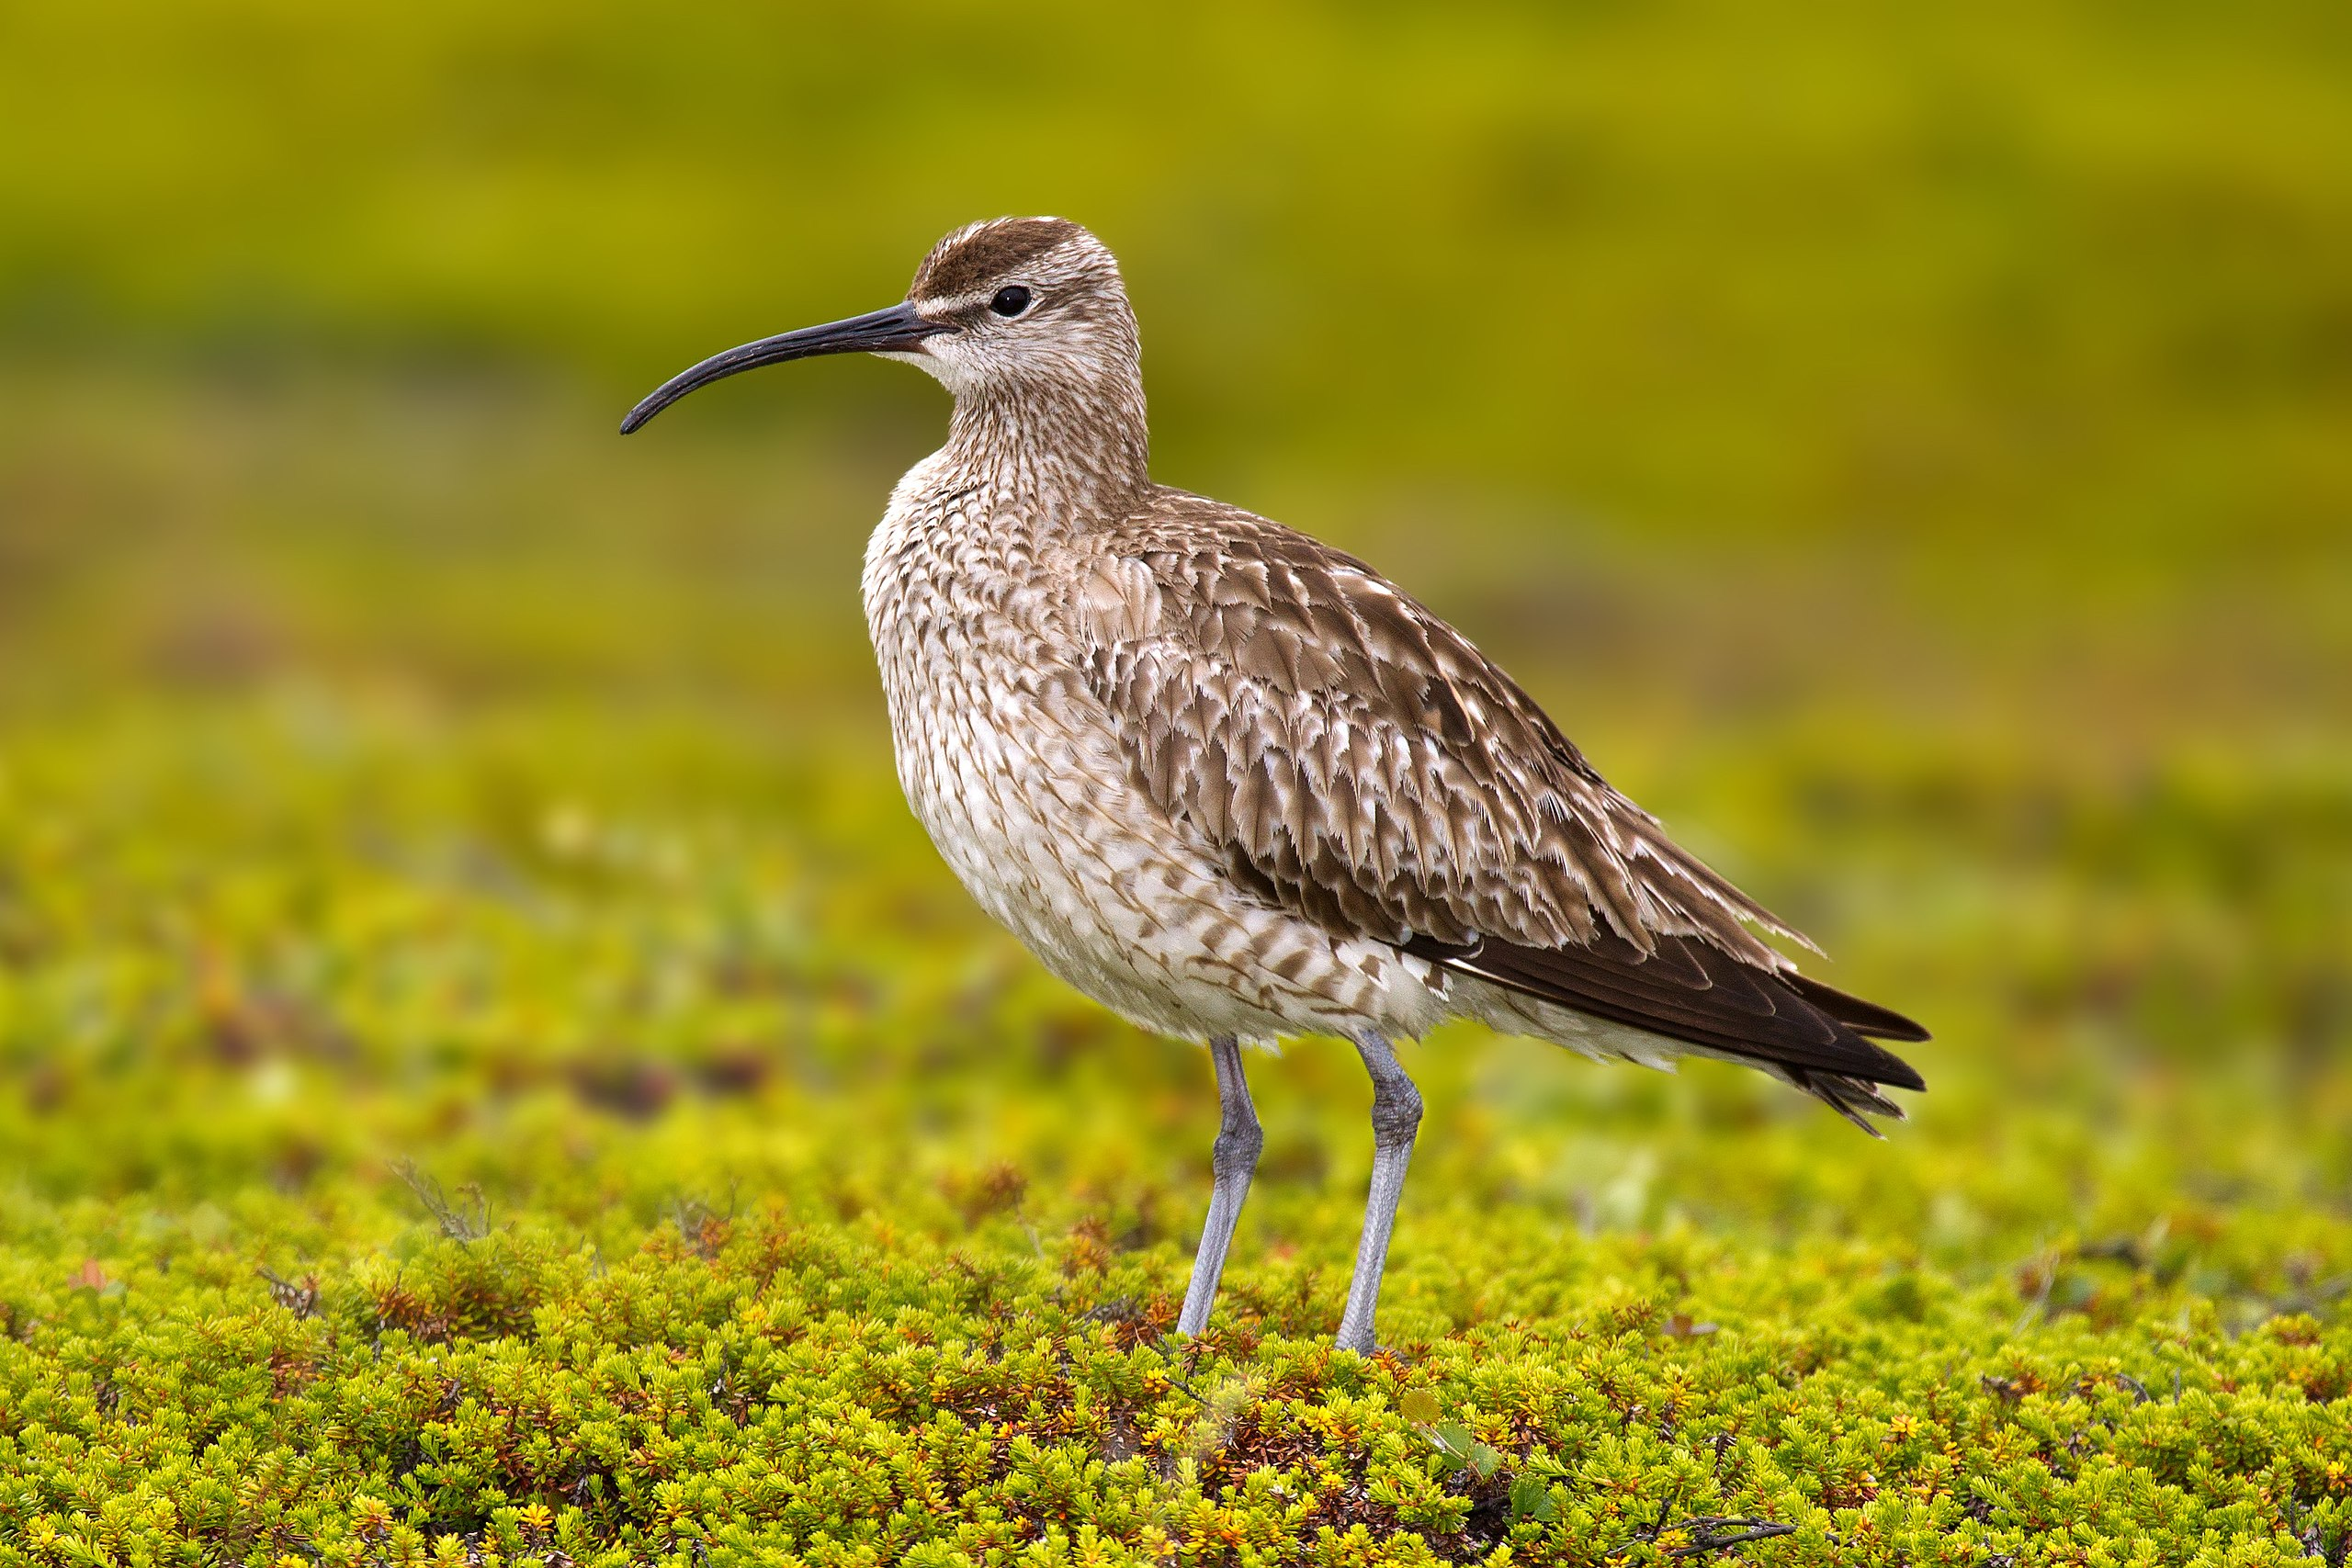
\includegraphics[width=0.8\linewidth, height=10cm, keepaspectratio]{Billeder/Dyr/Fugle/Vadefugle/lille_regnspove.jpg}
\end{minipage}
}%
\end{columns}
\end{frame}



\begin{frame}{%
  \begin{minipage}[t]{0.85\textwidth}
    Lille kobbersneppe
  \end{minipage}%
  \hfill
  \begin{minipage}[t]{0.1\textwidth}
    \raggedleft
    
\includegraphics[width=0.55cm, height=0.55cm, keepaspectratio]{Billeder/Ikoner/star.png}%
  \end{minipage}%
} 
  \vspace{0.25em}
  \begin{columns}[T]
    % --- Venstre kolonne: Tekst ---
    \column{0.55\textwidth}
    \setlength{\parskip}{0.5em}
    \small
    \RaggedRight\textbf{\textit{Limosa lapponica}} – langt næb og lange ben \par

    \textbf{Udseende:} \\
    \quad – Kobberfarvet. Langt let opadbuet næb. Lysere ved næbroden \par

    

    % --- Højre kolonne: To billeder stablet over hinanden ---
    \column{0.40\textwidth}
    \centering
    \fbox{%
      \begin{minipage}{\linewidth}
        \centering
        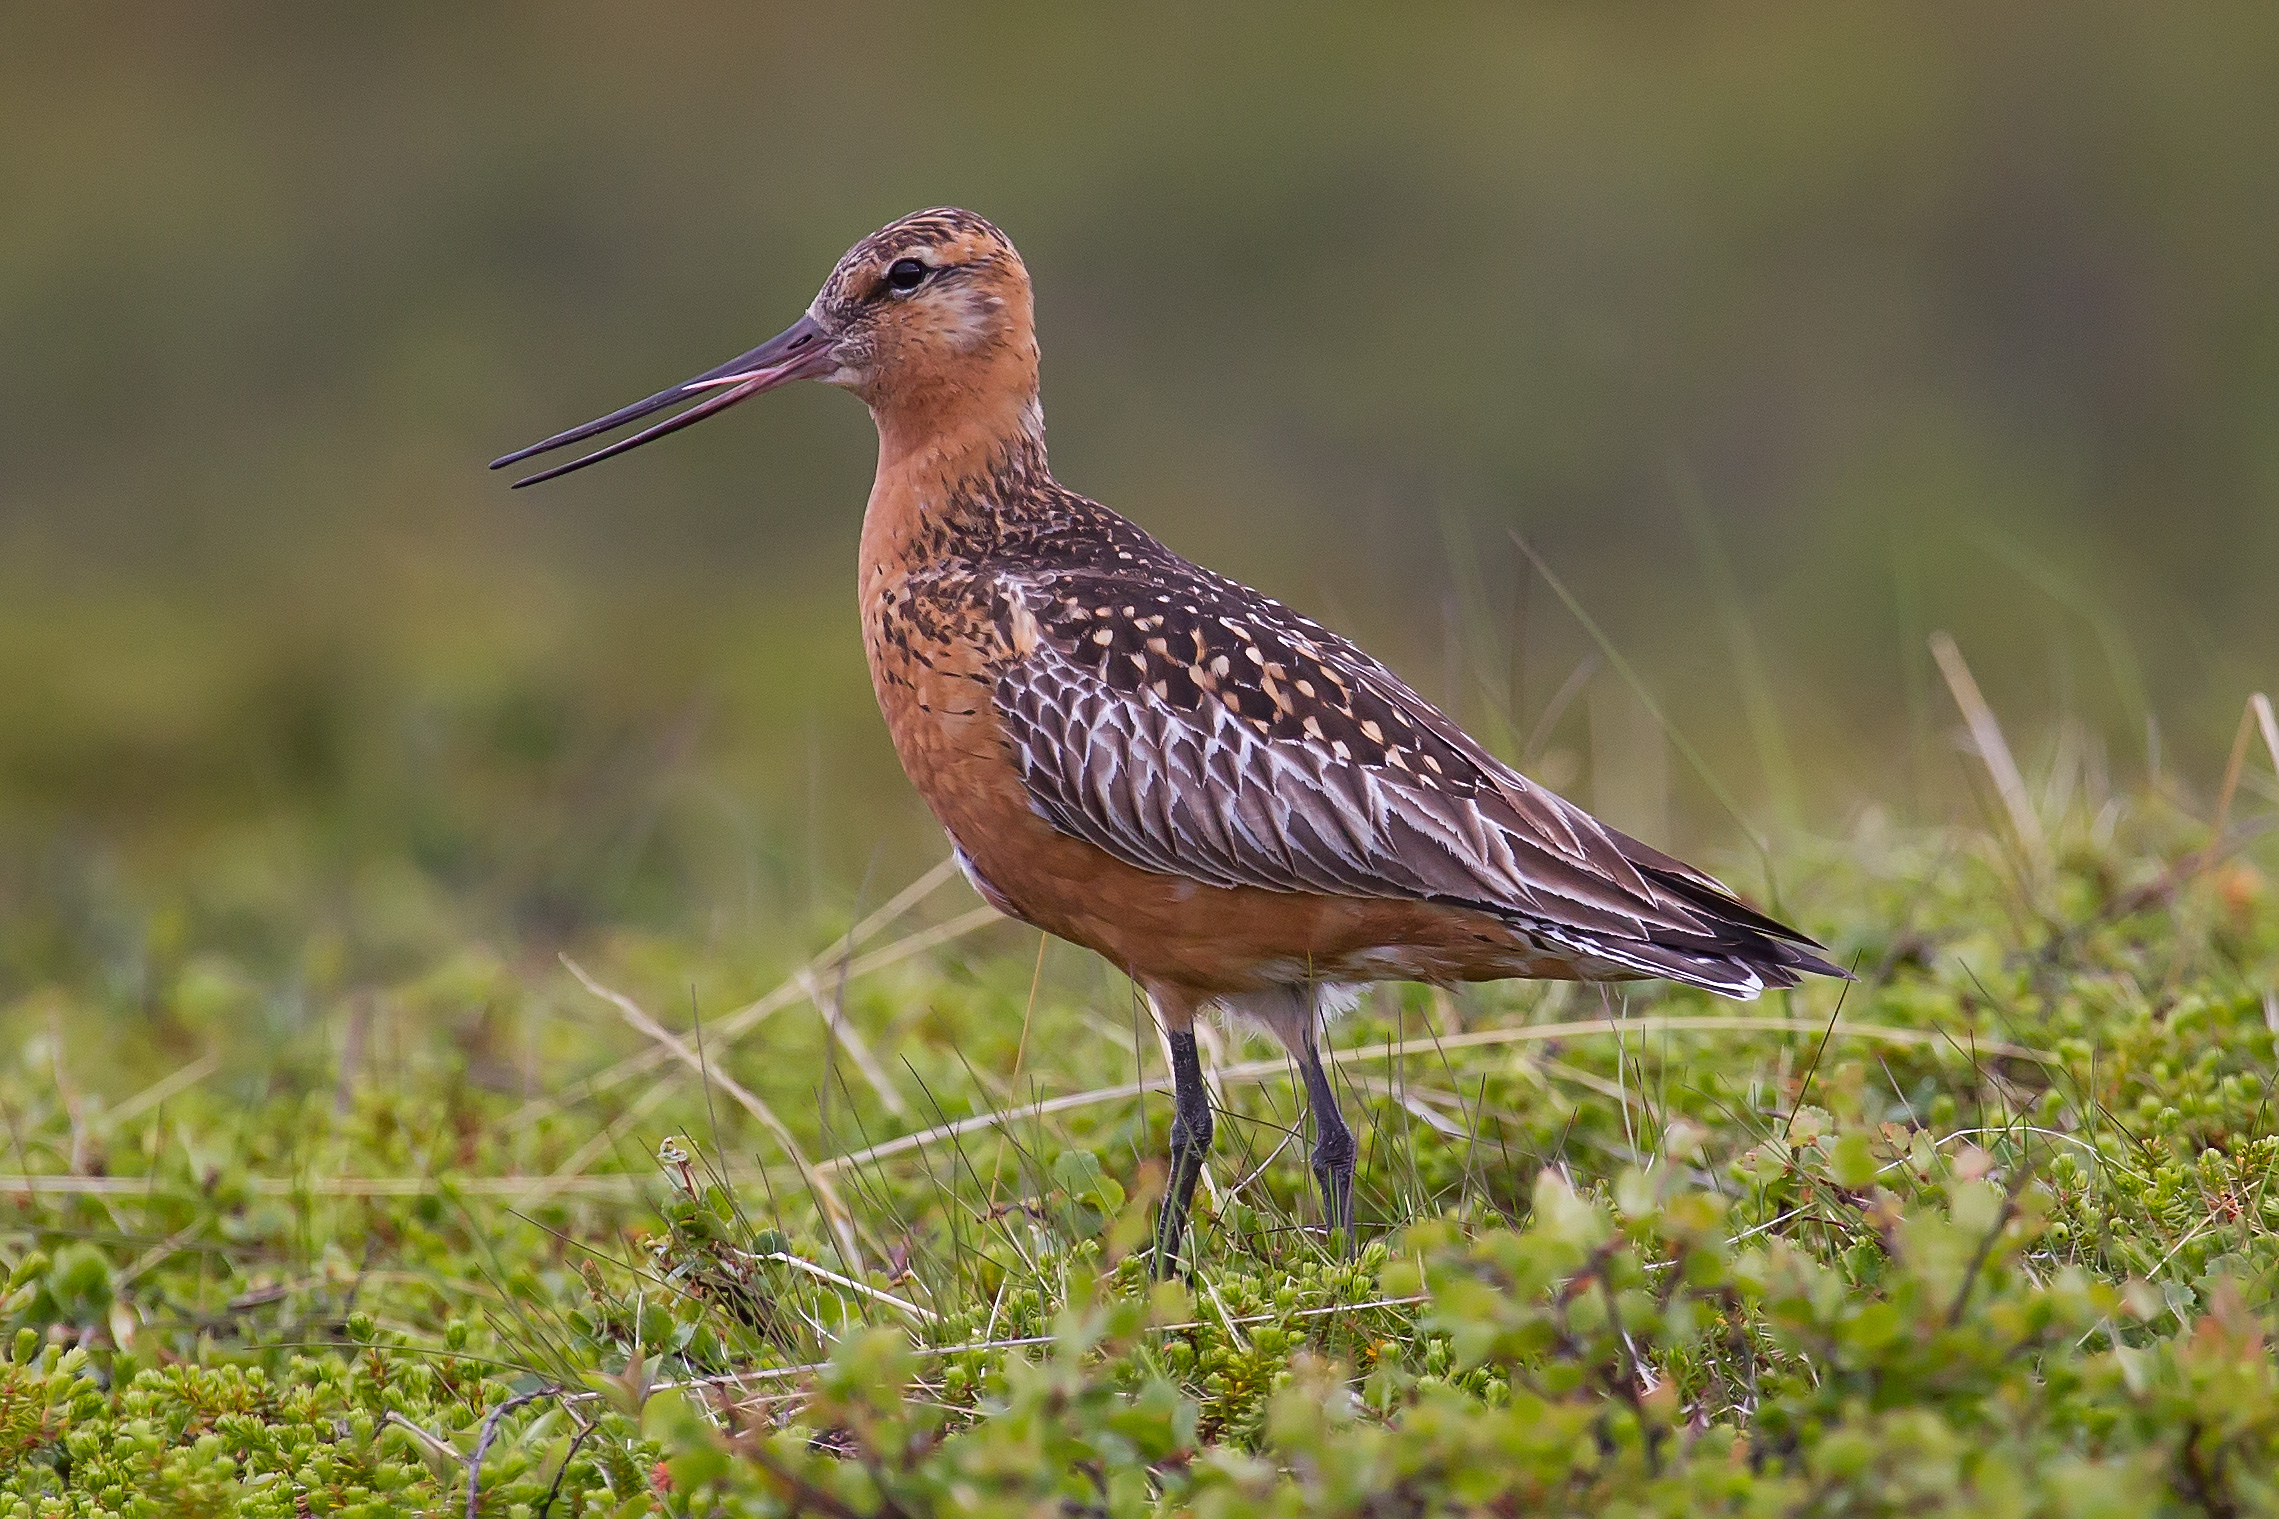
\includegraphics[width=0.8\linewidth, height=3cm, keepaspectratio]{Billeder/Dyr/Fugle/Vadefugle/lille_kobbersneppe_sommer.jpg}\\[0.5em]
        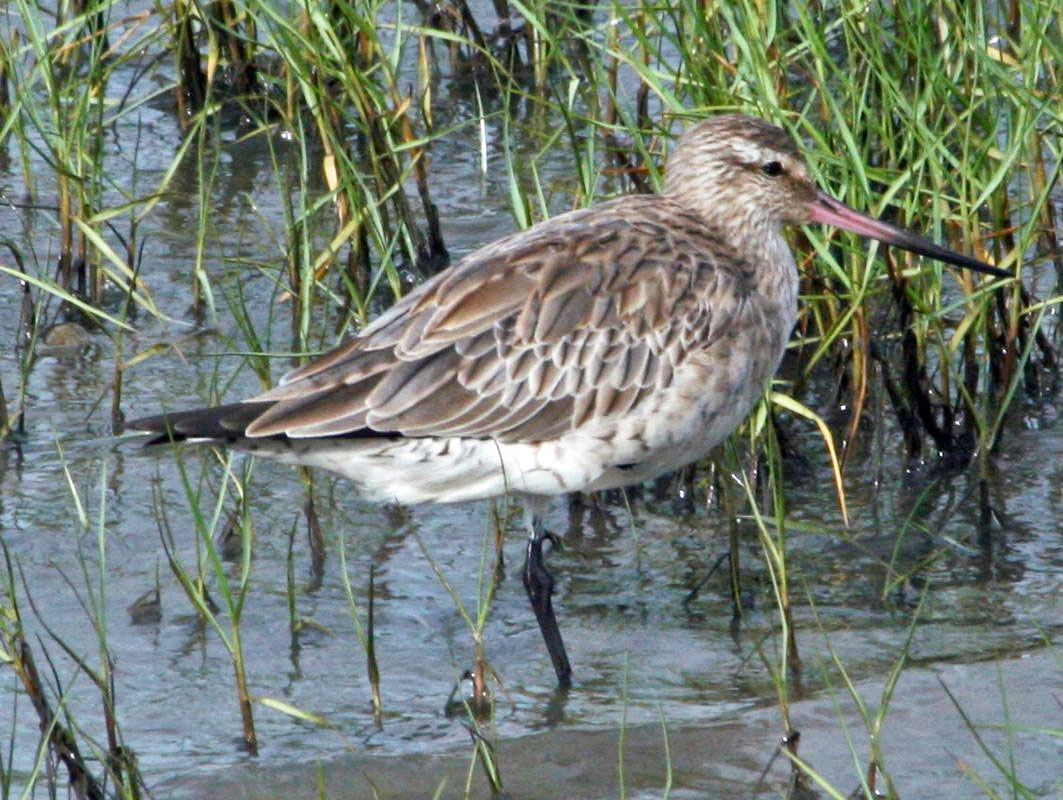
\includegraphics[width=0.8\linewidth, height=3cm, keepaspectratio]{Billeder/Dyr/Fugle/Vadefugle/lille_kobbersneppe_vinter.jpg}%
      \end{minipage}
    }%
    \vspace{0.05em}
    \footnotesize Sommerdragt øverst, vinter nederst
  \end{columns}
\end{frame}
\begin{frame}{%
\begin{minipage}[t]{0.85\textwidth}
Stor kobbersneppe
\end{minipage}%
\hfill
\begin{minipage}[t]{0.1\textwidth}
\raggedleft

\includegraphics[width=0.55cm, height=0.55cm, keepaspectratio]{Billeder/Ikoner/star.png}%
\end{minipage}%
}
\vspace{0.25em}
\begin{columns}[T]
% --- Venstre kolonne: Tekst ---
\column{0.55\textwidth}
\setlength{\parskip}{0.5em}
\small
\RaggedRight\textbf{\textit{Limosa limosa}} – stor slank vadefugl med langt næb\par

\textbf{Udseende:} \\
\quad –  Lange ben og langt svagt opadbuet næb. Næbbet er orangegult med sort spids.   

% --- Højre kolonne: Et billede ---
\column{0.40\textwidth}
\centering
\fbox{%
\begin{minipage}{\linewidth}
\centering
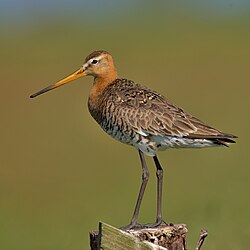
\includegraphics[width=0.8\linewidth, height=10cm, keepaspectratio]{Billeder/Dyr/Fugle/Vadefugle/stor_kobbersneppe.jpg}
\end{minipage}
}%
\end{columns}
\end{frame}
\begin{frame}{%
\begin{minipage}[t]{0.85\textwidth}
Rødben
\end{minipage}%
\hfill
\begin{minipage}[t]{0.1\textwidth}
\raggedleft

\includegraphics[width=0.55cm, height=0.55cm, keepaspectratio]{Billeder/Ikoner/star.png}%
\end{minipage}%
}
\vspace{0.25em}
\begin{columns}[T]
% --- Venstre kolonne: Tekst ---
\column{0.55\textwidth}
\setlength{\parskip}{0.5em}
\small
\RaggedRight\textbf{\textit{Tringa totanus}} – Lys vadefugl med røde ben\par

\textbf{Udseende:} \\
\quad –  Røde ben, rød næb med sort spids.  

% --- Højre kolonne: Et billede ---
\column{0.40\textwidth}
\centering
\fbox{%
\begin{minipage}{\linewidth}
\centering
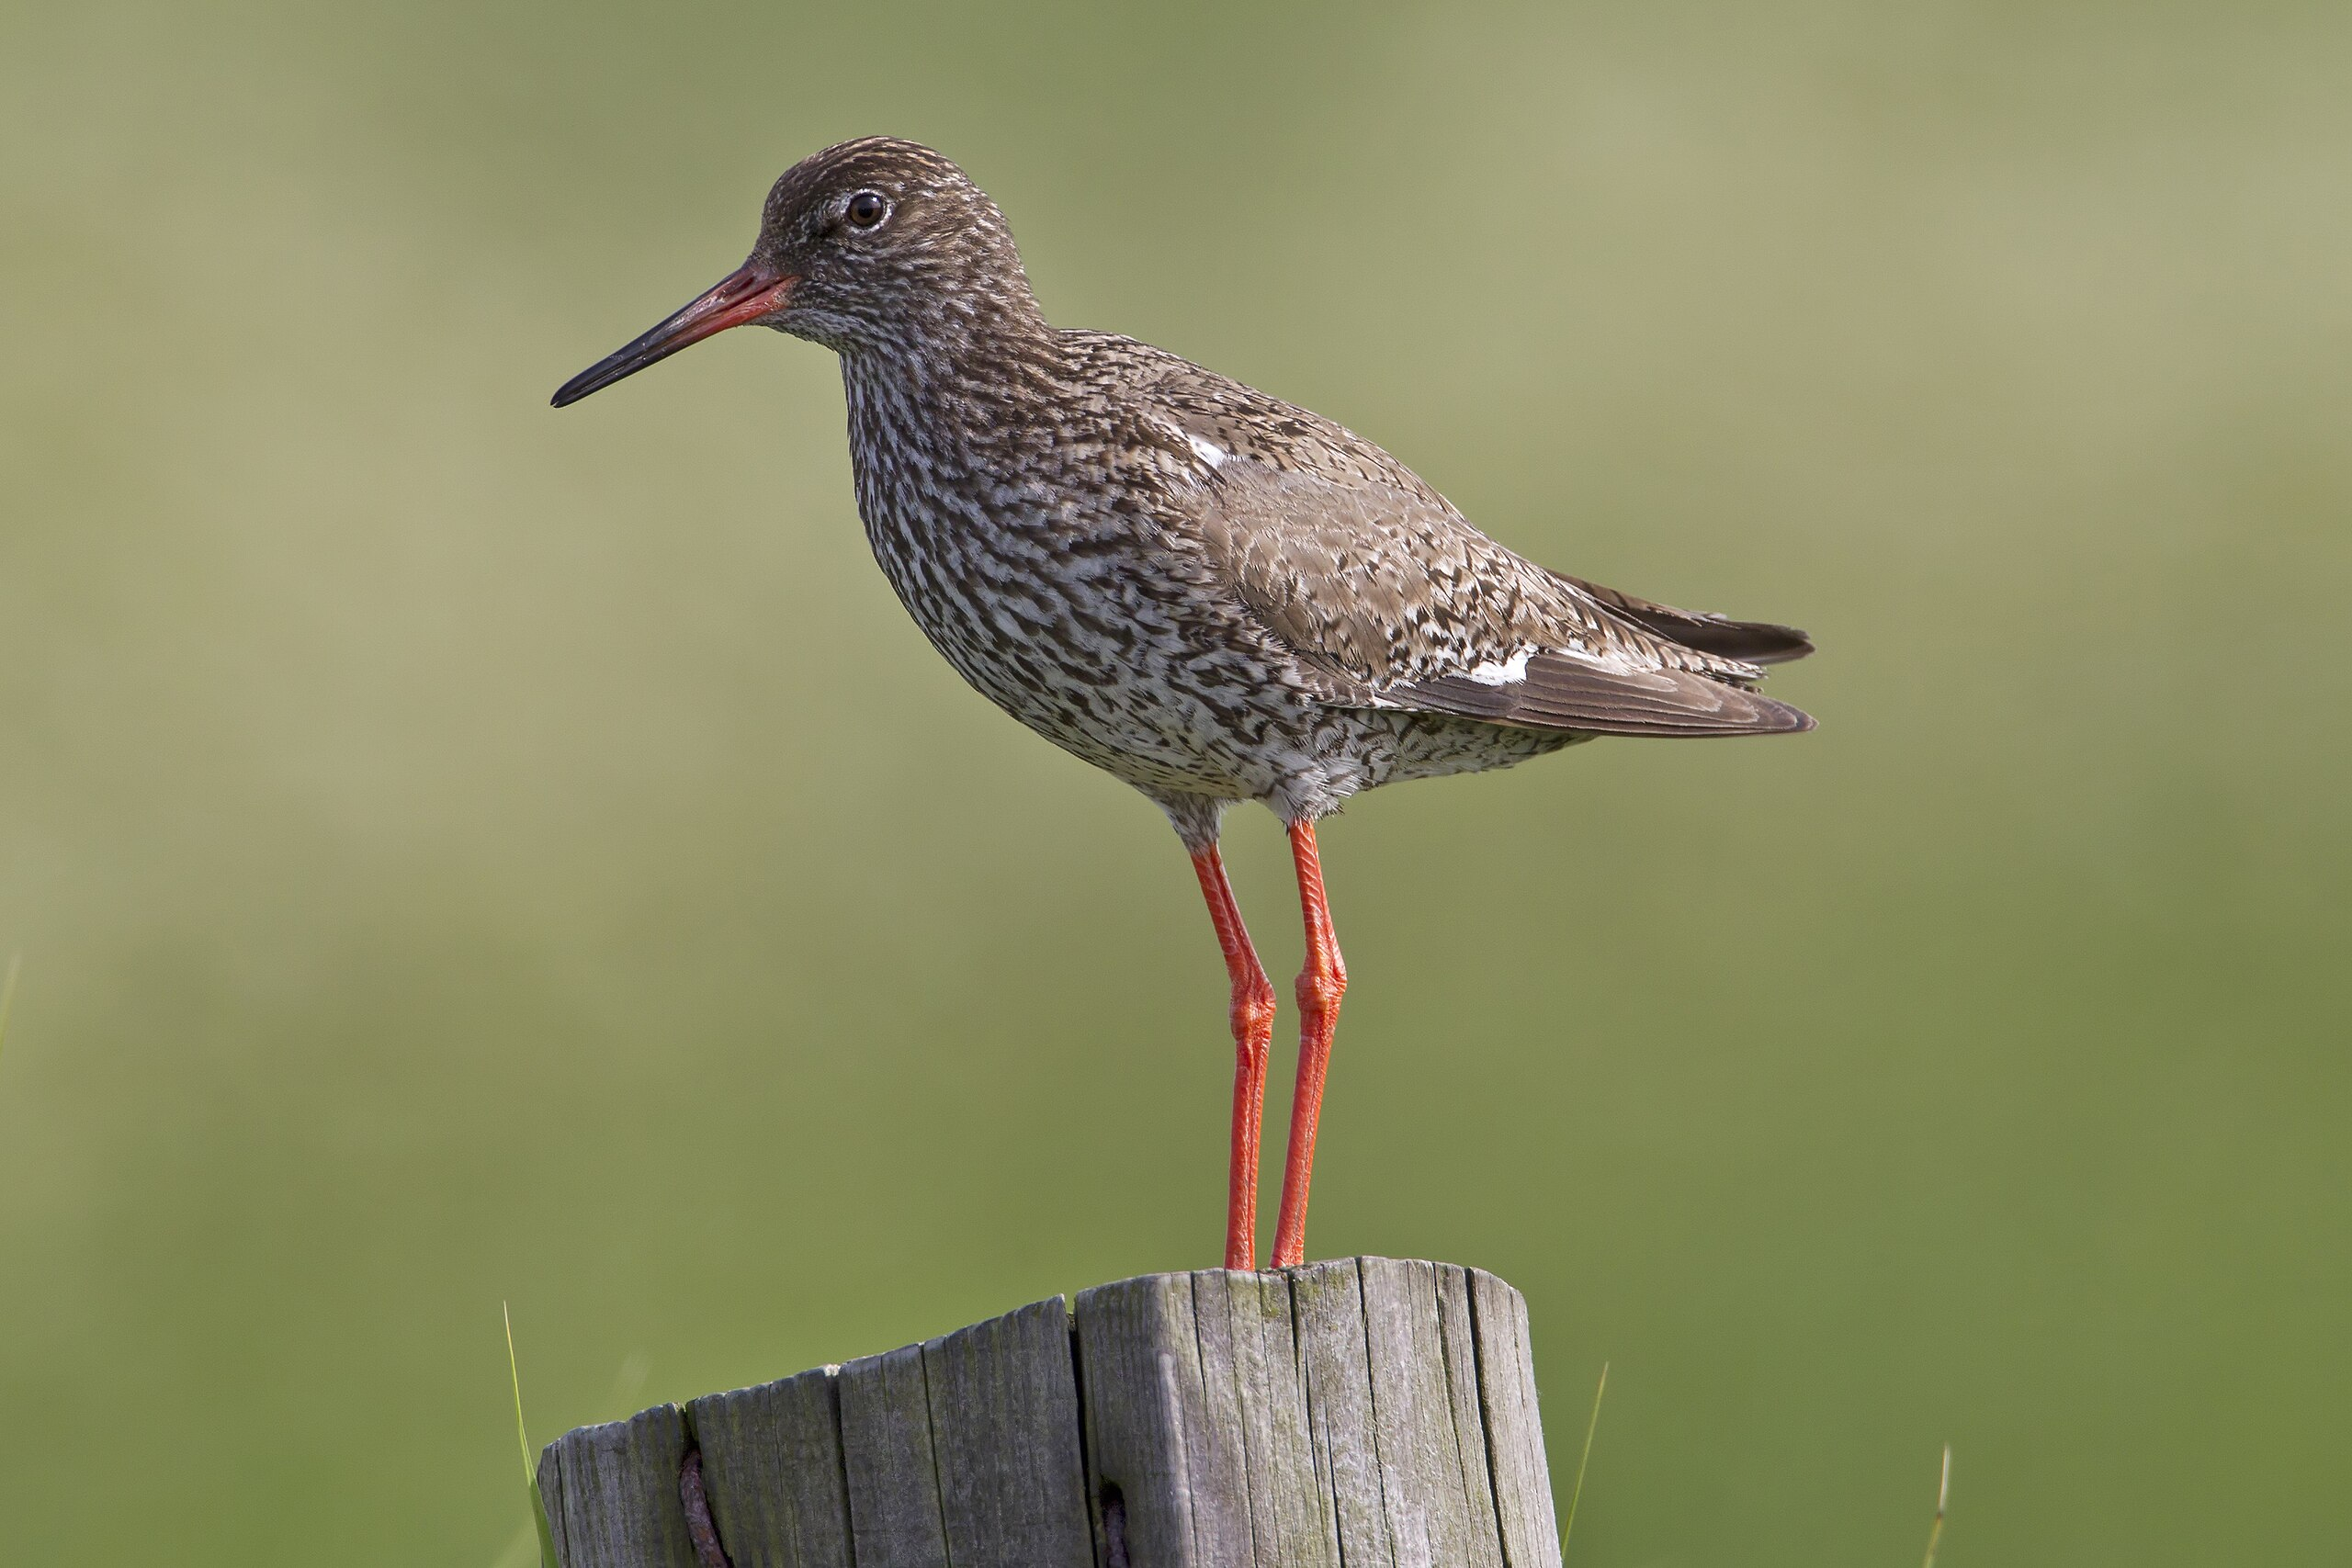
\includegraphics[width=0.8\linewidth, height=10cm, keepaspectratio]{Billeder/Dyr/Fugle/Vadefugle/rødben.jpg}
\end{minipage}
}%
\end{columns}
\end{frame}



\begin{frame}{%
  \begin{minipage}[t]{0.85\textwidth}
    Sortklire
  \end{minipage}%
  \hfill
  \begin{minipage}[t]{0.1\textwidth}
    \raggedleft
    
\includegraphics[width=0.55cm, height=0.55cm, keepaspectratio]{Billeder/Ikoner/star.png}%
  \end{minipage}%
} 
  \vspace{0.25em}
  \begin{columns}[T]
    % --- Venstre kolonne: Tekst ---
    \column{0.55\textwidth}
    \setlength{\parskip}{0.5em}
    \small
    \RaggedRight\textbf{\textit{Tringa erythropus}} – Ligner Rødben men har længere og tyndere næb \par

    \textbf{Udseende:} \\
    \quad – Sort fjerdragt med sorte/mørkerøde ben. Næbbet er lige med svagt dryppende spids. Prikker på oversiden af fjerdragten \par

    

    % --- Højre kolonne: To billeder stablet over hinanden ---
    \column{0.40\textwidth}
    \centering
    \fbox{%
      \begin{minipage}{\linewidth}
        \centering
        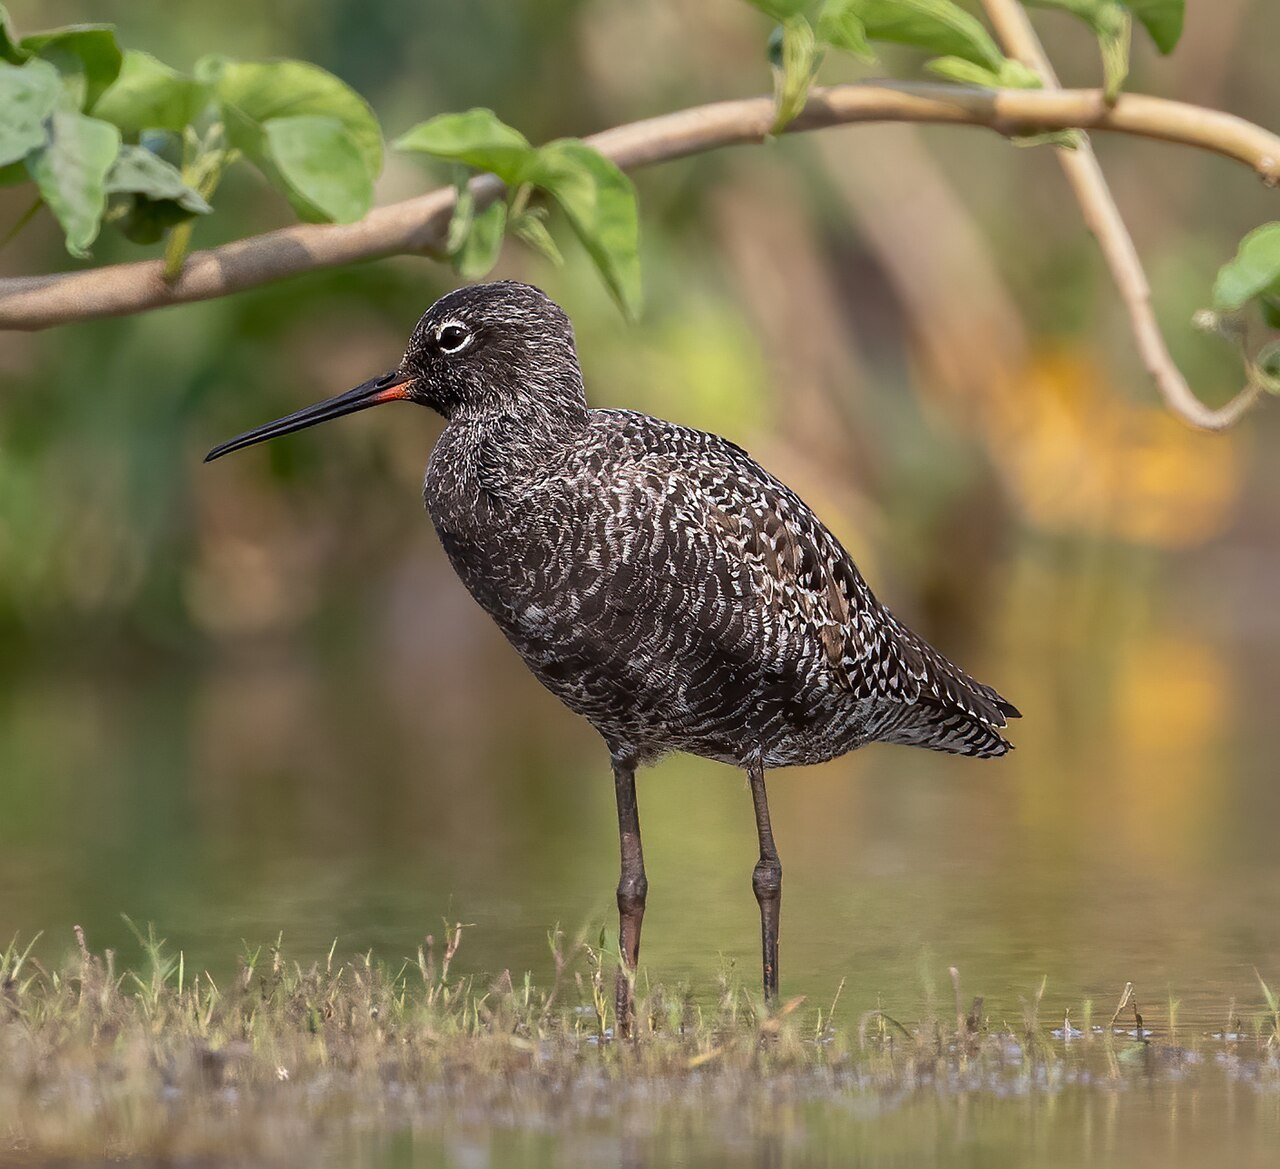
\includegraphics[width=0.8\linewidth, height=3cm, keepaspectratio]{Billeder/Dyr/Fugle/Vadefugle/sortklire_yngledragt.jpg}\\[0.5em]
        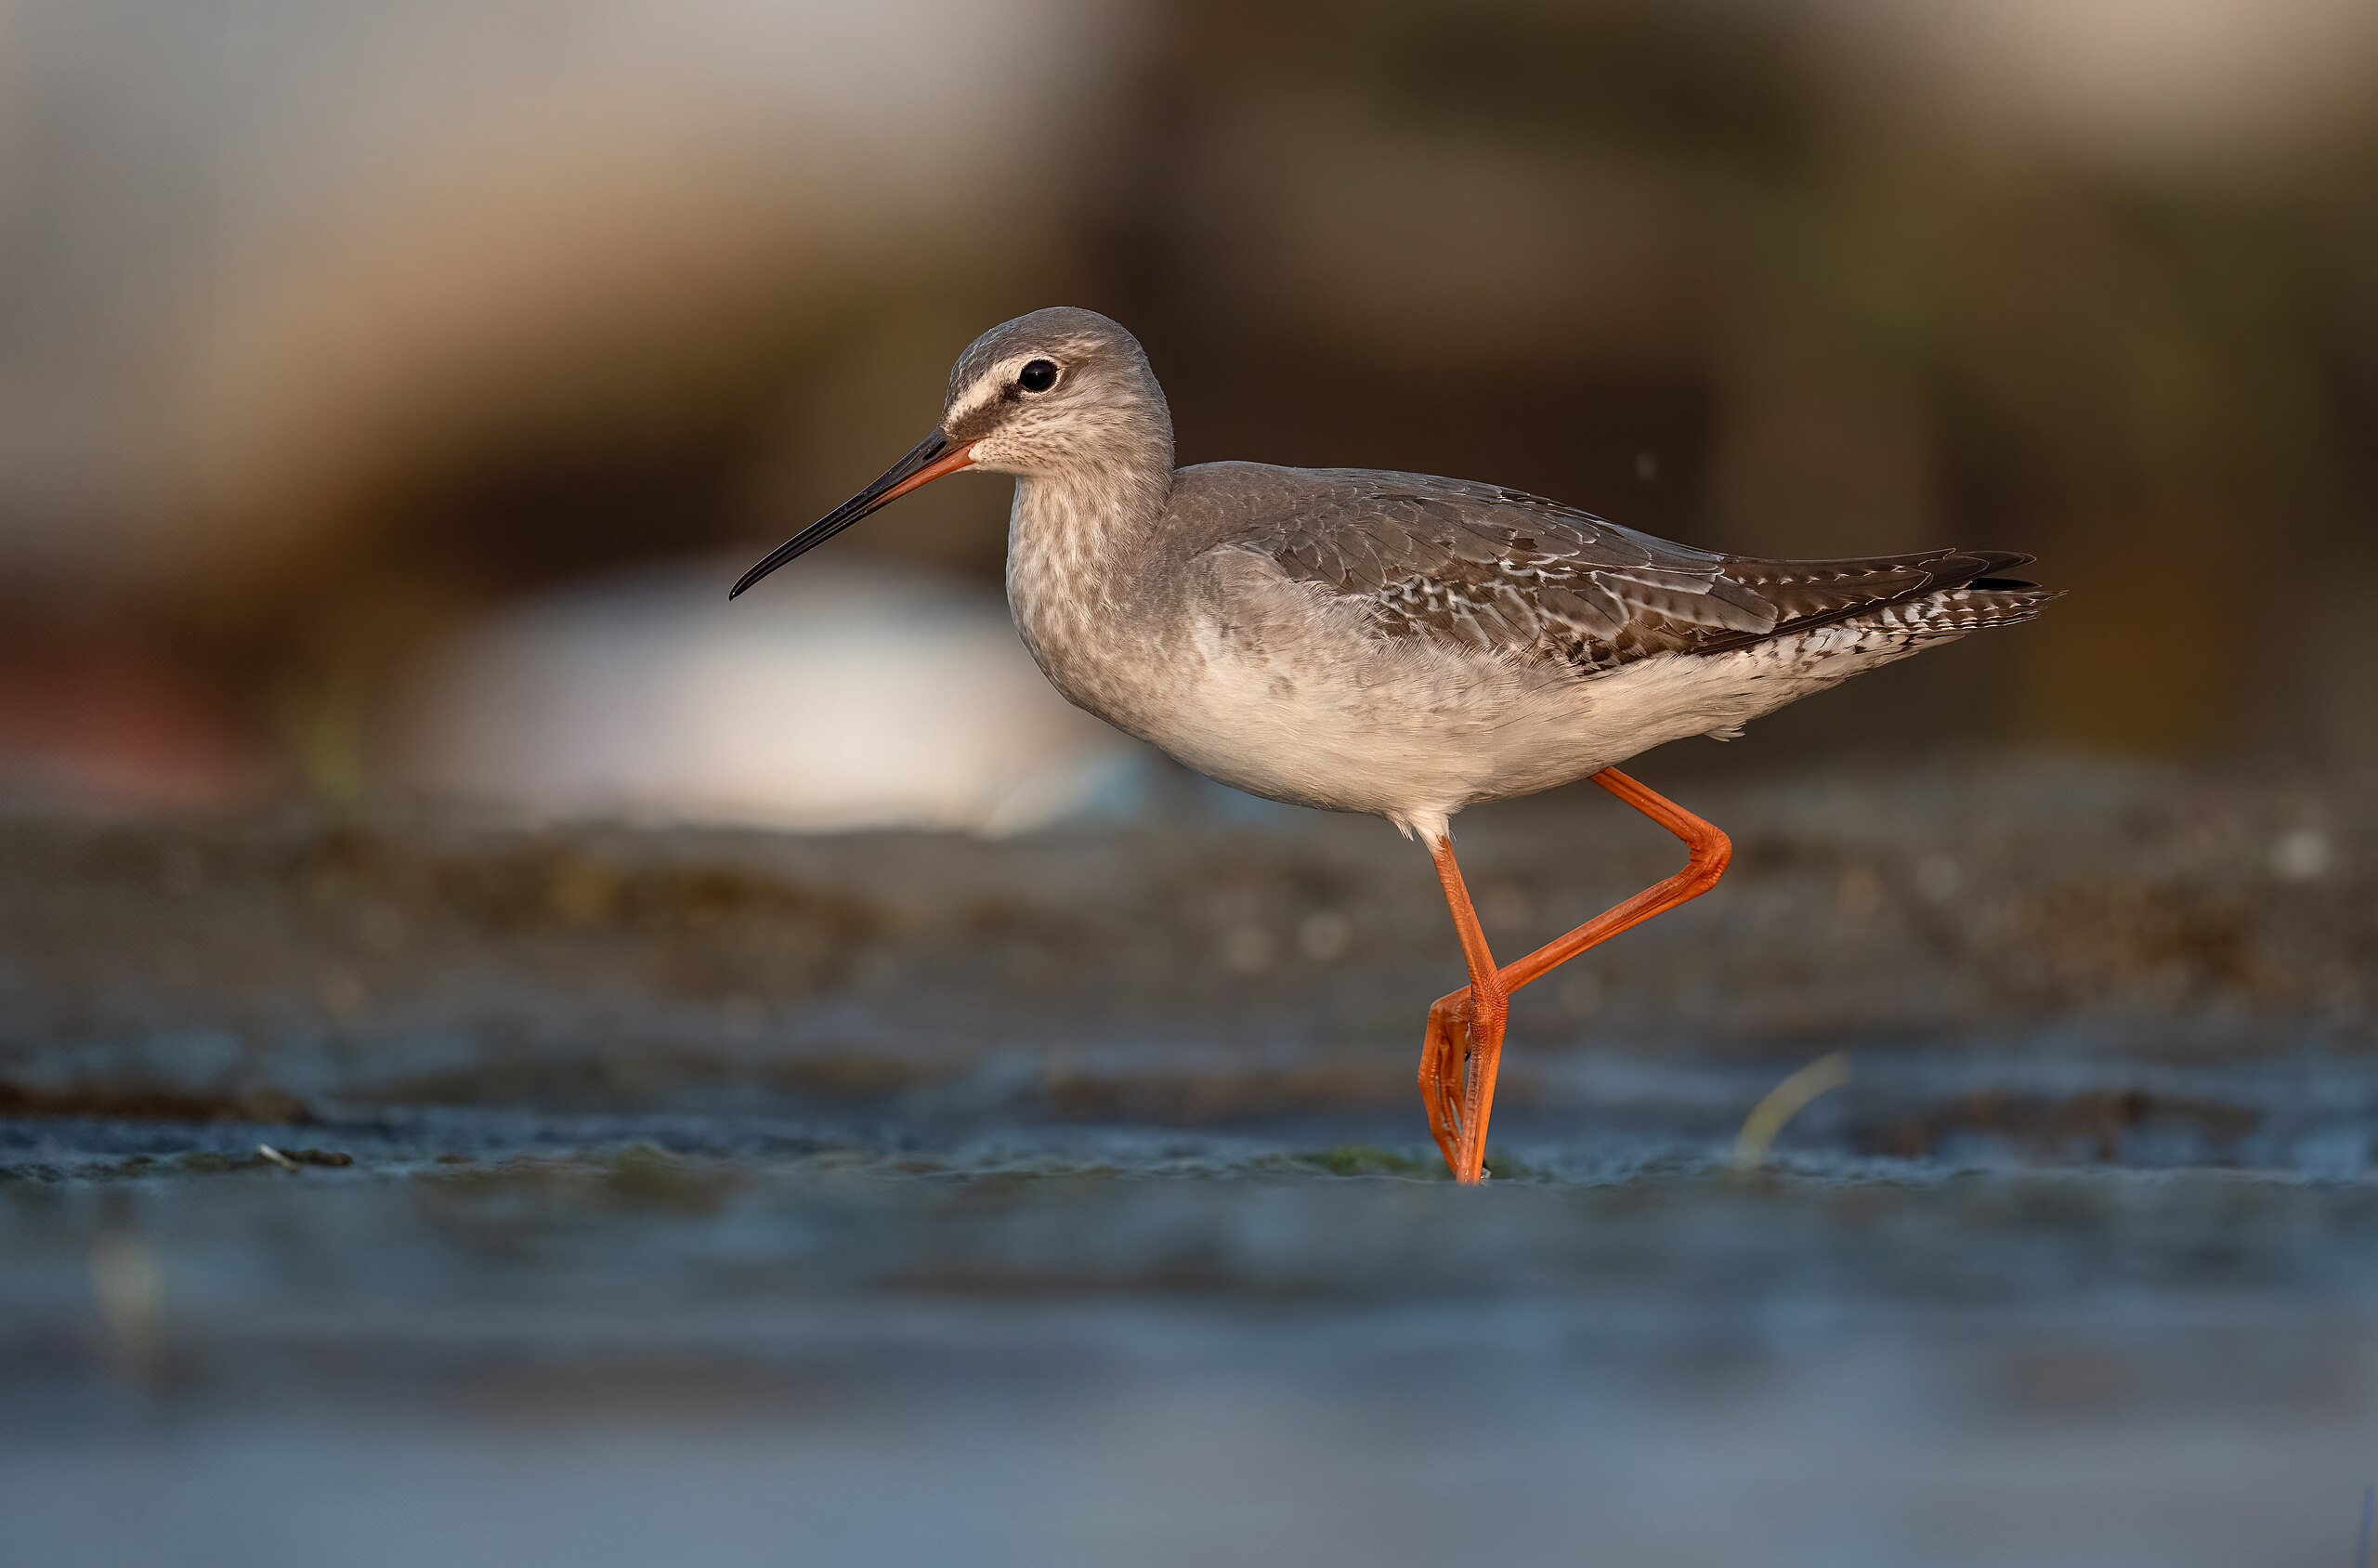
\includegraphics[width=0.8\linewidth, height=3cm, keepaspectratio]{Billeder/Dyr/Fugle/Vadefugle/sortklire_ungfugl.jpg}%
      \end{minipage}
    }%
    \vspace{0.05em}
    \footnotesize Sommer øverst, vinter nederst
  \end{columns}
\end{frame}



\begin{frame}{%
  \begin{minipage}[t]{0.85\textwidth}
    Hvidklire
  \end{minipage}%
  \hfill
  \begin{minipage}[t]{0.1\textwidth}
    \raggedleft
    
\includegraphics[width=0.55cm, height=0.55cm, keepaspectratio]{Billeder/Ikoner/star.png}%
  \end{minipage}%
} 
  \vspace{0.25em}
  \begin{columns}[T]
    % --- Venstre kolonne: Tekst ---
    \column{0.55\textwidth}
    \setlength{\parskip}{0.5em}
    \small
    \RaggedRight\textbf{\textit{Tringa nebularia}} – Trækfugl i Danmark som før hed grønben \par

    \textbf{Udseende:} \\
    \quad – Grønne ben og langt grågrønt let opadbuet næb

    

    % --- Højre kolonne: To billeder stablet over hinanden ---
    \column{0.40\textwidth}
    \centering
    \fbox{%
      \begin{minipage}{\linewidth}
        \centering
        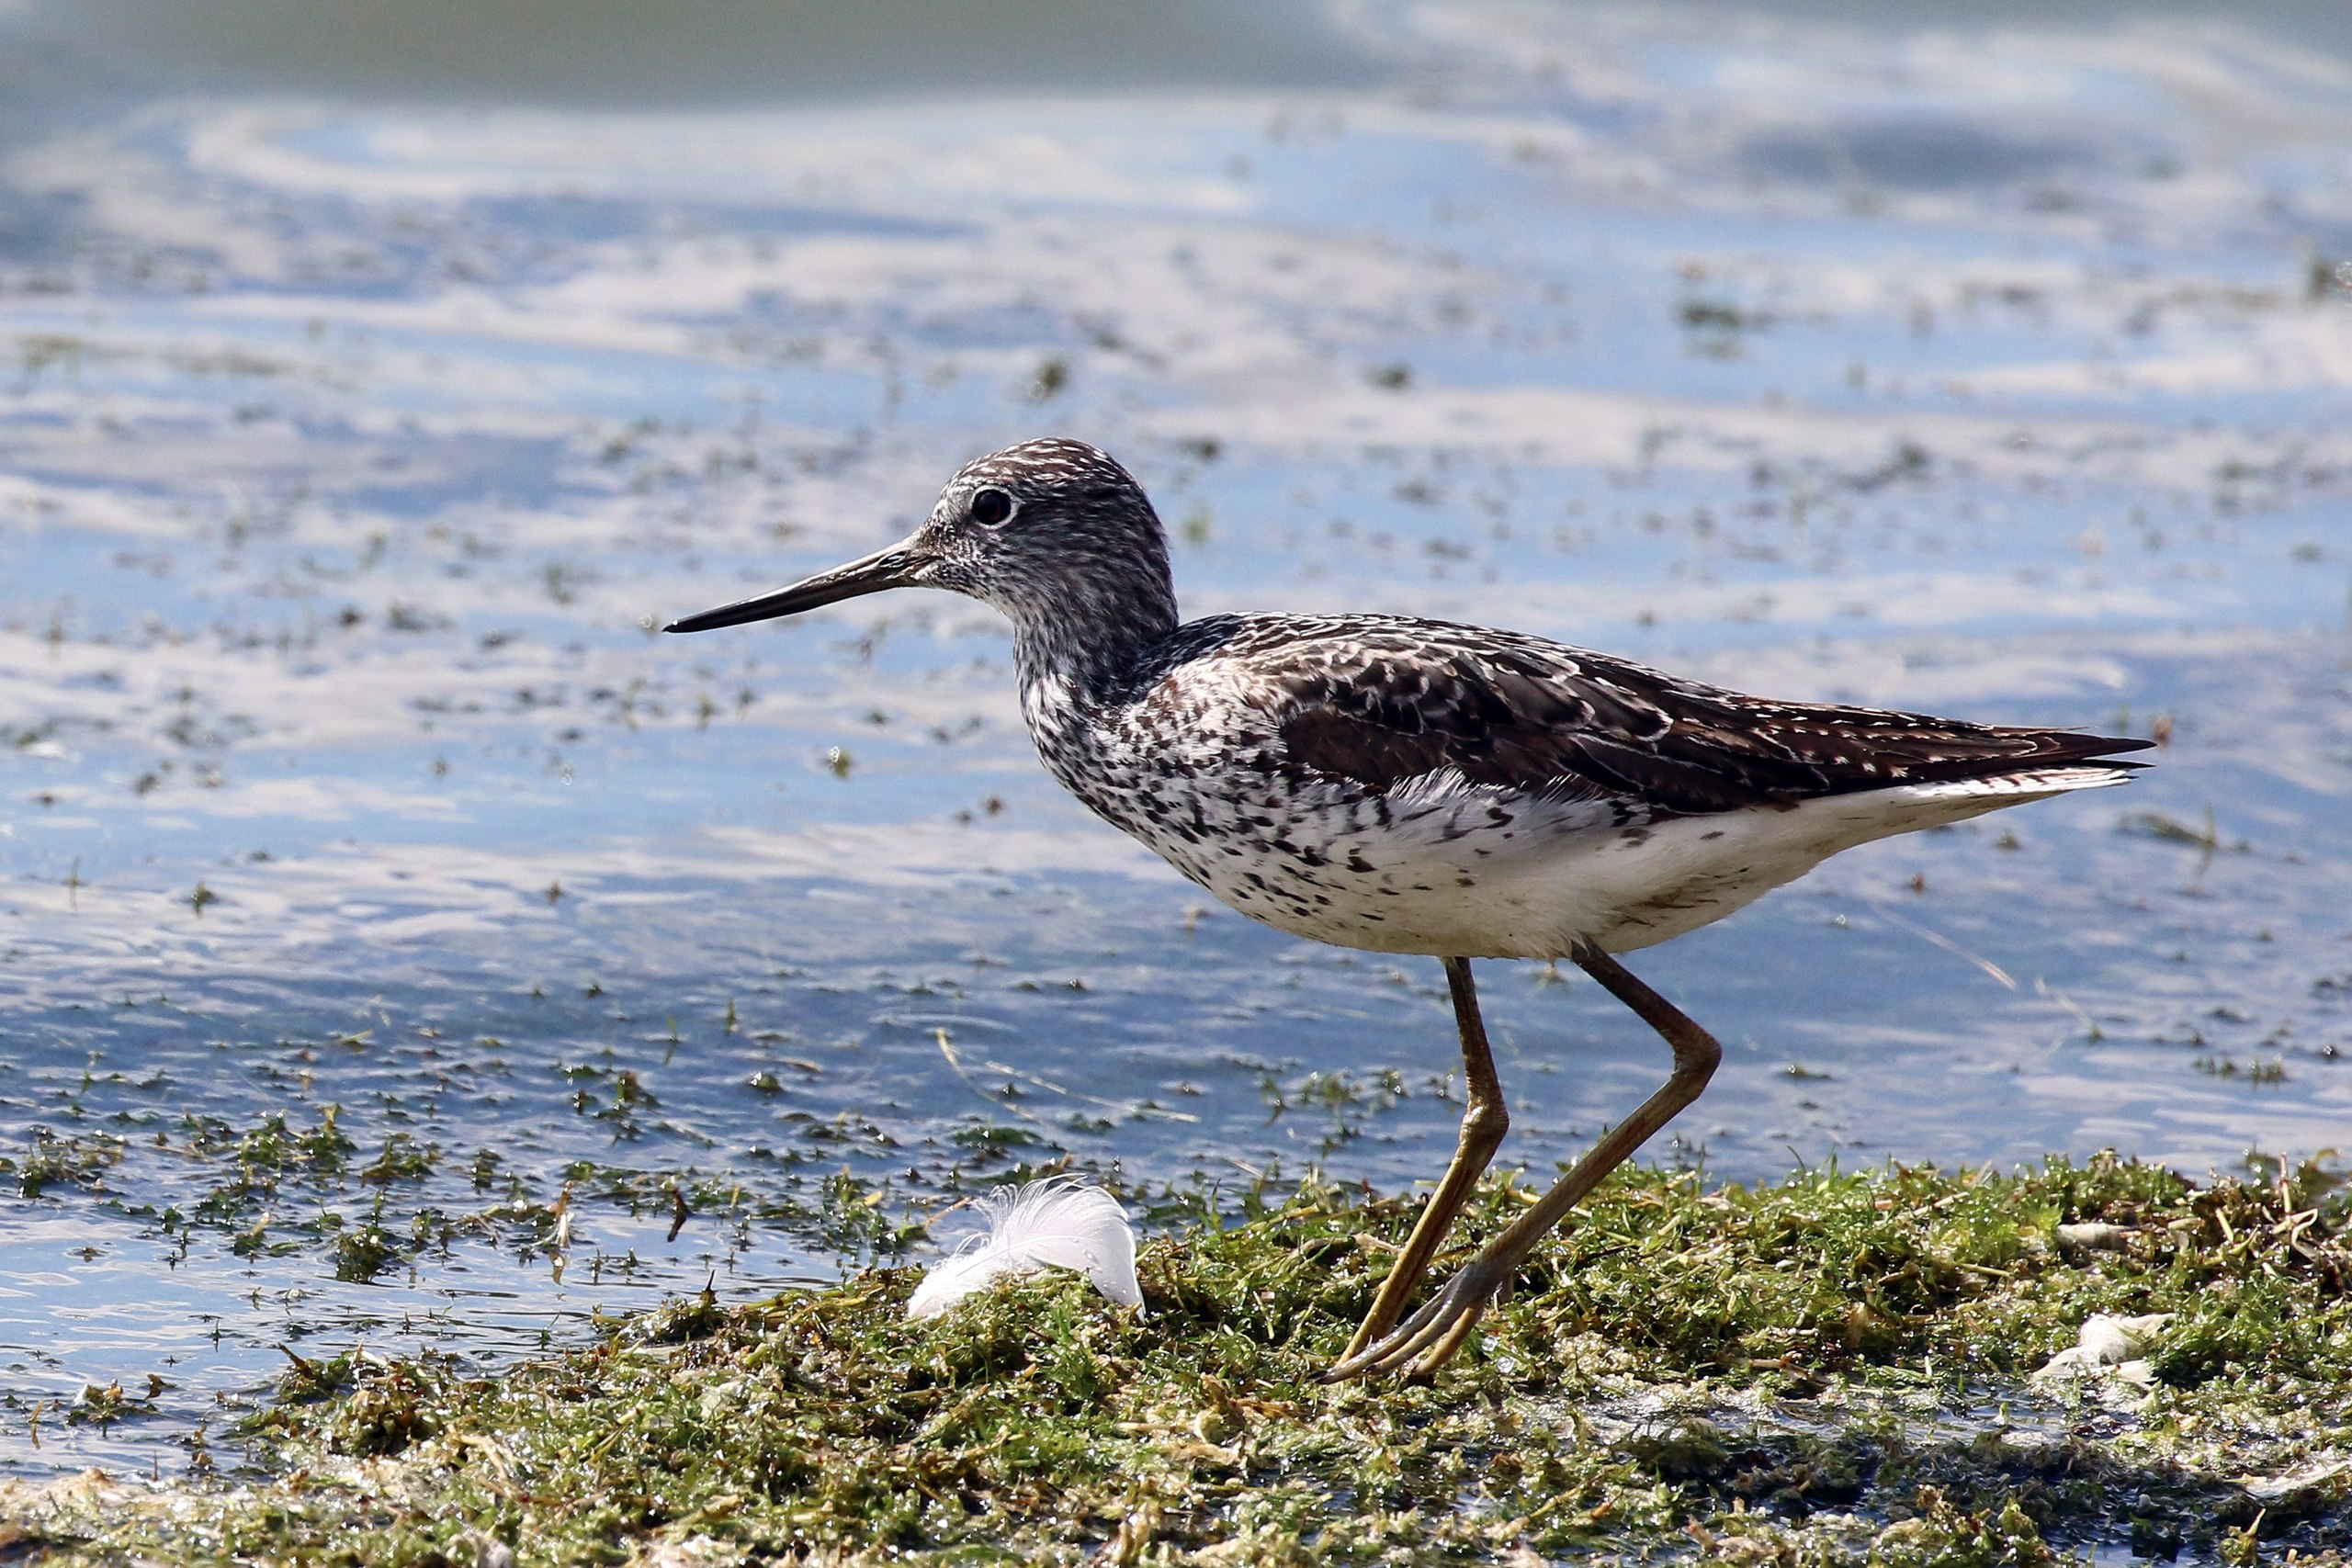
\includegraphics[width=0.8\linewidth, height=3cm, keepaspectratio]{Billeder/Dyr/Fugle/Vadefugle/hvidklire_sommer.jpg}\\[0.5em]
        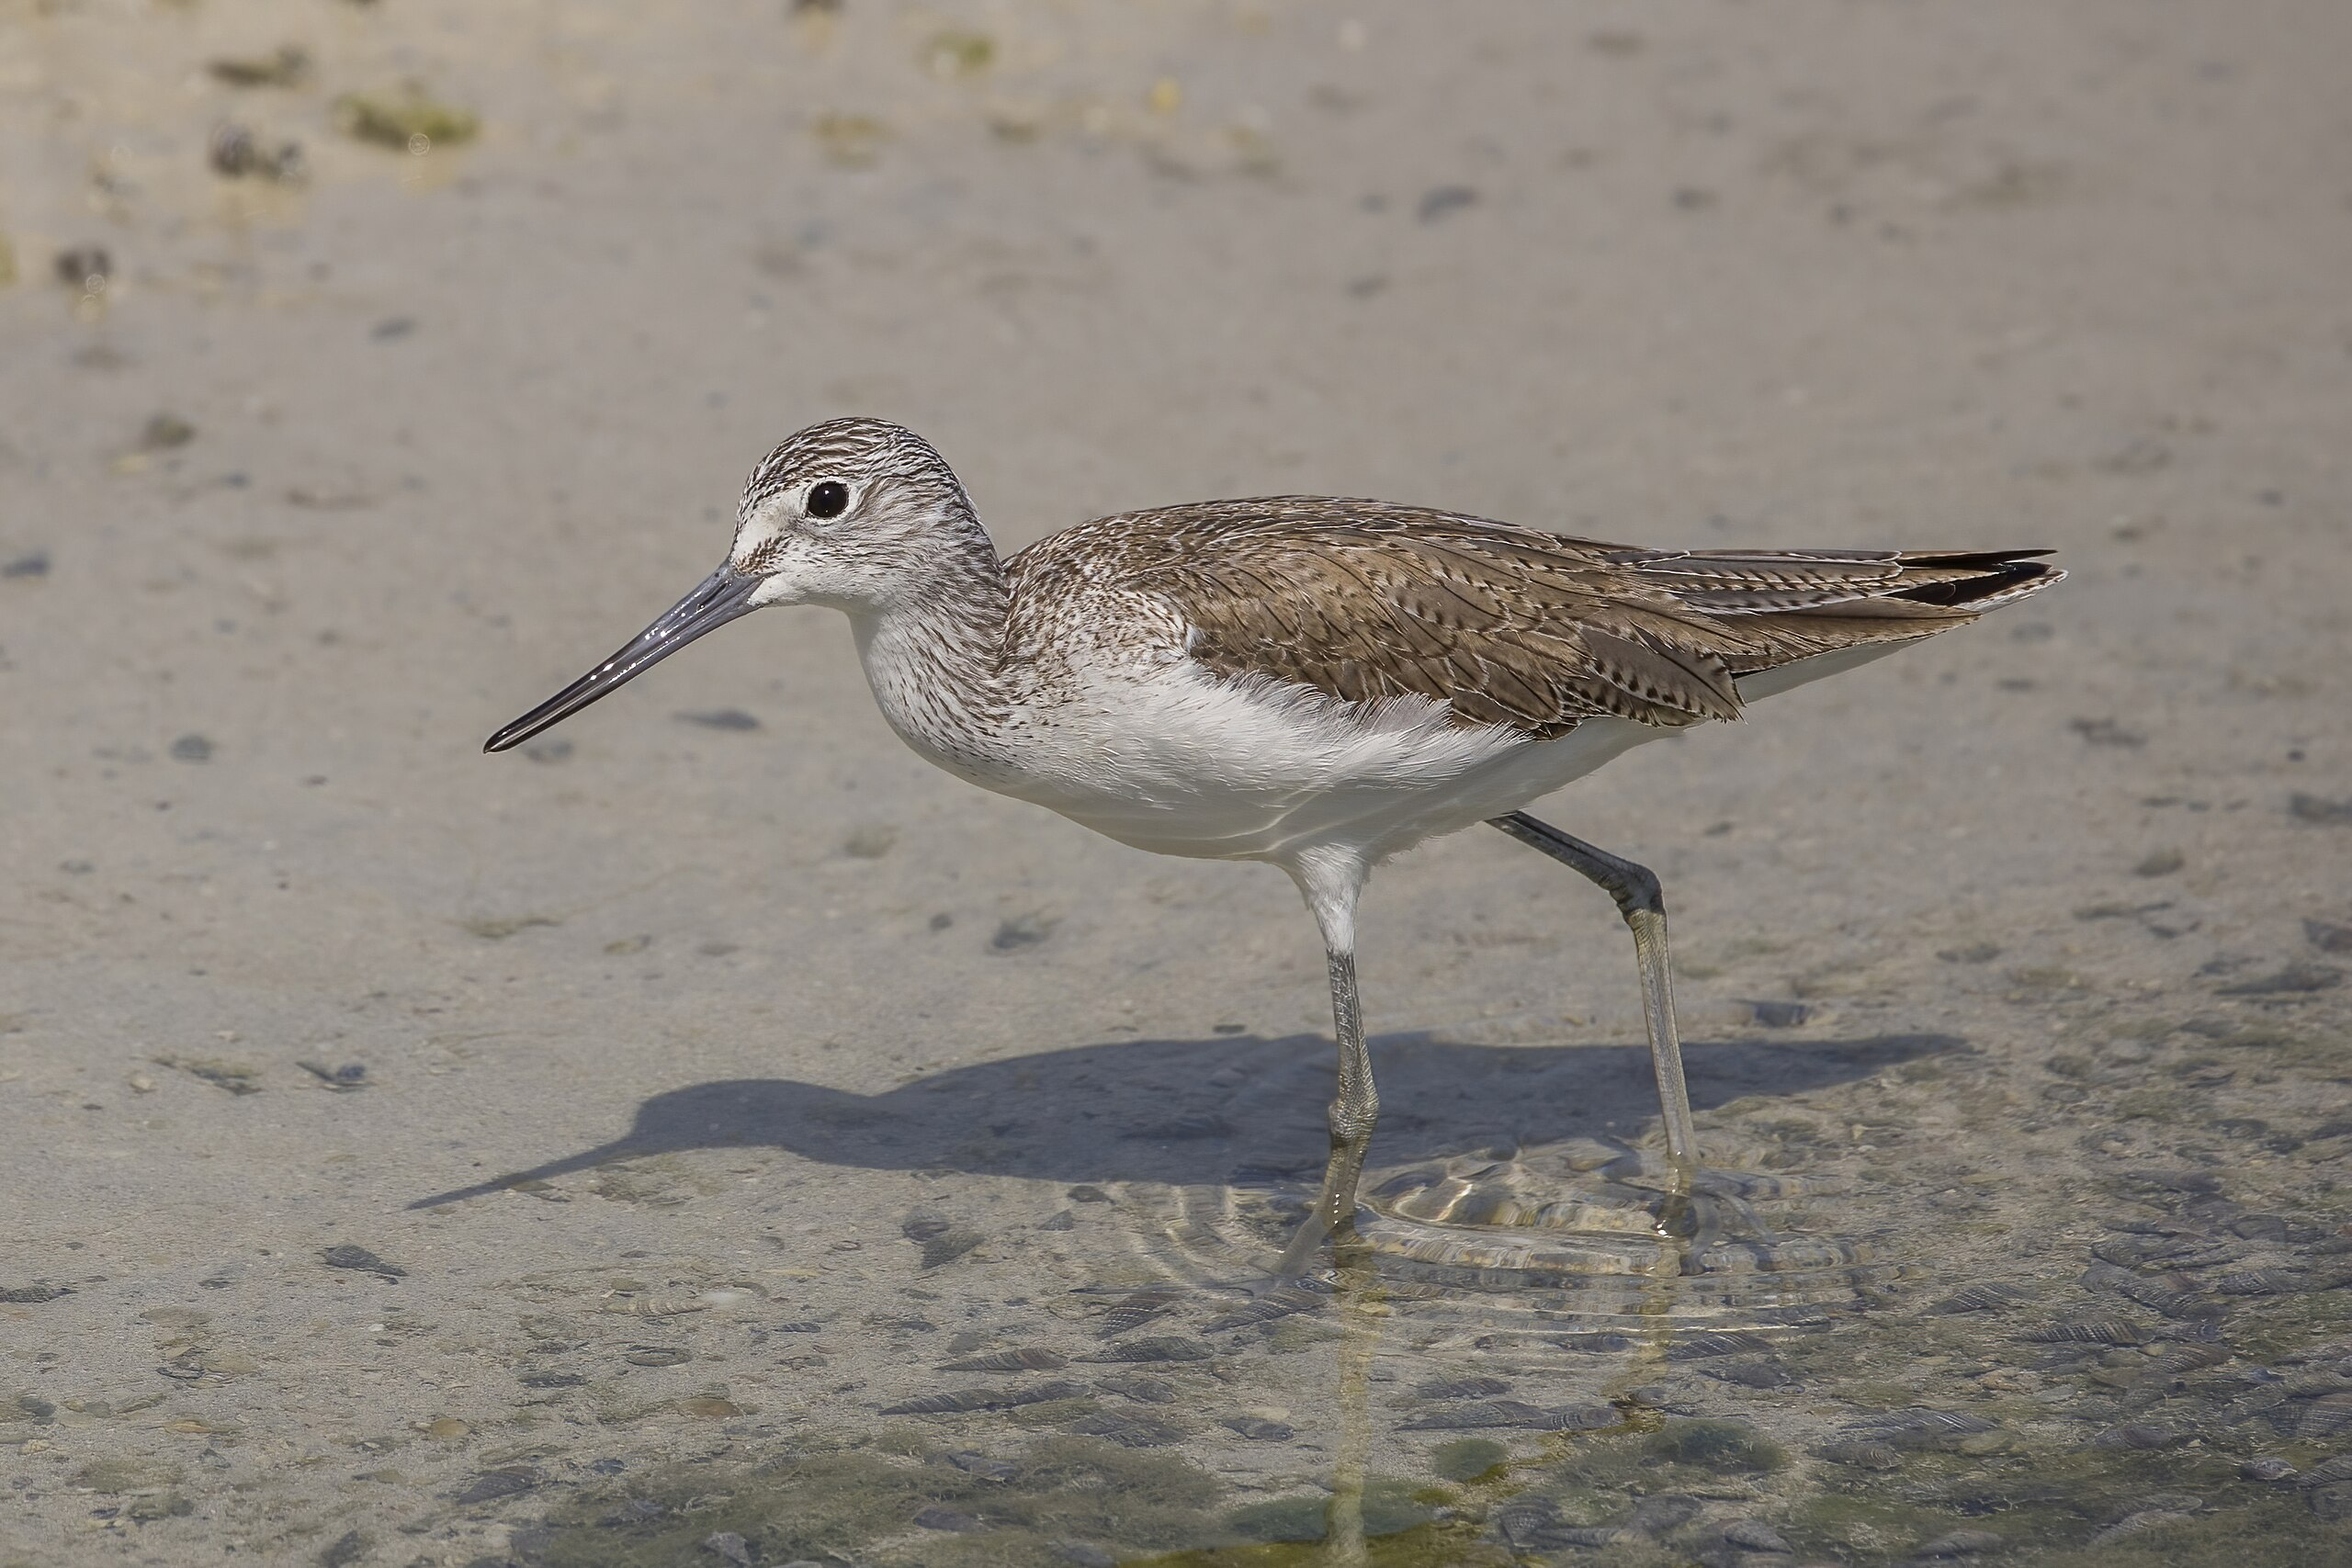
\includegraphics[width=0.8\linewidth, height=3cm, keepaspectratio]{Billeder/Dyr/Fugle/Vadefugle/hvidklire_vinter.jpg}%
      \end{minipage}
    }%
    \vspace{0.05em}
    \footnotesize Sommer fjerdragt øverst, vinter nederst
  \end{columns}
\end{frame}
\begin{frame}{%
\begin{minipage}[t]{0.85\textwidth}
Islandsk ryle
\end{minipage}%
\hfill
\begin{minipage}[t]{0.1\textwidth}
\raggedleft

\includegraphics[width=0.55cm, height=0.55cm, keepaspectratio]{Billeder/Ikoner/star.png}%
\end{minipage}%
}
\vspace{0.25em}
\begin{columns}[T]
% --- Venstre kolonne: Tekst ---
\column{0.55\textwidth}
\setlength{\parskip}{0.5em}
\small
\RaggedRight\textbf{\textit{Calidris canutus}} – Kortbenet kraftig vadefugl med kort næb\par

\textbf{Udseende:} \\
\quad –  Kort, mørkt næb og grågrønne ben  

% --- Højre kolonne: Et billede ---
\column{0.40\textwidth}
\centering
\fbox{%
\begin{minipage}{\linewidth}
\centering
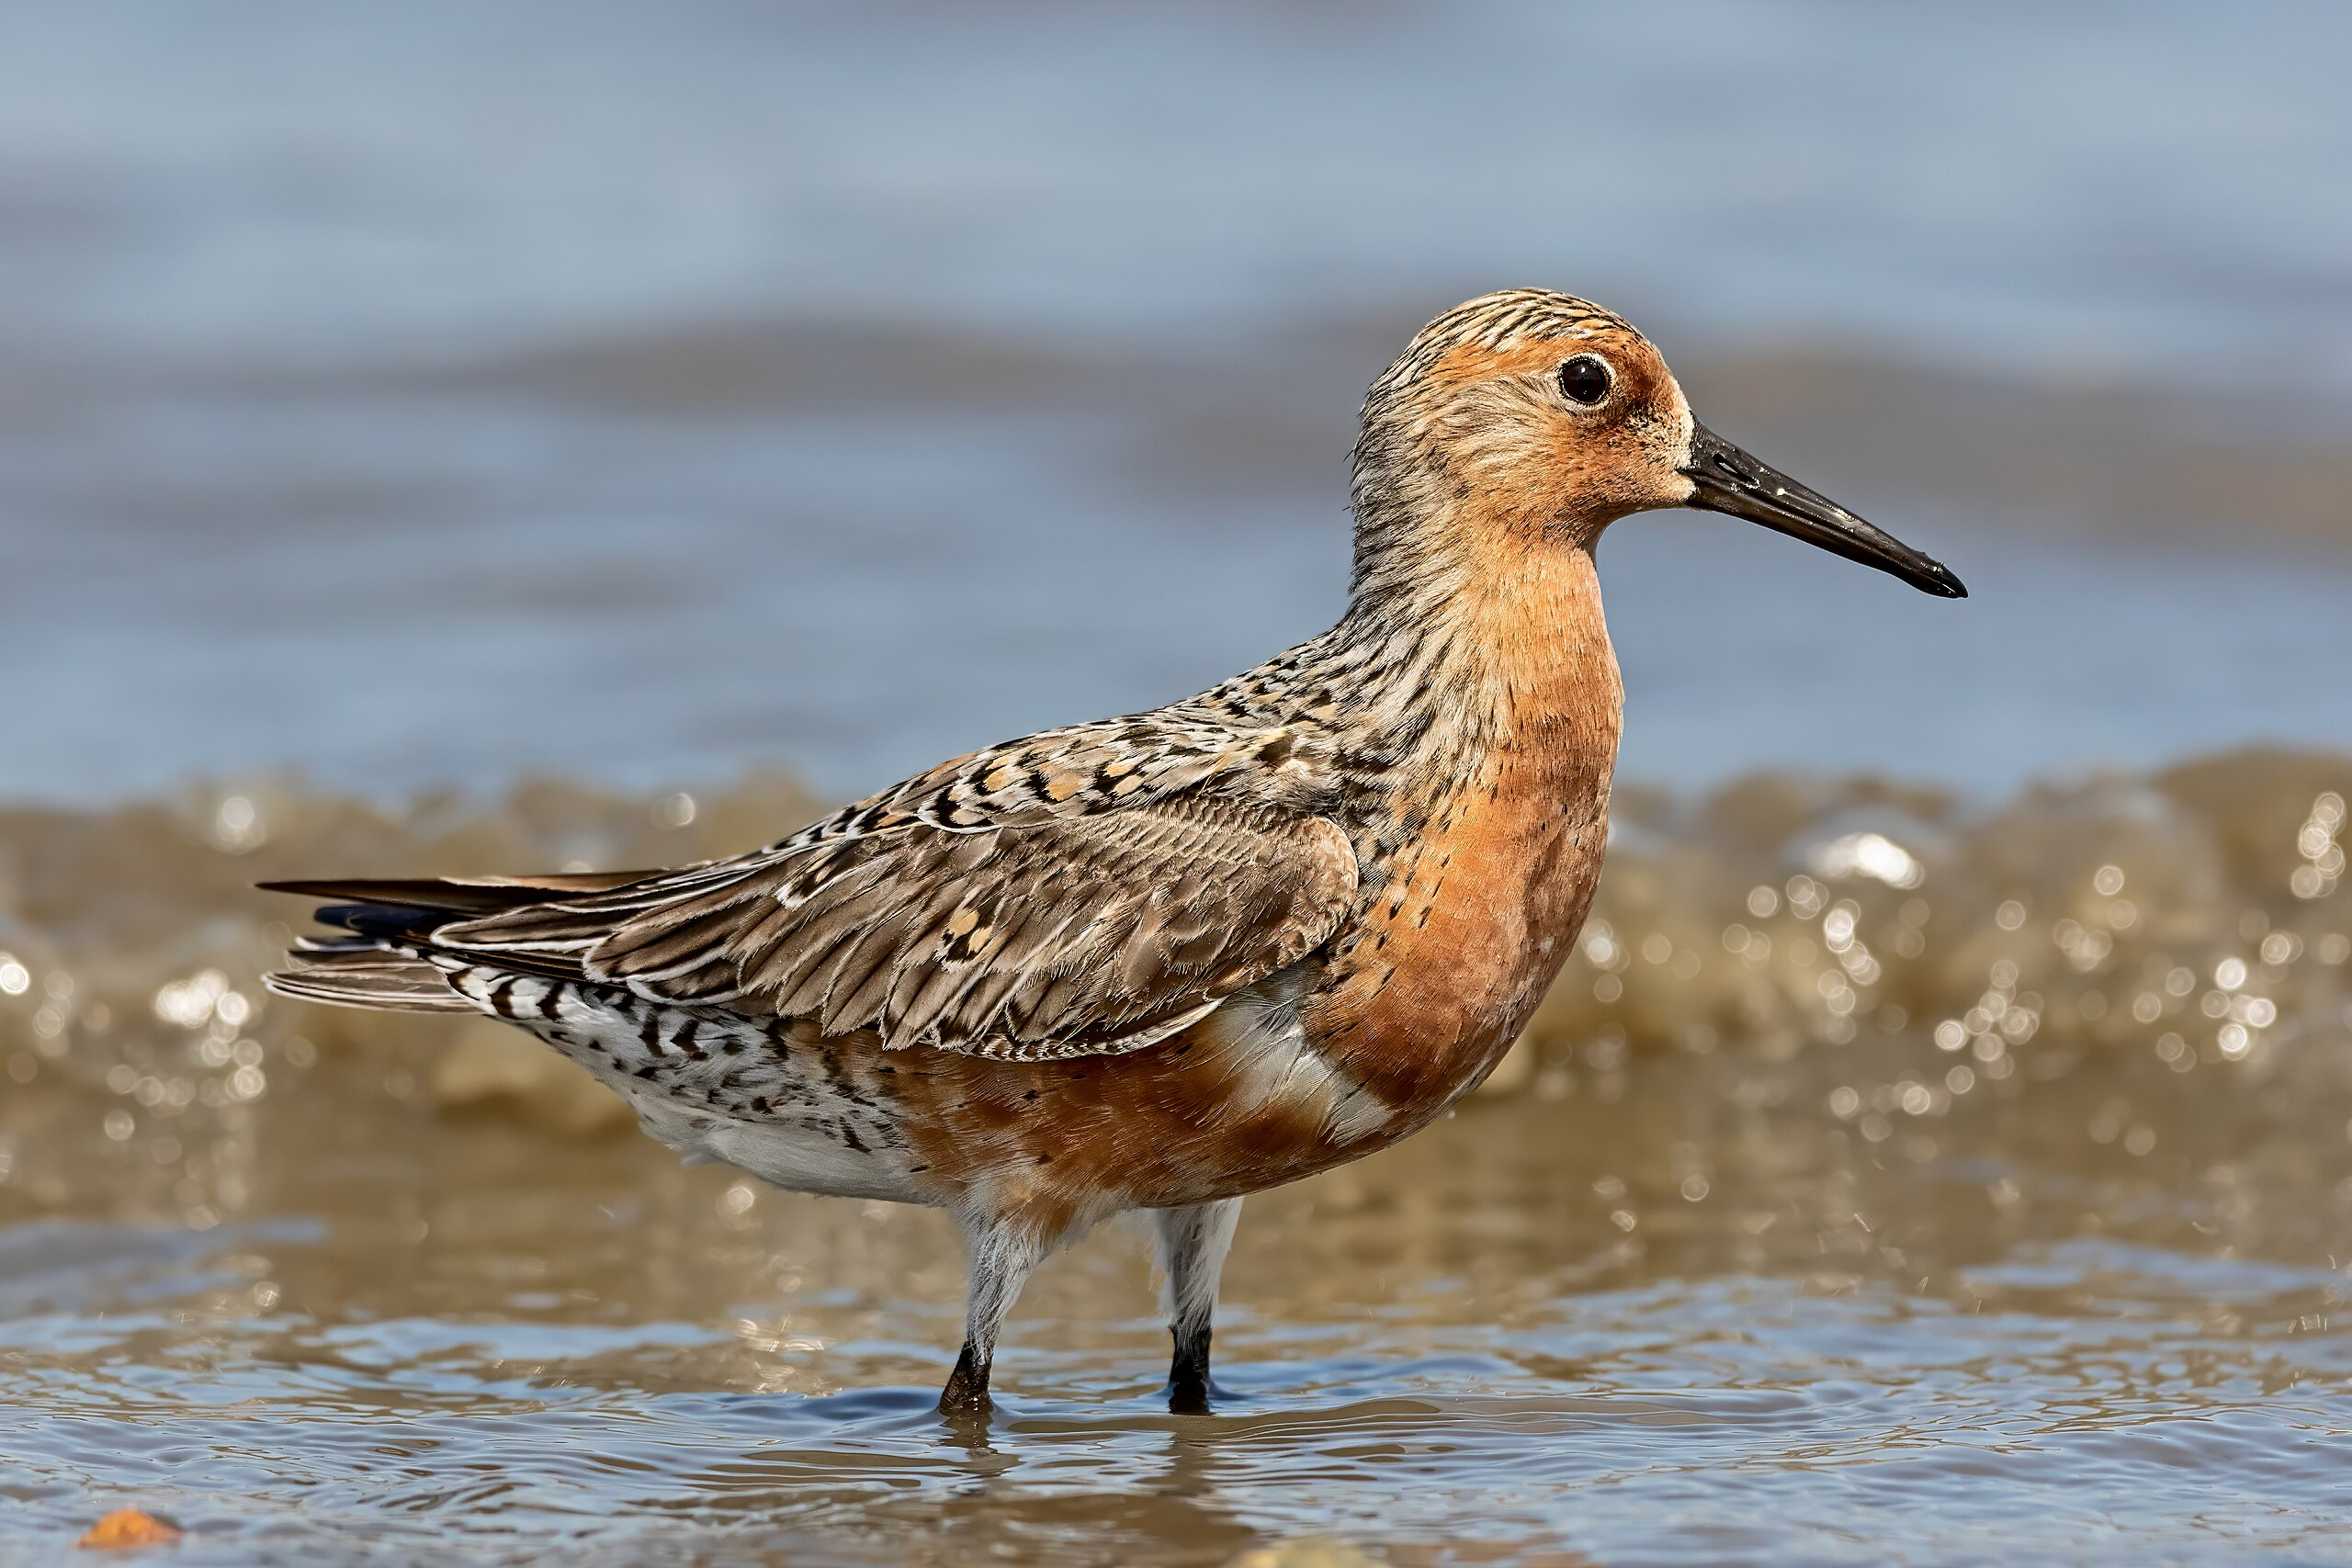
\includegraphics[width=0.8\linewidth, height=10cm, keepaspectratio]{Billeder/Dyr/Fugle/Vadefugle/islandsk_ryle.jpg}
\end{minipage}
}%
\end{columns}
\end{frame}



\begin{frame}{%
  \begin{minipage}[t]{0.85\textwidth}
    Brushane
  \end{minipage}%
  \hfill
  \begin{minipage}[t]{0.1\textwidth}
    \raggedleft
    
\includegraphics[width=0.55cm, height=0.55cm, keepaspectratio]{Billeder/Ikoner/star.png}%
  \end{minipage}%
} 
  \vspace{0.25em}
  \begin{columns}[T]
    % --- Venstre kolonne: Tekst ---
    \column{0.55\textwidth}
    \setlength{\parskip}{0.5em}
    \small
    \RaggedRight\textbf{\textit{Calidris pugnax}} – stor vadefugl som tilhører sneppefuglene \par

    \textbf{Udseende:} \\
    \quad – Kort svagt nedadbøjet næb. Giraf-hals. Uproportionelt lille hoved ift. krop. 

    

    % --- Højre kolonne: To billeder stablet over hinanden ---
    \column{0.40\textwidth}
    \centering
    \fbox{%
      \begin{minipage}{\linewidth}
        \centering
        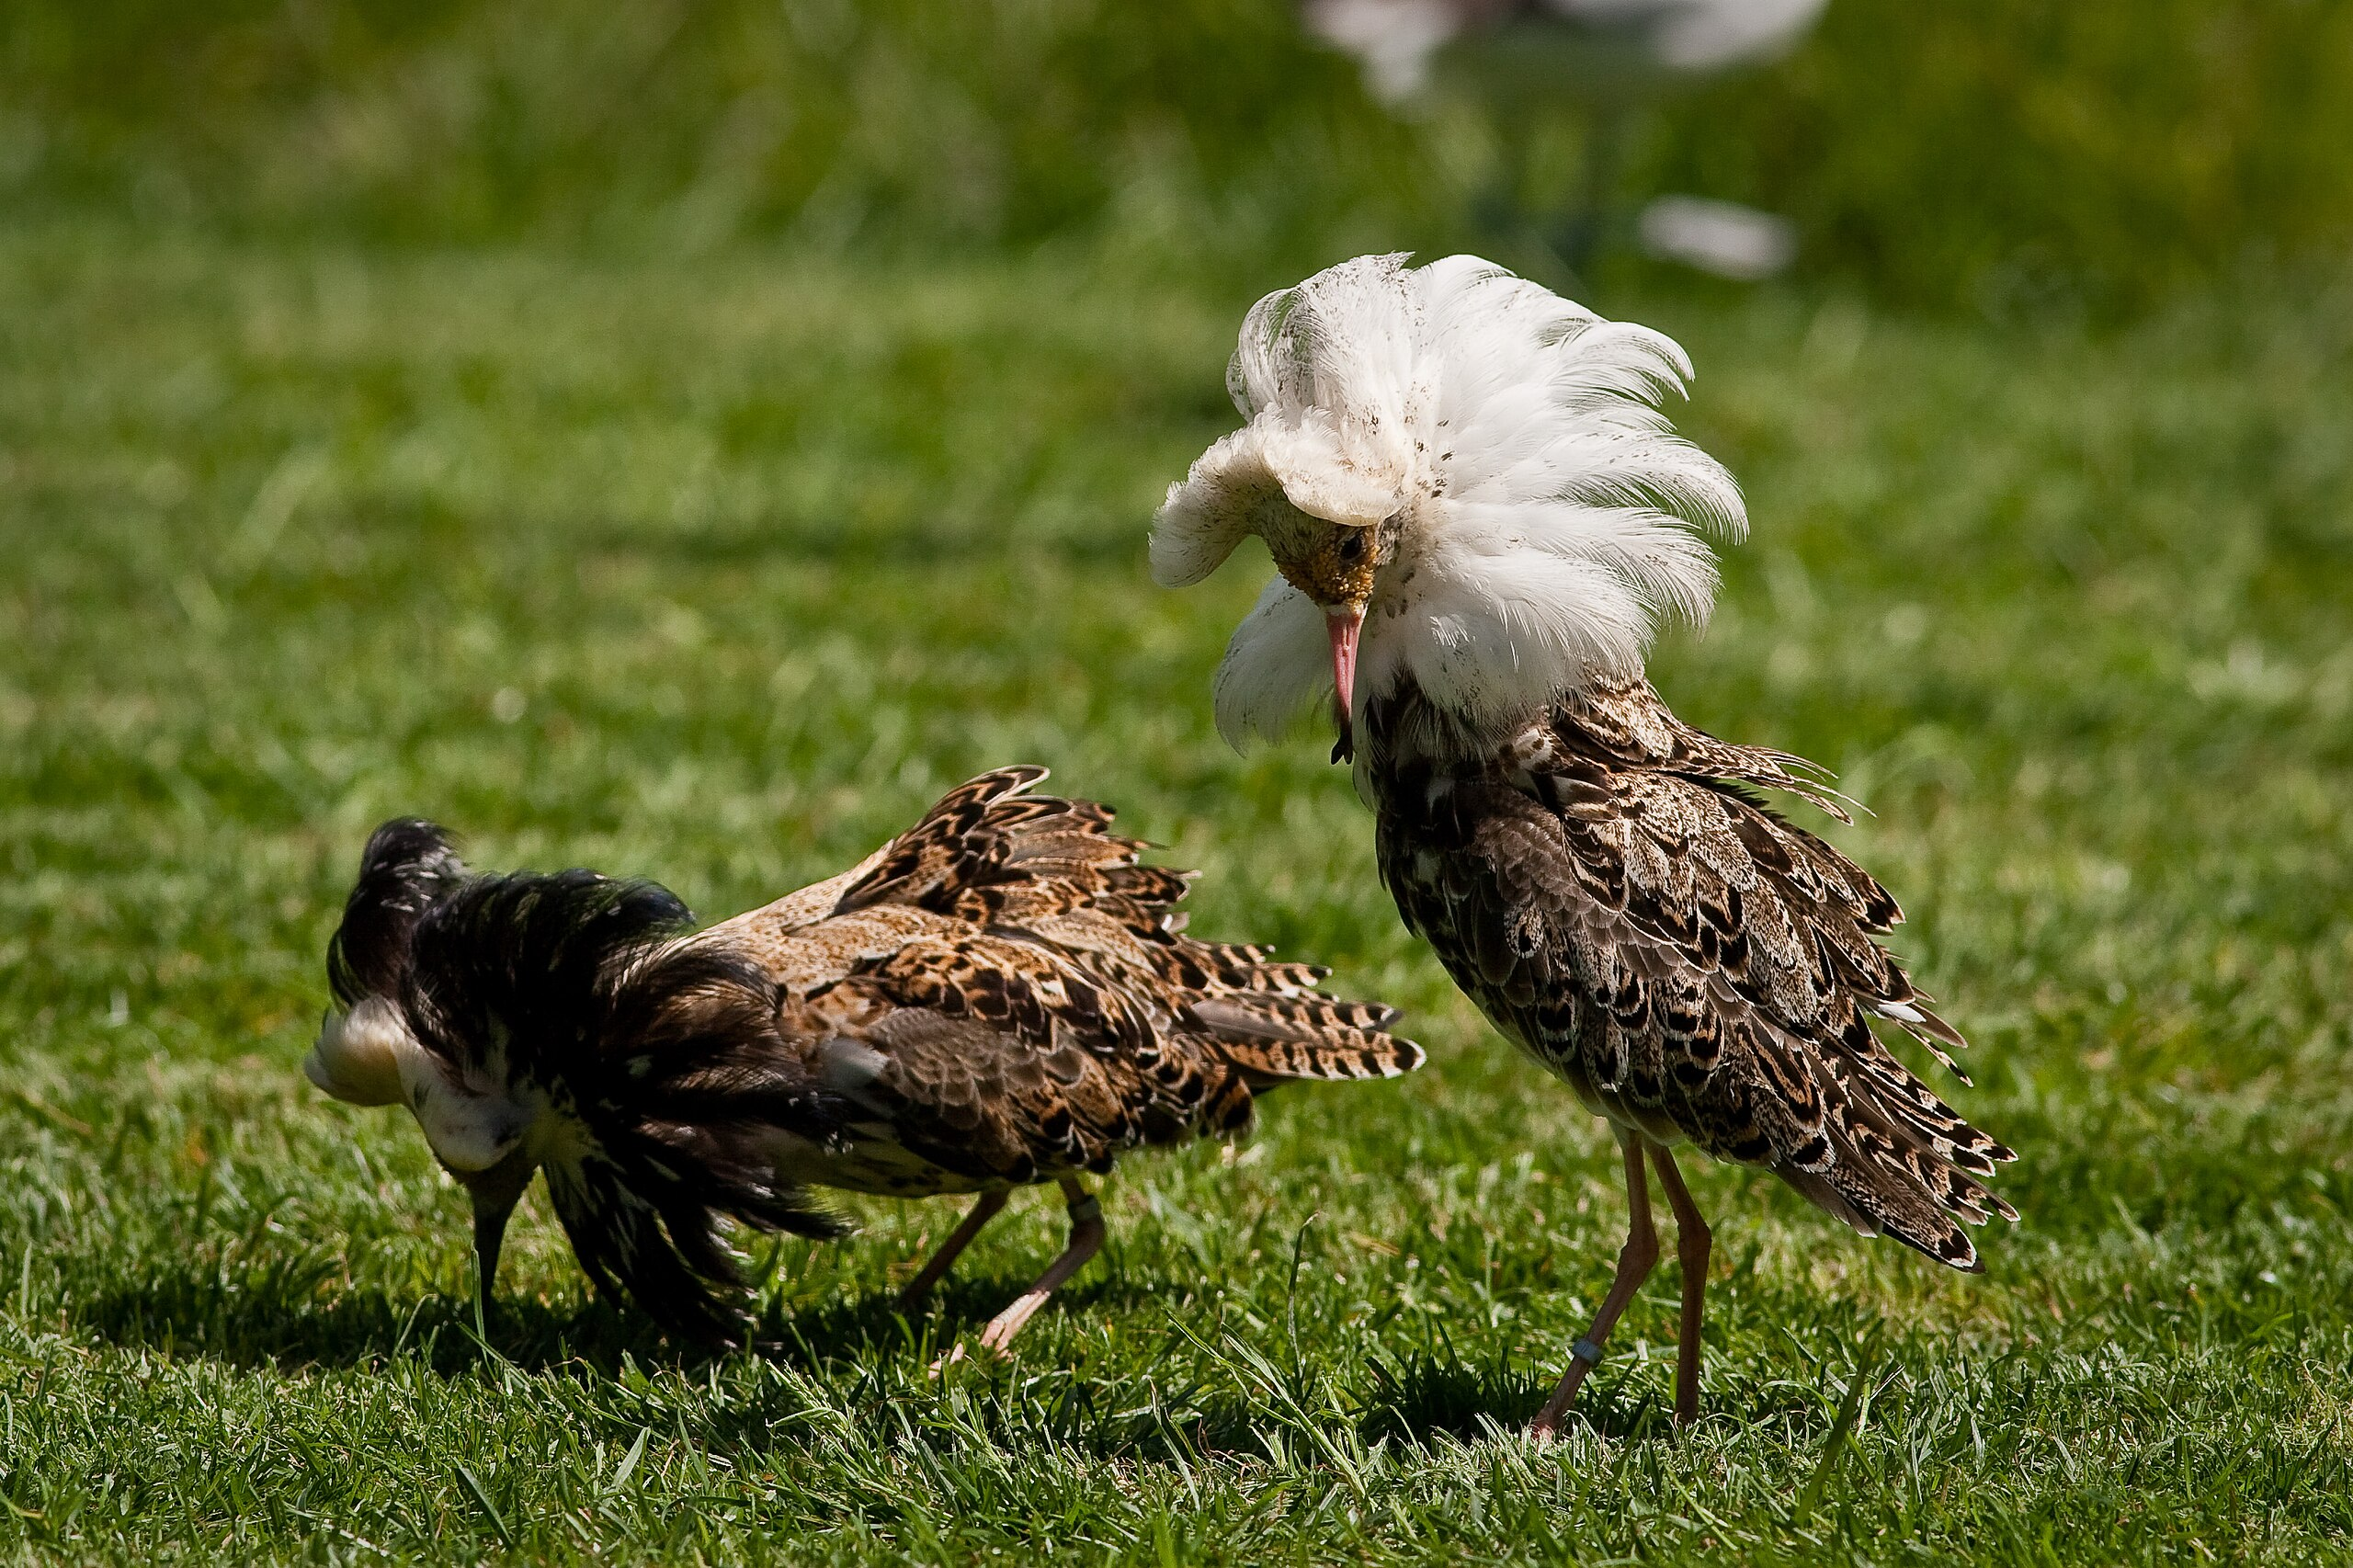
\includegraphics[width=0.8\linewidth, height=3cm, keepaspectratio]{Billeder/Dyr/Fugle/Vadefugle/brushane_han.jpg}\\[0.5em]
        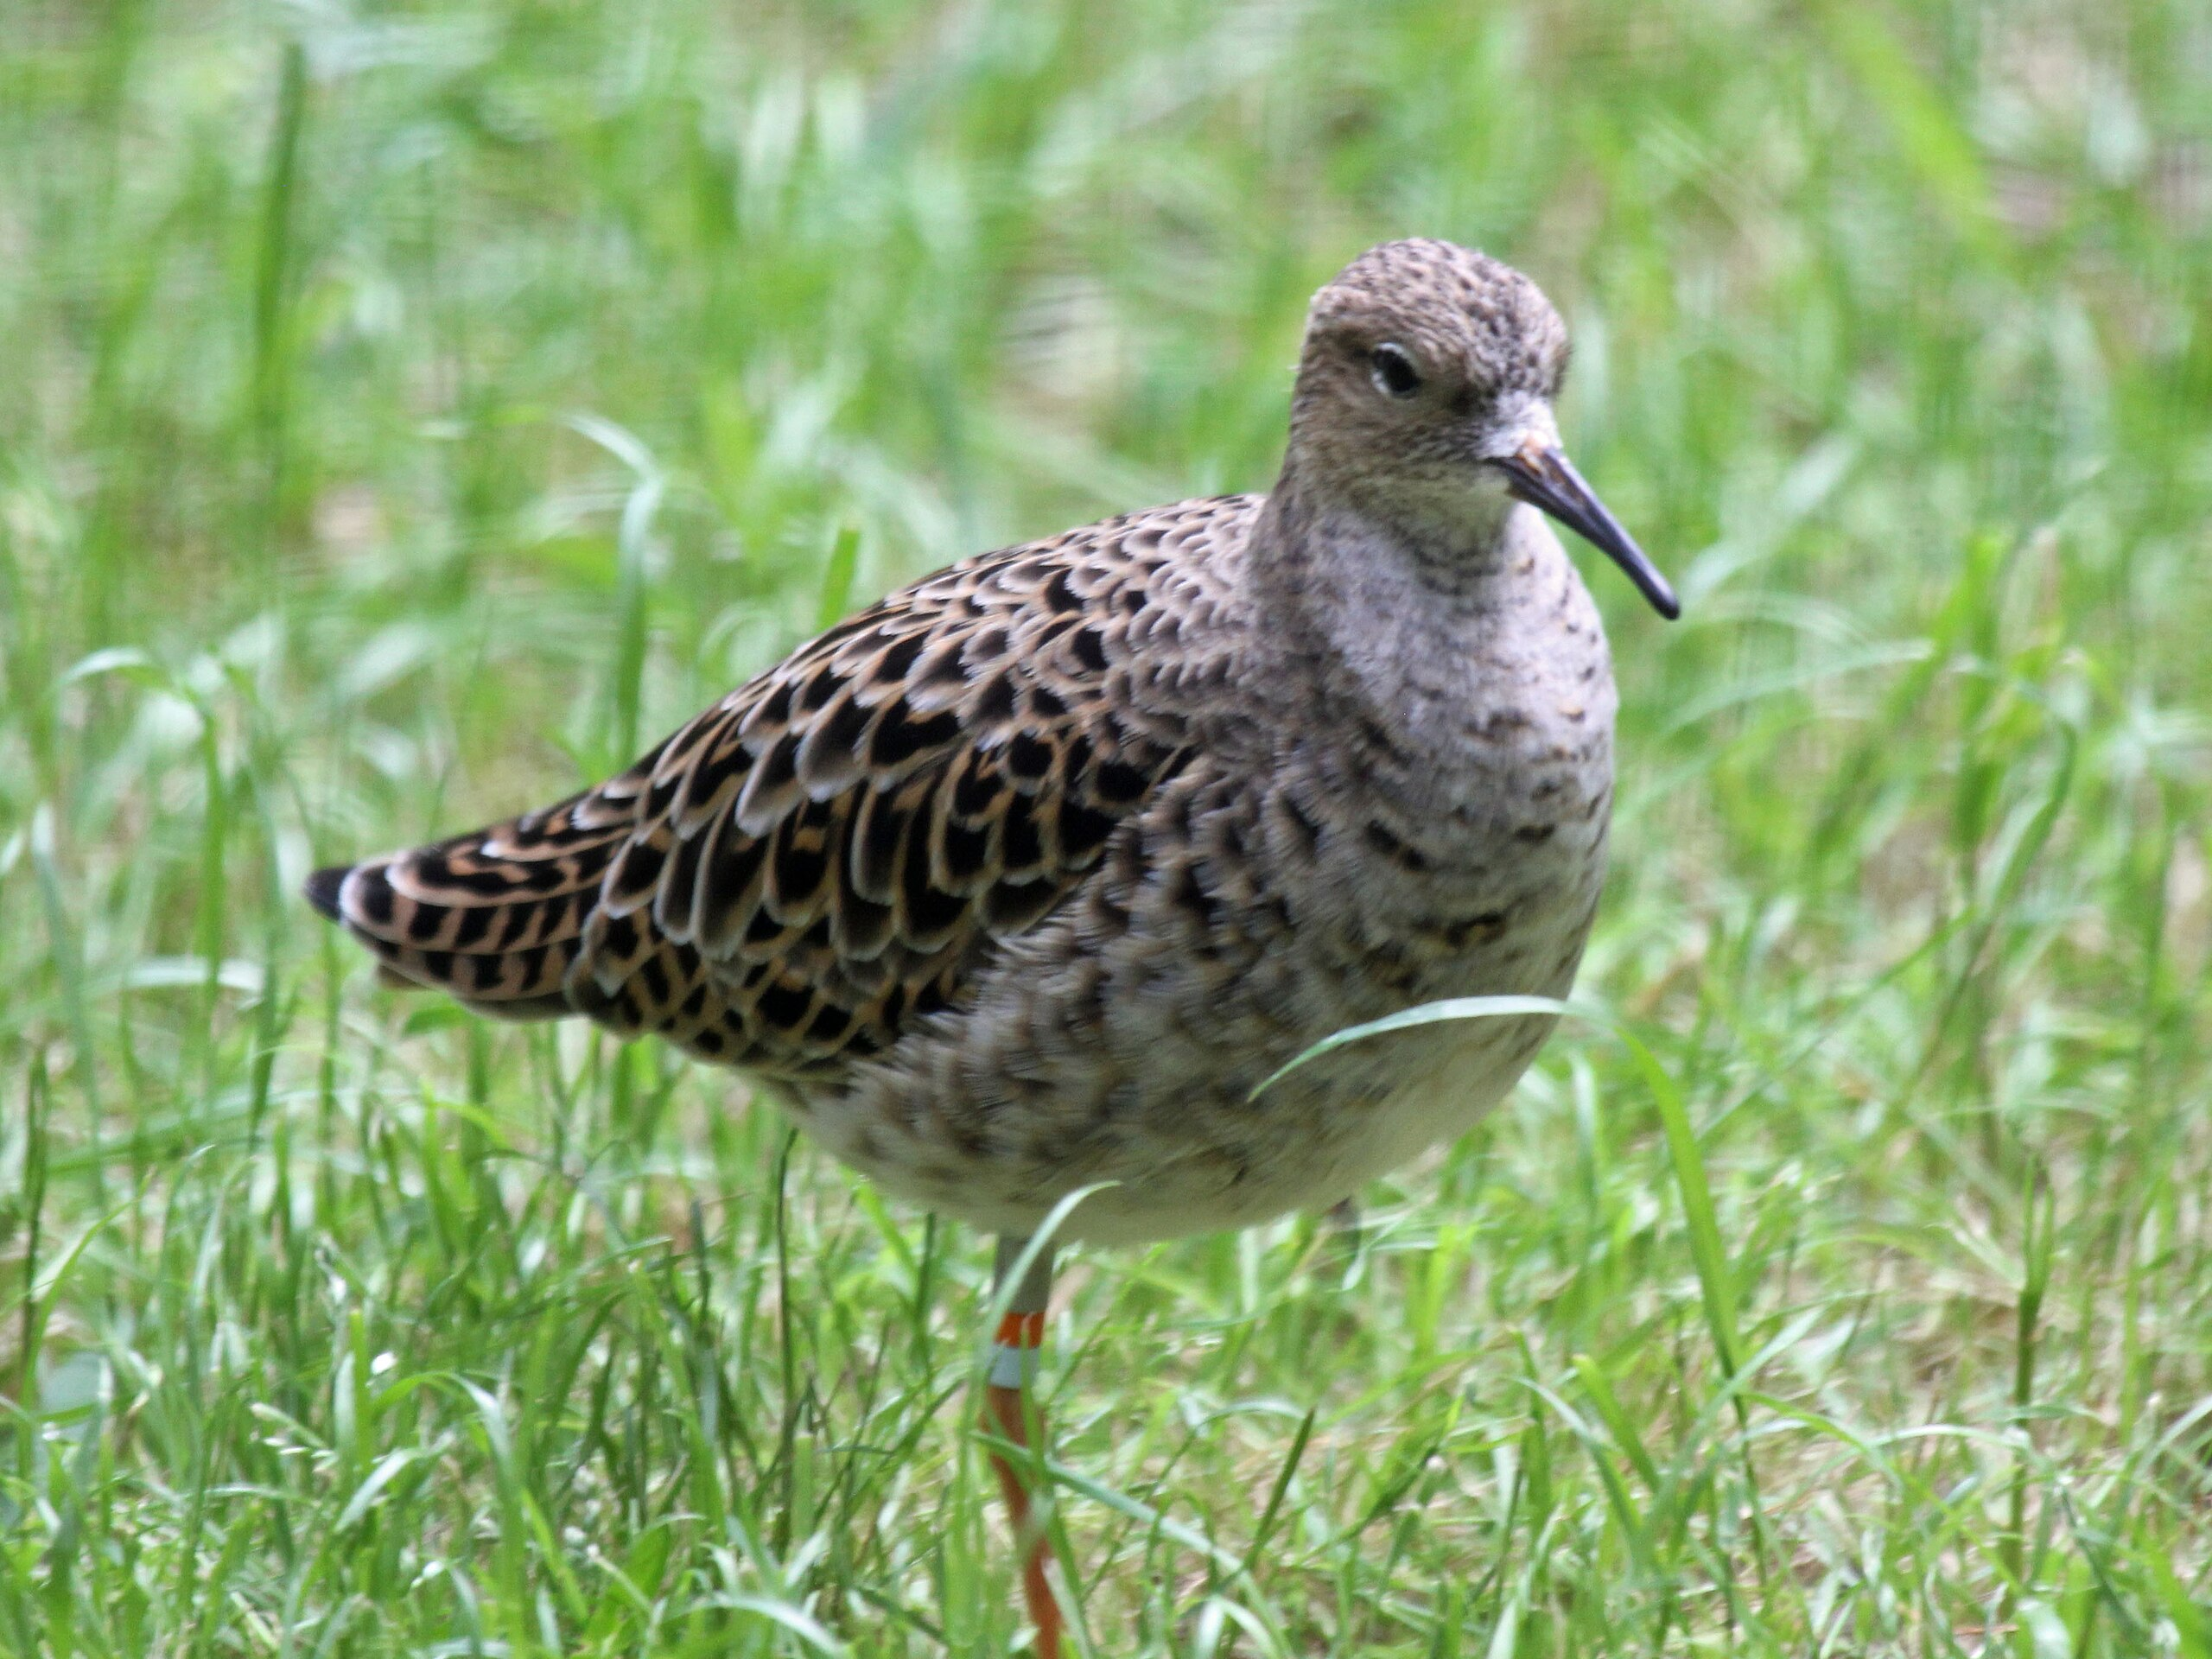
\includegraphics[width=0.8\linewidth, height=3cm, keepaspectratio]{Billeder/Dyr/Fugle/Vadefugle/brushane_hun.jpg}%
      \end{minipage}
    }%
    \vspace{0.05em}
    \footnotesize Han øverst, hun nederst
  \end{columns}
\end{frame}
\begin{frame}{%
\begin{minipage}[t]{0.85\textwidth}
Dobbeltbekkasin
\end{minipage}%
\hfill
\begin{minipage}[t]{0.1\textwidth}
\raggedleft

\includegraphics[width=0.5cm, height=0.5cm, keepaspectratio]{Billeder/Ikoner/star.png}%
\hspace{0.2em}%

\includegraphics[width=0.5cm, height=0.5cm, keepaspectratio]{Billeder/Ikoner/star.png}
\end{minipage}%
}
\vspace{0.25em}
\begin{columns}[T]
% --- Venstre kolonne: Tekst ---
\column{0.55\textwidth}
\setlength{\parskip}{0.5em}
\small
\RaggedRight\textbf{\textit{Gallinago gallinago}} – På størrelse med solsort med meget langt næb\par 

\textbf{Udseende:} \\
\quad –  Brun ryg med gule længdestriber. Mørkebrun isse med gule issestribe. Næb mere end dobbelt så langt som hoved \par

\textbf{Levesteder:} \\
\quad – Engarealer, marsk og moser \par

\textbf{Føde:} \\
\quad – Insekter, biller, larver, orme \par

\textbf{Udbredelse:} \\
\quad – I hele landet \par

\textbf{Træk/standfugl} \\
\quad – Begge \par

% --- Højre kolonne: Kun ét billede (Hannen) ---
\column{0.40\textwidth}
\centering
\fbox{%
\begin{minipage}{\linewidth}
\centering
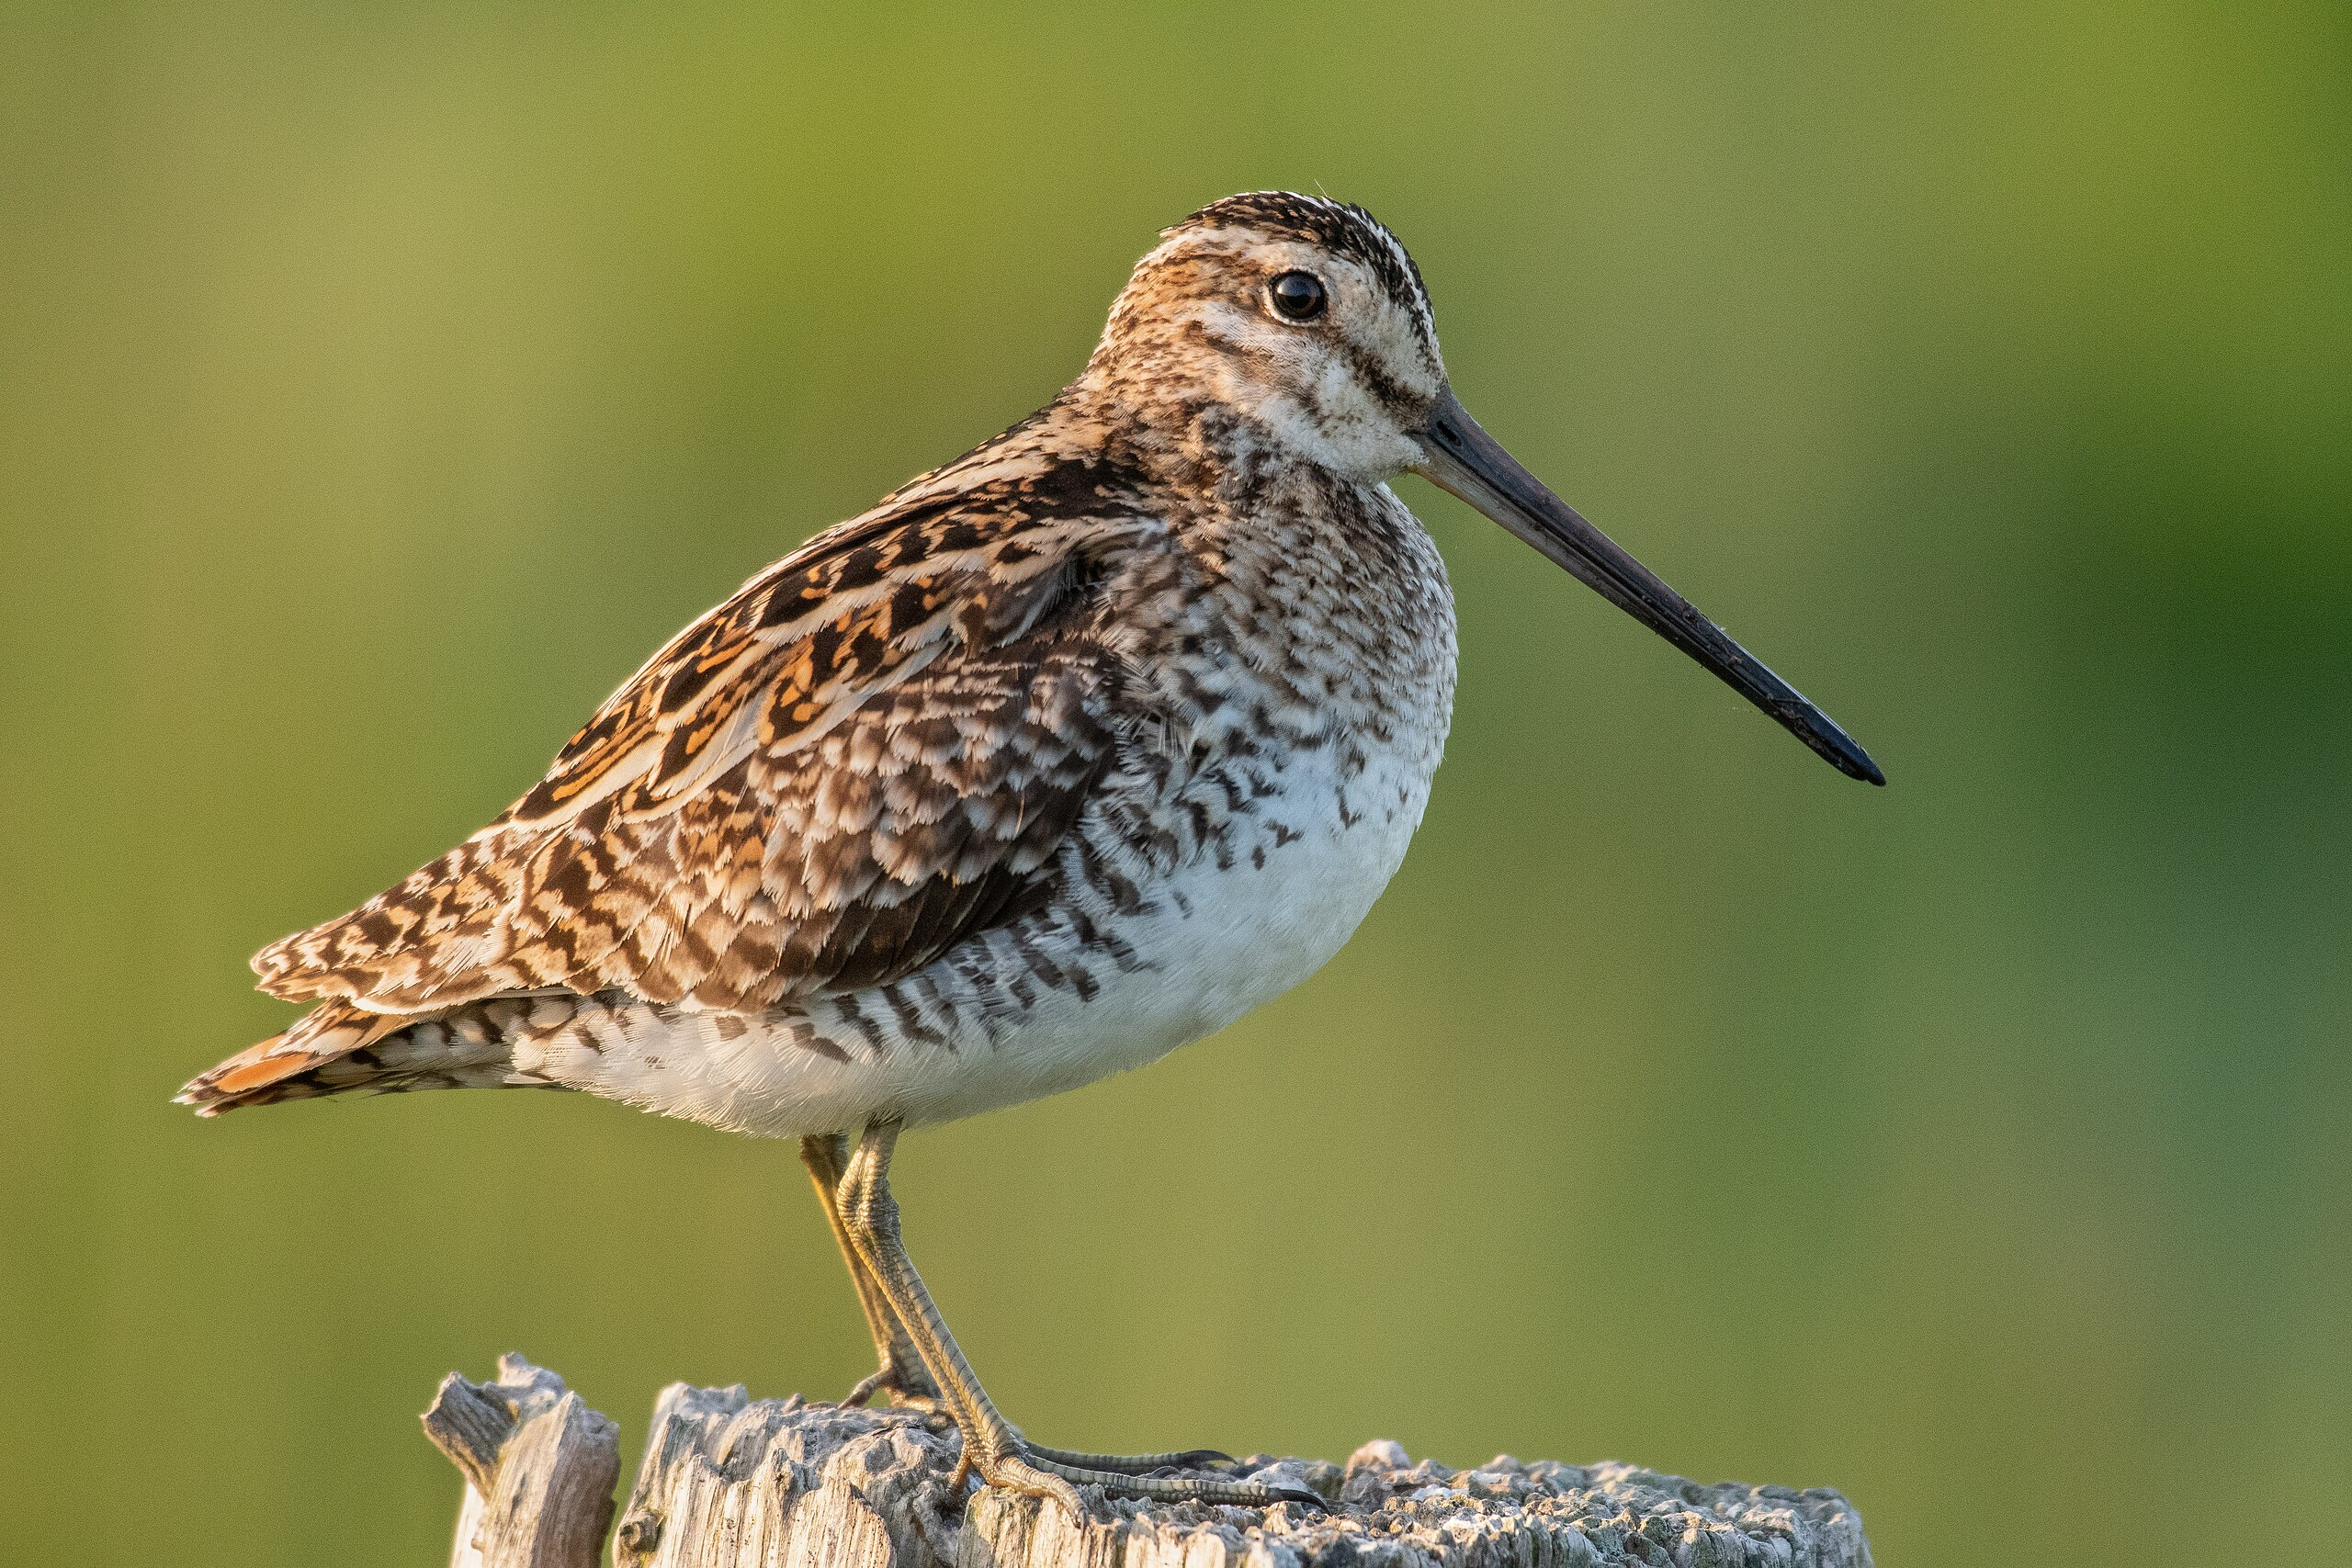
\includegraphics[width=0.8\linewidth, height=6.5cm, keepaspectratio]{Billeder/Dyr/Fugle/Vadefugle/dobbelt_bekksasin.jpg}%
\end{minipage}
}%
\end{columns}
\end{frame}
\begin{frame}{%
\begin{minipage}[t]{0.85\textwidth}
Enkeltbekkasin
\end{minipage}%
\hfill
\begin{minipage}[t]{0.1\textwidth}
\raggedleft

\includegraphics[width=0.55cm, height=0.55cm, keepaspectratio]{Billeder/Ikoner/star.png}%
\end{minipage}%
}
\vspace{0.25em}
\begin{columns}[T]
% --- Venstre kolonne: Tekst ---
\column{0.55\textwidth}
\setlength{\parskip}{0.5em}
\small
\RaggedRight\textbf{\textit{Lymnocryptes minimus}} – Ligner dobbeltbekkasin men er kun halv størrelse\par

\textbf{Udseende:} \\
\quad –  Gulige længdestriber, brun isse uden midterstribe. Kort næb kun lidt længere end hovedet.  

% --- Højre kolonne: Et billede ---
\column{0.40\textwidth}
\centering
\fbox{%
\begin{minipage}{\linewidth}
\centering
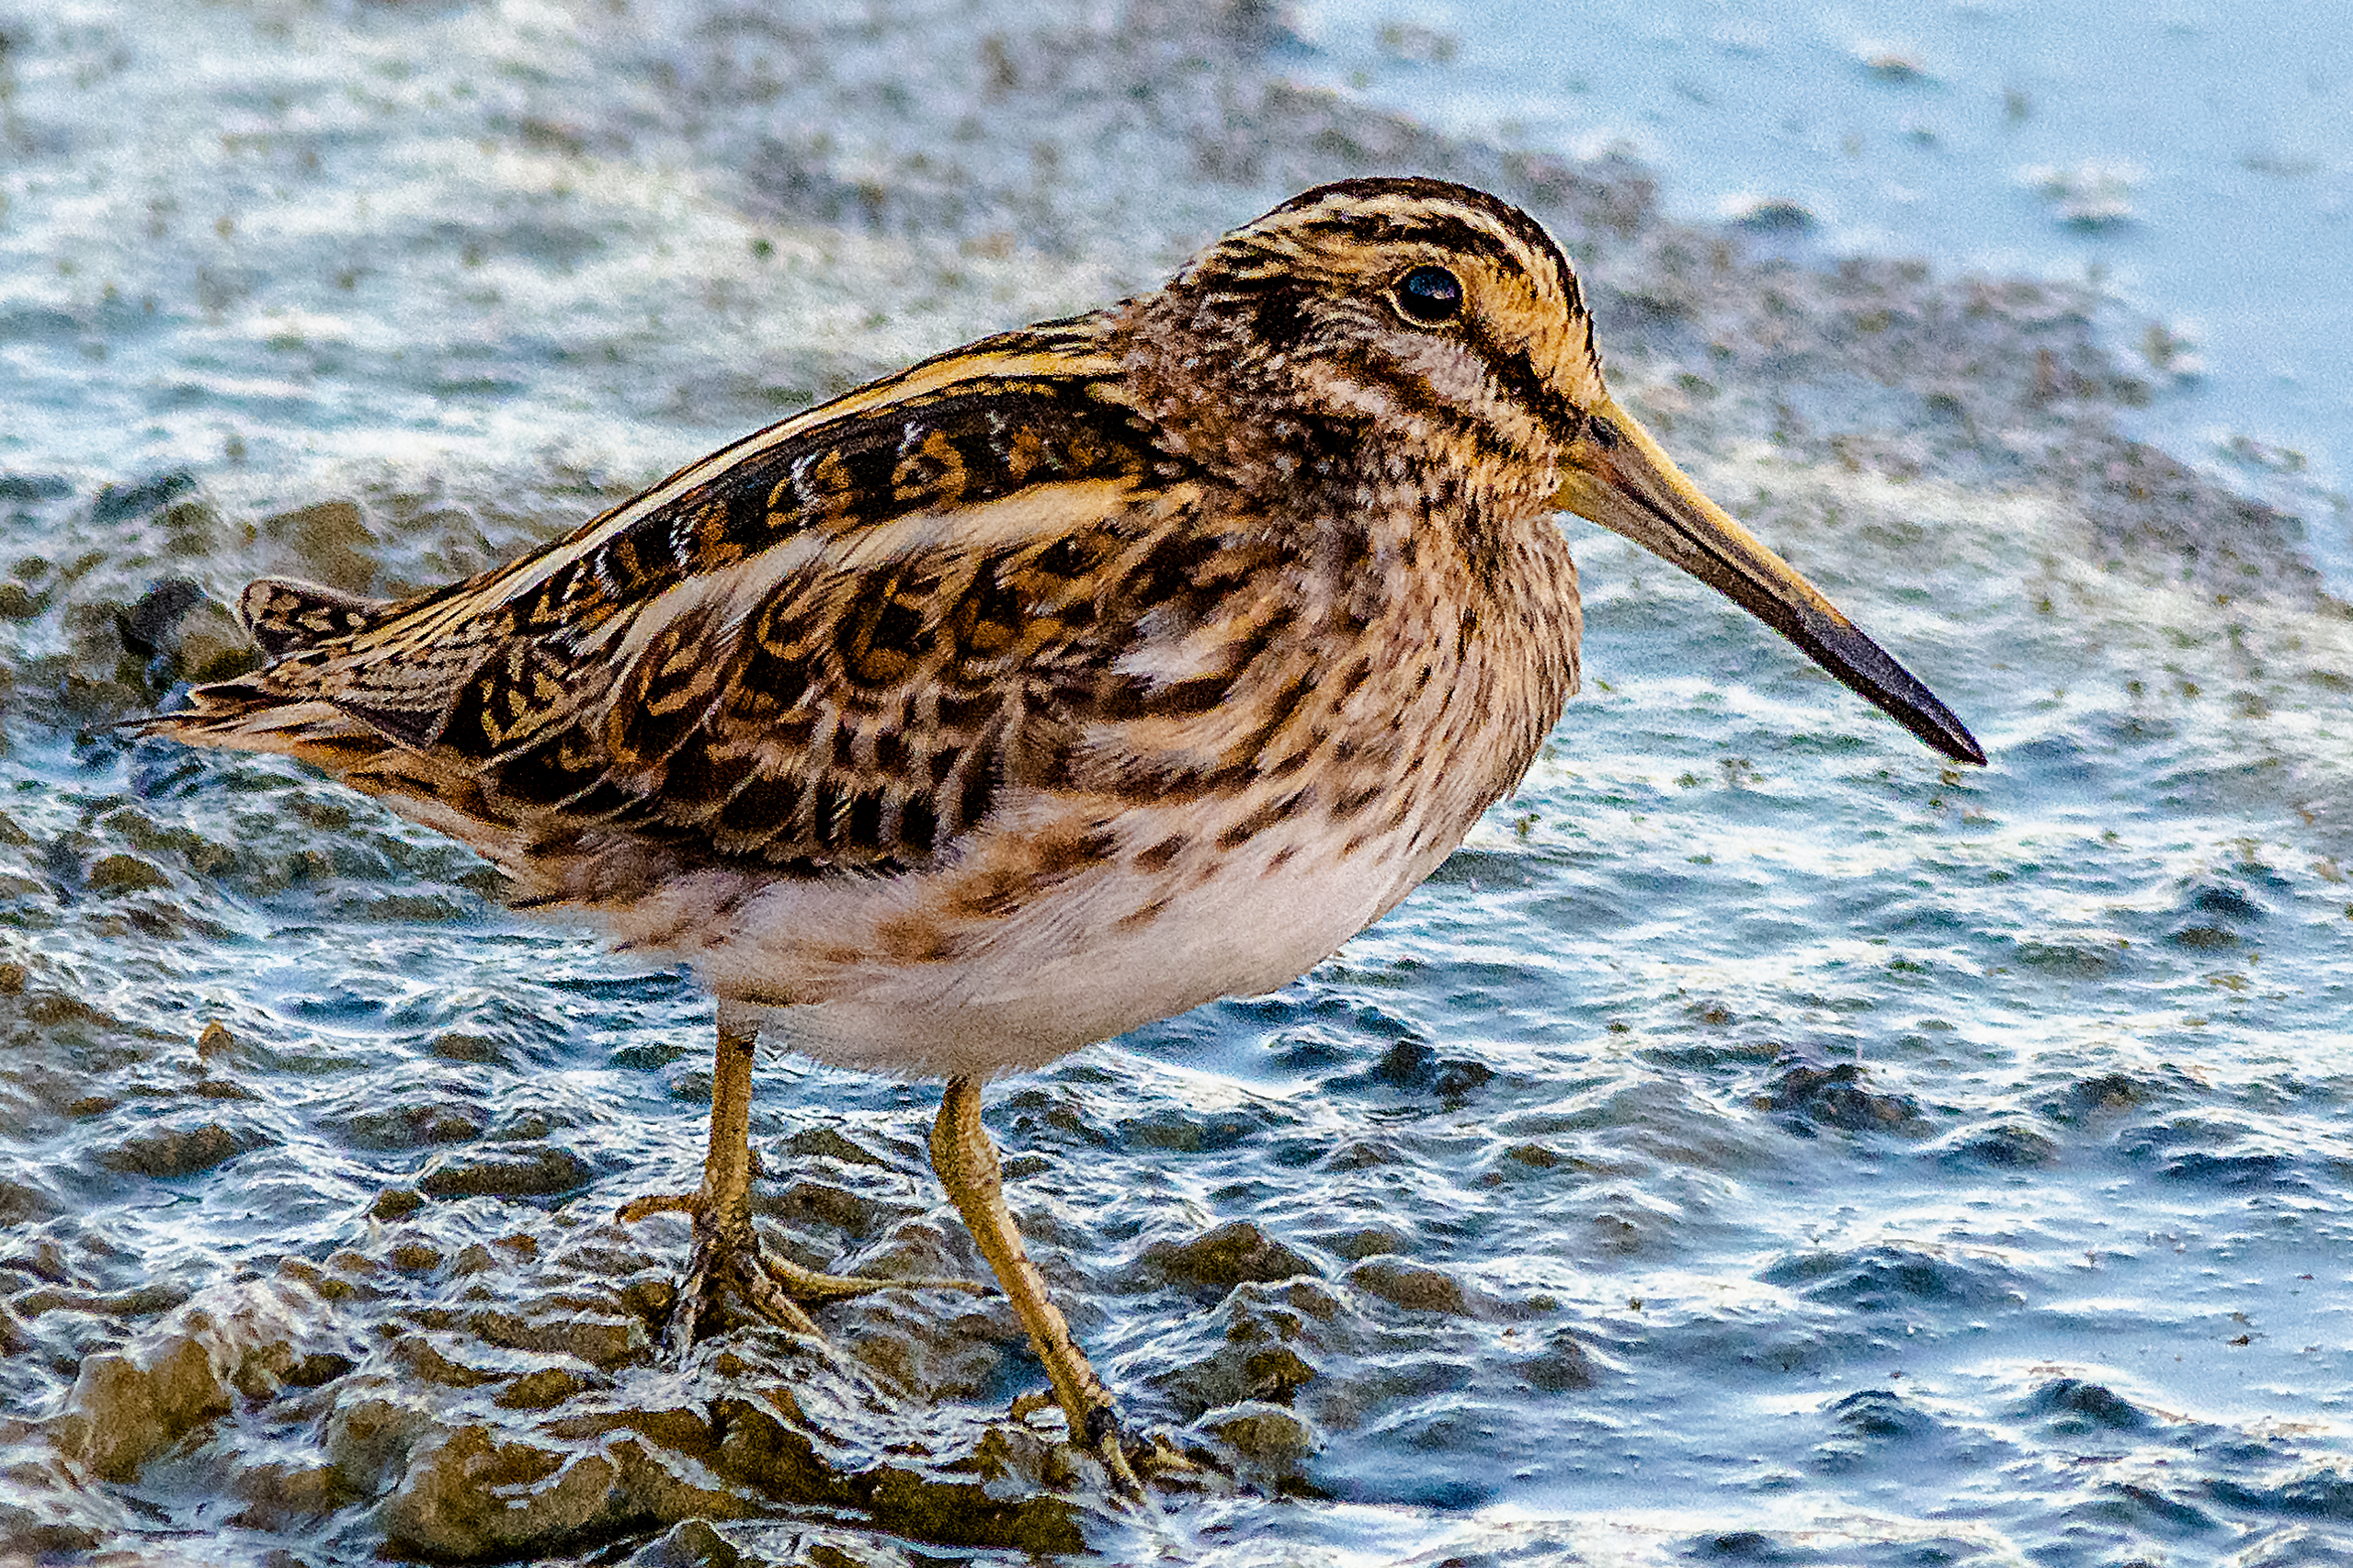
\includegraphics[width=0.8\linewidth, height=10cm, keepaspectratio]{Billeder/Dyr/Fugle/Vadefugle/enkelt_bekkasin.png}
\end{minipage}
}%
\end{columns}
\end{frame}
\begin{frame}{%
\begin{minipage}[t]{0.85\textwidth}
Skovsneppe
\end{minipage}%
\hfill
\begin{minipage}[t]{0.1\textwidth}
\raggedleft

\includegraphics[width=0.5cm, height=0.5cm, keepaspectratio]{Billeder/Ikoner/star.png}%
\hspace{0.2em}%

\includegraphics[width=0.5cm, height=0.5cm, keepaspectratio]{Billeder/Ikoner/star.png}
\end{minipage}%
}
\vspace{0.25em}
\begin{columns}[T]
% --- Venstre kolonne: Tekst ---
\column{0.55\textwidth}
\setlength{\parskip}{0.5em}
\small
\RaggedRight\textbf{\textit{Scolopax rusticola}} – Buttet og kraftig vadefugl med langt næb. Fineste jagttrofæ i Danmark\par 

\textbf{Udseende:} \\
\quad – Stort hoved med brede tværstriber på issen. Store øjne. Spraglet fjerdragt med brun, lysere og mørkere partier  \par

\textbf{Levesteder:} \\
\quad – Lever som eneste vadefugl i skove og læhegn

\textbf{Føde:} \\
\quad – Insekter, orme og snegle \par

\textbf{Udbredelse:} \\
\quad – Hele Danmark \par

\textbf{Træk/standfugl} \\
\quad – Begge \par

% --- Højre kolonne: Kun ét billede (Hannen) ---
\column{0.40\textwidth}
\centering
\fbox{%
\begin{minipage}{\linewidth}
\centering
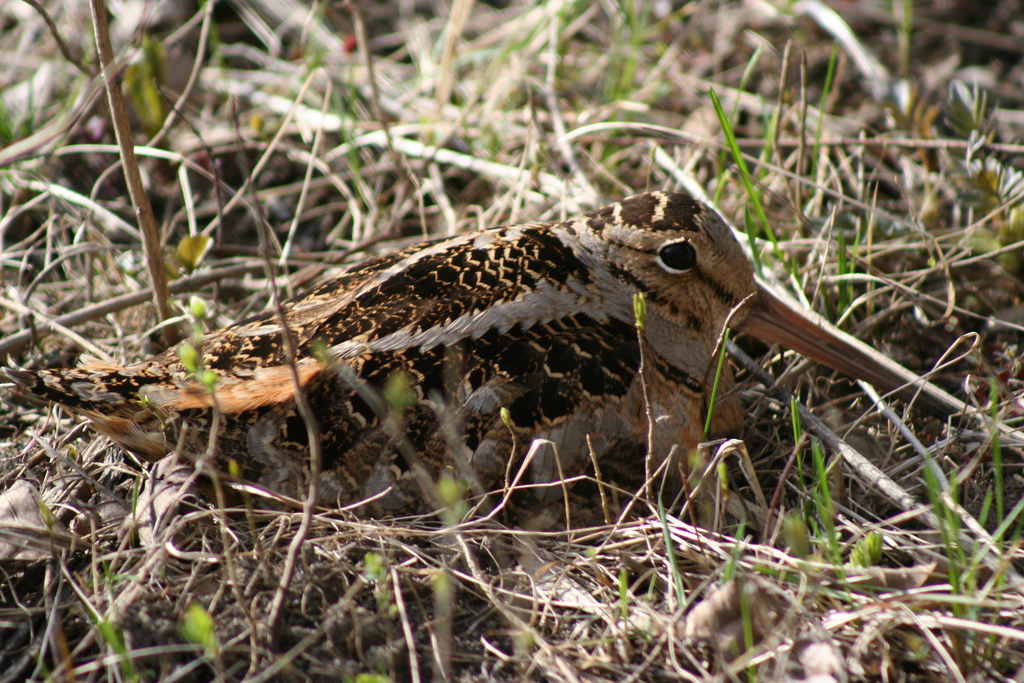
\includegraphics[width=0.8\linewidth, height=6.5cm, keepaspectratio]{Billeder/Dyr/Fugle/Vadefugle/skovsneppe.jpg}%
\end{minipage}
}%
\end{columns}
\end{frame}

\section{Repetition Teori 1-2}

\begin{frame}
  \vspace{3em}
  \begin{center}
    {\LARGE \textbf{Repetition: Teori 1-2 (Kahoot)}}
  \end{center}
\end{frame}

\section{Våbenhåndtering}

\begin{frame}
  \vspace{3em}
  \begin{center}
    {\LARGE \textbf{Våbenhåndtering}}
  \end{center}
\end{frame}



\begin{frame}{Våbenhåndtering – trin for trin}
  \vspace{0.3em} % Mindsket plads
  \begin{columns}[T]
    % --- Venstre kolonne: Opstart + Forhindring (Originalt indhold) ---
    \column{0.48\textwidth}
    \setlength{\parskip}{0.28em} % Mindsket afstand mellem afsnit
    \footnotesize
    \RaggedRight

    \textbf{-- Opstart --} \\
    1. Fødder i skudretning – fri for mennesker. \\
    2. Forskæfte med \textit{modsatte hånd} af skulderen du vil lægge geværet til. \\
    3. Åbn geværet lodret med topnøgle. \\
    4. Kig igennem – \textit{tomt og rent}. \\
    5. Før gennem vandret (knækket). \\
    6. Isæt patroner. \\
    7. Luk i \textbf{45°} – hør \textit{klik}. \\
    8. Før op til \textit{semi-klar}. \\
    9. \textit{Fingre væk} fra aftrækker/sikring. \par

    \vspace{0.3em} % Mindsket plads
    \textbf{-- Forhindring --} \\
    10. Før geværet ned gennem vandret. \\
    11. Åbn – patroner \textit{i lommen}. \\
    12. Forcer med \textit{knækket gevær}. \\
    13. Efterse løbene. \\
    14. Isæt patroner igen. \\
    15. Før op gennem vandret. \par

    % --- Højre kolonne: Skudafgivelse (Originalt indhold) ---
    \column{0.48\textwidth}
    \setlength{\parskip}{0.28em} % Mindsket afstand mellem afsnit
    \footnotesize
    \RaggedRight

    \textbf{-- Skudafgivelse --} \\
    16. Geværet lades \\
    17. Op til \textit{semi-klar}. \\
    18. Kolbe mod bryst – nær armhule. Min 30° \\
    19. Meld: \textbf{„KLAR!“} \\
    20. Afsikring \textit{frem}. \\
    21. Affyr 1–2 skud. \\
    22. Ned til bryst. \\
    23. Sikring \textit{tilbage}. \\
    24. Ned gennem vandret. \\
    25. Åbn – fjern afskudte. \\
    26. Gentag \textbf{4 gange}. \\
    27. Aflever \textit{alle patroner}. \par

  \end{columns}
\end{frame}

%\section{Fasanfugle (vildtkending og biologi)}

% ========== TITEL: FASANFUGLE ==========
\begin{frame}
  \vspace{1.5em}
  \begin{center}
    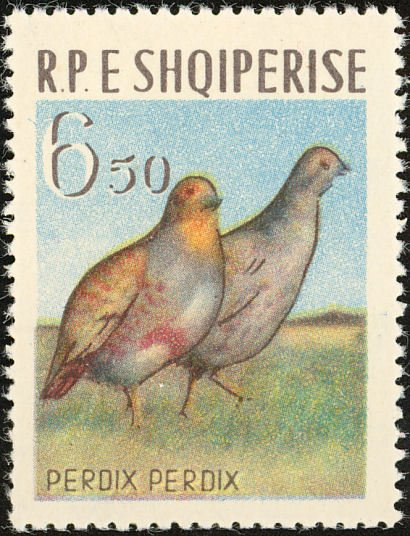
\includegraphics[width=12cm, height=4cm, keepaspectratio]{Billeder/Dyr/Fugle/Fasanfugle/fasanfugle.jpeg}\\[1.2em]
    {\LARGE \textbf{Fasanfugle}}
    \vspace{1em}
    \\ Artsbestemmelse og vildtbiologi
    \\[0.9em]
    {\tiny\color{gray}
    CC BY 4.0 – kan frit anvendes, også kommercielt. Rettighederne må ikke skærpes.\\[0.05em]
    Udviklet af Aleksander Sønder, OSJAGTTEGN.DK}
  \end{center}
\end{frame}

% ========== FASAN ==========
\begin{frame}{%
  \begin{minipage}[c]{0.30\textwidth}
    Fasan
  \end{minipage}%
  \hfill
  \begin{minipage}[c]{0.45\textwidth}
    \footnotesize
    \textbf{Jagttid:} 1.\ oktober -- 31.\ januar
  \end{minipage}%
  \hfill
  \begin{minipage}[c]{0.15\textwidth}
    \noindent\raggedleft
    
\includegraphics[width=0.5cm, height=0.5cm, keepaspectratio]{Billeder/Ikoner/star.png}%
    \hspace{0.2em}%
    
\includegraphics[width=0.5cm, height=0.5cm, keepaspectratio]{Billeder/Ikoner/star.png}%
    \hspace{0.2em}%
    
\includegraphics[width=0.5cm, height=0.5cm, keepaspectratio]{Billeder/Ikoner/star.png}
  \end{minipage}%
}
  \vspace{0.25em}
  \begin{columns}[T]
    % --- Venstre kolonne: Tekst ---
    \column{0.45\textwidth}
    \setlength{\parskip}{0.5em}
    \tiny
    \RaggedRight
    \textbf{\textit{Phasianus colchicus}} – stor hønsefugl med lang hale \par
    \textbf{Udseende:}\\
    \quad – Kok: Kobberrød krop, grønt hoved, røde kindpletter, ofte hvid halsring \\
    \quad – Høne: Brunspraglet, mere camoufleret, kortere hale \par
    \textbf{Levesteder:} Marker, læhegn, småskove og moser. \par
    \textbf{Føde:} Frø, korn, bær, insekter og snegle. \par
    \textbf{Udbredelse:} Hele Danmark. \par
    \textbf{Træk/standfugl:} Standfugl \par
    \textbf{Forplantning:}\\
    \quad – \textbf{Yngleforhold:} Yngler i hele Danmark \\
    \quad – \textbf{Kønsmoden:} Ca. 1 år \\
    \quad – \textbf{Mono/polygam:} Polygam \\
    \quad – \textbf{Bestandsomsætning:} Hurtig \\
    \quad – \textbf{Kuld:} 8–15 æg
    % --- Højre kolonne: To billeder ---
    \column{0.52\textwidth}
    \centering
    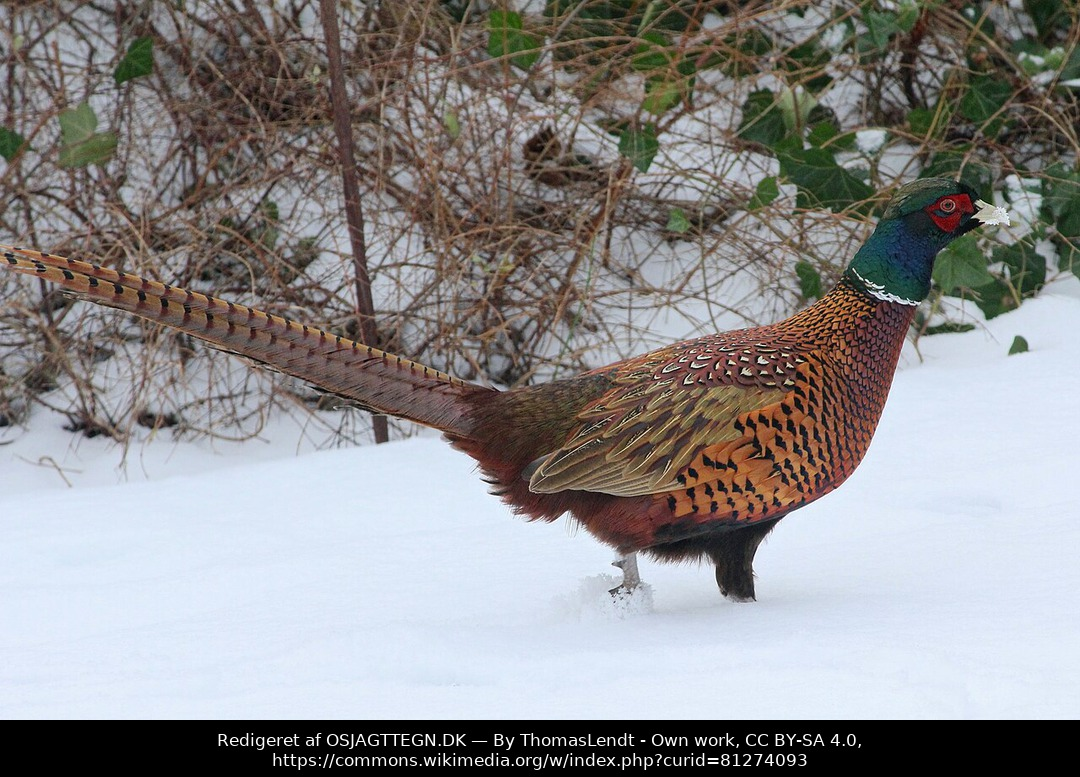
\includegraphics[width=0.92\linewidth, height=3cm, keepaspectratio]{Billeder/Dyr/Fugle/Fasanfugle/Fasan/fasan-male-01.jpg}\\[0.45em]
    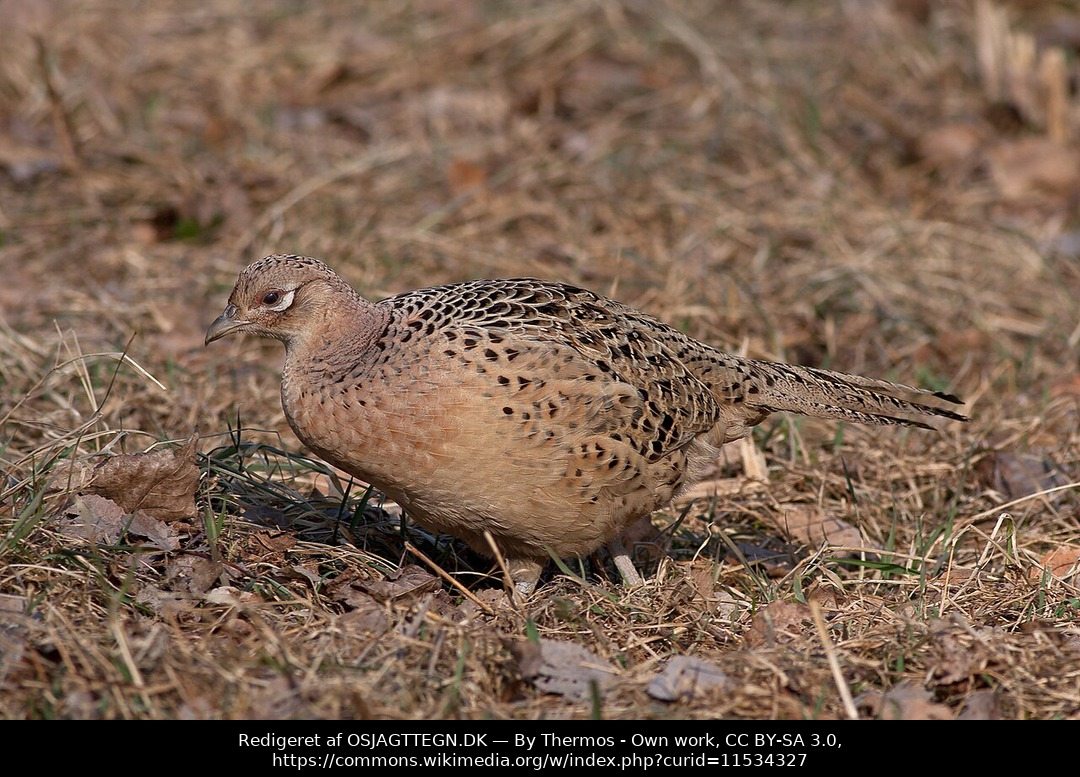
\includegraphics[width=0.92\linewidth, height=3cm, keepaspectratio]{Billeder/Dyr/Fugle/Fasanfugle/Fasan/fasan-female-01.jpg}\\[0.25em]
    \footnotesize Kok øverst, høne nederst
  \end{columns}
\end{frame}
% ========== AGERHØNE ==========
\begin{frame}{%
  \begin{minipage}[c]{0.30\textwidth}
    Agerhøne
  \end{minipage}%
  \hfill
  \begin{minipage}[c]{0.45\textwidth}
    \footnotesize
    \textbf{Jagttid:} 16.\ september -- 31.\ oktober*
  \end{minipage}%
  \hfill
  \begin{minipage}[c]{0.15\textwidth}
    \noindent\raggedleft
    
\includegraphics[width=0.5cm, height=0.5cm, keepaspectratio]{Billeder/Ikoner/star.png}%
    \hspace{0.2em}%
    
\includegraphics[width=0.5cm, height=0.5cm, keepaspectratio]{Billeder/Ikoner/star.png}%
    \hspace{0.2em}%
    
\includegraphics[width=0.5cm, height=0.5cm, keepaspectratio]{Billeder/Ikoner/star.png}
  \end{minipage}%
}
  \vspace{0.25em}
  \begin{columns}[T]
    % --- Venstre kolonne: Tekst ---
    \column{0.45\textwidth}
    \setlength{\parskip}{0.45em}
    \tiny
    \RaggedRight
    \textbf{\textit{Perdix perdix}} – lille, buttet hønsefugl med kort hale \par
    \textbf{Udseende:}\\
    \quad – Gråbrun med orangebrunt ansigt og rødbrun hale \\
    \quad – Han har typisk en større mørk hesteskoformet plet på bugen \par
    \textbf{Levesteder:} Åbent agerland med marker, læhegn, skel og enge. \par
    \textbf{Føde:} Ukrudtsfrø, korn og grønt. Kyllinger lever først af insekter. \par
    \textbf{Udbredelse:} Hele Danmark, men i tilbagegang. \par
    \textbf{Træk/standfugl:} Standfugl \par
    \textbf{Forplantning:}\\
    \quad – \textbf{Yngleforhold:} Yngler i hele Danmark \\
    \quad – \textbf{Kønsmoden:} Ca. 1 år \\
    \quad – \textbf{Mono/polygam:} Monogam \\
    \quad – \textbf{Bestandsomsætning:} Hurtig \\
    \quad – \textbf{Kuld:} 10–20 æg \par
    \textbf{*Bemærk:} Lokale jagttider, især vest for Storebælt.
    % --- Højre kolonne: Ét billede ---
    \column{0.52\textwidth}
    \centering
    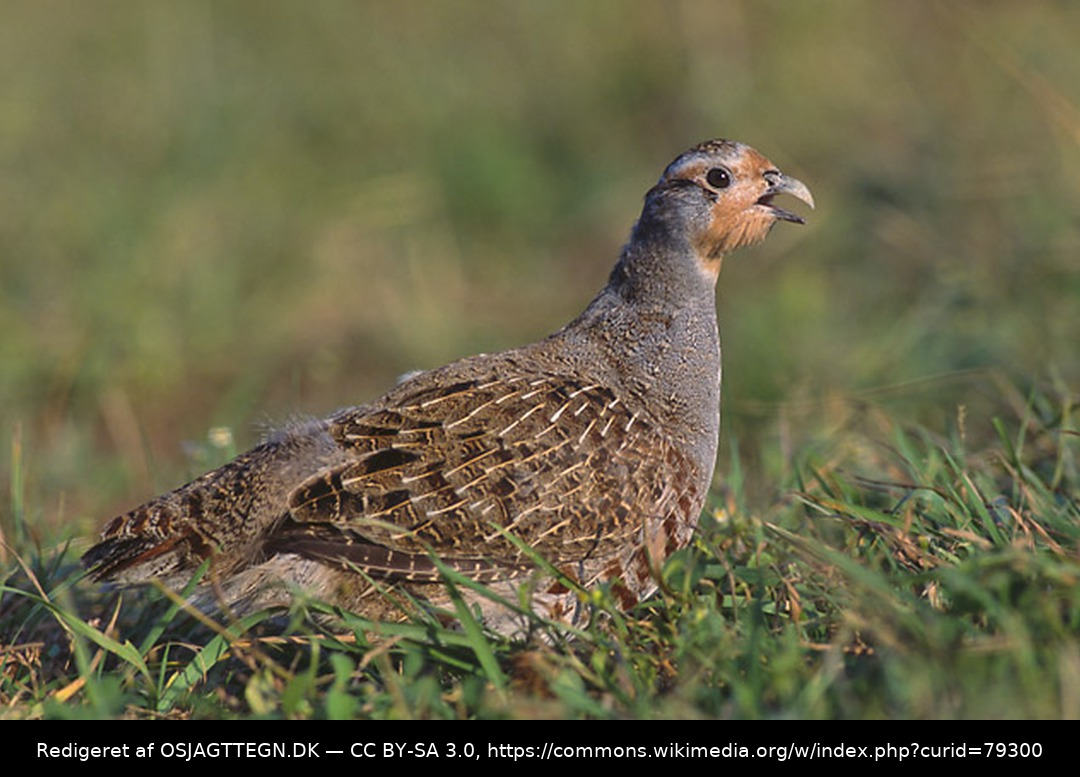
\includegraphics[width=\linewidth, height=7.2cm, keepaspectratio]{Billeder/Dyr/Fugle/Fasanfugle/Agerhøne/agerhoene-01.jpg}
  \end{columns}
\end{frame}

%\section{Udsætning af vildt}

\begin{frame}
  \vspace{3em}
  \begin{center}
    {\LARGE \textbf{Udsætning af vildt}
    }
    \\
    \vspace{1em}
    Bekendtgørelse om udsætning af vildt, jagtmåder og jagtredskaber
    \\
    \vspace{1em}
    BEK nr 1652 af 19/12/2017, Kapitel 6
  \end{center}
\end{frame}

\begin{frame}{Generelt vedrørende udsætning af vildt}

\textbf{Hovedregel:} \\
Vildt må \textbf{ikke} udsættes i naturen uden tilladelse fra myndigheden.

\textbf{Undtagelse – kun disse tre arter må udsættes uden tilladelse:}
\begin{itemize}
    \item \textbf{Fasan} (Phasianus colchicus): 1. april – 31. august
    \item \textbf{Agerhøne} (Perdix perdix): 1. april – 15. august
    \item \textbf{Gråand} (Anas platyrhynchos): 1. april – 31. juli (i ferske vande)
\end{itemize}

\textbf{Vigtige fælleskrav for alle tre arter:}
\begin{itemize}
    \item \textbf{Alle} udsætninger skal indberettes digitalt senest 1 uge efter
    \item Udsætning af \textbf{mere end 100 fugle i alt} (fasan + agerhøne + gråand) kræver gennemført \textbf{godkendt kursus}
    \item Fravigelse fra basisreglerne (f.eks. højere tæthed end 1/ha for fasan/agerhøne) kræver \textbf{biotopplan}
\end{itemize}

\textbf{Alle andre vildtarter:} \\
Kræver særskilt tilladelse – udsætning er generelt forbudt.

\end{frame}




\begin{frame}{Udsætning af fasaner}

\begin{columns}[T] % T = top-aligned

\begin{column}{0.48\textwidth}
\textbf{Regler ved udsætning af fasaner:}
\begin{itemize}
    \item Kan udsættes 1. april til 31. august 
    \item Under 100ha max 100 fugle
    \item Over 100ha 1 fugl pr ha
    \item Biotopplan implementeret op til 7 fugle pr ha
    \item 5 årig biotopplan 2 år inde implementeret op til 12 fugle pr ha
    \item Afvigelser fra 1 fugle pr ha afhænger af pointsystem
    \item Alle udsætninger skal indberettes senest 1 uge efter udsætningen
\end{itemize}
\end{column}

\begin{column}{0.3\textwidth}
    % Vælg én af disse – de ser godt ud i præsentation
    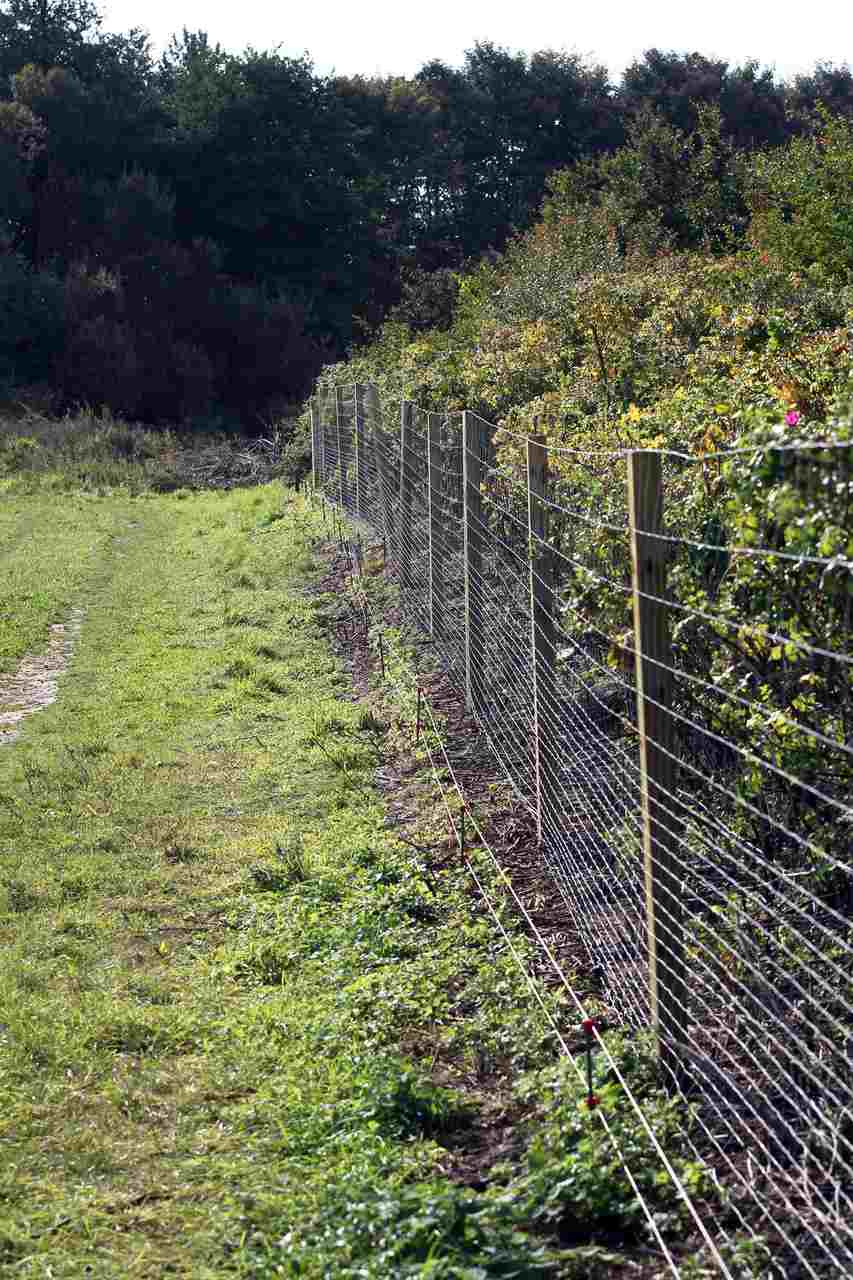
\includegraphics[width=\textwidth]{Billeder/Vildtforvaltning/udsætning/fasanvoilere.jpg}
    % Eller brug et af de gode eksempler:
    % \includegraphics[width=\textwidth]{vegetationsstriber_midtmark_ex.jpg}
\end{column}

\end{columns}

\end{frame}



\begin{frame}{Udsætning af agerhøns }

\begin{columns}[T] % T = top-aligned

\begin{column}{0.48\textwidth}
\textbf{Regler ved udsætning af agerhøns:}
\begin{itemize}
    \item Kan udsættes 1. april til 15. august
    \item Under 100 ha max 100 fugle
    \item Over 100 ha 1 fugl pr. ha
    \item Biotopplan implementeret op til 4 agerhøns pr. ha)
    \item 5-årig biotopplan 2 år inde implementeret op til max 4 agerhøns pr. ha
    \item Afvigelser fra 1 fugl pr. ha afhænger af pointsystem
    \item Alle udsætninger skal indberettes senest 1 uge efter udsætningen
\end{itemize}
\end{column}

\begin{column}{0.4\textwidth}
    % Godt billede af agerhøne eller biotop med agerhøns
    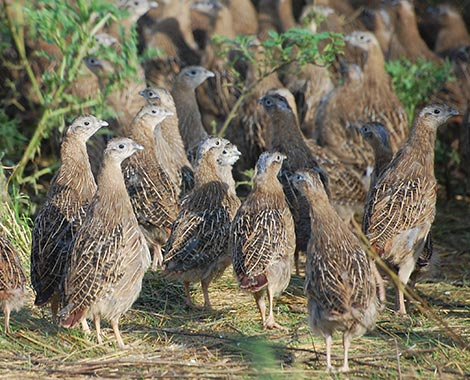
\includegraphics[width=\textwidth]{Billeder/Vildtforvaltning/udsætning/agerhøns.jpg}
    % Alternativer: agerhøne_i_mark.jpg eller vegetationsstriber_agerhoene.jpg
\end{column}

\end{columns}

\end{frame}




\begin{frame}{Udsætning af gråænder}

\begin{columns}[T] % T = top-aligned

\begin{column}{0.48\textwidth}
\textbf{Regler i ferske vande:}
\begin{itemize}
    \item Kan udsættes 1. april til 31. juli
    \item 1 ælling pr. 150 m² åben vandflade
    \item Eller 1 voksen and pr. 300 m² åben vandflade
    \item Ingen generel ha-begrænsning som ved fasan/agerhøne
    \item Ingen biotopplan-krav for højere antal
    \item Alle udsætninger skal indberettes senest 1 uge efter udsætningen
    \item Over 100 fugle (samlet med fasan/agerhøne) kræver godkendt kursus
\end{itemize}
\end{column}

\begin{column}{0.3\textwidth}
    % Vælg én af disse – de ser godt ud i præsentation
    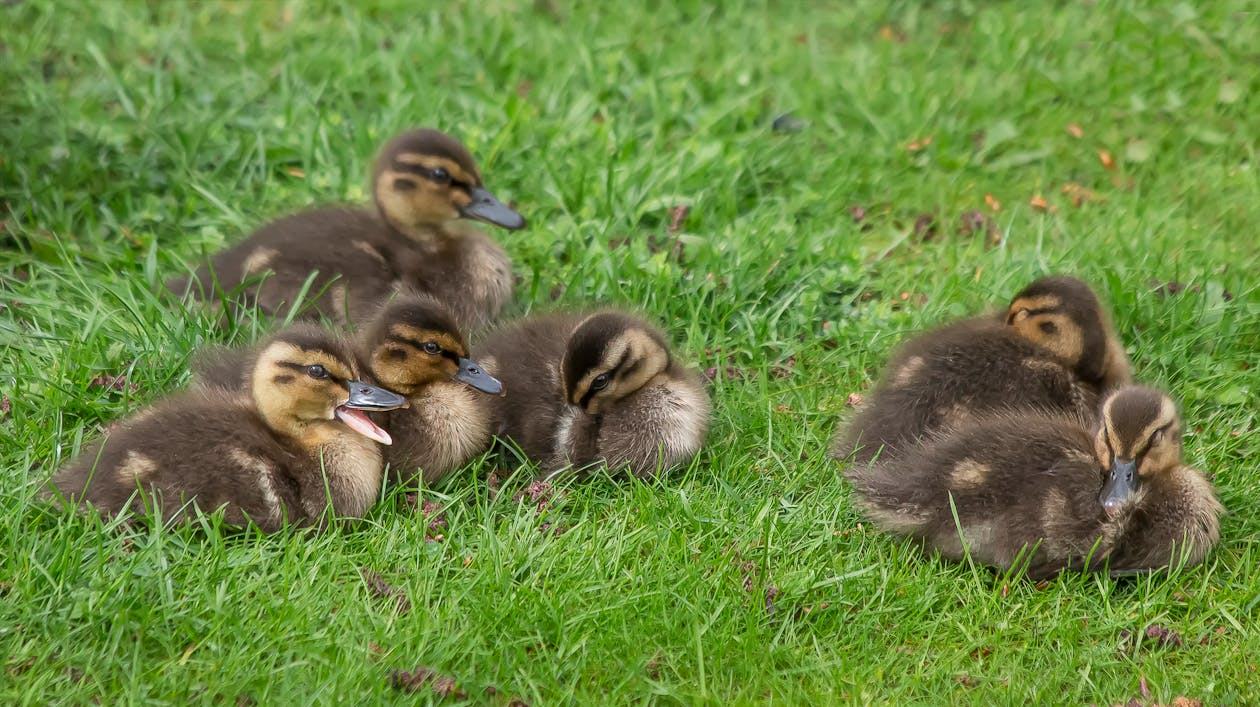
\includegraphics[width=\textwidth]{Billeder/Vildtforvaltning/udsætning/gråandeællinger.jpeg}
    % Eller brug et af de gode eksempler:
    % \includegraphics[width=\textwidth]{vegetationsstriber_midtmark_ex.jpg}
\end{column}

\end{columns}

\end{frame}

%\section{Vildtforvaltning}

\begin{frame}
  \vspace{3em}
  \begin{center}
    {\LARGE \textbf{Vildtforvaltning: biotopplantiltag}
    }
    \\
    \vspace{1em}
    Bekendtgørelse om udsætning af vildt, jagtmåder og jagtredskaber
    \\
    \vspace{1em}
    BEK nr 1652 af 19/12/2017, Bilag 2
  \end{center}
\end{frame}

\begin{frame}{Biotopplaner ved udsætning af agerhøns \& fasaner}
  \begin{itemize}
    \item \textbf{Formål}: Etablere/forbedre biotoper for vildt (fugle \& pattedyr) + naturlig flora/fauna
    \item \textbf{Gennemført}: Tiltag skal være udført senest 1. juni i ansøgningsåret
    \item \textbf{Biotopplan-ejendom}: Sammenhængende arealer med samme ejer/bruger (ekskl. søer >1 ha)
    \item \textbf{Biotopplan-areal}: Non-food lavskov, dyrkede/udyrkede landbrugsarealer + udyrkede bræmmer
    \item \textbf{Krav}: Gælder kun landbrugsmæssigt dyrkede arealer
    \item Uden biotopplan: Maks. 1 fugl/ha (eller 100 stk. på <100 ha)
    \item Med biotopplan: Op til 7 fugl/ha (max 4 agerhøns/ha) ved min. point
  \end{itemize}
\end{frame}

\begin{frame}{Udsætningsgrænser \& pointkrav}
  \begin{itemize}
    \item \textbf{1-årig plan}: Min. 100 point → op til 7 fugl/ha
    \item \textbf{3-årig plan}: Min. 85 point → op til 7 fugl/ha
    \item \textbf{5-årig plan} (for 8–12 fugl/ha): Ekstra point udover basis
      \begin{itemize}
        \item 110 point → max 8 fugl/ha
        \item 120 point → max 9 fugl/ha
        \item 130 point → max 10 fugl/ha
        \item 140 point → max 11 fugl/ha
        \item 150 point → max 12 fugl/ha (max 4 agerhøns/ha)
      \end{itemize}
    \item \textbf{Særlige vilkår for 8–12/ha}: Skal have 5-årig plan + erfaring (forudgående 2 år med biotopplan)
    \item Ejendomme uden landbrugsarealer eller <22 ha dyrket areal: Op til 7 fugl/ha uden plan på ikke-dyrket del
    \item \textbf{Indberetning}: Senest 1 uge efter udsætning til Miljøstyrelsens digitale system
  \end{itemize}
\end{frame}

\begin{frame}{Krav til biotopplanens indhold \& opretholdelse}
  \begin{itemize}
    \item \textbf{Min. indhold}:
      \begin{itemize}
        \item Udpegning af arealer + tiltag på opdateret markkort (max 1:10.000)
        \item Beskrivelse + størrelse af hvert tiltag
        \item Om rævefælder forventes brugt
        \item Ansvarlig persons navn/adresse/tlf.
      \end{itemize}
    \item \textbf{Anmeldelse}: Til Miljøstyrelsen senest 1. maj (digitalt)
    \item \textbf{Opretholdelse}: Tiltag holdes i planperioden (1/3/5 år) – undtaget lærkepletter, randzoner mv. (til høst/20. feb.)
    \item \textbf{Placering}: Forbedrer naturindhold, korridorer til hegn/skove/vandløb, hensyn til mikroklima
    \item \textbf{Målrettet}: Min. 4 arter/artsgrupper (mindst 2 ikke-jagtbare)
    \item \textbf{Kontrol}: 5–10 \% stikprøver årligt af Naturstyrelsen
    \item \textbf{Kursuskrav}: Ved >100 fugl total (fasan/agerhøns/gråænder) – godkendt kursus kræves
  \end{itemize}
\end{frame}

\begin{frame}{Uddrag af pointsystemet}
  \centering
  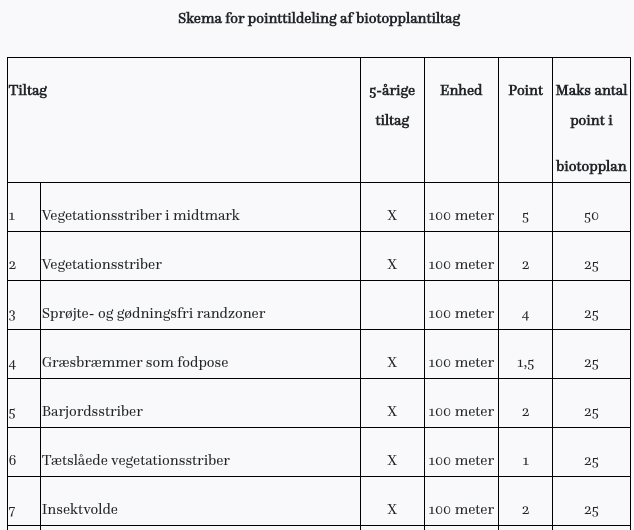
\includegraphics[width=\textwidth, height=0.8\textheight, keepaspectratio]{Billeder/Vildtforvaltning/biotopplantiltag/pointsystem.png}
\end{frame}


\begin{frame}
  \vspace{3em}
  \begin{center}
    {\LARGE \textbf{17 tiltag}
    }
    \\
    \vspace{1em}
    Jagttegnsaspiranter skal kende til 17 af pointgivende tiltag
    \\
    \vspace{1em}
    
  \end{center}
\end{frame}

% 17 tiltag til forbedringer for markvildtet

\begin{frame}{Vegetationsstriber i midtmark}

\small

\begin{columns}[T]

\begin{column}{0.58\textwidth}

\textbf{Regler ved vegetationsstriber i marken:}

\begin{itemize}[]
\item Uddyrket eller vildt- og bivenlig vegetation
\item Må ikke isås med kulturgræsser
\item Min. 3 m bred
\item Min. 40 m til kanten af det dyrkede areal
\item Må ikke gødskes eller sprøjtes
\item Ved 3- og 5-årige biotopplaner: maks. 30\% omlægges årligt
\end{itemize}

\vspace{0.4em}

\textbf{Gavner arter:}

\footnotesize
Agerhøne, fasan, hare, rådyr, dådyr, sanglærke, vibe, gul vipstjert, 
rødrygget tornskade, gulspurv, vilde bier, humlebier, 
dagsommerfugle, rovbiller, græshopper, markmus, pindsvin, lækat, flagermus, 
musvåge, tårnfalk

\end{column}

\begin{column}{0.40\textwidth}
\centering
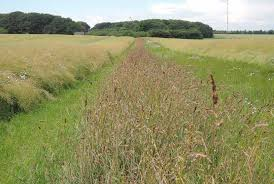
\includegraphics[width=\textwidth]{Billeder/Vildtforvaltning/biotopplantiltag/vildtstribemidtmark.jpeg}
\end{column}

\end{columns}

\end{frame}

\begin{frame}{Vegetationsstriber}

\small

\begin{columns}[T]

\begin{column}{0.58\textwidth}

\textbf{Regler ved vegetationsstriber:}

\begin{itemize}[]
\item Etableres langs søer, vandløb  og lign.
\item Uddyrket eller vildt- og bivenlig vegetation
\item Må ikke isås med kulturgræsser
\item Min. 3 m bred
\item Må ikke gødskes eller sprøjtes
\item Ved 3- og 5-årige biotopplaner: maks. 30\% af tiltaget omlægges årligt
\end{itemize}

\vspace{0.4em}

\textbf{Gavner arter:}

\footnotesize
Agerhøne, fasan, hare, rådyr, dådyr, sanglærke, vibe, gul vipstjert, 
rødrygget tornskade, gulspurv, vilde bier, humlebier, dagsommerfugle, 
rovbiller, græshopper, markmus, pindsvin, lækat, flagermus, musvåge, tårnfalk

\end{column}

\begin{column}{0.40\textwidth}
\centering
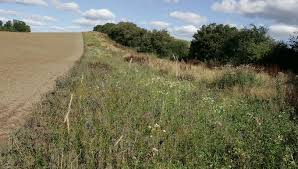
\includegraphics[width=\textwidth]{Billeder/Vildtforvaltning/biotopplantiltag/vegetationsstribe.jpeg}
\end{column}

\end{columns}

\end{frame}




\begin{frame}{Sprøjte- og gødningsfrie randzoner}

\small

\begin{columns}[T]

\begin{column}{0.58\textwidth}

\textbf{Regler ved sprøjte- og gødningsfrie randzoner:}

\begin{itemize}[]
\item Følger produktionsarealer og skal være minimum 6 m brede
\item Kan ikke placeres samme sted som andre biotopplantiltag
\item Skal opretholdes i biotopplanen fra såning og frem til høst
\end{itemize}

\vspace{0.4em}

\textbf{Gavner arter:}

\footnotesize
Vilde bier, humlebier, dagsommerfugle, svirrefluer, rovbiller, græshopper, 
gul vipstjert, sanglærke, agerhøne, vibe, rødrygget tornskade, gulspurv, 
markpiber, markmus, pindsvin, lækat, flagermus, musvåge, tårnfalk

\end{column}

\begin{column}{0.40\textwidth}
\centering
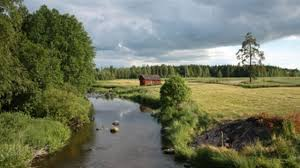
\includegraphics[width=\textwidth]{Billeder/Vildtforvaltning/biotopplantiltag/randzone.jpeg}
\end{column}

\end{columns}

\end{frame}

\begin{frame}{Græsbræmmer som fodpose}

\small

\begin{columns}[T]

\begin{column}{0.58\textwidth}

\textbf{Regler for græsbræmmer som fodpose:}

\begin{itemize}[]
\item Fodpose langs søer, vandløb, kystlinjer, vådområder, levende hegn, skovbryn, markskel og lign.
\item Består primært af græsser og urtevegetation
\item Min. 2 m bred
\item Min. 50\% soleksponeret
\item Må ikke gødskes eller sprøjtes
\end{itemize}

\vspace{0.4em}

\textbf{Gavner arter:}

\footnotesize
Agerhøne, fasan, hare, rådyr, sanglærke, vibe, gul vipstjert, rødrygget tornskade, 
gulspurv, markpiber, vilde bier, humlebier, dagsommerfugle, rovbiller, græshopper, 
overvintrende insekter, markmus, pindsvin, lækat, flagermus, musvåge, tårnfalk

\end{column}

\begin{column}{0.40\textwidth}
\centering
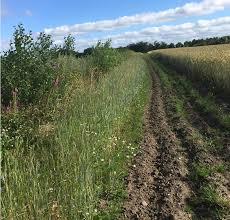
\includegraphics[width=\textwidth]{Billeder/Vildtforvaltning/biotopplantiltag/græsbræmme.jpeg}
\end{column}

\end{columns}

\end{frame}

\begin{frame}{Barjordsstriber}

\small

\begin{columns}[T]

\begin{column}{0.58\textwidth}

\textbf{Regler for barjordsstriber:}

\begin{itemize}[]
\item Udlægges langs søer, vandløb, kystlinjer, vådområder, levende hegn, skovbryn, markskel, diger, fortidsminder, beplantning, vegetationsstriber og naturarealer
\item Min. 1 m bred
\item Min. 50\% soleksponeret
\item Plantedække max. 20\% over 100 m strækning
\end{itemize}

\vspace{0.4em}

\textbf{Gavner arter:}

\footnotesize
Vibe, agerhøne, sanglærke, gul vipstjert, 
rødrygget tornskade, gulspurv, vilde bier, humlebier, dagsommerfugle, 
rovbiller, græshopper, markmus, pindsvin, lækat, musvåge, tårnfalk

\end{column}

\begin{column}{0.40\textwidth}
\centering
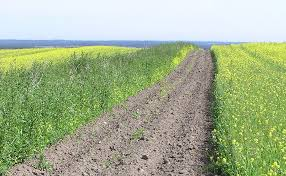
\includegraphics[width=\textwidth]{Billeder/Vildtforvaltning/biotopplantiltag/barjordsstribe.jpeg}
\end{column}

\end{columns}

\end{frame}

\begin{frame}{Tætslåede vegetationsstriber}

\small

\begin{columns}[T]

\begin{column}{0.58\textwidth}

\textbf{Regler for tætslåede vegetationsstriber:}

\begin{itemize}[]
\item Holdes kort ved hyppig slåning
\item Må ikke kunne indbyde til redeskjul
\item Min. 2 m brede
\item Max. 6 m brede
\item Min. 20 m mellem striberne
\end{itemize}

\vspace{0.4em}

\textbf{Gavner arter:}

\footnotesize
Vibe, sanglærke, markpiber, finke, agerhøne, gul vipstjert, 
rødrygget tornskade, gulspurv, vilde bier, humlebier, dagsommerfugle, 
svirrefluer, rovbiller, græshopper, markmus, pindsvin, musvåge, tårnfalk

\end{column}

\begin{column}{0.40\textwidth}
\centering
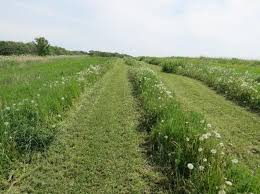
\includegraphics[width=\textwidth]{Billeder/Vildtforvaltning/biotopplantiltag/slået_vegetationsstribe.jpeg}
\end{column}

\end{columns}

\end{frame}

\begin{frame}{Insektvolde}

\small

\begin{columns}[T]

\begin{column}{0.58\textwidth}

\textbf{Regler for insektvolde:}

\begin{itemize}[]
\item Tilsås med tuegræsser
\item Min. 20 m mellem voldene
\item Min. 50\% soleksponeret
\item Skal kunne etableres og fjernes med landbrugsmaskiner
\item Min. 1 m bred
\end{itemize}

\vspace{0.4em}

\textbf{Gavner arter:}

\footnotesize
Vilde bier, humlebier, solitære bier, dagsommerfugle, svirrefluer, rovfugle, 
græshopper, overvintrende insekter, gul vipstjert, rødrygget tornskade, 
pirol, svaler, flagermus, pindsvin, lækat, musvåge, tårnfalk

\end{column}

\begin{column}{0.40\textwidth}
\centering
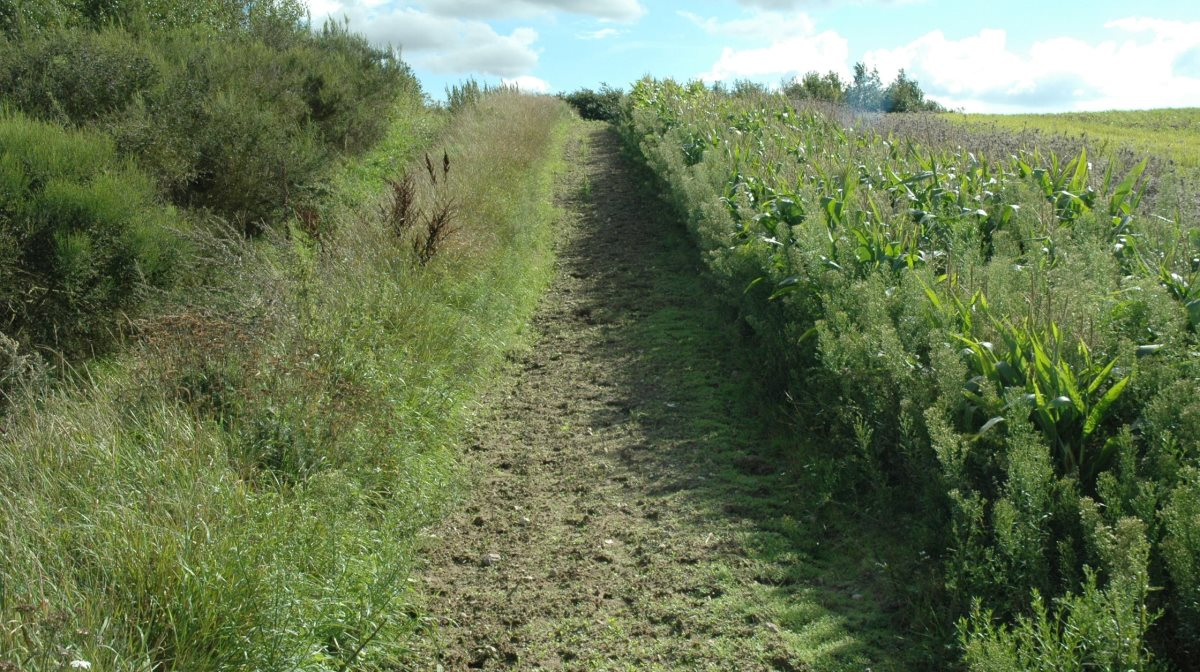
\includegraphics[width=\textwidth]{Billeder/Vildtforvaltning/biotopplantiltag/insektvold.jpg}
\end{column}

\end{columns}

\end{frame}

\begin{frame}{Kyllingestriber}

\small

\begin{columns}[T]

\begin{column}{0.58\textwidth}

\textbf{Regler for kyllingestriber:}

\begin{itemize}[]
\item Tilsås med 30\% udsædsmængde (synlig reduktion ift. tilstødende areal)
\item Minimum 3 m brede
\item Skal kombineres med tiltaget "sprøjte- og gødningsfri randzone"
\end{itemize}

\vspace{0.4em}

\textbf{Gavner arter:}

\footnotesize
Agerhøne, fasan, sanglærke, vibe, markpiber, gul vipstjert, 
rødrygget tornskade, gulspurv, agerpistol, vilde bier, humlebier, 
dagsommerfugle, rovbiller, græshopper, markmus, pindsvin, musvåge, tårnfalk

\end{column}

\begin{column}{0.40\textwidth}
\centering
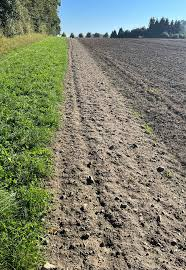
\includegraphics[width=\textwidth]{Billeder/Vildtforvaltning/biotopplantiltag/kyllingestriber.jpeg}
\end{column}

\end{columns}

\end{frame}

\begin{frame}{Lærkepletter}

\small

\begin{columns}[T]

\begin{column}{0.58\textwidth}

\textbf{Regler for lærkepletter:}

\begin{itemize}[]
\item Mindst 16 m²
\item Min. 2 per hektar
\item Mindst 40 m til kanten af marken
\item Må ikke gødskes eller sprøjtes
\end{itemize}

\vspace{0.4em}

\textbf{Gavner arter:}

\footnotesize
Sanglærke, bomlærke, vibe, agerhøne, markpiber, agerpistol, gul vipstjert, 
rødrygget tornskade, gulspurv, vilde bier, humlebier, dagsommerfugle, 
rovbiller, græshopper, musvåge, tårnfalk

\end{column}

\begin{column}{0.40\textwidth}
\centering
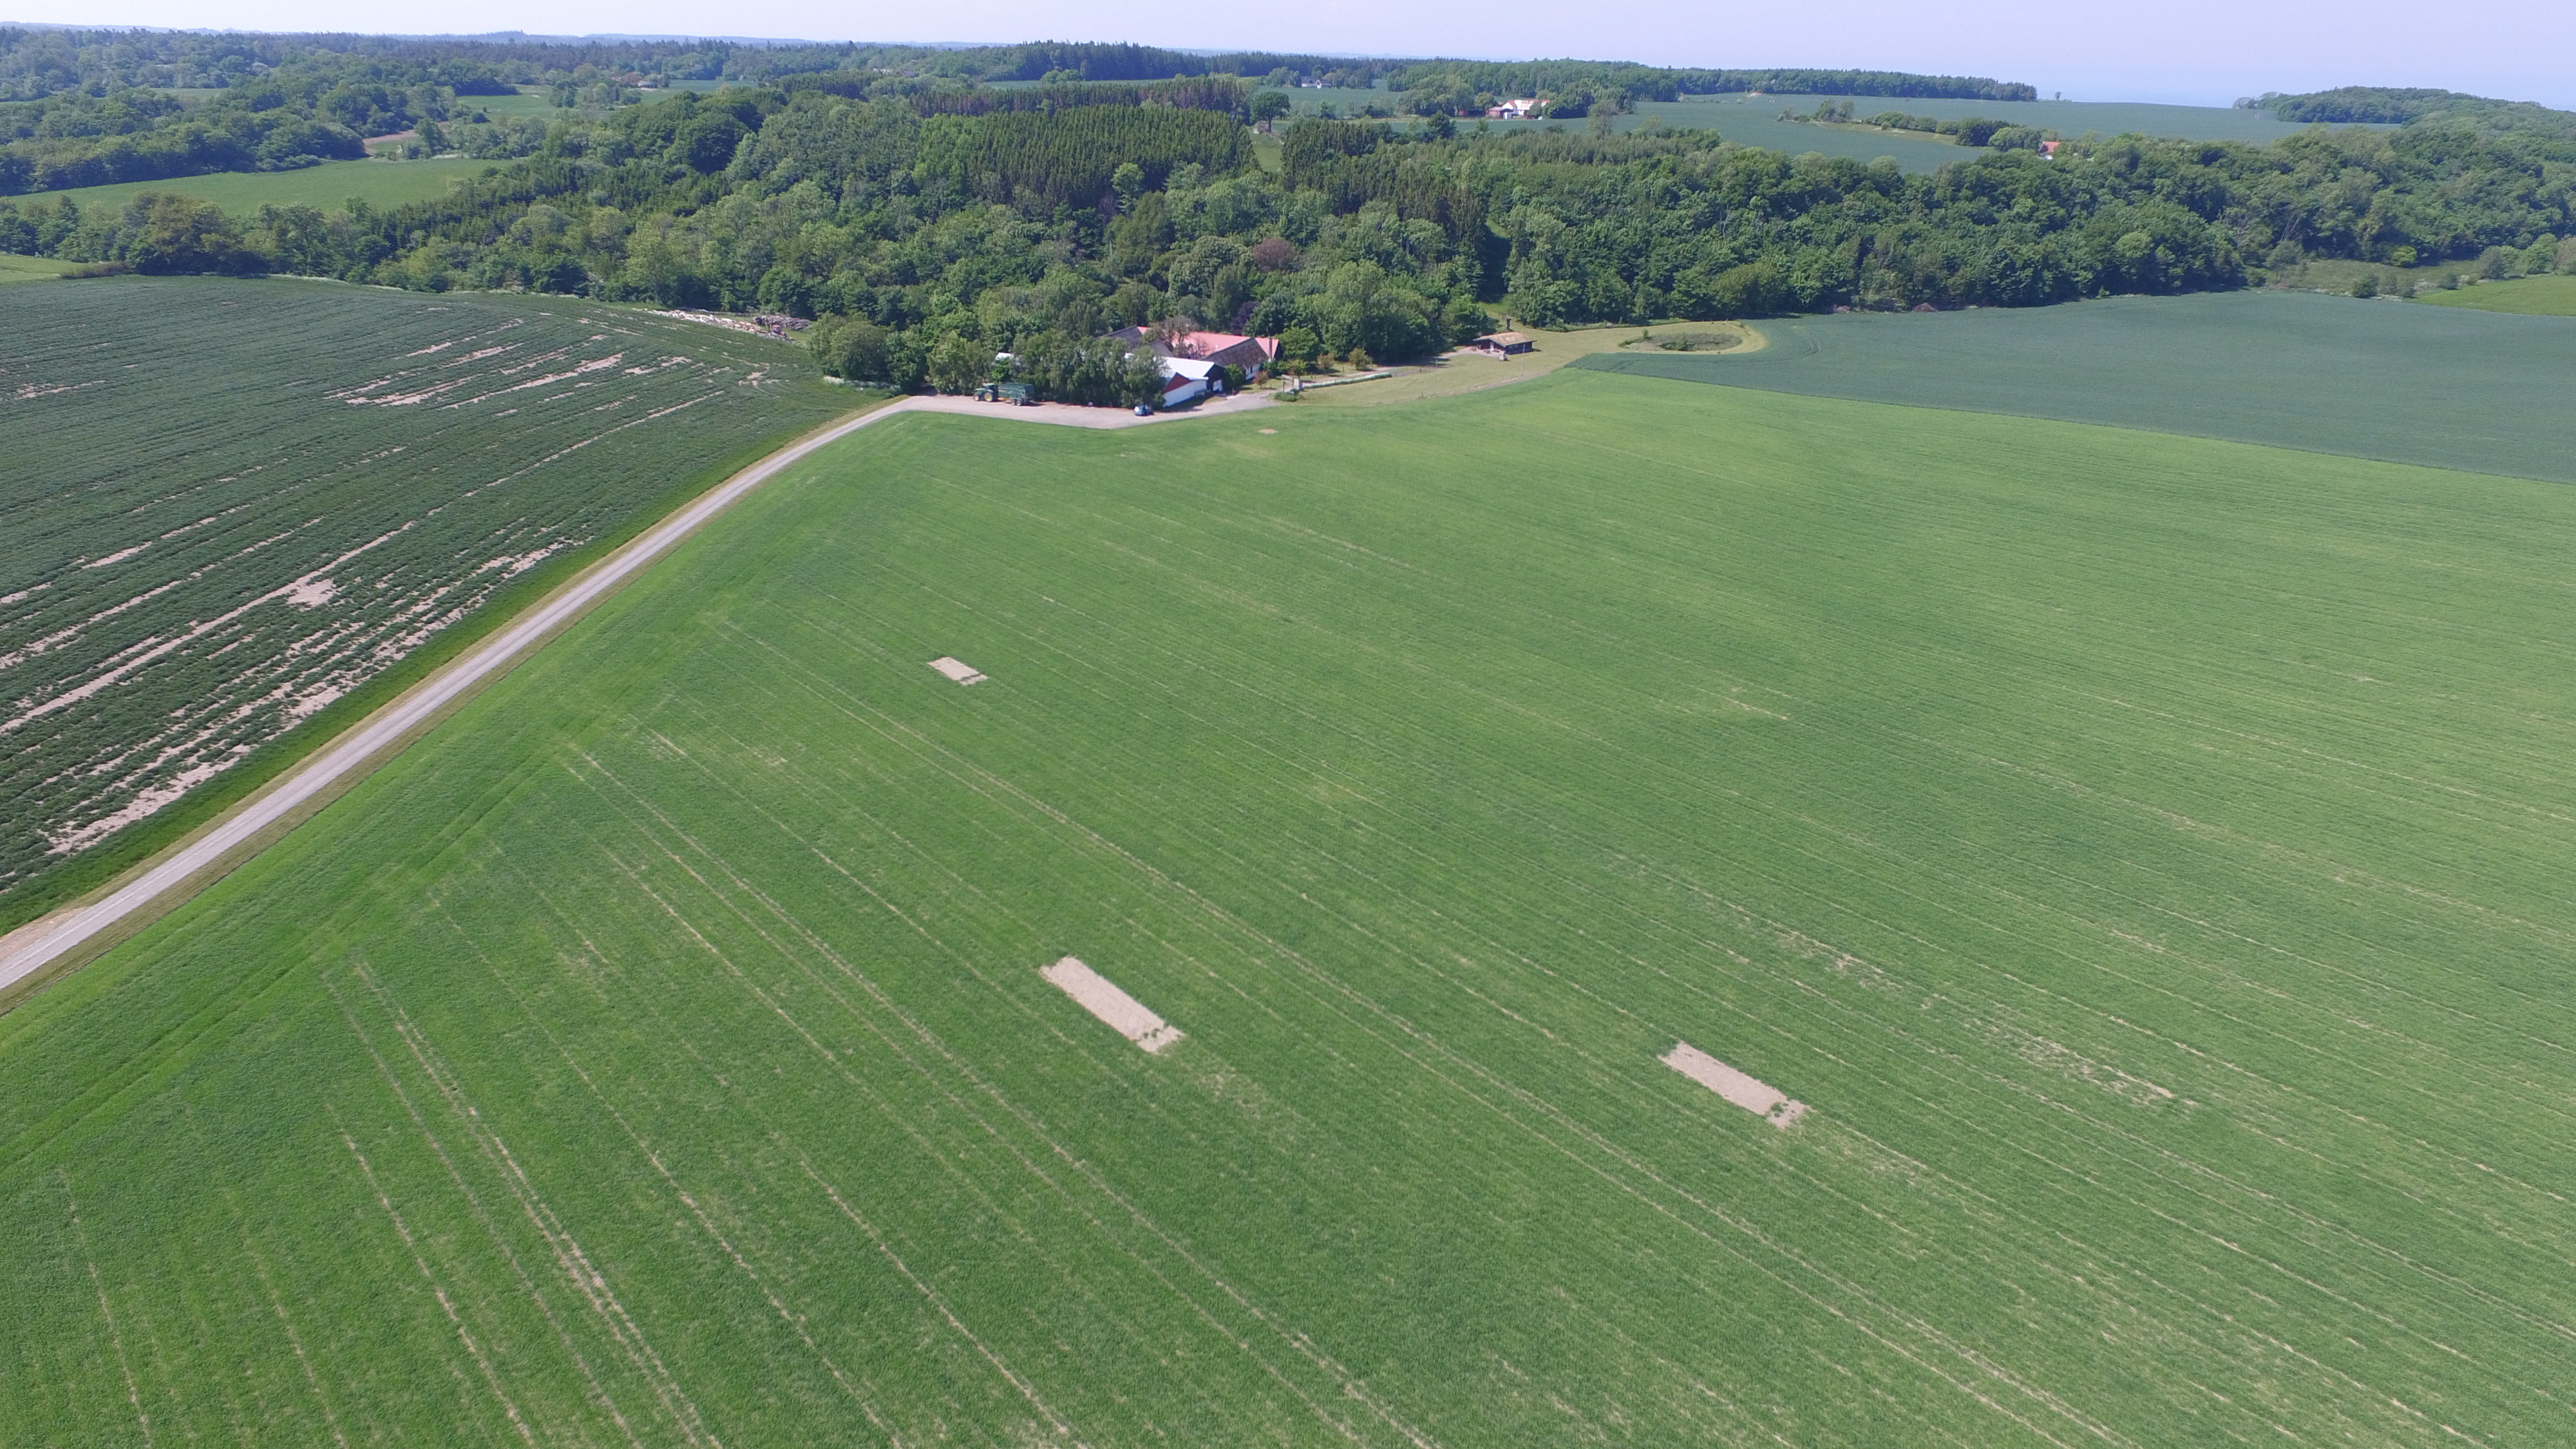
\includegraphics[width=\textwidth]{Billeder/Vildtforvaltning/biotopplantiltag/lærkepletter.jpeg}
\end{column}

\end{columns}

\end{frame}

\begin{frame}{Vibelavninger}

\small

\begin{columns}[T]

\begin{column}{0.58\textwidth}

\textbf{Regler for vibelavninger:}

\begin{itemize}[]
\item Min. 16 m²
\item Min. 1 pr. ha
\item Min. 40 m til markkant
\item Må ikke gødskes eller sprøjtes
\end{itemize}

\vspace{0.4em}

\textbf{Gavner arter:}

\footnotesize
Vibe, sanglærke, agerhøne, dobbeltbekkasin, engpiber, gul vipstjert, 
rødrygget tornskade, gulspurv, markpiber, vilde bier, humlebier, 
dagsommerfugle, rovbiller, græshopper, pindsvin, musvåge, tårnfalk

\end{column}

\begin{column}{0.40\textwidth}
\centering
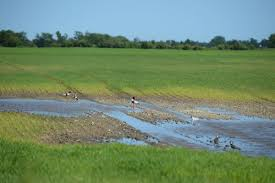
\includegraphics[width=\textwidth]{Billeder/Vildtforvaltning/biotopplantiltag/vibelavninger.jpeg}
\end{column}

\end{columns}

\end{frame}

\begin{frame}{Lysåben vegetation / arronderinger}

\small

\begin{columns}[T]

\begin{column}{0.58\textwidth}

\textbf{Regler for lysåben vegetation / arronderinger:}

\begin{itemize}[]
\item \textbf{Arrondering}: Fx afrunding af hjørner i marken
\item Kan bestå af: græsarealer, naturlig vegetation (udyrket areal) og/eller vildtstriber
\item \textbf{Græsarealer}: Primært græs, plejet kort via afgræsning eller høslet
\item \textbf{Vildtstriber}: Tilsået med vildt- og bivenlige plantearter
\item Tilladte arter: Alle ikke-traditionelle afgrøder i renbestand
\end{itemize}

\vspace{0.05em}

\textbf{Gavner arter:}

\footnotesize
Agerhøne, fasan, hare, rådyr, sanglærke, vibe, gul vipstjert, 
rødrygget tornskade, gulspurv, markpiber, vilde bier, humlebier, 
dagsommerfugle, svirrefluer, rovbiller, græshopper, markmus, 
pindsvin, lækat, flagermus, musvåge, tårnfalk

\end{column}

\begin{column}{0.40\textwidth}
\centering
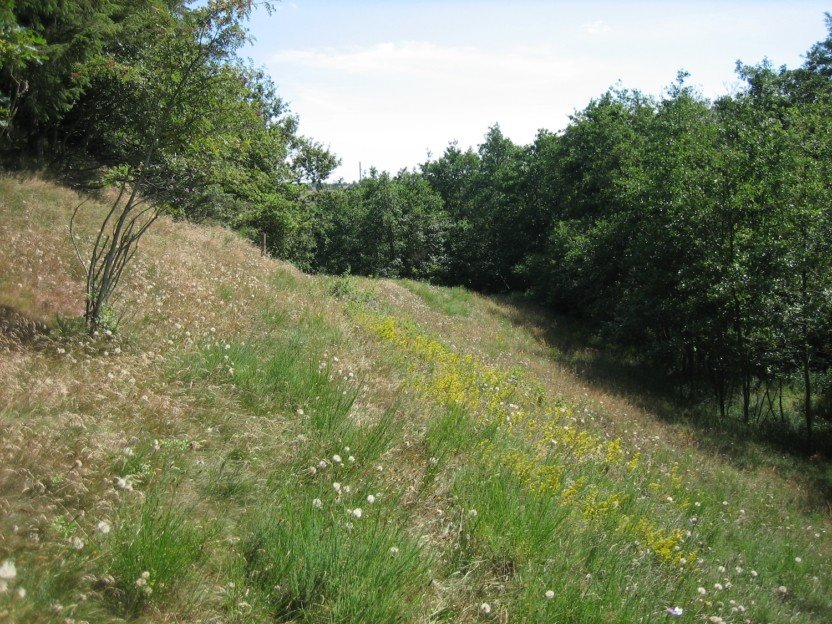
\includegraphics[width=\textwidth]{Billeder/Vildtforvaltning/biotopplantiltag/lysåben.jpg}
\end{column}

\end{columns}

\end{frame}

\begin{frame}{Stubmark og efterafgrøder}

\small

\begin{columns}[T]

\begin{column}{0.58\textwidth}

\textbf{Regler for stubmark og efterafgrøder:}

\begin{itemize}[]
\item Efterafgrøde kan være korsblomstrede afgrøder (f.eks. olieræddike, gul sennep, cikorie) eller græs og kornafgrøder
\item Efterafgrøder skal ligge vinteren over til den 20. februar
\item Min. 1 m bred
\end{itemize}

\vspace{0.4em}

\textbf{Gavner arter:}

\footnotesize
Fasan, hare, rådyr, sanglærke, agerhøne, gul vipstjert, rødrygget tornskade, 
gulspurv, agerspurv, gråspurv, markspurv, vild due, vilde bier, humlebier, 
overvintrende insekter, markmus, pindsvin, musvåge, tårnfalk, rødhals

\end{column}

\begin{column}{0.40\textwidth}
\centering
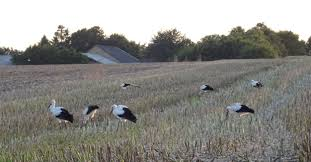
\includegraphics[width=\textwidth]{Billeder/Vildtforvaltning/biotopplantiltag/stubmark.jpeg}
% Bemærk: Jeg ændrede filnavnet til stubmark.jpg – tilpas det til dit faktiske billede
\end{column}

\end{columns}

\end{frame}

\begin{frame}{Etablering af træ- og buskbevoksninger}

\small

\begin{columns}[T]

\begin{column}{0.58\textwidth}

\textbf{Regler for etablering af træ- og buskbevoksninger:}

\begin{itemize}[]
\item Max. 0,5 ha pr. tiltag
\item Min. 50 m mellem tiltag
\end{itemize}

\vspace{0.4em}

\textbf{Gavner arter:}

\footnotesize
Fasan, agerhøne, markhare, rådyr, dådyr, rødrygget tornskade, gul vipstjert, 
pirol, gulspurv, blåmejse, musvit, sortmejse, grønsisken, stillits, 
rødhals, flagermus, pindsvin, lækat, egern, musvåge, spurvehøg, tårnfalk

\end{column}

\begin{column}{0.40\textwidth}
\centering
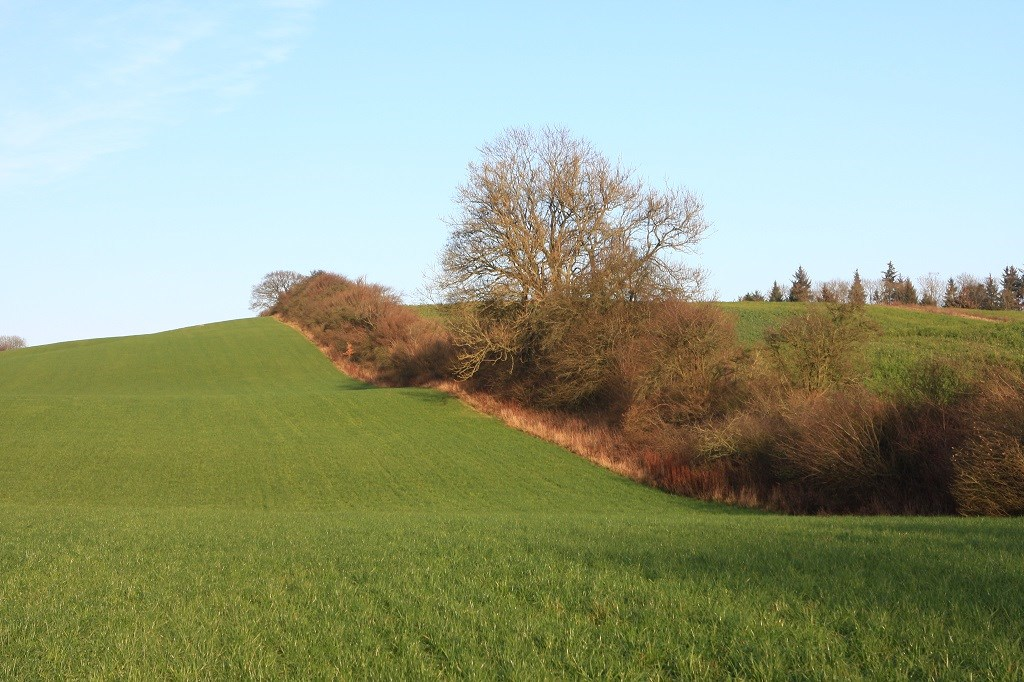
\includegraphics[width=\textwidth]{Billeder/Vildtforvaltning/biotopplantiltag/buskbevoksning.jpg}
\end{column}

\end{columns}

\end{frame}

\begin{frame}{Etablering af levende hegn og linieformede markopdelinger}

\small

\begin{columns}[T]

\begin{column}{0.58\textwidth}

\textbf{Regler for etablering af levende hegn og linieformede markopdelinger:}

\begin{itemize}[]
\item Min. 2 m bred
\item Anlægges langs grøfter, diger, veje mm.
\item Ved mere end tre rækker: lysåbning hver 50. meter
\end{itemize}

\vspace{0.4em}

\textbf{Gavner arter:}

\footnotesize
Fasan, agerhøne, markhare, rådyr, dådyr, rødrygget tornskade, gul vipstjert, 
pirol, gulspurv, blåmejse, musvit, sortmejse, grønsisken, stillits, rødhals, 
nattergal, hærfugl, flagermus, pindsvin, lækat, egern, musvåge, spurvehøg, 
tårnfalk, rørhøg

\end{column}

\begin{column}{0.40\textwidth}
\centering
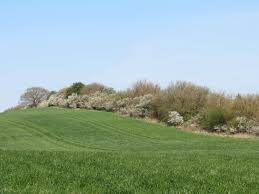
\includegraphics[width=\textwidth]{Billeder/Vildtforvaltning/biotopplantiltag/levendehegn.jpeg}
\end{column}

\end{columns}

\end{frame}

\begin{frame}{Levende hegn og linieformede markopdelinger}

\small

\begin{columns}[T]

\begin{column}{0.58\textwidth}

\textbf{Regler for levende hegn og linieformede markopdelinger:}

\begin{itemize}[]
\item Min. 2 m bred
\item Min. 75\% hjemmehørende arter efter 10 år
\item Skal løbende plejes med beskæring
\item Skal suppleres for at opnå point
\end{itemize}

\vspace{0.4em}

\textbf{Gavner arter:}

\footnotesize
Fasan, agerhøne, markhare, rådyr, dådyr, rødrygget tornskade, gul vipstjert, 
pirol, gulspurv, blåmejse, musvit, sortmejse, grønsisken, stillits, rødhals, 
nattergal, hærfugl, flagermus, pindsvin, lækat, egern, musvåge, spurvehøg, 
tårnfalk, rørhøg

\end{column}

\begin{column}{0.40\textwidth}
\centering
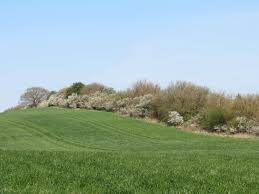
\includegraphics[width=\textwidth]{Billeder/Vildtforvaltning/biotopplantiltag/levendehegn.jpeg}
\end{column}

\end{columns}

\end{frame}

\begin{frame}{Etablering af skov}

\small

\begin{columns}[T]

\begin{column}{0.58\textwidth}

\textbf{Regler for etablering af skov:}

\begin{itemize}[]
\item Opfylder regler for skovrejsning
\item Skal opfylde kravene for tilskud under skovrejsningsordningerne
\item Tiltaget er pointgivende i 5 år fra anlæggelsesåret
\end{itemize}

\vspace{0.4em}

\textbf{Gavner arter:}

\footnotesize
Rådyr, dådyr, ræv, hare, fasan, rødrygget tornskade, gul vipstjert, 
pirol, gulspurv, blåmejse, musvit, sortmejse, grønsisken, stillits, rødhals, 
nattergal, hærfugl, flagermus, pindsvin, lækat, egern, musvåge, spurvehøg, 
tårnfalk, rørhøg, rådyr, kronvildt (senere stadier)

\end{column}

\begin{column}{0.40\textwidth}
\centering
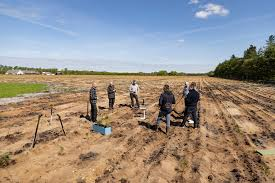
\includegraphics[width=\textwidth]{Billeder/Vildtforvaltning/biotopplantiltag/skovrejsning.jpeg}
\end{column}

\end{columns}

\end{frame}

\begin{frame}{Etablering af søer}

\small

\begin{columns}[T]

\begin{column}{0.58\textwidth}

\textbf{Regler for etablering af søer:}

\begin{itemize}[]
\item Min. 600 m²
\item Minimum 10 m bufferzone
\item Min. 50\% af bufferzonen skal være soleksponeret
\item Pointgivende i 5 år fra anlæggelsestidspunktet
\end{itemize}

\vspace{0.4em}

\textbf{Gavner arter:}

\footnotesize
Vibe, engsnarreskade, dobbeltbekkasin, rødbenet klire, gul vipstjert, 
sanglærke, agerhøne, gråstrubet lappedykker, gråand, krikand, 
padder (frøer, tudser, salamandere), guldsmed, libeller, 
vilde bier (kant), humlebier, markmus, pindsvin, flagermus, 
musvåge, tårnfalk, rørhøg

\end{column}

\begin{column}{0.40\textwidth}
\centering
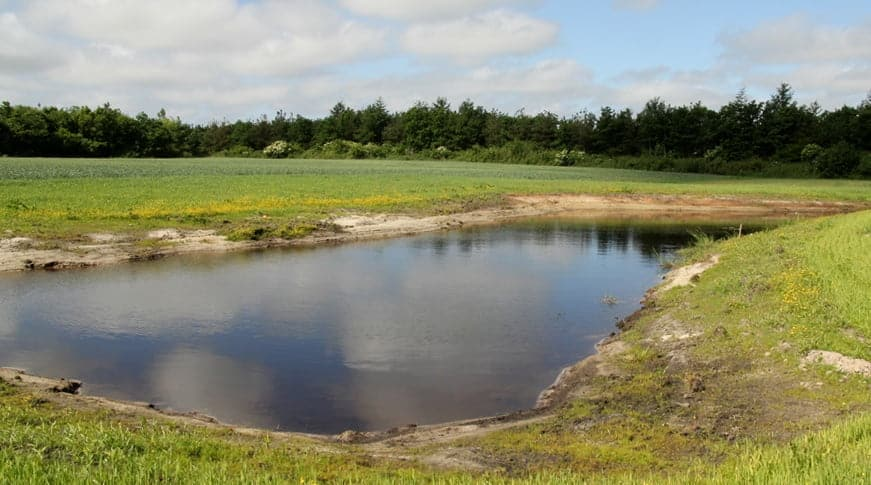
\includegraphics[width=\textwidth]{Billeder/Vildtforvaltning/biotopplantiltag/etableringafsø.jpg}
\end{column}

\end{columns}

\end{frame}

%\section{Æggebekendtgørelsen}

\begin{frame}
  \vspace{3em}
  \begin{center}
    {\LARGE \textbf{"Æggebekendtgørelsen"}
    }
    \\
    \vspace{1em}
    Bekendtgørelse om æg fra vilde fugle og registrering af ægsamlinger
    \\
    \vspace{1em}
    BEK nr 936 af 27/06/2016, §§ 1 og 2
  \end{center}
\end{frame}


\begin{frame}{Bekendtgørelse om æg fra vilde fugle - Omfang (§ 1)}
\vspace{1em}

\small

\raggedright

\begin{itemize}

\itemsep0.6em % Justér afstand mellem bullets

\item Bekendtgørelsen omfatter æg fra vilde fugle, der er naturligt forekommende i den danske natur, samt æg fra arter omfattet af Fuglebeskyttelsesdirektivet (2009/147/EF) og underarter.

\item Gælder også tomme æg samt dele og produkter af æg.

\item Styrelsen for Vand- og Naturforvaltning afgør, om et æg er omfattet, og kan ved tvivl kræve anmeldelse/registrering.

\item Omfatter \textbf{ikke} æg fra landbrugsmæssigt opdræt af visse dyrearter.

\end{itemize}

\end{frame}



\begin{frame}{Bekendtgørelse om æg fra vilde fugle - Forbud og undtagelser (§ 2)}
\vspace{1em}

\small

\raggedright

\begin{itemize}

\itemsep0.6em % Justér afstand mellem bullets

\item Æg fra vilde fugle må \textbf{ikke} indsamles i naturen, opbevares, besiddes, modtages, købes, sælges, overdrages, udlånes, transporteres eller udstilles – medmindre anden lovgivning tillader det.

\item Undtagelser gælder for:
    \begin{itemize}
    \itemsep0.3em
    \item Indsamling af æg fra gråand i kunstige rugepladser
    \item Æg fra ødelagte reder af fasan, gråand eller agerhøne (til opdræt)
    \item Æg fra fasaner indfanget med særlig tilladelse fra styrelsen
    \end{itemize}

\item Den, der besidder æg fra fangenskabsopdrættede fugle af omfattede arter, skal kunne \textbf{godtgøre}, at æggene ikke stammer fra vilde fugle.

\end{itemize}

\end{frame}

%\section{Måger (vildtkending og biologi)}

% ========== TITEL: MÅGEFUGLE ==========
\begin{frame}
  \vspace{1.5em}
  \begin{center}
    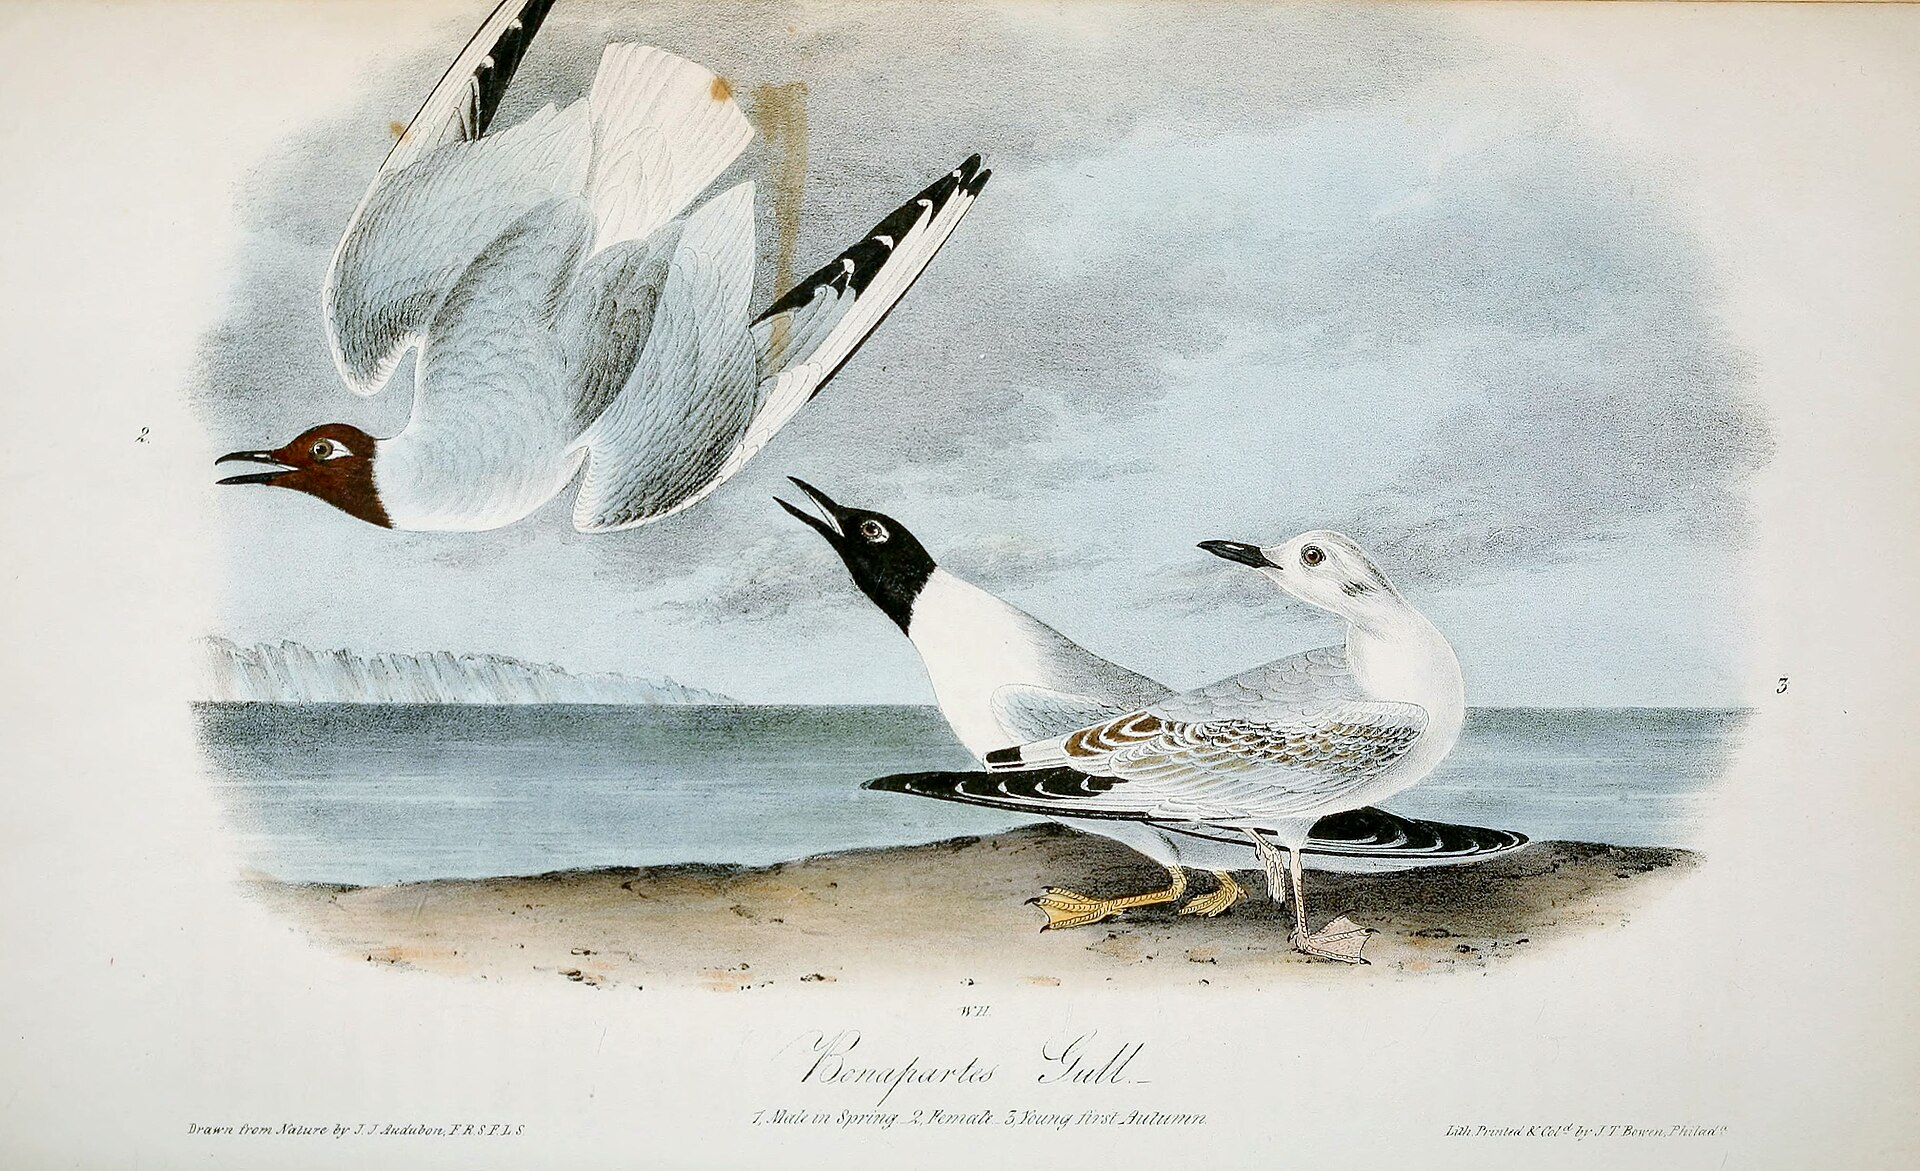
\includegraphics[width=12cm, height=4cm, keepaspectratio]{Billeder/Dyr/Fugle/Mågefugle/maagefugle.jpg}\\[1.2em]
    {\LARGE \textbf{Mågefugle}}\\[0.6em]
   
    Artsbestemmelse \& vildtbiologi\\[0.9em]
    {\tiny\color{gray}
    CC BY 4.0 – kan frit anvendes, også kommercielt. Rettighederne må ikke skærpes.\\[0.05em]
    Udviklet af Aleksander Sønder, OSJAGTTEGN.DK}
  \end{center}
\end{frame}



% ========== SØLVMÅGE ==========
\begin{frame}{%
  \begin{minipage}[c]{0.30\textwidth}
    Sølvmåge
  \end{minipage}%
  \hfill
  \begin{minipage}[c]{0.45\textwidth}
    \footnotesize
    \textbf{Jagttid:} 1.\ september -- 31.\ januar*
  \end{minipage}%
  \hfill
  \begin{minipage}[c]{0.15\textwidth}
    \noindent\raggedleft
    
\includegraphics[width=0.5cm, height=0.5cm, keepaspectratio]{Billeder/Ikoner/star.png}%
    \hspace{0.2em}%
    
\includegraphics[width=0.5cm, height=0.5cm, keepaspectratio]{Billeder/Ikoner/star.png}
  \end{minipage}%
}
  \vspace{0.25em}
  \begin{columns}[T]
    \column{0.45\textwidth}
    \setlength{\parskip}{0.5em}
    \tiny
    \RaggedRight
    \textbf{\textit{Larus argentatus}} – stor og kraftig måge med flad isse \par
    \textbf{Udseende:}\\
    \quad – Grå ryg og vinger med sort vingespids \\
    \quad – Lyserøde ben \\
    \quad – Gult næb med rød plet på undernæbbets spids \par
    \textbf{Levesteder:} Ses overalt, hvor der er føde. \par
    \textbf{Føde:} Altædende. \par
    \textbf{Udbredelse:} Hele Danmark. \par
    \textbf{Træk/standfugl:} Standfugl \par
    \textbf{*Bemærk:} I flere østdanske kommuner først fra 1.\ november.
    \column{0.52\textwidth}
    \centering
    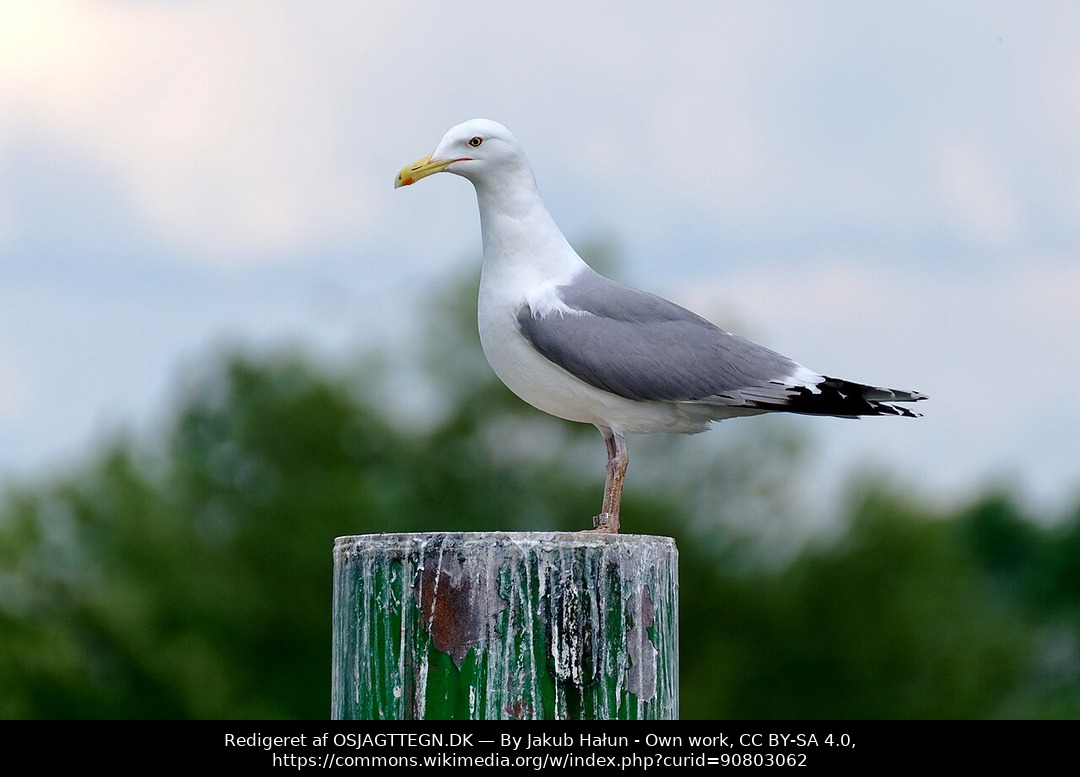
\includegraphics[width=\linewidth, height=7.2cm, keepaspectratio]{Billeder/Dyr/Fugle/Mågefugle/sølvmåge/soelvmaage-01.jpg}
  \end{columns}
\end{frame}
% ========== HÆTTEMÅGE (SOMMERDRAGT) ==========
\begin{frame}{%
  \begin{minipage}[c]{0.30\textwidth}
    Hættemåge\\[-0.1em]
    {\footnotesize (Sommerdragt)}
  \end{minipage}%
  \hfill
  \begin{minipage}[c]{0.45\textwidth}
    \footnotesize
    \textbf{Jagttid:} Ingen jagttid
  \end{minipage}%
  \hfill
  \begin{minipage}[c]{0.15\textwidth}
    \noindent\raggedleft
    
\includegraphics[width=0.5cm, height=0.5cm, keepaspectratio]{Billeder/Ikoner/star.png}
  \end{minipage}%
}
  \vspace{0.25em}
  \begin{columns}[T]
    \column{0.45\textwidth}
    \setlength{\parskip}{0.5em}
    \tiny
    \RaggedRight
    \textbf{\textit{Chroicocephalus ridibundus}} – lille, slank måge med hvidlig vingeforkant \par
    \textbf{Udseende:}\\
    \quad – Mørkebrun hætte som ikke går ned i nakken \\
    \quad – Rødt næb og røde ben \\
    \quad – Hvid krop med grå overside
    \column{0.52\textwidth}
    \centering
    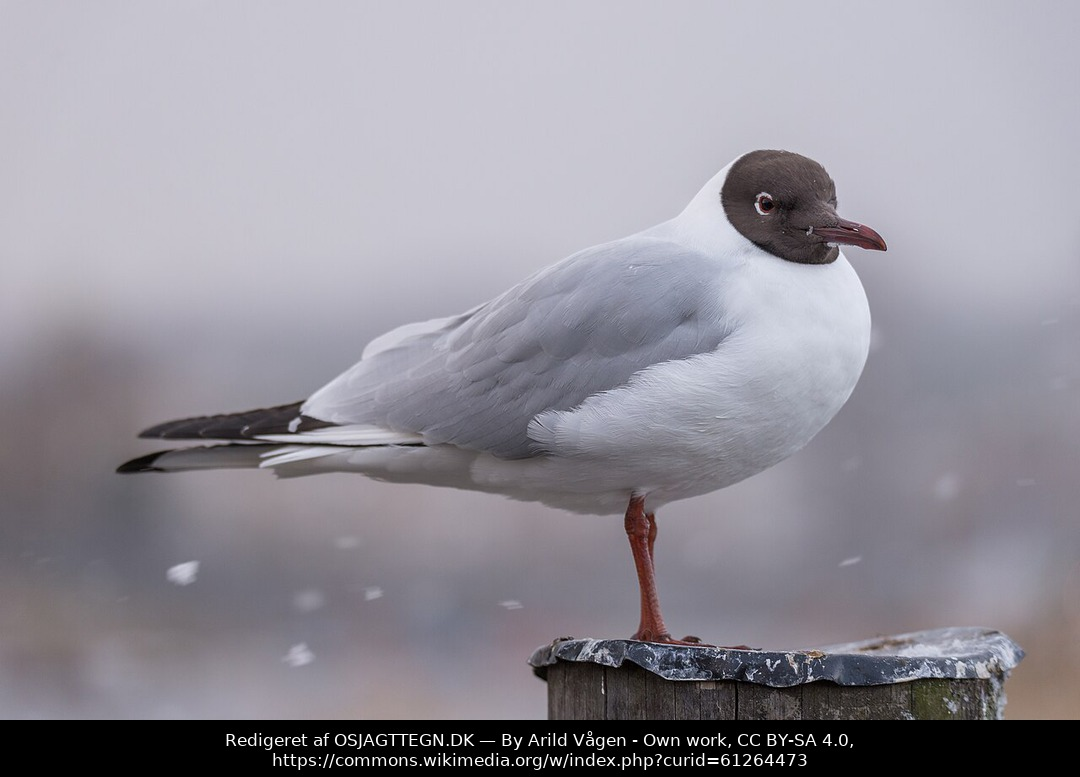
\includegraphics[width=\linewidth, height=7.2cm, keepaspectratio]{Billeder/Dyr/Fugle/Mågefugle/hættemåge/sommer.jpg}
  \end{columns}
\end{frame}

% ========== HÆTTEMÅGE (VINTERDRAGT) ==========
\begin{frame}{%
  \begin{minipage}[c]{0.30\textwidth}
    Hættemåge\\[-0.1em]
    {\footnotesize(Vinterdragt)}
  \end{minipage}%
  \hfill
  \begin{minipage}[c]{0.45\textwidth}
    \footnotesize
    \textbf{Jagttid:} Ingen jagttid
  \end{minipage}%
  \hfill
  \begin{minipage}[c]{0.15\textwidth}
    \noindent\raggedleft
    
\includegraphics[width=0.5cm, height=0.5cm, keepaspectratio]{Billeder/Ikoner/star.png}
  \end{minipage}%
}
  \vspace{0.25em}
  \begin{columns}[T]
    \column{0.45\textwidth}
    \setlength{\parskip}{0.5em}
    \tiny
    \RaggedRight
    \textbf{\textit{Chroicocephalus ridibundus}} – lille, slank måge med hvidlig vingeforkant \par
    \textbf{Udseende:}\\
    \quad – Ingen mørk hætte \\
    \quad – Mørkebrun plet bag øjet \\
    \quad – Hvidt hoved og hvid krop med grå overside
    \column{0.52\textwidth}
    \centering
    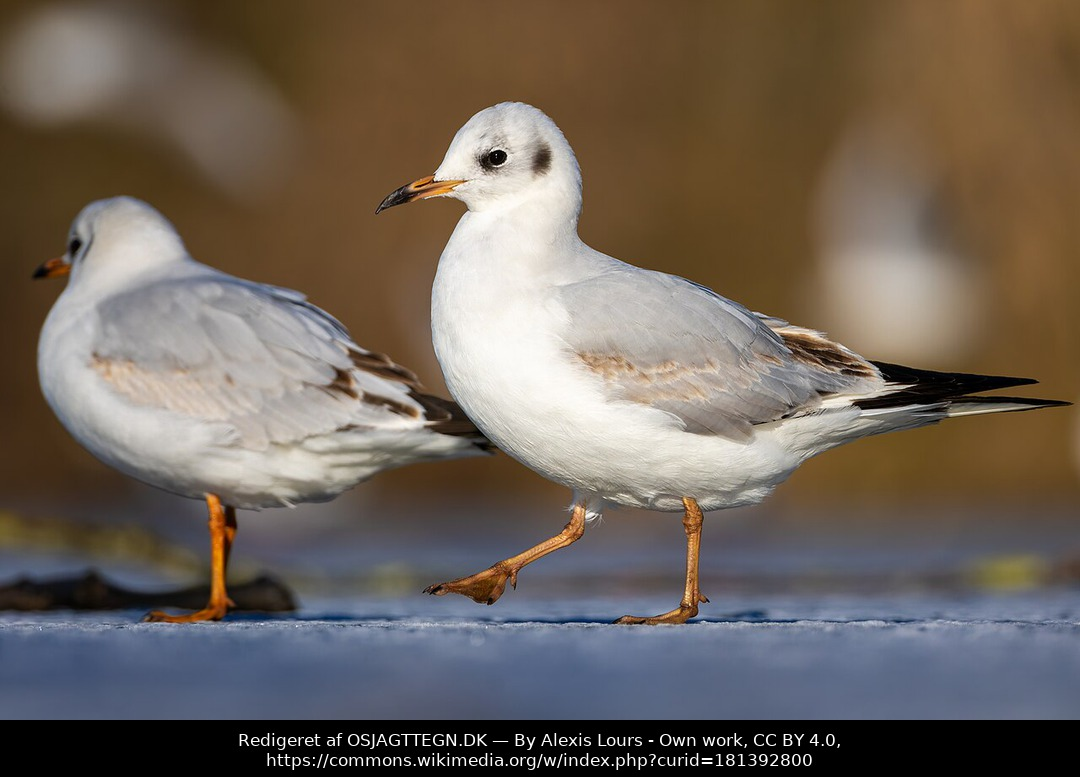
\includegraphics[width=\linewidth, height=7.2cm, keepaspectratio]{Billeder/Dyr/Fugle/Mågefugle/hættemåge/vinter.jpg}
  \end{columns}
\end{frame}
% ========== SILDEMÅGE ==========
\begin{frame}{%
  \begin{minipage}[c]{0.30\textwidth}
    Sildemåge
  \end{minipage}%
  \hfill
  \begin{minipage}[c]{0.45\textwidth}
    \footnotesize
    \textbf{Jagttid:} Ingen jagttid
  \end{minipage}%
  \hfill
  \begin{minipage}[c]{0.15\textwidth}
    \noindent\raggedleft
    
\includegraphics[width=0.5cm, height=0.5cm, keepaspectratio]{Billeder/Ikoner/star.png}
  \end{minipage}%
}
  \vspace{0.25em}
  \begin{columns}[T]
    \column{0.45\textwidth}
    \setlength{\parskip}{0.5em}
    \tiny
    \RaggedRight
    \textbf{\textit{Larus fuscus}} – mellemstor måge der ligner lille svartbag \par
    \textbf{Udseende:}\\
    \quad – Sort/mørk ryg og overvinger \\
    \quad – Hvide pletter på halefjerene \\
    \quad – Gule ben
    \column{0.52\textwidth}
    \centering
    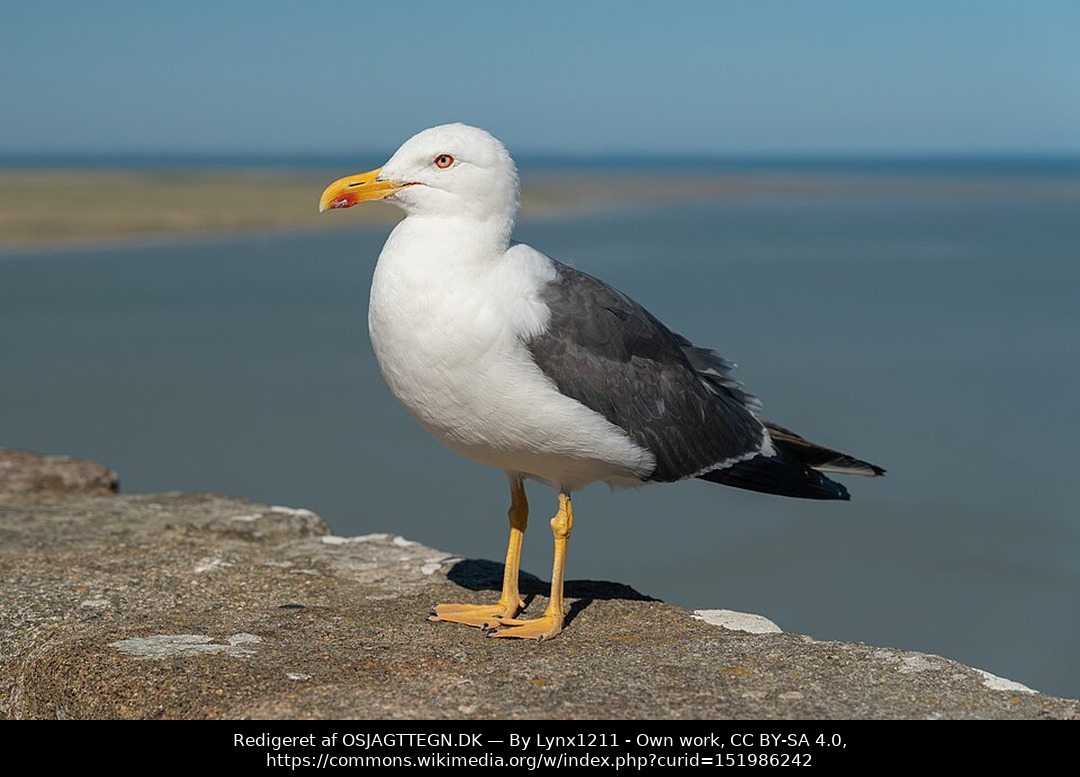
\includegraphics[width=\linewidth, height=7.2cm, keepaspectratio]{Billeder/Dyr/Fugle/Mågefugle/sildemåge/sildemaage-01.jpg}
  \end{columns}
\end{frame}
% ========== STORMMÅGE ==========
\begin{frame}{%
  \begin{minipage}[c]{0.30\textwidth}
    Stormmåge
  \end{minipage}%
  \hfill
  \begin{minipage}[c]{0.45\textwidth}
    \footnotesize
    \textbf{Jagttid:} Ingen jagttid
  \end{minipage}%
  \hfill
  \begin{minipage}[c]{0.15\textwidth}
    \noindent\raggedleft
    
\includegraphics[width=0.5cm, height=0.5cm, keepaspectratio]{Billeder/Ikoner/star.png}
  \end{minipage}%
}
  \vspace{0.25em}
  \begin{columns}[T]
    \column{0.45\textwidth}
    \setlength{\parskip}{0.5em}
    \tiny
    \RaggedRight
    \textbf{\textit{Larus canus}} – lille til mellemstor måge \par
    \textbf{Udseende:}\\
    \quad – Rundt hoved \\
    \quad – Mørkt øje (ser venlig ud) \\
    \quad – Slankt næb
    \column{0.52\textwidth}
    \centering
    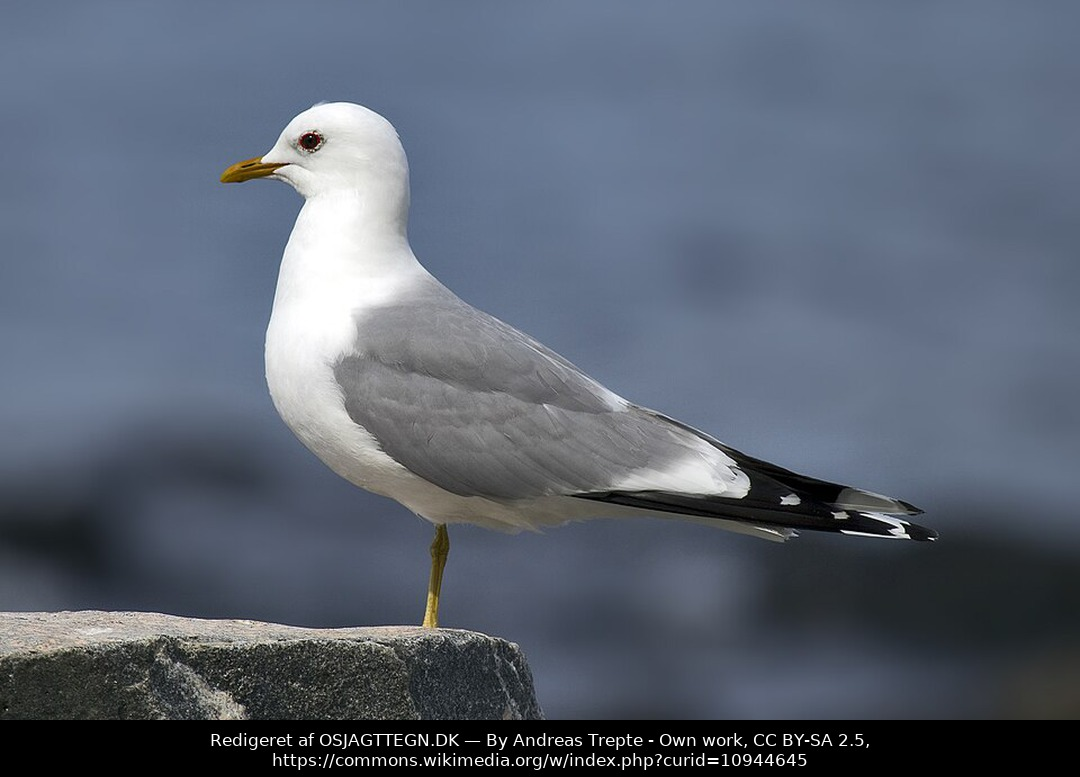
\includegraphics[width=\linewidth, height=7.2cm, keepaspectratio]{Billeder/Dyr/Fugle/Mågefugle/stormmåge/stormmaage-05.jpg}
  \end{columns}
\end{frame}
% ========== SVARTBAG ==========
\begin{frame}{%
  \begin{minipage}[c]{0.30\textwidth}
    Svartbag
  \end{minipage}%
  \hfill
  \begin{minipage}[c]{0.45\textwidth}
    \footnotesize
    \textbf{Jagttid:} Ingen jagttid
  \end{minipage}%
  \hfill
  \begin{minipage}[c]{0.15\textwidth}
    \noindent\raggedleft
    
\includegraphics[width=0.5cm, height=0.5cm, keepaspectratio]{Billeder/Ikoner/star.png}
  \end{minipage}%
}
  \vspace{0.25em}
  \begin{columns}[T]
    \column{0.45\textwidth}
    \setlength{\parskip}{0.5em}
    \tiny
    \RaggedRight
    \textbf{\textit{Larus marinus}} – meget stor og kraftig måge \par
    \textbf{Udseende:}\\
    \quad – Sort ryg og vingeoversider \\
    \quad – Hvide pletter på halen (blinklys) \\
    \quad – Lyserøde ben \\
    \quad – Kraftigt, ``fortrykket'' næb
    \column{0.52\textwidth}
    \centering
    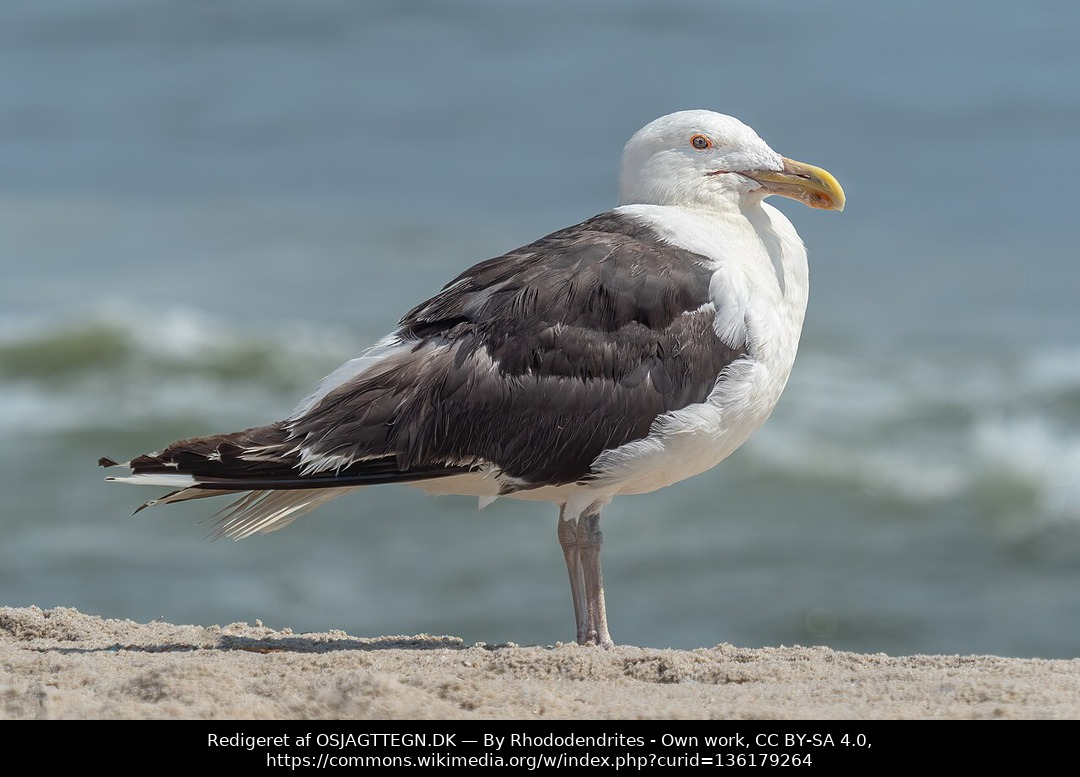
\includegraphics[width=\linewidth, height=7.2cm, keepaspectratio]{Billeder/Dyr/Fugle/Mågefugle/svartbag/svartbag-01.jpg}
  \end{columns}
\end{frame}
\begin{frame}
  \vspace{1.8em}
  \begin{center}
    \begin{minipage}{0.22\textwidth}
      \centering
      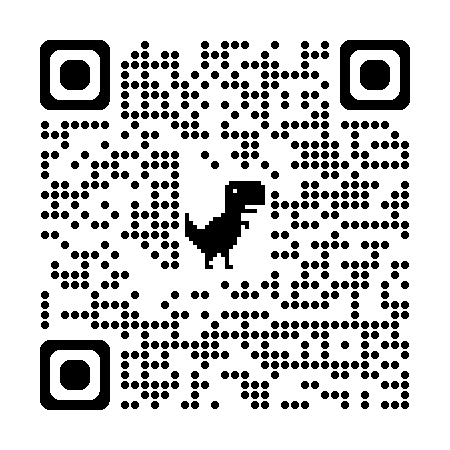
\includegraphics[width=\linewidth]{Billeder/Dyr/Fugle/Mågefugle/qr/maagefugle_qr.png}
    \end{minipage}%
    \hspace{0.8em}%
    \begin{minipage}{0.62\textwidth}
      \raggedright
      \Large
      \textbf{Træning i artsbestemmelse af mågefugle}\\[0.35em]
      {\large https://osjagttegn.dk/maagefugle}
    \end{minipage}
  \end{center}
\end{frame}

%\section{Vandhøns (vildtkending og biologi)}

% ========== TITEL: VANDHØNS ==========
\begin{frame}
  \vspace{1.5em}
  \begin{center}
    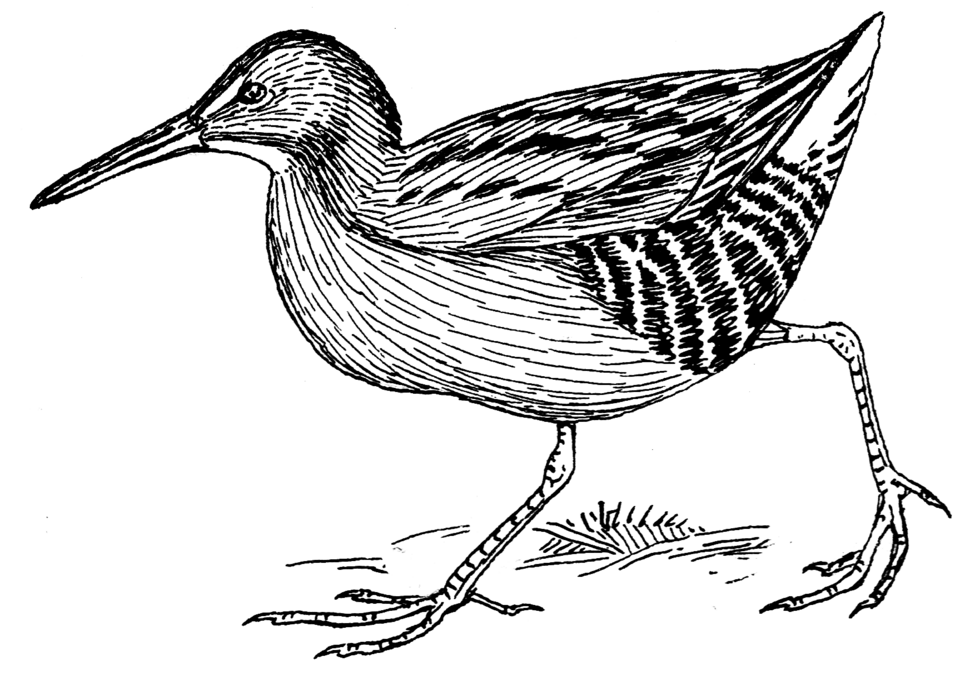
\includegraphics[width=12cm, height=4cm, keepaspectratio]{Billeder/Dyr/Fugle/Vandhøns/vandhøns.png}\\[1.2em]
    {\LARGE \textbf{Vandhøns}}\\[0.6em]
   
    Artsbestemmelse \& vildtbiologi\\[0.9em]
    {\tiny\color{gray}
    CC BY 4.0 – kan frit anvendes, også kommercielt. Rettighederne må ikke skærpes.\\[0.05em]
    Udviklet af Aleksander Sønder, OSJAGTTEGN.DK}
  \end{center}
\end{frame}

% ========== BLISHØNE ==========
\begin{frame}{%
  \begin{minipage}[c]{0.30\textwidth}
    Blishøne
  \end{minipage}%
  \hfill
  \begin{minipage}[c]{0.45\textwidth}
    \footnotesize
    \textbf{Jagttid:} 1.\ oktober -- 31.\ januar
  \end{minipage}%
  \hfill
  \begin{minipage}[c]{0.15\textwidth}
    \noindent\raggedleft
    
\includegraphics[width=0.5cm, height=0.5cm, keepaspectratio]{Billeder/Ikoner/star.png}%
    \hspace{0.2em}%
    
\includegraphics[width=0.5cm, height=0.5cm, keepaspectratio]{Billeder/Ikoner/star.png}
  \end{minipage}%
}
  \vspace{0.25em}
  \begin{columns}[T]
    \column{0.45\textwidth}
    \setlength{\parskip}{0.5em}
    \tiny
    \RaggedRight
    \textbf{\textit{Fulica atra}} – kraftig vandfugl med rund, skifersort krop og lange ben \par
    \textbf{Udseende:}\\
    \quad – Sort fjerdragt \\
    \quad – Hvid pandeblis \\
    \quad – Næb med rosa spids \par
    \textbf{Levesteder:} Søer og indre farvande. \par
    \textbf{Føde:} Vandplanter suppleret med muslinger, insekter og bløddyr. \par
    \textbf{Udbredelse:} Hele Danmark. \par
    \textbf{Træk/standfugl:} Begge
    \column{0.52\textwidth}
    \centering
    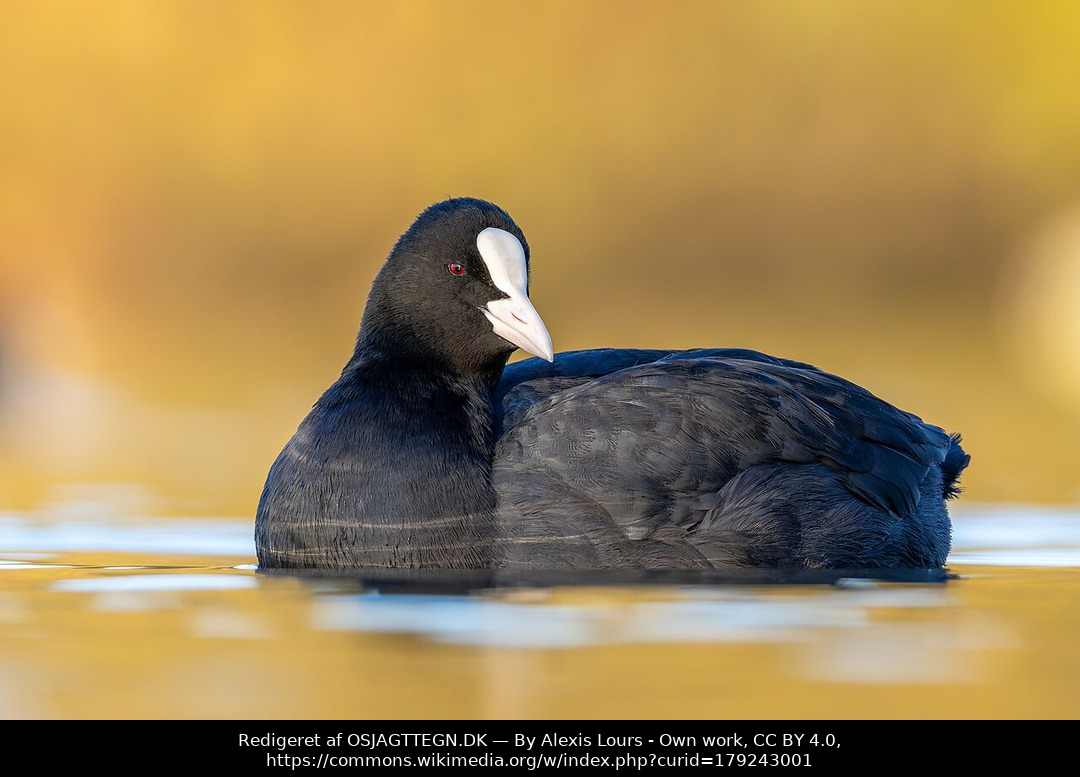
\includegraphics[width=\linewidth, height=7.2cm, keepaspectratio]{Billeder/Dyr/Fugle/Vandhøns/blishoene-01.jpg}
  \end{columns}
\end{frame}
% ========== GRØNBENET RØRHØNE ==========
\begin{frame}{%
  \begin{minipage}[c]{0.30\textwidth}
    Grønbenet rørhøne
  \end{minipage}%
  \hfill
  \begin{minipage}[c]{0.45\textwidth}
    \footnotesize
    \textbf{Jagttid:} Ingen jagttid
  \end{minipage}%
  \hfill
  \begin{minipage}[c]{0.15\textwidth}
    \noindent\raggedleft
    
\includegraphics[width=0.5cm, height=0.5cm, keepaspectratio]{Billeder/Ikoner/star.png}
  \end{minipage}%
}
  \vspace{0.25em}
  \begin{columns}[T]
    \column{0.45\textwidth}
    \setlength{\parskip}{0.5em}
    \tiny
    \RaggedRight
    \textbf{\textit{Gallinula chloropus}} – slankere end blishønen \par
    \textbf{Udseende:}\\
    \quad – Sort med hvid flankestribe \\
    \quad – Rødt næb med gul spids \\
    \quad – Rødt pandeskjold og grønlige ben
    \column{0.52\textwidth}
    \centering
    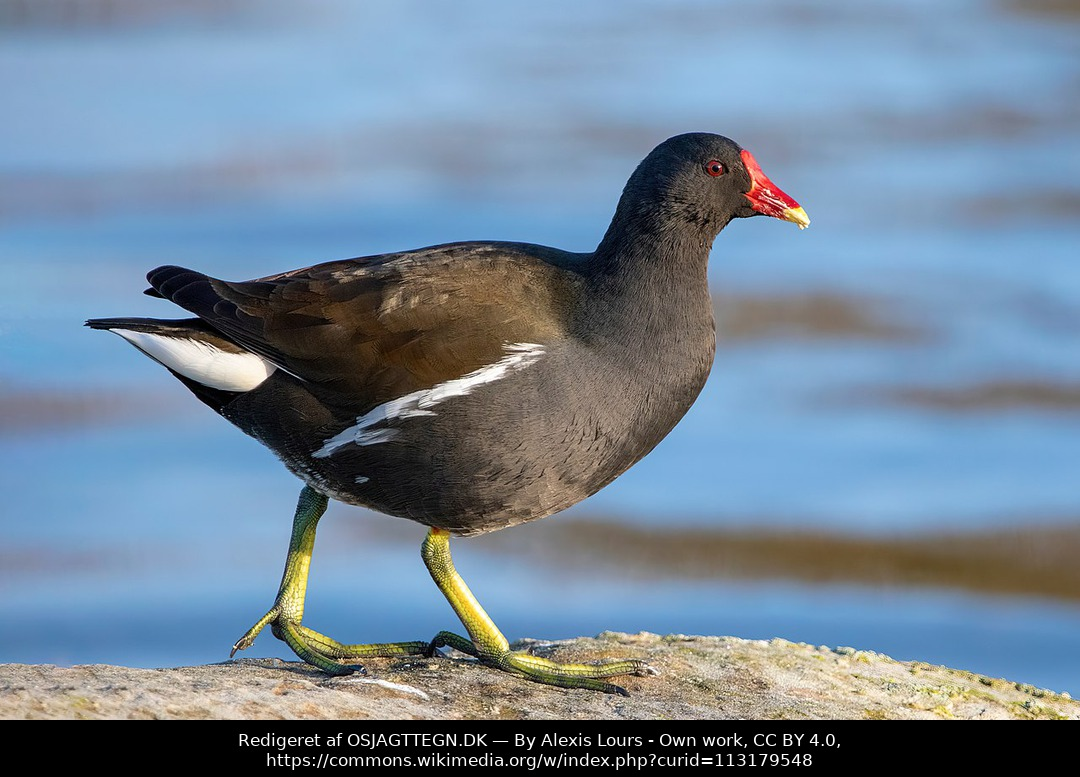
\includegraphics[width=\linewidth, height=7.2cm, keepaspectratio]{Billeder/Dyr/Fugle/Vandhøns/groenbenetroerhoene-02.jpg}
  \end{columns}
\end{frame}
\begin{frame}
  \vspace{1.8em}
  \begin{center}
    \begin{minipage}{0.22\textwidth}
      \centering
      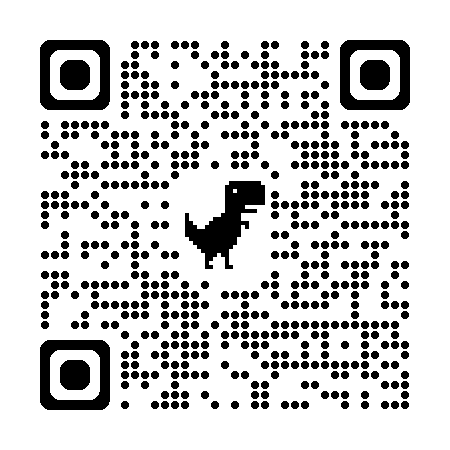
\includegraphics[width=\linewidth]{Billeder/Dyr/Fugle/Vandhøns/qr/vandhøns_qr.png}
    \end{minipage}%
    \hspace{0.8em}%
    \begin{minipage}{0.62\textwidth}
      \raggedright
      \Large
      \textbf{Træning i artsbestemmelse af vandhøns}\\[0.35em]
      {\large https://osjagttegn.dk/vandhoens}
    \end{minipage}
  \end{center}
\end{frame}

%% ========== TITEL: SPURVEFUGLE ==========
\begin{frame}
  \vspace{1.5em}
  \begin{center}
    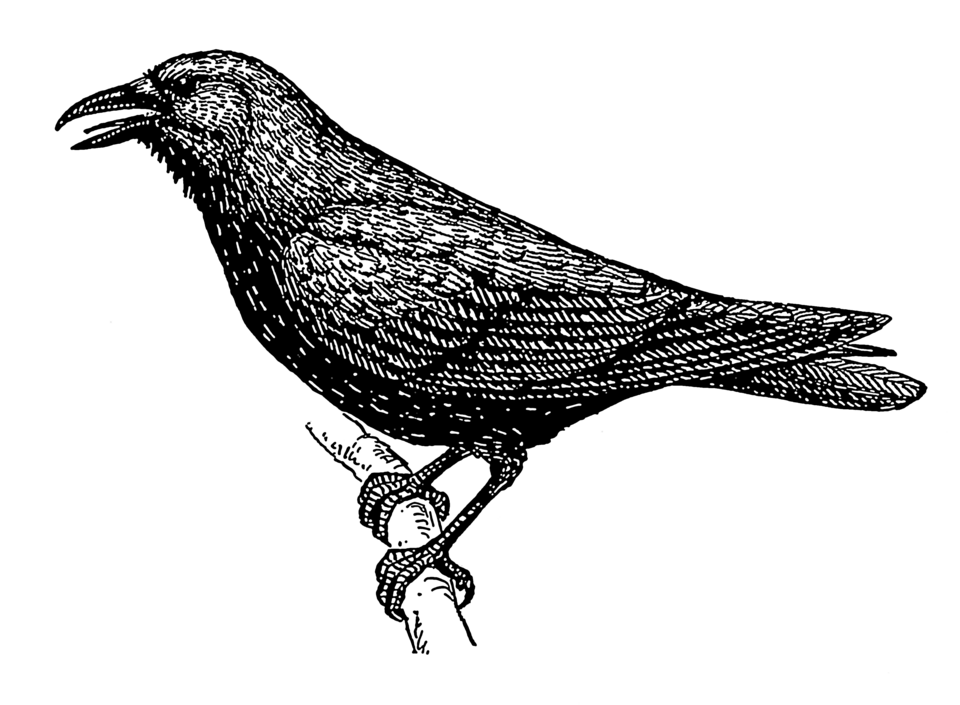
\includegraphics[width=12cm, height=4cm, keepaspectratio]{Billeder/Dyr/Fugle/Spurvefugle/spurvefugle.png}\\[1.2em]
    {\LARGE \textbf{Spurvefugle}}\\[0.6em]
    Artsbestemmelse \& vildtbiologi \\[0.9em]
    {\tiny\color{gray}
    CC BY 4.0 – kan frit anvendes, også kommercielt. Rettighederne må ikke skærpes.\\[0.05em]
    Udviklet af Aleksander Sønder, OSJAGTTEGN.DK}
  \end{center}
\end{frame}

\section{Spurvefugle/Kragefugle (vildtkending og biologi)}

% ========== SORTKRAGE ==========
\begin{frame}{%
  \begin{minipage}[c]{0.30\textwidth}
    Sortkrage (Krage)
  \end{minipage}%
  \hfill
  \begin{minipage}[c]{0.45\textwidth}
    \footnotesize
    \textbf{Jagttid:} 1.\ september -- 31.\ januar
  \end{minipage}%
  \hfill
  \begin{minipage}[c]{0.15\textwidth}
    \noindent\raggedleft
    
\includegraphics[width=0.5cm, height=0.5cm, keepaspectratio]{Billeder/Ikoner/star.png}%
    \hspace{0.2em}%
    
\includegraphics[width=0.5cm, height=0.5cm, keepaspectratio]{Billeder/Ikoner/star.png}%
    \hspace{0.2em}%
    
\includegraphics[width=0.5cm, height=0.5cm, keepaspectratio]{Billeder/Ikoner/star.png}
  \end{minipage}%
}
  \vspace{0.25em}
  \begin{columns}[T]
    \column{0.45\textwidth}
    \setlength{\parskip}{0.45em}
    \tiny
    \RaggedRight
    \textbf{\textit{Corvus corone}} – mellemstor kragefugl, nært beslægtet med gråkrage \par
    \textbf{Udseende:}\\
    \quad – Heltsort krop og hoved \\
    \quad – Sorte øjne \\
    \quad – Ligner ravn, men er mindre og har slankere næb \par
    \textbf{Levesteder:} Alle landskabstyper. \par
    \textbf{Føde:} Opportunist – spiser alt, inkl.\ yngel. \par
    \textbf{Udbredelse:} Især Vestjylland. Sjældnere i resten af landet. \par
    \textbf{Træk/standfugl:} Begge \par
    \textbf{Forplantning:}\\
    \quad – \textbf{Yngleforhold:} Yngler i høje træer. Parret forsvarer territoriet \\
    \quad – \textbf{Kønsmoden:} 2 år \\
    \quad – \textbf{Mono/polygam:} Monogam \\
    \quad – \textbf{Bestandsomsætning:} Langsom \\
    \quad – \textbf{Kuld:} 4--6 æg
    \column{0.52\textwidth}
    \centering
    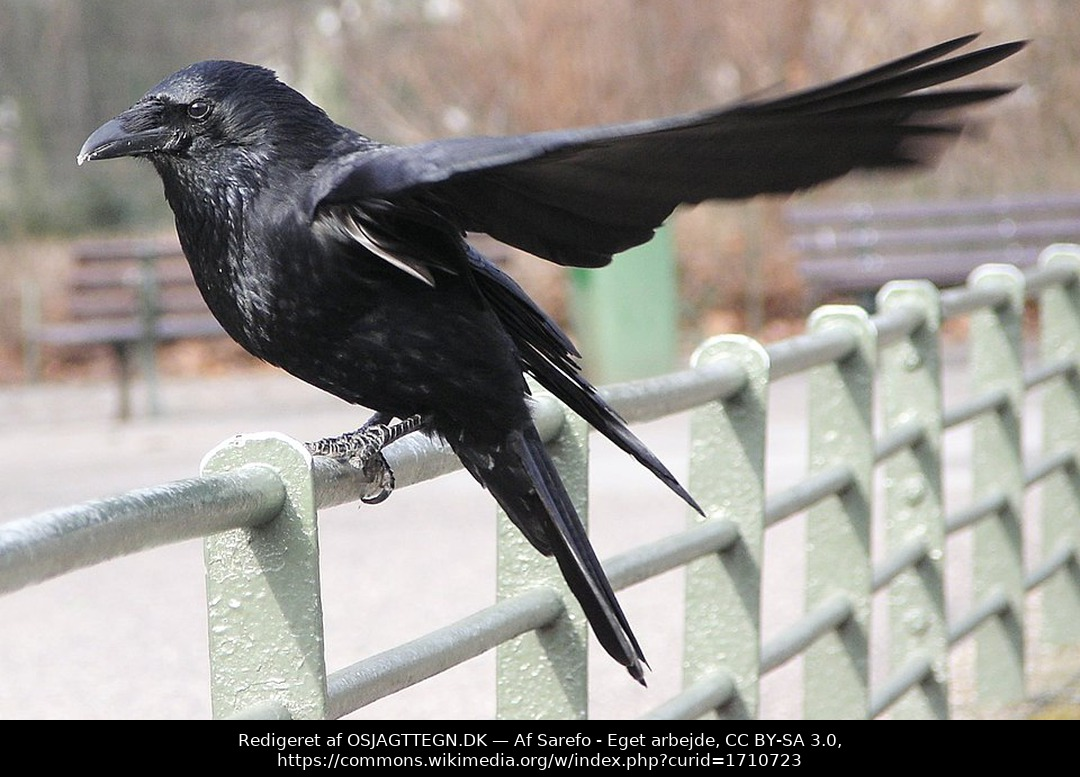
\includegraphics[width=\linewidth, height=7.2cm, keepaspectratio]{Billeder/Dyr/Fugle/Spurvefugle/sortkrage-01.jpg}
  \end{columns}
\end{frame}
% ========== GRÅKRAGE ==========
\begin{frame}{%
  \begin{minipage}[c]{0.30\textwidth}
    Gråkrage (Krage)
  \end{minipage}%
  \hfill
  \begin{minipage}[c]{0.45\textwidth}
    \footnotesize
    \textbf{Jagttid:} 1.\ september -- 31.\ januar
  \end{minipage}%
  \hfill
  \begin{minipage}[c]{0.15\textwidth}
    \noindent\raggedleft
    
\includegraphics[width=0.5cm, height=0.5cm, keepaspectratio]{Billeder/Ikoner/star.png}%
    \hspace{0.2em}%
    
\includegraphics[width=0.5cm, height=0.5cm, keepaspectratio]{Billeder/Ikoner/star.png}%
    \hspace{0.2em}%
    
\includegraphics[width=0.5cm, height=0.5cm, keepaspectratio]{Billeder/Ikoner/star.png}
  \end{minipage}%
}
  \vspace{0.25em}
  \begin{columns}[T]
    \column{0.45\textwidth}
    \setlength{\parskip}{0.45em}
    \tiny
    \RaggedRight
    \textbf{\textit{Corvus cornix}} – mellemstor kragefugl, den almindeligste krage i Danmark \par
    \textbf{Udseende:}\\
    \quad – Grå krop \\
    \quad – Sort hoved, bryst og vinger \\
    \quad – Sorte øjne \par
    \textbf{Levesteder:} Alle landskabstyper. \par
    \textbf{Føde:} Opportunist – spiser alt, inkl.\ yngel. \par
    \textbf{Udbredelse:} Hele Danmark. \par
    \textbf{Træk/standfugl:} Begge \par
    \textbf{Forplantning:}\\
    \quad – \textbf{Yngleforhold:} Yngler i høje træer. Parret forsvarer territoriet \\
    \quad – \textbf{Kønsmoden:} 2 år \\
    \quad – \textbf{Mono/polygam:} Monogam \\
    \quad – \textbf{Bestandsomsætning:} Langsom \\
    \quad – \textbf{Kuld:} 4--6 æg
    \column{0.52\textwidth}
    \centering
    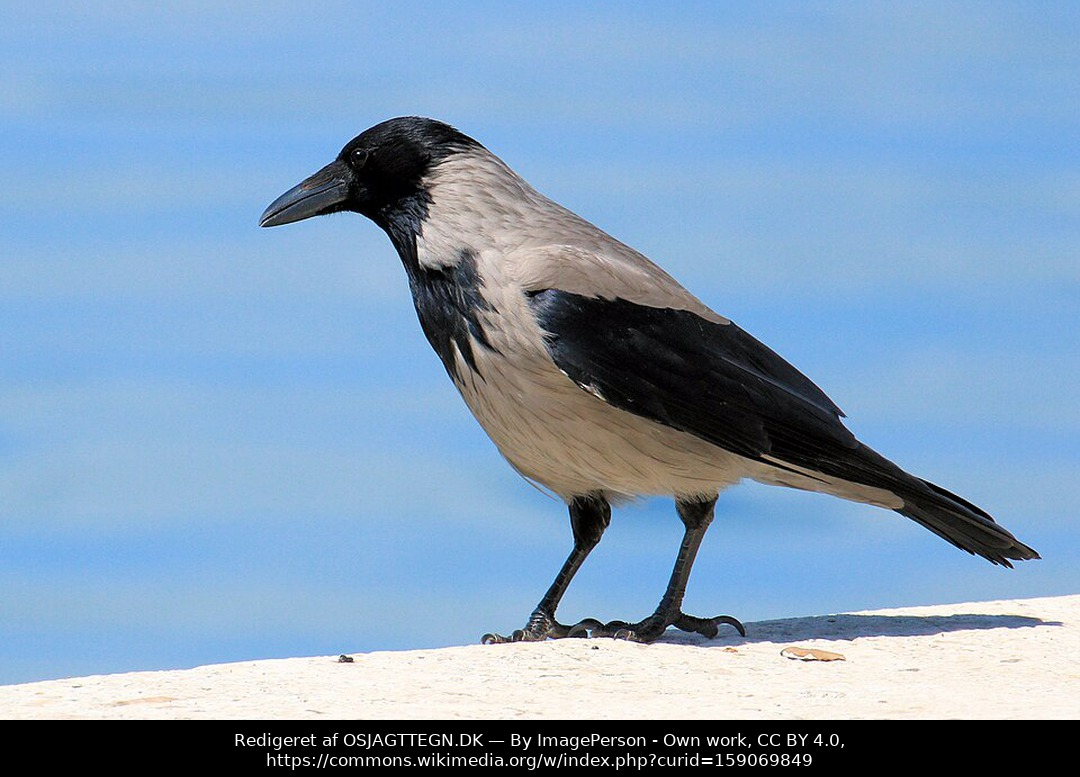
\includegraphics[width=\linewidth, height=7.2cm, keepaspectratio]{Billeder/Dyr/Fugle/Spurvefugle/graakrage-02.jpg}
  \end{columns}
\end{frame}

% ========== RAVN ==========
\begin{frame}{%
  \begin{minipage}[c]{0.30\textwidth}
    Ravn
  \end{minipage}%
  \hfill
  \begin{minipage}[c]{0.45\textwidth}
    \footnotesize
    \textbf{Jagttid:} Ingen jagttid
  \end{minipage}%
  \hfill
  \begin{minipage}[c]{0.15\textwidth}
    \noindent\raggedleft
    
\includegraphics[width=0.5cm, height=0.5cm, keepaspectratio]{Billeder/Ikoner/star.png}
  \end{minipage}%
}
  \vspace{0.25em}
  \begin{columns}[T]
    \column{0.45\textwidth}
    \setlength{\parskip}{0.5em}
    \tiny
    \RaggedRight
    \textbf{\textit{Corvus corax}} – stor, sort kragefugl med kraftigt næb \par
    \textbf{Udseende:}\\
    \quad – Heltsort fjerdragt \\
    \quad – Små fjer går ud på næbbet \\
    \quad – Kraftigere bygget end de øvrige kragefugle
    \column{0.52\textwidth}
    \centering
    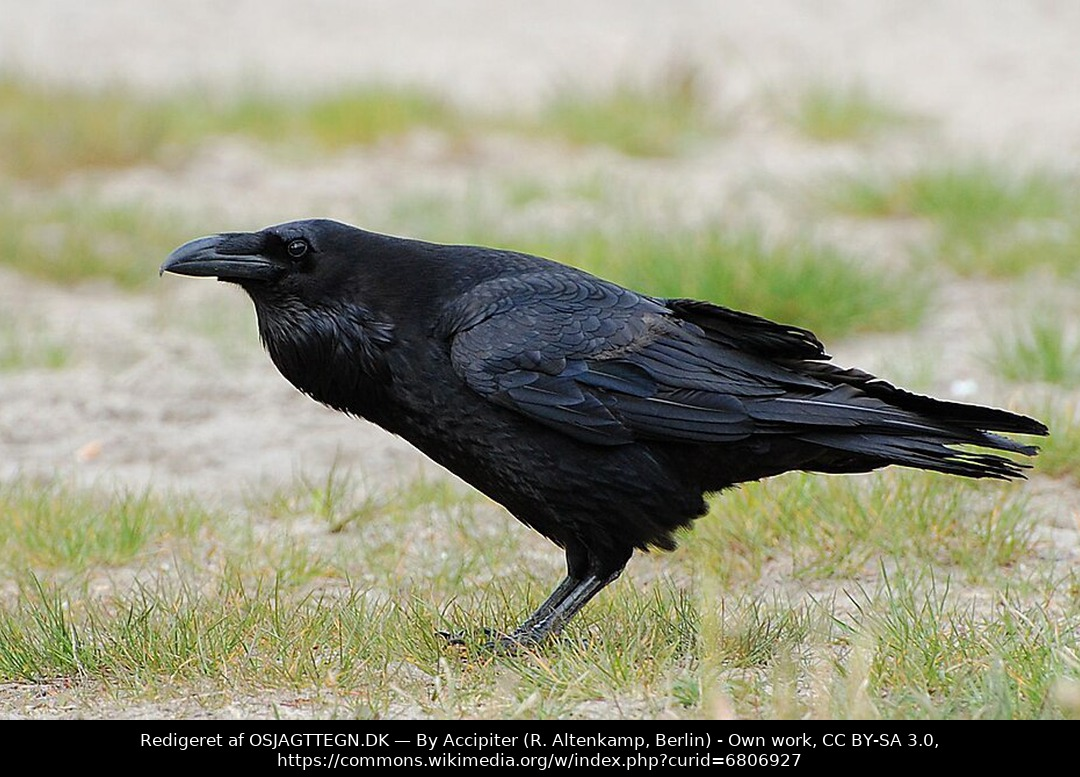
\includegraphics[width=\linewidth, height=7.2cm, keepaspectratio]{Billeder/Dyr/Fugle/Spurvefugle/ravn-01.jpg}
  \end{columns}
\end{frame}
% ========== RÅGE ==========
\begin{frame}{%
  \begin{minipage}[c]{0.30\textwidth}
    Råge
  \end{minipage}%
  \hfill
  \begin{minipage}[c]{0.45\textwidth}
    \footnotesize
    \textbf{Jagttid:} Ingen jagttid
  \end{minipage}%
  \hfill
  \begin{minipage}[c]{0.15\textwidth}
    \noindent\raggedleft
    
\includegraphics[width=0.5cm, height=0.5cm, keepaspectratio]{Billeder/Ikoner/star.png}%
    \hspace{0.2em}%
    
\includegraphics[width=0.5cm, height=0.5cm, keepaspectratio]{Billeder/Ikoner/star.png}
  \end{minipage}%
}
  \vspace{0.25em}
  \begin{columns}[T]
    \column{0.45\textwidth}
    \setlength{\parskip}{0.5em}
    \tiny
    \RaggedRight
    \textbf{\textit{Corvus frugilegus}} – kolonirugende kragefugl med fjerløs næbrod \par
    \textbf{Udseende:}\\
    \quad – Sort med metallisk skær \\
    \quad – Bart, gult eller gråligt parti ved næbbets rod \par
    \textbf{Levesteder:} Alle landskabstyper, men hyppigere ved byer. \par
    \textbf{Føde:} Plantemateriale suppleret med insekter og lignende. \par
    \textbf{Udbredelse:} Hele Danmark. \par
    \textbf{Træk/standfugl:} Standfugl
    \column{0.52\textwidth}
    \centering
    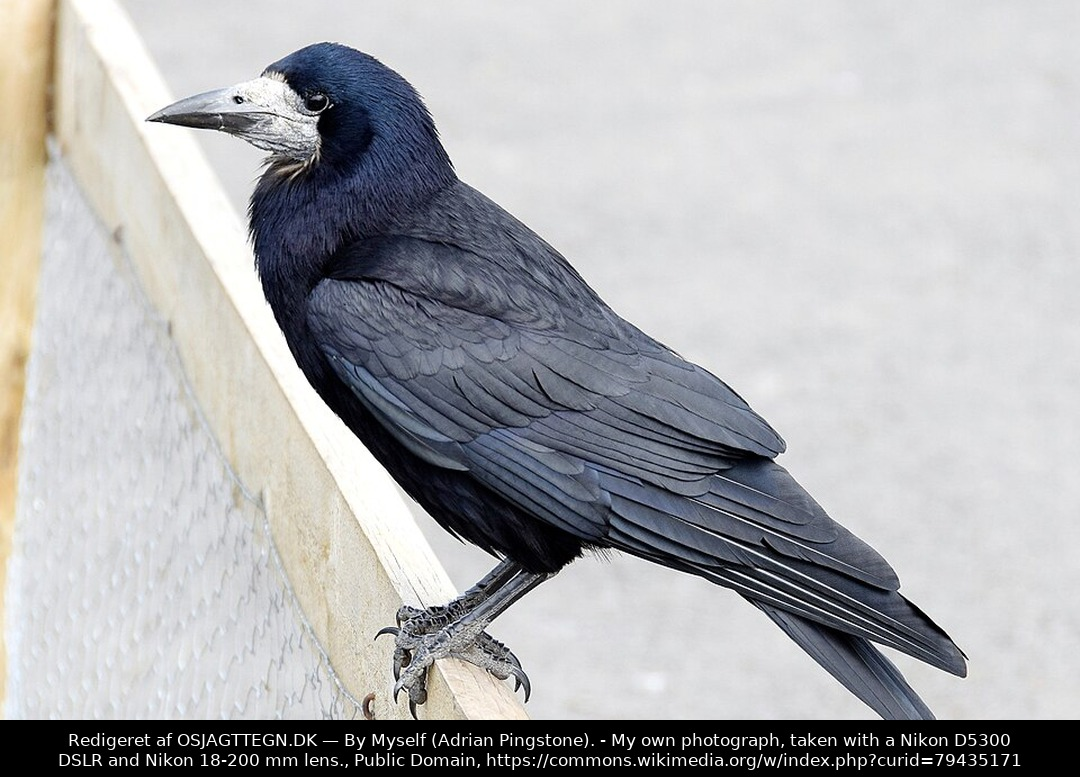
\includegraphics[width=\linewidth, height=7.2cm, keepaspectratio]{Billeder/Dyr/Fugle/Spurvefugle/raage-01.jpg}
  \end{columns}
\end{frame}
% ========== ALLIKE ==========
\begin{frame}{%
  \begin{minipage}[c]{0.30\textwidth}
    Allike
  \end{minipage}%
  \hfill
  \begin{minipage}[c]{0.45\textwidth}
    \footnotesize
    \textbf{Jagttid:} Ingen jagttid
  \end{minipage}%
  \hfill
  \begin{minipage}[c]{0.15\textwidth}
    \noindent\raggedleft
    
\includegraphics[width=0.5cm, height=0.5cm, keepaspectratio]{Billeder/Ikoner/star.png}
  \end{minipage}%
}
  \vspace{0.25em}
  \begin{columns}[T]
    \column{0.45\textwidth}
    \setlength{\parskip}{0.5em}
    \tiny
    \RaggedRight
    \textbf{\textit{Coloeus monedula}} – mindste kragefugl i Danmark med hvidgule øjne \par
    \textbf{Udseende:}\\
    \quad – Mindre end de andre kragefugle \\
    \quad – Grå nakke og hals \\
    \quad – Kendes især på det hvidgule øje
    \column{0.52\textwidth}
    \centering
    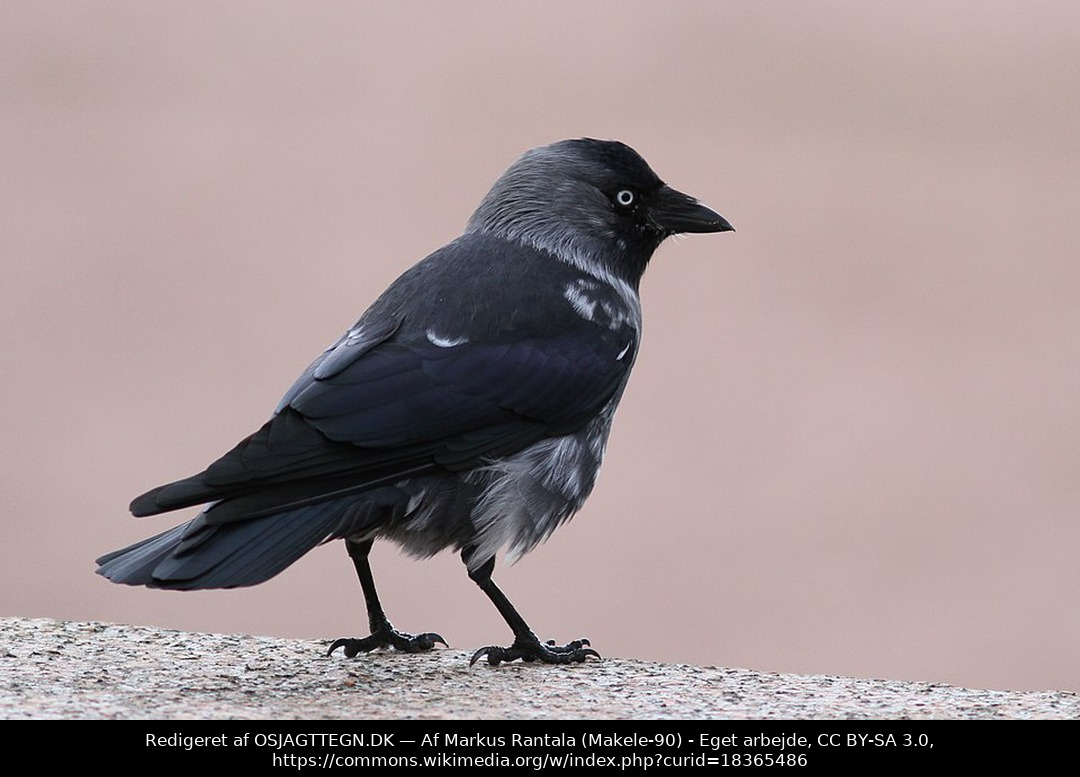
\includegraphics[width=\linewidth, height=7.2cm, keepaspectratio]{Billeder/Dyr/Fugle/Spurvefugle/allike-01.jpg}
  \end{columns}
\end{frame}
% ========== HUSSKADE ==========
\begin{frame}{%
  \begin{minipage}[c]{0.30\textwidth}
    Husskade
  \end{minipage}%
  \hfill
  \begin{minipage}[c]{0.45\textwidth}
    \footnotesize
    \textbf{Jagttid:} 1.\ september -- 31.\ januar
  \end{minipage}%
  \hfill
  \begin{minipage}[c]{0.15\textwidth}
    \noindent\raggedleft
    
\includegraphics[width=0.5cm, height=0.5cm, keepaspectratio]{Billeder/Ikoner/star.png}%
    \hspace{0.2em}%
    
\includegraphics[width=0.5cm, height=0.5cm, keepaspectratio]{Billeder/Ikoner/star.png}
  \end{minipage}%
}
  \vspace{0.25em}
  \begin{columns}[T]
    \column{0.45\textwidth}
    \setlength{\parskip}{0.5em}
    \tiny
    \RaggedRight
    \textbf{\textit{Pica pica}} – kendes på den lange hale og den sort-hvide fjerdragt \par
    \textbf{Udseende:}\\
    \quad – Sort og hvid med blågrønne metalskær \\
    \quad – Hoved og ryg sorte \\
    \quad – Bug og dele af vingerne hvide \par
    \textbf{Levesteder:} Alle landskabstyper, oftest i bynære zoner. \par
    \textbf{Føde:} Altædende. \par
    \textbf{Udbredelse:} Hele Danmark. \par
    \textbf{Træk/standfugl:} Standfugl
    \column{0.52\textwidth}
    \centering
    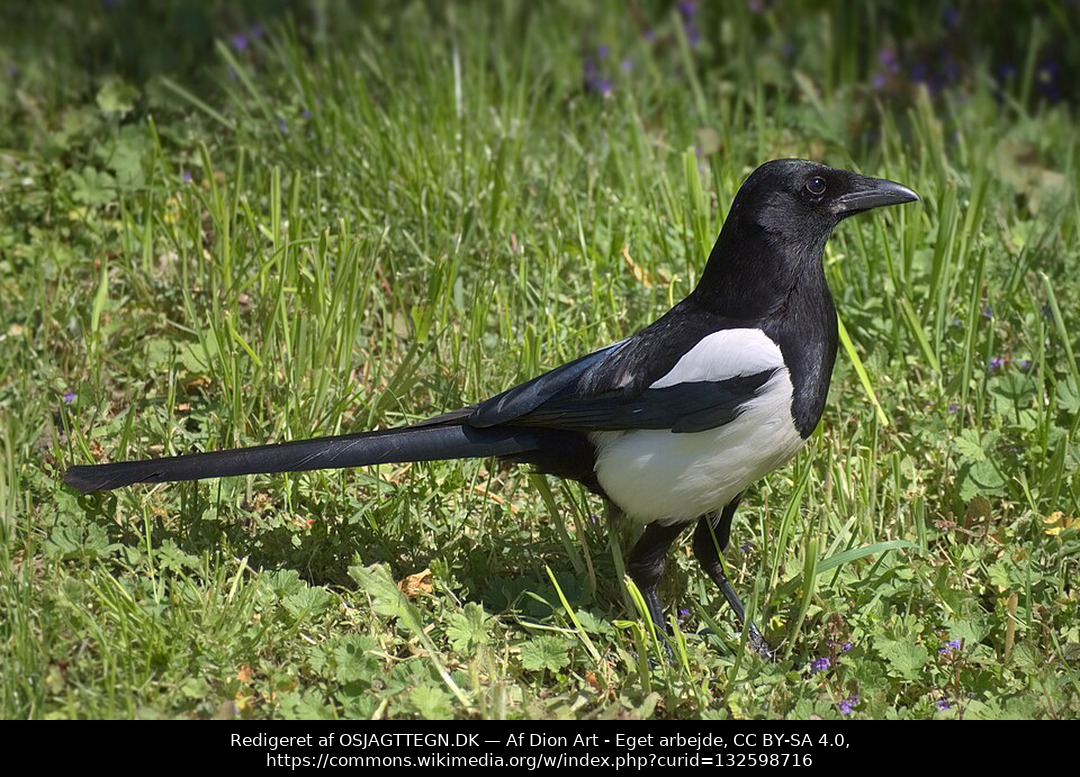
\includegraphics[width=\linewidth, height=7.2cm, keepaspectratio]{Billeder/Dyr/Fugle/Spurvefugle/husskade-01.jpg}
  \end{columns}
\end{frame}
% ========== SKOVSKADE ==========
\begin{frame}{%
  \begin{minipage}[c]{0.30\textwidth}
    Skovskade
  \end{minipage}%
  \hfill
  \begin{minipage}[c]{0.45\textwidth}
    \footnotesize
    \textbf{Jagttid:} Ingen jagttid
  \end{minipage}%
  \hfill
  \begin{minipage}[c]{0.15\textwidth}
    \noindent\raggedleft
    
\includegraphics[width=0.5cm, height=0.5cm, keepaspectratio]{Billeder/Ikoner/star.png}
  \end{minipage}%
}
  \vspace{0.25em}
  \begin{columns}[T]
    \column{0.45\textwidth}
    \setlength{\parskip}{0.5em}
    \tiny
    \RaggedRight
    \textbf{\textit{Garrulus glandarius}} – kendes på den rødbrune fjerdragt og det lyseblå felt på vingen \par
    \textbf{Udseende:}\\
    \quad – Rødbrun med hvid strube \\
    \quad – Sort hale \\
    \quad – Lyseblåt felt med sorte striber på vingen
    \column{0.52\textwidth}
    \centering
    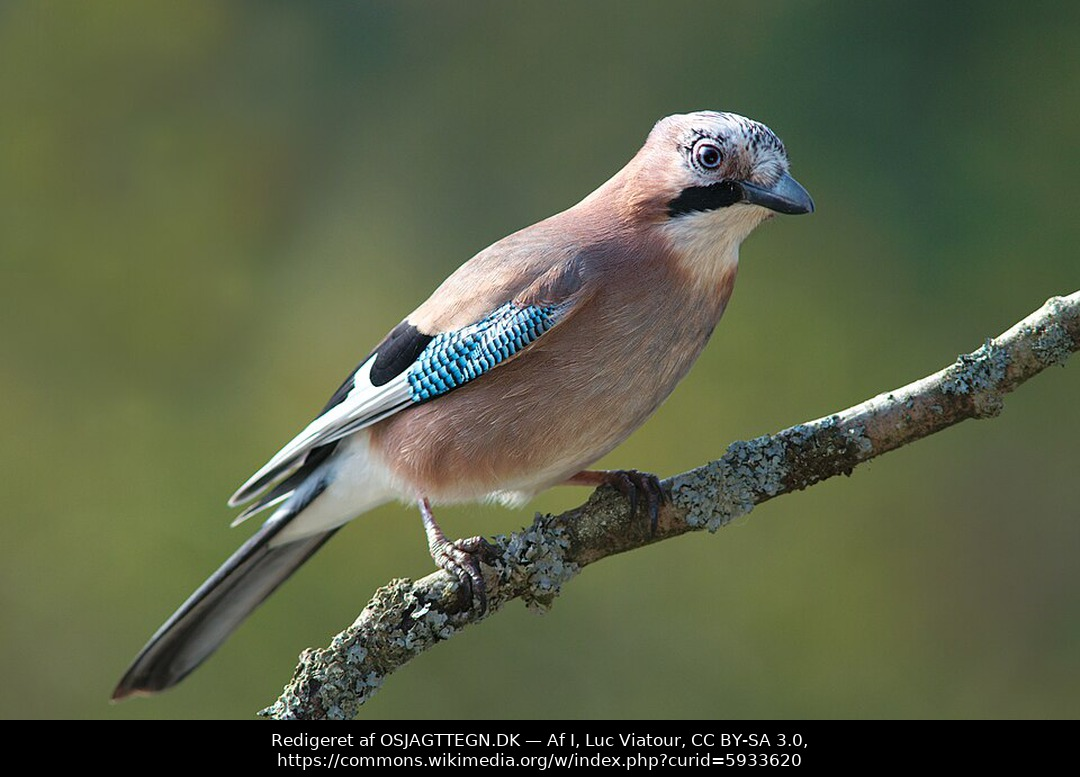
\includegraphics[width=\linewidth, height=7.2cm, keepaspectratio]{Billeder/Dyr/Fugle/Spurvefugle/skovskade-01.jpg}
  \end{columns}
\end{frame}

\begin{frame}
  \vspace{1.8em}
  \begin{center}
    \begin{minipage}{0.22\textwidth}
      \centering
      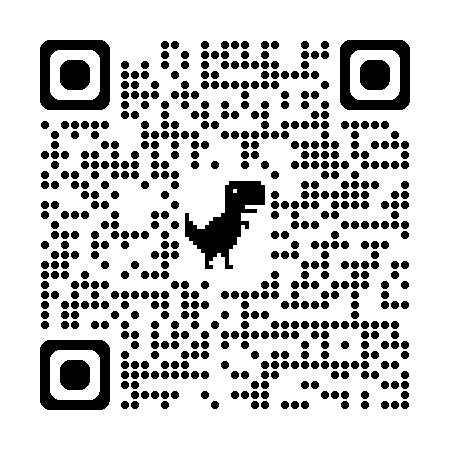
\includegraphics[width=\linewidth]{Billeder/Dyr/Fugle/Spurvefugle/qr/spurvefugle_qr.png}
    \end{minipage}%
    \hspace{0.8em}%
    \begin{minipage}{0.62\textwidth}
      \raggedright
      \Large
      \textbf{Træning i artsbestemmelse af spurvefugle}\\[0.35em]
      {\large https://osjagttegn.dk/spurvefugle}
    \end{minipage}
  \end{center}
\end{frame}

%% ========== TITEL: DUER ==========
\begin{frame}
  \vspace{1.5em}
  \begin{center}
    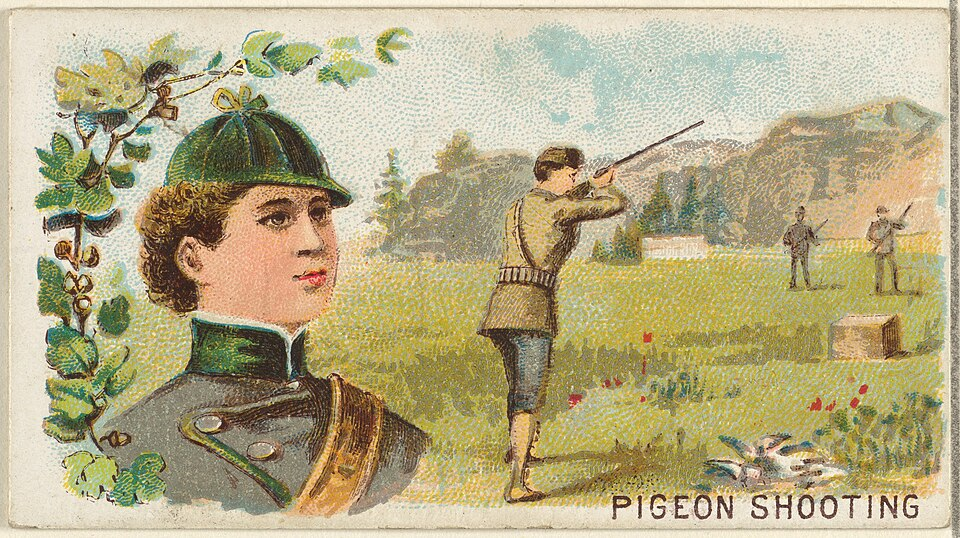
\includegraphics[width=12cm, height=4cm, keepaspectratio]{Billeder/Dyr/Fugle/Duer/duer.jpg}\\[1.2em]
    {\LARGE \textbf{Duer}}\\[0.6em]
    Artsbestemmelse \& vildtbiologi \\[0.9em]
    {\tiny\color{gray}
    CC BY 4.0 – kan frit anvendes, også kommercielt. Rettighederne må ikke skærpes.\\[0.05em]
    Udviklet af Aleksander Sønder, OSJAGTTEGN.DK}
  \end{center}
\end{frame}

\section{Duer (vildtkending og biologi)}

% ========== RINGDUE ==========
\begin{frame}{%
  \begin{minipage}[c]{0.30\textwidth}
    Ringdue
  \end{minipage}%
  \hfill
  \begin{minipage}[c]{0.45\textwidth}
    \footnotesize
    \textbf{Jagttid:} 11.\ november -- 31.\ januar
  \end{minipage}%
  \hfill
  \begin{minipage}[c]{0.15\textwidth}
    \noindent\raggedleft
    
\includegraphics[width=0.5cm, height=0.5cm, keepaspectratio]{Billeder/Ikoner/star.png}%
    \hspace{0.2em}%
    
\includegraphics[width=0.5cm, height=0.5cm, keepaspectratio]{Billeder/Ikoner/star.png}%
    \hspace{0.2em}%
    
\includegraphics[width=0.5cm, height=0.5cm, keepaspectratio]{Billeder/Ikoner/star.png}
  \end{minipage}%
}
  \vspace{0.25em}
  \begin{columns}[T]
    \column{0.45\textwidth}
    \setlength{\parskip}{0.45em}
    \tiny
    \RaggedRight
    \textbf{\textit{Columba palumbus}} – mest almindelige due i Danmark, også kaldet skovdue \par
    \textbf{Udseende:}\\
    \quad – Gråblå fjerdragt \\
    \quad – Hvid halsplet \\
    \quad – Gult næb \par
    \textbf{Levesteder:} Alle landskabstyper, hyppigst nær byer. \par
    \textbf{Føde:} Plantefrø og landbrugsafgrøder. \par
    \textbf{Udbredelse:} Hele Danmark. \par
    \textbf{Træk/standfugl:} Begge \par
    \textbf{Forplantning:}\\
    \quad – \textbf{Yngleforhold:} Bygger enkel rede af kviste \\
    \quad – \textbf{Kønsmoden:} 1 år \\
    \quad – \textbf{Mono/polygam:} Monogam \\
    \quad – \textbf{Bestandsomsætning:} Hurtig \\
    \quad – \textbf{Kuld:} 2 æg, 2--4 gange om året
    \column{0.52\textwidth}
    \centering
    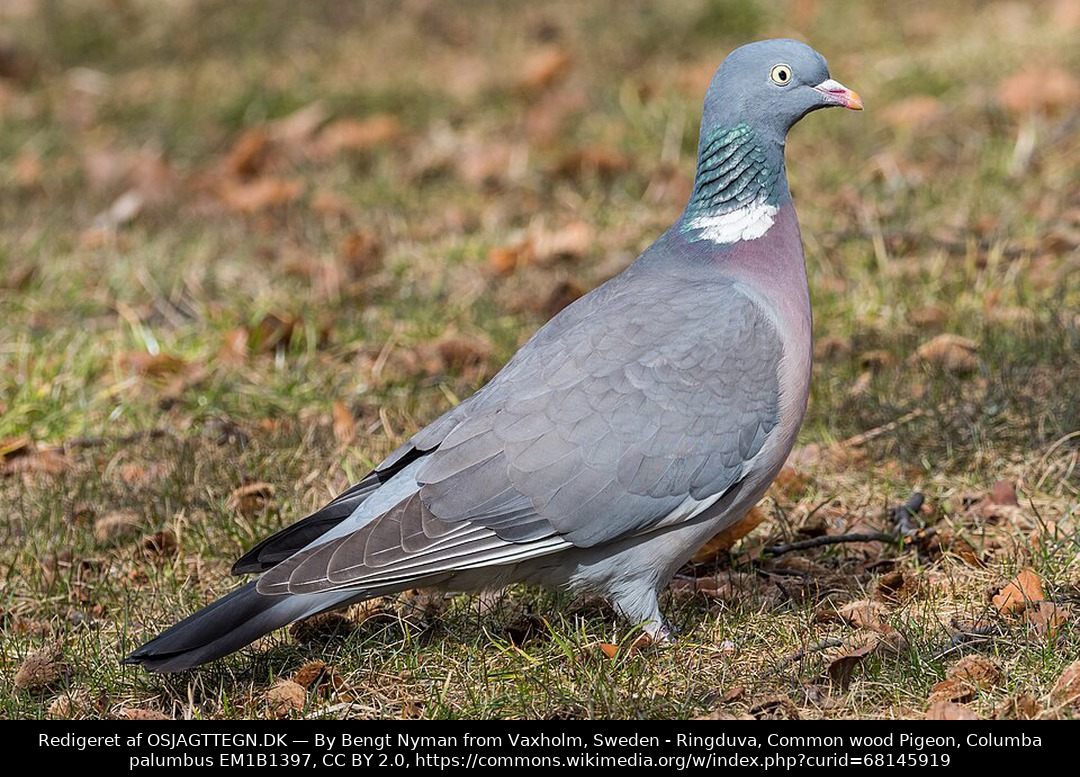
\includegraphics[width=\linewidth, height=7.2cm, keepaspectratio]{Billeder/Dyr/Fugle/Duer/ringdue-01.jpg}
  \end{columns}
\end{frame}
% ========== TYRKERDUE ==========
\begin{frame}{%
  \begin{minipage}[c]{0.30\textwidth}
    Tyrkerdue
  \end{minipage}%
  \hfill
  \begin{minipage}[c]{0.45\textwidth}
    \footnotesize
    \textbf{Jagttid:} Ingen jagttid
  \end{minipage}%
  \hfill
  \begin{minipage}[c]{0.15\textwidth}
    \noindent\raggedleft
    
\includegraphics[width=0.5cm, height=0.5cm, keepaspectratio]{Billeder/Ikoner/star.png}
  \end{minipage}%
}
  \vspace{0.25em}
  \begin{columns}[T]
    \column{0.45\textwidth}
    \setlength{\parskip}{0.5em}
    \tiny
    \RaggedRight
    \textbf{\textit{Streptopelia decaocto}} – lille, slank due \par
    \textbf{Udseende:}\\
    \quad – Lyst beigegrå eller sandfarvet \\
    \quad – Lang hale og forholdsvis smalle vinger med afrundede, mørke vingespidser \\
    \quad – Tydeligt sort, halvcirkelformet nakkebånd
    \column{0.52\textwidth}
    \centering
    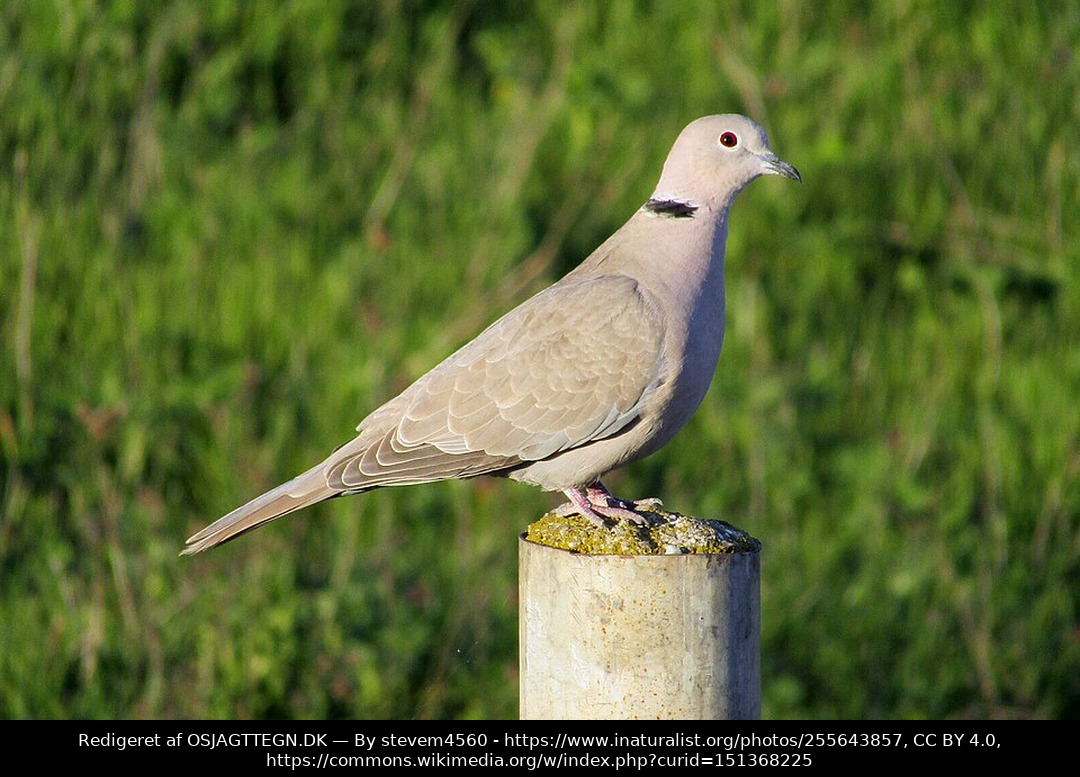
\includegraphics[width=\linewidth, height=7.2cm, keepaspectratio]{Billeder/Dyr/Fugle/Duer/tyrkerdue-01.jpg}
  \end{columns}
\end{frame}
% ========== HULDUE ==========
\begin{frame}{%
  \begin{minipage}[c]{0.30\textwidth}
    Huldue
  \end{minipage}%
  \hfill
  \begin{minipage}[c]{0.45\textwidth}
    \footnotesize
    \textbf{Jagttid:} Ingen jagttid
  \end{minipage}%
  \hfill
  \begin{minipage}[c]{0.15\textwidth}
    \noindent\raggedleft
    
\includegraphics[width=0.5cm, height=0.5cm, keepaspectratio]{Billeder/Ikoner/star.png}
  \end{minipage}%
}
  \vspace{0.25em}
  \begin{columns}[T]
    \column{0.45\textwidth}
    \setlength{\parskip}{0.5em}
    \tiny
    \RaggedRight
    \textbf{\textit{Columba oenas}} – fåtallig dansk ynglefugl, men temmelig almindelig som trækgæst. Den er fredet. \par
    \textbf{Udseende:}\\
    \quad – Rimelig ensfarvet, blålig fjerdragt \\
    \quad – Grønlig plet på halsen \\
    \quad – To sorte striber på hver vinge
    \column{0.52\textwidth}
    \centering
    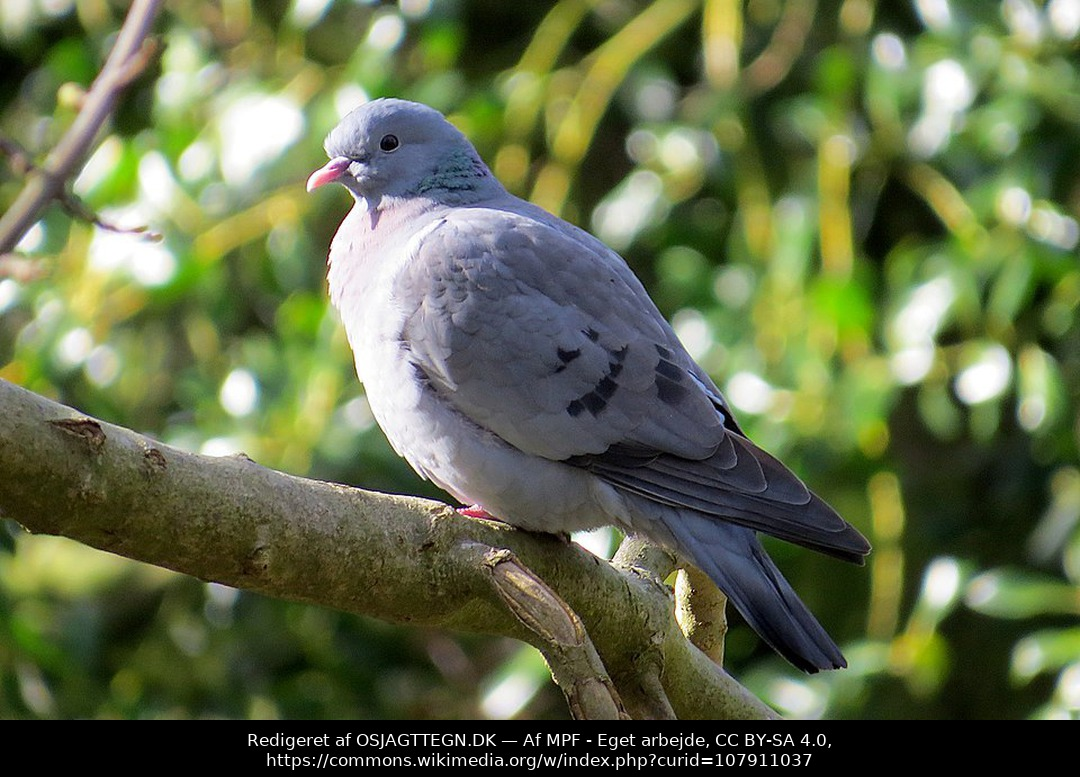
\includegraphics[width=\linewidth, height=7.2cm, keepaspectratio]{Billeder/Dyr/Fugle/Duer/huldue-01.jpg}
  \end{columns}
\end{frame}

\begin{frame}
  \vspace{1.8em}
  \begin{center}
    \begin{minipage}{0.22\textwidth}
      \centering
      
\includegraphics[width=\linewidth]{Billeder/Dyr/Fugle/Duer/duer_qr.png}
    \end{minipage}%
    \hspace{0.8em}%
    \begin{minipage}{0.62\textwidth}
      \raggedright
      \Large
      \textbf{Træning i artsbestemmelse af duer}\\[0.35em]
      {\large https://osjagttegn.dk/duer}
    \end{minipage}
  \end{center}
\end{frame}


%\section{Jagttermer Del 2}

\begin{frame}
  \vspace{3em}
  \begin{center}
    {\LARGE \textbf{Jagttermer - Del 2}
    }
    \\
    \vspace{1em}
  \end{center}
\end{frame}


\begin{frame}{Jagttermer - Del 2 (H-P)}

\vspace{0.3em} % Mindre top-afstand

\begin{columns}[T]
    % --- Venstre kolonne: H, J, K ---
    \column{0.48\textwidth}
    \textbf{\large H, J, K}
    \setlength{\parskip}{0.1em} % Mindre afstand mellem punkter
    \scriptsize % Mindre skriftstørrelse
    \RaggedRight
    \begin{itemize}
        \item \textbf{Jagtkonsortium:} Gruppe af personer, der har lejet et jagtareal sammen.
        \item \textbf{Jagtleder:} Den person, der leder en fællesjagt.
        \item \textbf{Jagttryk:} Den påvirkning, som jagt i form af afskydning og forstyrrelse har på en vildtbestand.
        \item \textbf{Knæk og bræk:} Hilsen som udtrykker ønske om et positivt udbytte for jægere og fiskere. Bruges i stedet for ”Held og lykke”, som ifølge traditionen bringer uheld.
        \item \textbf{Krybskytte:} Person, der driver ulovlig jagt på anden persons jagtområde, på arter uden jagttid eller uden for jagttid på jagtbare arter.
        \item \textbf{Kuglebane:} Riffelprojektilets bane gennem luften på vej mod målet.
        \item \textbf{Kunstgrav:} Menneskabt rævegrav ofte etableret med gravjagt og regulering af ræve for øje.
    \end{itemize}

    % --- Højre kolonne: M, N, O, P ---
    \column{0.48\textwidth}
    \textbf{\large M, N, O, P}
    \setlength{\parskip}{0.1em} % Mindre afstand mellem punkter
    \scriptsize % Mindre skriftstørrelse
    \RaggedRight
    \begin{itemize}
        \item \textbf{Markvildt:} Vildt, der primært lever i det dyrkede agerland. Anvendes især om hare og agerhøne.
        \item \textbf{Nedlægge:} Skyde og dræbe vildt under jagt.
        \item \textbf{Opsats:} (se beskrivelse under "Gevir")
        \item \textbf{Opbrække:} Rettelig hedder det, brække op: Tage klovbærende vildts indvolde ud.
        \item \textbf{Opfløj:} Jagtudtryk for at fugle letter.
        \item \textbf{Parole:} Jagtlederens instruktion til jægerne på en fællesjagt før jagten går i gang.
        \item \textbf{Post:} Tildelt plads på en fællesjagt.
    \end{itemize}
\end{columns}

\end{frame}

\end{document}